%% ------------------------------------------------------------------- %%
%% Preamble
%% ------------------------------------------------------------------- %%

\documentclass[11pt]{umnthesis}

\usepackage[english]{babel}
\usepackage[T1]{fontenc}      % Select font encoding
\usepackage[utf8]{inputenc}   % Accept different input encodings
\usepackage{csquotes}         % Advanced facilities for inline and display quotations
\usepackage{caption}          % Captioning options
\usepackage{siunitx}
\usepackage{setspace}
\usepackage{bm}

\DeclareMathOperator{\diag}{diag}
\DeclareMathOperator{\tr}{tr}
\DeclareMathOperator{\dg}{\textrm{dg}}
\DeclareMathOperator{\vecs}{vecs}
\DeclareMathOperator{\vech}{vec}
\DeclareMathOperator{\RMSEA}{\textrm{RMSEA}}

\sisetup{group-separator = {,}, group-minimum-digits = 4}

%% ------------------------------------------------------------------- %%
%% Better tables
%% ------------------------------------------------------------------- %%

\usepackage{threeparttable}
\usepackage{longtable}  % Allow tables that break across pages
\usepackage{booktabs}   % Better formatted tables
\usepackage{multirow}   % Allow for row spans
\usepackage{pdflscape}  % Landscape page orientation
\usepackage{tabu}       % Flexible tables

%% --------------- Define \thead{} --------------- %%

\usepackage{makecell}          % Allow breaks in table cells; header alignment
\renewcommand{\theadalign}{bc} % Set table header alignment: bottom, center


%% ------------------------------------------------------------------- %%
%% Define TOC counters
%% ------------------------------------------------------------------- %%

\setcounter{secnumdepth}{3}
\setcounter{tocdepth}{3}


%% ------------------------------------------------------------------- %%
%% Define captioning for tables and figures (default = APA)
%% ------------------------------------------------------------------- %%

\captionsetup[table]{textfont={it}, labelfont={}, justification=raggedright, skip=0pt, singlelinecheck=false, labelsep=newline}
\captionsetup[figure]{textfont={}, labelfont={it}, justification=raggedright, singlelinecheck=false, labelsep=period}


%% ------------------------------------------------------------------- %%
%% Figure/table floating
%% ------------------------------------------------------------------- %%

%% Do not float figures/tables
\usepackage{float} 
\floatplacement{figure}{H}


%% ------------------------------------------------------------------- %%
%% Support for hyperreferences/links 
%% ------------------------------------------------------------------- %%

\usepackage{xurl}   % Allow URL breaks


%% --------------- Define link colors --------------- %%

\definecolor{mylinkcolor}{HTML}{2C6DAC}
\definecolor{myurlcolor}{HTML}{2C6DAC}
\definecolor{mycitecolor}{HTML}{2C6DAC}


%% --------------- Bordered links --------------- %%

\hypersetup{
  hidelinks,
  colorlinks,
  linktocpage=false,
  linkcolor=mylinkcolor,
  urlcolor=myurlcolor,
  citecolor=mycitecolor
}


%% --------------- No colored links --------------- %%



%% ------------------------------------------------------------------- %%
%% Subfigures 
%% ------------------------------------------------------------------- %%

\makeatletter


\@ifundefined{showcaptionsetup}{}{%
  \PassOptionsToPackage{caption=false}{subfig}}
%\usepackage{subfig}
\makeatother


% %% ------------------------------------------------------------------- %%
% %% These additions are from {rticles} to make the references play nice with pandoc
% %% ------------------------------------------------------------------- %%

\newlength{\csllabelwidth}
\setlength{\csllabelwidth}{3em}
\newlength{\cslhangindent}
\setlength{\cslhangindent}{1.5em}

% for Pandoc 2.8 to 2.10.1
\newenvironment{cslreferences}%
  {}%
  {\par}

% For Pandoc 2.11+
% As noted by @mirh [2] is needed instead of [3] for 2.12
\newenvironment{CSLReferences}[2] % #1 hanging-ident, #2 entry spacing
 {% don't indent paragraphs
  \setlength{\parindent}{0pt}
  % turn on hanging indent if param 1 is 1
  \ifodd #1 \everypar{\setlength{\hangindent}{\cslhangindent}}\ignorespaces\fi
  % set entry spacing
  \ifnum #2 > 0
  \setlength{\parskip}{#2\baselineskip}
  \fi
 }%
 {}
\usepackage{calc} % for calculating minipage widths
\newcommand{\CSLBlock}[1]{#1\hfill\break}
\newcommand{\CSLLeftMargin}[1]{\parbox[t]{\csllabelwidth}{#1}}
\newcommand{\CSLRightInline}[1]{\parbox[t]{\linewidth - \csllabelwidth}{#1}}
\newcommand{\CSLIndent}[1]{\hspace{\cslhangindent}#1}


%% ------------------------------------------------------------------- %%
%% Include additional LaTeX packages/commands 
%% ------------------------------------------------------------------- %%

% \usepackage{dcolumn}    % Used to align decimal point in table columns
% \usepackage{latexsym}   % Add LaTeX symbols
% \usepackage{lmodern}    % Latin modern fonts

%% --------------- Centered table columns --------------- %%

% \usepackage{array}
% \newcolumntype{P}[1]{>{\centering\arraybackslash}p{#1}}


%% --------------- textsquare from amsthm --------------- %%
 
% \DeclareRobustCommand{\textsquare}{\begingroup\usefont{U}{msa}{m}{n}\thr@@\endgroup}


%% --------------- Example environment --------------- %%

% \usepackage[thmmarks,amsmath]{ntheorem}
% \theoremstyle{break}
% \theorembodyfont{\rm}
% \theoremsymbol{\textsquare}
% \setlength\theorempreskipamount{\baselineskip}
% \newtheorem{example}{Example}[chapter]
% \labelformat{example}{Example~#1}


%% --------------- Proof environment --------------- %%

% \newtheorem{proof}{Proof}[chapter]
% \labelformat{proof}{Proof~#1}


%% --------------- Useful math operators --------------- %%

% \DeclareMathOperator{\Var}{Var}
% \DeclareMathOperator{\Cov}{Cov}
% \DeclareMathOperator{\Unif}{Unif}
% \DeclareMathOperator{\Poi}{Poi}

% from Prof. Weisberg:
% \DeclareMathOperator{\indep}{\;\,\rule[0em]{.03em}{.6em}\hspace{-.25em}%
% 	\rule[0em]{.65em}{.03em}\hspace{-.25em}\rule[0em]{.03em}{.6em}\;\,} 



%% ------------------------------------------------------------------- %%
%% Define things from the YAML in the index.RMD file
%% ------------------------------------------------------------------- %%

\title{Make Some Noise: Methods for Generating Data From Imperfect Factor Models}
\author{Justin D. Kracht}
\month{April}
\year{2022}
\advisor{Niels G. Waller}




%% ------------------------------------------------------------------- %%
%% Document body
%% ------------------------------------------------------------------- %%

\begin{document}

\frenchspacing % one space after sentences


%% --------------- Signature, title, and copyright pages --------------- %%

\makesignaturepage % required by UMN
\maketitlepage % required by UMN
\makecopyrightpage % recommended, required if registering copyright


%% --------------- Frontmatter --------------- %%

\frontmatter
\pagestyle{empty} % this removes page numbers from the frontmatter


%% --------------- Acknowledgements --------------- %%

  \begin{acknowledgements}
    I would like to acknowledge\ldots Lorem ipsum dolor sit amet, consectetur adipiscing elit. Maecenas vel eros sed mauris porttitor semper nec a orci. Nullam vestibulum mi nec condimentum posuere. Pellentesque eget diam id sapien aliquet ullamcorper. Pellentesque blandit nec lectus ut mollis. Praesent in facilisis justo. Vestibulum ante ipsum primis in faucibus orci luctus et ultrices posuere cubilia Curae; Sed eget congue leo, sed consequat libero. In rutrum malesuada nisi. Vestibulum ante ipsum primis in faucibus orci luctus et ultrices posuere cubilia Curae; Morbi sollicitudin tortor ut sem facilisis mollis.
  \end{acknowledgements}


%% --------------- Dedication --------------- %%

  \begin{dedication}
    This is for my mother who paved the way.
  \end{dedication}


%% --------------- Abstract --------------- %%

  \begin{abstract}
    This is an abstract that is the tldr; for my dissertation.
  \end{abstract}


%% --------------- Table of contents --------------- %%

\makeatletter
\def\maxwidth{ %
  \ifdim\Gin@nat@width>\linewidth
    \linewidth
  \else
    \Gin@nat@width
  \fi
}
\makeatother

\renewcommand{\contentsname}{Table of Contents}

\setlength{\parskip}{0pt}

\providecommand{\tightlist}{%
  \setlength{\itemsep}{0pt}\setlength{\parskip}{0pt}}

\tableofcontents{}


%% --------------- List of tables --------------- %%

  \cleardoublepage
  \addcontentsline{toc}{chapter}{List of Tables}
  \listoftables


%% --------------- List of figures --------------- %%

  \cleardoublepage
  \addcontentsline{toc}{chapter}{List of Figures} 
  \listoffigures


%% --------------- Mainmatter --------------- %%

% Here the regular arabic numbering starts

\mainmatter 
\pagestyle{fancyplain} % turns page numbering back on

\hypertarget{intro}{%
\chapter{Introduction}\label{intro}}

Covariance structure models (also called structural equation models) are widely used in psychological research (\protect\hyperlink{ref-cudeck1989}{Cudeck, 1989}). These models allow a structured covariance matrix to be represented as a matrix-valued function of a vector of parameters such that \(\bm{\Omega}= \bm{\Omega}(\bm{\gamma})\), where \(\bm{\Omega}\) is a \(p \times p\) covariance matrix and \(\bm{\gamma}\) is a vector of free model parameters. Stated another way, covariance structure models attempt to represent the structural connections between a set of unobserved latent variables (factors) and a set of observed variables that are indicators of the latent variables. When assessing model fit or estimating the dispersion of the estimated structural parameters, \(\hat{\bm{\gamma}}\), researchers traditionally assume that the model holds perfectly in the population. It is assumed that there exists some vector \(\bm{\gamma} = \bm{\gamma}_0\) such that the population covariance matrix \(\bm{\Omega}\) can be perfectly reproduced (i.e., \(\bm{\Omega} = \bm{\Omega}(\bm{\gamma}_0)\)). If the model fits perfectly in the population, differences between the sample covariance matrix and the corresponding model-implied covariance matrix can only be due to sampling variability.

However, the assumption that the covariance structure is correctly specified in the population will nearly always be violated in practice (\protect\hyperlink{ref-browne2002}{Browne et al., 2002}; \protect\hyperlink{ref-cudeck1991}{Cudeck \& Henly, 1991}; \protect\hyperlink{ref-maccallum2001}{MacCallum et al., 2001}; \protect\hyperlink{ref-maccallum1991}{MacCallum \& Tucker, 1991}; \protect\hyperlink{ref-meehl2002}{Meehl \& Waller, 2002}; \protect\hyperlink{ref-tomarken2003}{Tomarken \& Waller, 2003}). After all, ``no mathematical model will fit real-world phenomena exactly'' (\protect\hyperlink{ref-maccallum2001}{MacCallum et al., 2001, p. 503}) due, for example, to non-linearities in the relationships between factors and indicators, or to the effect of numerous minor factors of little theoretical interest (\protect\hyperlink{ref-cudeck1992}{Cudeck \& Browne, 1992}). The idea that all models are imperfect representations of reality has been expressed many ways, perhaps most succinctly by Box's aphorism that ``all models are wrong, but some are useful'' (\protect\hyperlink{ref-box1987}{1987, p. 424}). Further interesting discussions of the idea that models are only useful approximations of reality (and are often useful \emph{because} they are approximations) can be found in both scientific and popular literature (\protect\hyperlink{ref-borges1998}{Borges, 1998}; \protect\hyperlink{ref-carroll1894}{Carroll, 1894}; \protect\hyperlink{ref-eco1994}{Eco, 1994}; \protect\hyperlink{ref-gelman2008}{Gelman, 2008}; \protect\hyperlink{ref-nester1996}{Nester, 1996}; \protect\hyperlink{ref-steele2008}{Steele, 2008}).

Recognizing that all models are literally false, and thus no covariance structure model will fit perfectly in the population, several authors have suggested that estimation error for these models can be attributed to two sources: error due to sampling variability and error due to model misfit (\protect\hyperlink{ref-browne1992}{Browne \& Cudeck, 1992}; \protect\hyperlink{ref-cudeck1991}{Cudeck \& Henly, 1991}; \protect\hyperlink{ref-tucker1969}{Tucker et al., 1969}). This second type of error has been variously referred to as \emph{model error} (\protect\hyperlink{ref-maccallum2001}{MacCallum et al., 2001}; \protect\hyperlink{ref-tucker1967evaluation}{Tucker et al., 1967}, \protect\hyperlink{ref-tucker1969}{1969}), \emph{error of approximation} (\protect\hyperlink{ref-cudeck1991}{Cudeck \& Henly, 1991}), \emph{specification error} (\protect\hyperlink{ref-satorra2015}{Satorra, 2015}), or \emph{adventitious error} (\protect\hyperlink{ref-wu2015}{Wu \& Browne, 2015a}). Although some of these terms are related to specific views regarding the nature of model error (\protect\hyperlink{ref-tucker1969}{Tucker et al., 1969}; c.f. \protect\hyperlink{ref-wu2015}{Wu \& Browne, 2015a}), all of the terms refer to the discrepancy between the model-implied covariance matrix, \(\bm{\Omega}\), and the error-perturbed population covariance matrix, \(\bm{\Sigma} = \bm{\Omega} + \mathbf{E}\) (where \(\mathbf{E}\) is a symmetric matrix representing the effects of model error). In this proposal, the term ``model error'' will generally be used to describe the discrepancy between the \(\bm{\Sigma}\) and \(\bm{\Omega}\).

Acknowledging model error is important because it can have significant implications for estimating covariance structure models. For instance, consider the traditional Chi-square test of exact model fit. Given a sample covariance matrix \(\mathbf{S}\), the minimum objective function value for a hypothesized model \(\hat{F} = F(\mathbf{S}, \bm{\Omega}(\hat{\bm{\gamma}}))\) obtained by minimizing a discrepancy function \(F(\mathbf{S}, \bm{\Omega}(\bm{\gamma}))\) is assumed to follow a central Chi-square distribution when multiplied by \(n = N - 1\), where \(N\) denotes the sample size (\protect\hyperlink{ref-olsson2004}{Olsson et al., 2004}).\footnote{The maximum likelihood discrepancy function is commonly used, but other common discrepancy functions (e.g., generalized least squares, weighted least squares, asymptotically distribution free) will converge to the same minimum discrepancy values when the model is correctly specified and the observed variables are multivariate normal (\protect\hyperlink{ref-olsson2004}{Olsson et al., 2004}).} However, the test requires two stringent assumptions that are unlikely to both be satisfied in empirical settings: (a) that the observed variables are multivariate normal, and (b) that the model fits perfectly in the population (i.e., there is no model error; \protect\hyperlink{ref-browne1984}{Browne, 1984}). If (b) is not satisfied, then the test statistic \(n \hat{F}\) will not follow a central Chi-square distribution and will lead to incorrect tests (\protect\hyperlink{ref-olsson2004}{Olsson et al., 2004}). Moreover, Chi-square tests of exact fit are sensitive to sample size, with large sample sizes leading to almost certain rejection of the model, even with small amounts of misspecification (\protect\hyperlink{ref-bentler1980}{Bentler \& Bonett, 1980}; \protect\hyperlink{ref-tomarken2003}{Tomarken \& Waller, 2003}; \protect\hyperlink{ref-yuan2004}{Yuan \& Marshall, 2004}). In any case, testing a model that is known not to be perfectly true against the null hypothesis of perfect fit would seem to have limited usefulness (\protect\hyperlink{ref-browne1992}{Browne \& Cudeck, 1992}; \protect\hyperlink{ref-steiger2007}{Steiger, 2007}).

Model error also has implications for covariance structure modeling beyond global tests of model fit. For instance, traditional methods of computing confidence intervals for model parameters assume that all error is sampling error (i.e., the model fits perfectly in the population). Thus, confidence intervals produced using these methods are overly-optimistic when model error is present (\protect\hyperlink{ref-wu2015}{Wu \& Browne, 2015a}). Simulation studies have shown that the presence of model error can also impact parameter estimation for exploratory factor analysis (\protect\hyperlink{ref-briggs2003}{Briggs \& MacCallum, 2003}), dimensionality identification (\protect\hyperlink{ref-kracht2020}{Kracht \& Waller, 2020}), the behavior of confidence regions and fungible parameter estimates for structural equation models (\protect\hyperlink{ref-pek2012}{Pek, 2012}), and is important in other contexts as well (\protect\hyperlink{ref-beauducel2016}{Beauducel \& Hilger, 2016}; \protect\hyperlink{ref-dewinter2016}{de Winter \& Dodou, 2016}; \protect\hyperlink{ref-gnambs2016}{Gnambs \& Staufenbiel, 2016}; \protect\hyperlink{ref-hsu2015}{Hsu et al., 2015}; \protect\hyperlink{ref-trichtinger2020}{Trichtinger \& Zhang, 2020}).

These simulation studies represent a recent trend toward incorporating model error in Monte Carlo simulation studies involving covariance structure models. Including model error in these studies is important for at least two reasons. First, the addition of model error makes simulated data sets more representative of empirical data sets, which almost certainly do not have population covariance matrices that are perfectly fit by any simple covariance structure model. Therefore, the inclusion of model error should lead to results that are more generalizable to empirical settings compared to Monte Carlo studies that do not include model error. Second, incorporating model error allows researchers to evaluate the robustness of methods when covariance structure models do not hold exactly.

Recognizing the importance of incorporating model error in Monte Carlo simulation studies, various authors have introduced methods for generating population covariance matrices with imperfect model fit. The three most popular of these methods were proposed by (a) Tucker, Koopman, and Linn (TKL; 1969), (b) Cudeck and Browne (CB; 1992), and (c) Wu and Browne (WB; 2015).

\hypertarget{model-error-methods}{%
\section{Model-Error Methods}\label{model-error-methods}}

\hypertarget{tkl-method}{%
\subsection{The Tucker, Koopman, and Linn Method}\label{tkl-method}}

One of the first model-error methods was developed by \protect\hyperlink{ref-tucker1969}{Tucker et al.} (\protect\hyperlink{ref-tucker1969}{1969}) in the context of common factor analysis. The common factor analysis model in terms of \(p\) manifest variables and \(k\) common factors can be written as

\begin{equation}
\bm{\Omega} = \bm{\Lambda}\bm{\Phi}\bm{\Lambda}^\prime + \bm{\Psi},
\label{eq:cfm}
\end{equation}

\noindent where \(\bm{\Omega}\) is the model-implied \(p \times p\) covariance matrix, \(\bm{\Lambda}\) is the \(p \times k\) factor-pattern matrix, \(\bm{\Phi}\) is the \(k \times k\) common factor covariance matrix, and \(\bm{\Psi}\) is the \(p \times p\) diagonal matrix containing the uniqueness variances. Without loss of generality, we can define all common factors as having means of zero and standard deviations of one so that \(\bm{\Omega}\) has a unit diagonal (i.e., is a correlation matrix). Tucker, Koopman, and Linn (1969) proposed extending the common factor model to include many minor common factors of small effect in addition to the major common factors to represent ``unsystematic or unknown aspects of the process that generates the data'' (\protect\hyperlink{ref-cudeck1992}{Cudeck \& Browne, 1992, p. 358}). The model they proposed can be written as

\begin{equation}
\bm{\Sigma} = \bm{\Lambda}\bm{\Phi}\bm{\Lambda}^\prime + \bm{\Psi} + \mathbf{WW}^\prime,
\label{eq:cfm-tkl}
\end{equation}

\noindent where \(\bm{\Sigma}\) is the \(p \times p\) error-perturbed population covariance matrix, \(\mathbf{W}\) is the \(p \times q\) matrix of minor common factor loadings, and all other terms are as previously defined. For convenience, we can define the observed variables to be in standard score form such that \(\bm{\Sigma}\) has a unit diagonal. The combined influence of the \(q\) minor common factors represents the reliable common variance (and covariance) not accounted for by the major common factors and is considered to be due to model error.

The proportion of the uniqueness variance reapportioned to the minor common factors and how that variance is distributed to each minor common factor are determined by two user-specified parameters, \(\nu_{\textrm{e}} \in [0,1]\) and \(\epsilon \in [0,1]\), respectively. To create the matrix of minor factor loadings, \(\mathbf{W}\), a \(p \times q\) provisional matrix, \(\mathbf{W}^*\), is first created such that the \(i\)th column of \(\mathbf{W}^*\) consists of \(p\) independent samples from \(\mathcal{N}(0, (1 - \epsilon)^{i-1})\), where \(\mathcal{N}(0, (1 - \epsilon)^{i-1})\) denotes a normal distribution with a mean of zero and a standard deviation of \((1 - \epsilon)^{i-1}\). Because the standard deviation of the \(i\)th column of \(\mathbf{W}\) is given by \((1 - \epsilon)^{i - 1}\), values of \(\epsilon\) close to zero result in columns with relatively equal variance, corresponding to approximately equipotent minor factors. On the other hand, values of \(\epsilon\) close to one result in error variance primarily being distributed to the first minor factor, with the remaining variance distributed to the other minor factors in a decreasing geometric sequence.

To ensure that the minor common factors account for the specified proportion of uniqueness variance (\(\nu_{\textrm{e}}\)), \(\mathbf{W}^*\) is then scaled to create \(\mathbf{W}\). This scaling is done in several steps. First, a diagonal matrix \(\bm{\Psi}^*_{p \times p}\) is created such that

\begin{equation}
\bm{\Psi}^* = \mathbf{I}_p - \dg(\bm{\Lambda} \bm{\Phi} \bm{\Lambda}^\prime),
\label{eq:psi-star}
\end{equation}

\noindent where \(\dg(\bm{\Lambda}\bm{\Phi}\bm{\Lambda}^\prime)\) is the diagonal matrix formed from the diagonal entries in \(\bm{\Lambda}\bm{\Phi}\bm{\Lambda}^\prime\) and \(\mathbf{I}_p\) denotes a \(p \times p\) identity matrix. Then the matrix \(\mathbf{W}\) is formed using

\begin{equation}
\mathbf{W} = (\dg(\mathbf{W}^* \mathbf{W}^{* \prime})^{-1} \bm{\Psi}^* \nu_{\textrm{e}})^{1/2} \mathbf{W}^*.
\label{eq:W-matrix}
\end{equation}

\noindent This process ensures that the \(q\) minor common factors account for the specified proportion of the variance not accounted for by the major common factors. The \(\mathbf{W}\) matrix can then be used to create the diagonal matrix of unique variances, \(\bm{\Psi} = \mathbf{I}_p - \dg(\bm{\Lambda} \bm{\Phi}\bm{\Lambda}^\prime + \mathbf{WW}^\prime)\). The \(\bm{\Lambda}\), \(\bm{\Psi}\), and \(\mathbf{W}\) matrices are then used to construct the population correlation matrix (with model error), \(\bm{\Sigma}\), as shown in Equation \eqref{eq:cfm-tkl}. The TKL method is one of the most widely-used methods for generating covariance matrices with imperfect model fit (\protect\hyperlink{ref-beauducel2016}{Beauducel \& Hilger, 2016}; \protect\hyperlink{ref-chung2019}{Chung \& Cai, 2019}; \protect\hyperlink{ref-dewinter2016}{de Winter \& Dodou, 2016}; \protect\hyperlink{ref-gnambs2016}{Gnambs \& Staufenbiel, 2016}; \protect\hyperlink{ref-kracht2020}{Kracht \& Waller, 2020}; \protect\hyperlink{ref-lorenzo-seva2020}{Lorenzo-Seva \& Ferrando, 2020}; \protect\hyperlink{ref-lorenzo-seva2016}{Lorenzo-Seva \& Ginkel, 2016}; \protect\hyperlink{ref-myers2015a}{Myers et al., 2015}).\footnote{Tucker, Koopman, and Linn (1969) was cited 163 times as of March 11, 2021, according to citation counts provided by Web of Science and Crossref.}

Although the original TKL method is still most commonly used in simulation studies, at least two variants of the original TKL method have since been developed. First, \protect\hyperlink{ref-hong1999}{Hong} (\protect\hyperlink{ref-hong1999}{1999}) introduced a variation of the TKL method that allowed for minor common factors that were correlated with each other and with the major common factors. In Hong's model, the population covariance matrix can be written as

\begin{equation}
\bm{\Sigma} = \mathbf{L} \mathbf{B} \mathbf{L}^\prime + \bm{\Psi},
\end{equation}

\noindent where \(\mathbf{L} = \begin{bmatrix} \bm{\Lambda} & \mathbf{W} \end{bmatrix}\) is the super matrix containing the major and minor factor loadings, and \(\bm{\Psi}\) is the diagonal matrix of uniqueness variances, as defined in Equation \eqref{eq:cfm}. The matrix \(\mathbf{B}\) is the correlation matrix for the major and minor factors such that

\begin{equation}
\mathbf{B} = \begin{bmatrix} \bm{\Phi} & \bm{\Upsilon} \\ \bm{\Upsilon}^\prime & \bm{\Gamma} \end{bmatrix},
\end{equation}

\noindent where \(\bm{\Phi}\) is the \(k \times k\) major factor correlation matrix, \(\bm{\Upsilon}\) is the \(k \times q\) matrix of correlations between the major and minor factors, and \(\bm{\Gamma}\) is the \(q \times q\) minor factor correlation matrix.

Hong's (1999) article has been cited a number of times since its publication\footnote{Hong (1999) was cited twelve times as of March 11, 2021, according to Web of Science.}, but only one published study (\protect\hyperlink{ref-porritt2015}{Porritt, 2015}) has applied Hong's method. In Porrit's (2015) simulation study, all major and minor factor correlations were fixed at .3, following the example given by Hong (1999). However, neither Porrit (2015) nor Hong (1999) directly compared Hong's method with the original TKL method. Therefore, it remains unclear whether modeling major-minor factor correlations is important when simulating covariance matrices with model error.

A second variant of the TKL method was recently introduced by \protect\hyperlink{ref-trichtinger2020}{Trichtinger \& Zhang} (\protect\hyperlink{ref-trichtinger2020}{2020}). Specifically, Trichtinger and Zhang's method adapted the TKL method to allow the simulation of covariance matrices with model error for multivariate time series data. Trichtinger and Zhang (2020) first introduced a novel test statistic appropriate for P-technique factor analysis. They then used their adapted TKL method to generate data with model error in a Monte Carlo simulation study to evaluate the empirical characteristics of their test statistic. Although their adapted TKL method has not yet been used in any other published simulation studies, it demonstrates that it is possible to extend the TKL method to other types of models.

\hypertarget{cb}{%
\subsection{The Cudeck and Browne (CB; 1992) Method}\label{cb}}

An alternative to the TKL method for modeling imperfect model fit in simulation studies was described by Cudeck and Browne (\protect\hyperlink{ref-cudeck1992}{1992}). These authors agreed with Tucker, Koopman, and Linn (1969) that no simple factor analysis model is likely to fit exactly in the population and that Monte Carlo simulation studies conducted to evaluate statistical methods should incorporate model error to test robustness against imperfect model fit. However, Cudeck and Browne wanted a model-error method that was more flexible than the TKL method and that allowed the user to specify the desired discrepancy function value to control the amount of model error. Therefore, Cudeck and Browne (1992) proposed a new method of generating data from models with imperfect fit, building on the work of Tucker, Koopman, and Linn (1969). They developed their new approach to satisfy three desiderata: First, that the approach is general to covariance structure models and not only factor analysis models; Second, that the approach allows the pre-specification of the amount of model error in terms of the maximum likelihood or least squares discrepancy function value, \(F(\bm{\Sigma}, \bm{\Omega}(\bm{\gamma})) = \delta\); Third, that the minimizer of the discrepancy function is a specified vector of model parameters, \(\bm{\gamma} = \bm{\gamma_0}\).

The Cudeck-Browne method (referred to as CB hereafter) works as follows. A \(p \times p\) population covariance matrix is defined as the sum

\begin{equation}
\bm{\Sigma} = \bm{\Omega}(\bm{\gamma}) + \mathbf{E},
\label{eq:cb}
\end{equation}

\noindent where \(\bm{\Omega}(\bm{\gamma})\) is a matrix-valued function of a vector of parameters, \(\bm{\gamma}\), and \(\mathbf{E}\) is a \(p \times p\) symmetric matrix such that Equation \eqref{eq:cb} is positive definite. Moreover, let \(\bm{\Sigma}_0 = \bm{\Omega}(\bm{\gamma}_0) + \mathbf{E}\) be the population covariance matrix for a particular vector of model parameters, \(\bm{\gamma}_0\). The CB method works by finding an \(\mathbf{E}\) matrix such that the discrepancy function \(F(\bm{\Sigma}_0, \bm{\Omega}(\bm{\gamma}_0))\) is minimized at \(\bm{\gamma}_0\) and the minimum is equal to a pre-specified value, \(\delta\). Cudeck and Browne (1992) considered discrepancy functions of the form

\begin{equation}
F(\bm{\Sigma}, \bm{\Omega}(\bm{\gamma})) = \frac{1}{2} \tr [\mathbf{Z}^{-1}(\bm{\Sigma} - \bm{\Omega}(\bm{\gamma}))^2],
\label{eq:disc-fun}
\end{equation}

\noindent where the fixed matrix \(\mathbf{Z}\) does not depend on \(\mathbf{E}\). Note that when \(\mathbf{Z} = \mathbf{I}_p\), Equation \eqref{eq:disc-fun} is the discrepancy function for ordinary least squares. The discrepancy function for ordinary-theory maximum likelihood can be written as

\begin{equation}
F_{\textrm{ML}}(\bm{\Sigma}, \bm{\Omega}(\bm{\gamma})) = \ln |\bm{\Omega}(\bm{\gamma})| - \ln |\bm{\Sigma}| + \tr [\bm{\Sigma} \bm{\Omega}(\bm{\gamma})^{-1}] - p,
\label{eq:disc-ml}
\end{equation}

\noindent where \(|\bm{\Sigma}|\) is the determinant of \(\bm{\Sigma}\). Cudeck and Browne (1992) showed that the minimizer of Equation \eqref{eq:disc-fun} is the same as the minimizer of Equation \eqref{eq:disc-ml} when \(\mathbf{Z} = \bm{\Omega}(\bm{\gamma}_{\textrm{ML}})\), where \(\bm{\gamma}_{\textrm{ML}}\) is the minimizer of the maximum likelihood discrepancy function in Equation \eqref{eq:disc-ml}. Thus, Equation \eqref{eq:disc-fun} is a general form of the discrepancy function that is equivalent to either the least squares discrepancy function or the maximum likelihood discrepancy function, depending on the value of \(\mathbf{Z}\).

Recall that one objective of the CB method is to ensure that the discrepancy function \(F(\bm{\Sigma}_0, \bm{\Omega}(\bm{\gamma}))\) is minimized when \(\bm{\gamma} = \bm{\gamma}_0\). To do this, it is necessary to find an \(\mathbf{E}\) matrix such that the gradient \(\partial F(\bm{\Sigma}_0, \bm{\Omega}(\bm{\gamma})) / \partial \bm{\gamma} = \bm{0}\). Cudeck and Browne (1992) showed the gradient can be written as

\begin{equation}
\frac{\partial F(\bm{\Sigma}_0, \bm{\Omega}(\bm{\gamma}))}{\partial \bm{\gamma}} = \mathbf{B}^\prime \tilde{\mathbf{e}}
\label{eq:gradient-of-F}
\end{equation}

\noindent where \(\mathbf{B}\) is a \(p \times p\) symmetric matrix that depends on both \(\mathbf{Z}\) and \(\dot{\bm{\Sigma}}_i = [\partial \bm{\Sigma}(\bm{\gamma})/ \partial \gamma_i]\), and \(\tilde{\mathbf{e}} = \textrm{vecs} \: [ \bm{\Sigma}_0 - \bm{\Omega}(\bm{\gamma}) ]\). The \(\vecs\) operator is defined such that for a symmetric matrix, \(\mathbf{A}\), \(\vecs \mathbf{A} = \begin{bmatrix} a_{11} & a_{12} & a_{22} & a_{13} & \dots & a_{pp} \end{bmatrix}^\prime\). Put another way, the \(\vecs \mathbf{A}\) operator returns a vector of the stacked upper-diagonal elements of \(\mathbf{A}\) (including the diagonal). Written in this form, the gradient can be set equal to the null vector, \(\mathbf{B}^\prime \mathbf{\tilde{e}} = \bm{0} |_{\bm{\gamma = \bm{\gamma}_0}}\) and solved for \(\tilde{\mathbf{e}} = \vecs \tilde{\mathbf{E}}\). To find a suitable \(\mathbf{\tilde{e}}\) , let \(\mathbf{y}\) be a non-null \(\frac{1}{2}(p^2 + p) \times 1\) vector. Then the difference \(\mathbf{\tilde{e}} = \mathbf{y} - \mathbf{B(\mathbf{B}^\prime \mathbf{B})^{-1} \mathbf{B}^\prime \mathbf{y}}\) gives an \(\mathbf{\tilde{e}}\) vector such that \(\mathbf{B}^\prime \mathbf{\tilde{e}} = \bm{0} |_{\bm{\gamma = \bm{\gamma}_0}}\).

After finding \(\tilde{\mathbf{E}}\) such that \(F(\bm{\Sigma}_0, \bm{\Omega}(\bm{\gamma}))\) is minimized at \(\bm{\gamma} = \bm{\gamma}_0\), the next step is to ensure that the minimum is equal to a specified value, \(\delta\). The population root mean square error of approximation (RMSEA; \protect\hyperlink{ref-steiger1990}{Steiger, 1990}) value is related to the objective function value by \(\varepsilon = \sqrt{F(\bm{\Sigma}_0, \bm{\Omega}(\bm{\gamma}))/df}\), where \(\varepsilon\) and \(df\) denote the RMSEA and model degrees of freedom, respectively. Therefore, \(\delta\) is generally selected to produced a desired RMSEA value such that \(\delta = \varepsilon^2 df\). Cudeck and Browne defined the error matrix as \(\mathbf{E} = \kappa \tilde{\mathbf{E}}\), where \(\kappa\) is a scaling term that is chosen so that the value of the objective function at its minimum is equal to \(\delta\). When \(\kappa = 0\), \(\bm{\Sigma} = \bm{\Omega}\), whereas larger values of \(\kappa\) lead to larger discrepancy function values. Cudeck and Browne (1992) furthermore proved that \(\bm{\gamma}_0\) is the global minimizer of \(F(\bm{\Sigma}_0, \bm{\Omega}(\bm{\gamma}))\) as long as \(\kappa\) is not too large (pp.~360--361). Thus, their second desideratum (i.e., that \(\bm{\gamma}_0\) be the minimizer of the objective function) and third desideratum (i.e., that the value of the discrepancy function at its minimum is \(\delta\)) are both satisfied.

The CB method is appealing for use in simulation studies for a number of reasons. First, it allows the user to specify a desired RMSEA value. Second, unlike the TKL method, the CB method does not have any tuning parameters that need to be chosen (other than the target RMSEA). Third, the CB method is easily extendable to many types of covariance structure models. Likely because of these advantages, the CB method has been used in a number of Monte Carlo simulation studies (\protect\hyperlink{ref-lai2020}{Lai, 2020a}, \protect\hyperlink{ref-lai2018}{2018}, \protect\hyperlink{ref-lai2020b}{2020b}, \protect\hyperlink{ref-lai2020c}{2020c}, \protect\hyperlink{ref-lai2019a}{2019}, \protect\hyperlink{ref-lai2020a}{2020d}; \protect\hyperlink{ref-lai2017}{Lai \& Zhang, 2017}; \protect\hyperlink{ref-montoya2020}{Montoya \& Edwards, 2020}; \protect\hyperlink{ref-xia2021}{Xia, 2021}).

Although it is appealing for simulation work, the CB method carries with it an assumption about the nature of model error that might or might not be considered reasonable for empirical data sets. Recall that a requirement of the CB method is that the discrepancy function \(F(\bm{\Sigma}_0, \bm{\Omega}(\bm{\gamma}_0))\) is minimized when \(\bm{\gamma} = \bm{\gamma}_0\). When a model is misspecified, there does not exist any \(\bm{\gamma}_0\) such that \(\bm{\Sigma}_0 = \bm{\Omega}(\bm{\gamma}_0)\). However, the maximum likelihood parameter estimate \(\hat{\bm{\gamma}}_{\textrm{ML}}\) is still consistent toward the minimizer of the maximum likelihood discrepancy function under mild regularity conditions (\protect\hyperlink{ref-shapiro1983}{Shapiro, 1983}, Theorem 5.4; \protect\hyperlink{ref-shapiro2007}{2007, sec. 5.3}; \protect\hyperlink{ref-wu2015}{Wu \& Browne, 2015a}). Moreover, if a sample covariance matrix \(\mathbf{S}\) is an unbiased estimator of \(\bm{\Sigma}_0\), then the expected value of \(\mathbf{S}\) is \(\bm{\Sigma}_0\). Taken together, these properties indicate that maximum likelihood parameter estimates converges to \(\bm{\gamma}_0\) as \(N \to \infty\) under the CB framework.

This result reflects the view that the ``true'' population parameter values are simply the parameter values that are obtained by fitting a model to \(\bm{\Sigma}\) using a particular discrepancy function. In this view, the discrepancy between the \(\bm{\Sigma}\) and the model-implied covariance matrix obtained from analyzing \(\bm{\Sigma}\) (\(\hat{\bm{\Sigma}}\)) is of primary interest, not the discrepancy between \(\bm{\Sigma}\) and the implied covariance matrix for some ideal model (\(\bm{\Omega}\)). Because the CB method ensures that \(\bm{\gamma}_0\) is a minimizer of the discrepancy function, \(\hat{\bm{\Sigma}} = \bm{\Omega}\). Thus, it makes sense that the population parameters (\(\bm{\gamma}_0\)) will be perfectly recovered as \(N \to \infty\).

\hypertarget{the-wu-and-browne-wb-2015-method}{%
\subsection{The Wu and Browne (WB; 2015) Method}\label{the-wu-and-browne-wb-2015-method}}

A third model-error method was introduced by Wu and Browne (2015) and is unique among the three approaches because it represents model error as a random effect rather than as a fixed quantity. Moreover, the TKL and CB model-error methods were developed for use in simulation studies. In contrast, the WB method was motivated by Wu and Browne's development of a method for estimating confidence intervals for model parameters, taking into account variability due to model error.

Before describing Wu and Browne's (2015) estimation method, it will be useful to define two important terms. The term \emph{model discrepancy}, as used by Wu and Browne (2015), corresponds to what has been previously referred to as model error (i.e., the difference between the error-perturbed and model-implied population covariance matrices). The term \emph{adventitious error} is used to describe the process underlying model discrepancy (\protect\hyperlink{ref-wu2015}{Wu \& Browne, 2015a}). In Wu and Browne's (2015) conceptualization, model discrepancy arises from differences between two populations: an operational population from which the observed sample is representative, and a theoretical general population. The theory (as represented by the covariance structure model) is hypothesized to hold exactly in the theoretical general population, but not in the operational population (\protect\hyperlink{ref-wu2015}{Wu \& Browne, 2015a}, \protect\hyperlink{ref-wu2015a}{2015b}). The general population might also be referred to as the \emph{ideal} population. This is not the terminology used by Wu and Browne (2015), but more clearly reflects their view of the general population as being ``\ldots contained in the Platonic Aether'' (attributed to Michael C. Edwards in \protect\hyperlink{ref-wu2015a}{Wu \& Browne, 2015b, p. 620}) as opposed to ``a mundane collection of people that can be reached through more complicated designs'' (\protect\hyperlink{ref-wu2015a}{Wu \& Browne, 2015b, p. 621}).

Wu and Browne (2015) argued that the discrepancy between the operational and ideal population models is a source of variation that is not reflected in traditional methods for fitting covariance structures to sample covariance matrices. These approaches generally fit a covariance structure \(\bm{\Omega}(\bm{\gamma})\) to a sample covariance matrix \(\mathbf{S}\) by minimizing a discrepancy function \(F(\mathbf{S}, \bm{\Omega}(\bm{\gamma}))\). For instance, a common choice of discrepancy function is the maximum likelihood discrepancy function,

\begin{equation}
F_{\textrm{ML}}(\mathbf{S}, \bm{\Omega}(\bm{\gamma})) = \ln |\bm{\Omega}(\bm{\gamma})| - \ln |\mathbf{S}| + \tr [\mathbf{S} \bm{\Omega}(\bm{\gamma})^{-1}] - p,
\label{eq:disc-ml-wb}
\end{equation}

Note that Equation \eqref{eq:disc-ml-wb} is equivalent to Equation \eqref{eq:disc-ml} with \(\mathbf{S}\) substituted for \(\bm{\Sigma}\). The discrepancy function is called ``maximum likelihood'' because minimizing the function is equivalent to maximizing the likelihood function for the Wishart distribution, \(\textrm{W}_p(\bm{\Omega}(\bm{\gamma}) / n, n)\). This Wishart distribution is the sampling distribution of \(\mathbf{S}\) under the assumption that \(\bm{\Sigma} = \bm{\Omega}(\bm{\gamma})\) for some \(\bm{\gamma} = \bm{\gamma}_0\), and the assumption of normality (\protect\hyperlink{ref-wu2015}{Wu \& Browne, 2015a}). The asymptotic distribution of the maximum likelihood parameter estimate, \(\hat{\bm{\gamma}}_{\textrm{ML}}\) can then be derived (e.g., \protect\hyperlink{ref-shapiro2007}{Shapiro, 2007}, Theorem 5.5, p.~249), and confidence intervals for parameters can be constructed (\protect\hyperlink{ref-joreskog1969}{Jöreskog, 1969}).

Unfortunately, using maximum likelihood estimation requires assumptions that are unlikely to hold in many applied settings. First, the maximum likelihood discrepancy function is derived using normal distribution theory and can be sensitive to violations of normality (\protect\hyperlink{ref-browne1988}{Browne \& Shapiro, 1988}). However, maximum likelihood estimates can also be derived using a model that does not require any distributional assumptions (\protect\hyperlink{ref-howe1955}{Howe, 1955}; \protect\hyperlink{ref-mulaik2009foundations}{Mulaik, 2009, pp. 214--215}) and normal theory methods have been shown to be robust under certain circumstances (\protect\hyperlink{ref-browne1988}{Browne \& Shapiro, 1988}). A more troublesome issue highlighted by Wu and Browne (2015) is that using the maximum likelihood discrepancy function defined in Equation \eqref{eq:disc-ml-wb} implicitly assumes that the theorized model holds perfectly in the population and that all differences between the sample and population covariance matrices are attributable to sampling error (\protect\hyperlink{ref-briggs2003}{Briggs \& MacCallum, 2003}; \protect\hyperlink{ref-wu2015}{Wu \& Browne, 2015a}). Because adventitious error is not considered as a source of random variation, the variability estimates (and therefore confidence intervals) of parameter estimates and test statistics will be underestimated when using the traditional approach to model estimation (\protect\hyperlink{ref-wu2015}{Wu \& Browne, 2015a}).

Unlike the traditional approach, Wu and Browne's (2015) estimation method accounts for variability due to adventitious error by modeling adventitious error as a random effect with a distribution. The estimated dispersion parameter of this distribution can then be used as a measure of model misspecification. The statistical basis for their model is as follows. First, under the assumption of normality, the sample covariance matrix \(\mathbf{S}\) has a Wishart distribution such that

\begin{equation}
(\mathbf{S} | \bm{\Sigma}) \sim \textrm{W}_p(\bm{\Sigma}/n, n),
\label{eq:S-dist}
\end{equation}

\noindent where \(n\) is the degrees of freedom. As opposed to the traditional method where \(\mathbf{S}\) is assumed to be an unbiased estimator of the model-implied population covariance matrix \(\bm{\Omega}(\bm{\gamma})\), here \(\mathbf{S}\) is instead assumed to be an unbiased estimator of the error-perturbed population covariance matrix, \(\bm{\Sigma}\). \(\bm{\Sigma}\) is then assumed to follow an inverse-Wishart distribution such that

\begin{equation}
(\bm{\Sigma} | \bm{\Omega}, m) \sim \textrm{W}^{-1}_p (m \bm{\Omega}, m),
\label{eq:Sigma-dist}
\end{equation}

\noindent where \(m\) is a continuous precision parameter such that \(m > p-1\) (\protect\hyperlink{ref-wu2015a}{Wu \& Browne, 2015b}). Wu and Browne (\protect\hyperlink{ref-wu2015}{Wu \& Browne, 2015a}) also introduced the inverse of this precision parameter, \(v = 1/m \in [0, (p-1)^{-1})\), which gives the dispersion of the adventitious error and can also be interpreted as a measure of misspecification. In particular, Wu and Brown (\protect\hyperlink{ref-wu2015}{2015a, p. 580}) show that \(v \approx \varepsilon^2\), where \(\varepsilon\) denotes the RMSEA. Because \(v\) has an upper bound of \(1/(p-1)\), Wu and Browne suggested using \(\sqrt{\tilde{v}} = (m - p + 1)^{-1/2}\) as the criterion of model admissibility. Specifically, they stated that \(\sqrt{\tilde{v}} = 0.05\) is indicative of good model fit, values of \(\sqrt{\tilde{v}}\) between 0.05 and 0.08 are indicative of acceptable model fit, and values above 0.08 are indicative of unacceptable model fit.

Wu and Browne's (\protect\hyperlink{ref-wu2015}{2015a}) model therefore has two parameters, \(\bm{\gamma}\) and \(v\), that require estimation. They showed that these parameters can be estimated by maximizing the likelihood function corresponding to the marginal distribution of the sample covariance matrix, \((\mathbf{S} | \bm{\Omega}, m)\), with the population covariance matrix \(\bm{\Sigma}\) integrated out. Wu and Browne's choice of a conjugate distribution for \(\bm{\Sigma}\) means that the marginal distribution of the sample covariance matrix follows a Type II matrix-variate beta distribution (\protect\hyperlink{ref-gupta2000}{Gupta \& Nagar, 2000, Chapter 5}),

\begin{equation}
(\mathbf{S} | \bm{\Omega}, m) \sim \mathbf{B}^{\textrm{II}}_{p}\left(\frac{n}{2}, \frac{m}{2}, \frac{m}{n}\bm{\Omega} \right),
\label{eq:matrix-variate-beta}
\end{equation}

\noindent from which the probability density function and log-likelihood functions can be obtained (see \protect\hyperlink{ref-wu2015}{Wu \& Browne, 2015a} for additional details). The parameter estimate obtained by maximizing the beta marginal likelihood (or equivalently, minimizing the negative twice beta log-likelihood) is referred to as the maximum beta likelihood estimate (MBLE) by Wu and Browne (\protect\hyperlink{ref-wu2015}{2015a}).

In addition to showing how to estimate \(\bm{\gamma}\) and \(v\), Wu and Browne (2015) derived sampling distributions and confidence intervals for \(\hat{\bm{\gamma}}\) and \(\hat{v}\). An important advantage of Wu and Browne's method over more traditional estimation methods is that their confidence intervals for \(\hat{\bm{\gamma}}\) account for the amount of model error indicated by \(\hat{v}\). They provided simulation evidence showing that confidence interval coverage rates for both estimated parameters were close to their nominal values, at least when \(n\) and \(m\) were relatively large and when \((\bm{\Sigma} | \bm{\Omega}, m) \sim \textrm{W}^{-1}_p (m \bm{\Omega}, m)\). Moreover, they also showed that coverage rates for 95\% confidence intervals estimated using their method were much closer to the nominal levels compared to confidence intervals estimated using the traditional approach.

Thus far, this section has focused on Wu and Browne's (2015) method for estimating parameters and constructing confidence intervals for covariance structure models. However, as noted previously, Wu and Browne's model assumes that a covariance matrix with imperfect model fit is a random sample from an inverse-Wishart distribution, as shown in Equation \eqref{eq:Sigma-dist}. Given a model-implied population covariance matrix \(\bm{\Sigma}\) and some chosen value of the precision parameter \(m\), covariance matrices with imperfect fit can be easily sampled from an appropriate inverse-Wishart distribution using statistical software such as R (\protect\hyperlink{ref-R-base}{R Core Team, 2021}), MATLAB (\protect\hyperlink{ref-matlab}{The Mathworks, 2019}), or Julia (\protect\hyperlink{ref-bezanson2017julia}{Bezanson et al., 2017}). The degree of model error (in terms of RMSEA) can be controlled to some extent by choosing an appropriate value of \(m\), which Wu and Browne showed has a relationship with RMSEA such that \(\sqrt{1/m} = \sqrt{v} \approx \varepsilon\) (\protect\hyperlink{ref-wu2015}{Wu \& Browne, 2015a}, Eq. 16, p.~580).

\hypertarget{population-model-fit-indices}{%
\section{Population Model Fit Indices}\label{population-model-fit-indices}}

In addition to being able to generate error-perturbed covariance matrices, it is important to be able to quantify the lack-of-fit between an error-perturbed population covariance matrix and a model-implied covariance matrix. Before describing the various model-fit indices that have been used to quantify model error, I must first describe two different perspectives of model fit as it relates to model error. In the first, model error is quantified as the lack-of-fit between \(\bm{\Sigma}\) and \(\bm{\Omega}\). In the second, model error is quantified as the lack-of-fit between \(\bm{\Sigma}\) and \(\hat{\bm{\Omega}}\), the implied covariance matrix from fitting a particular model to \(\bm{\Sigma}\). These two perspectives are equivalent in the special case when \(\hat{\bm{\Omega}} = \bm{\Omega}\), which occurs when the CB method is used (because \(\bm{\gamma}_0\) is required to be a minimizer of the chosen discrepancy function). For the purposes of this dissertation, I will focus primarily on the first model fit perspective. However, all of the population model fit indices described in this section can be used to reflect either perspective.

As described in the previous section, the population RMSEA value is often used to describe the lack-of-fit between population covariance matrices due to model error. Other fit indices such as the Tucker-Lewis Index (TLI; \protect\hyperlink{ref-tucker1973}{Tucker \& Lewis, 1973}), the Comparative Fit Index (CFI; \protect\hyperlink{ref-bentler1990}{Bentler, 1990}), and the Standardized Root Mean Square Residual (SRMR; \protect\hyperlink{ref-hu1999}{Hu \& Bentler, 1999}) have also be used for this purpose. Although far from an exhaustive list, these fit indices are among the most popular in the psychometric literature and can be divided into two general categories (\protect\hyperlink{ref-hu1999}{Hu \& Bentler, 1999}). First, RMSEA and SRMR are absolute fit indices that report model fit in terms of the difference between a particular covariance matrix and a model-implied covariance matrix, without using a reference or baseline model for comparison. In the population context, absolute fit indices answer the question, ``How different is \(\bm{\Sigma}\) to \(\bm{\Omega}\)?'' On the other hand, the TLI and CFI are incremental fit indices, which reflect the improvement of fit of a particular model compared to a (restricted, nested) baseline model. The null or independence model is often used as the baseline model, answering the question, ``How well is my model doing, compared with the worst model that there is?'' (\protect\hyperlink{ref-miles2007}{Miles \& Shevlin, 2007, p. 870}).

RMSEA, CFI, TLI, and SRMR are generally defined in terms of the sample covariance matrix, but can be expressed in their population form (i.e., with reference to \(\bm{\Sigma}\)) as follows. Let \(F_h\) and \(F_b\) be the minimized discrepancy function values for the hypothesized and baseline models (respectively) at the population level. Furthermore, let \(df_h\) and \(df_b\) be the degrees of freedom for the hypothesized and baseline models. Then the population RMSEA value is given by

\begin{equation}
\textrm{RMSEA} = \varepsilon = \sqrt{\frac{F_h}{df_h}},
\end{equation}

\noindent the population CFI value is given by

\begin{equation}
\textrm{CFI} = 1 - \frac{F_h}{F_b},
\end{equation}

\noindent and the population TLI value is given by

\begin{equation} 
\textrm{TLI} = 1 - \frac{F_h / df_h}{F_b / df_b}.
\end{equation}

\noindent Unlike RMSEA, CFI, and TLI, the population SRMR does not depend on discrepancy function values and is given by

\begin{equation}
\textrm{SRMR} = \sqrt{ \frac{1}{p (p + 1) / 2} \sum_{i \leq j} \left(  \frac{\sigma_{ij} - \omega_{ij}}{\sqrt{\sigma_{ii} \sigma_{jj}}} \ \right) ^2 },
\end{equation}

\noindent where \(p\) is the number of observed variables, and \(\sigma_{ij}\) and \(\omega_{ij}\) are the \(i,j\)th elements of \(\bm{\Sigma}\) and \(\bm{\Omega}\), respectively (\protect\hyperlink{ref-maydeu-olivares2017}{Maydeu-Olivares, 2017}; \protect\hyperlink{ref-pavlov2021}{Pavlov et al., 2021}; \protect\hyperlink{ref-xia2019}{Xia \& Yang, 2019}). Note that when \(\bm{\Sigma}\) and \(\bm{\Omega}\) are constrained to be correlation matrices with unit diagonals, the correlation root mean residual (CRMR; \protect\hyperlink{ref-bollen1989a}{Kenneth A. Bollen, 1989}; \protect\hyperlink{ref-ogasawara2001}{Ogasawara, 2001}) is appropriate:

\begin{equation}
\textrm{CRMR} = \sqrt{ \frac{1}{p (p - 1) / 2} \sum_{i < j} \left( \sigma_{ij} - \omega_{ij} \ \right) ^2 }.
\end{equation}

Although all of the fit indices discussed here have been used to quantify model error in simulation studies (e.g., \protect\hyperlink{ref-lai2020b}{Lai, 2020b}, \protect\hyperlink{ref-lai2020c}{2020c}; \protect\hyperlink{ref-lai2017}{Lai \& Zhang, 2017}; \protect\hyperlink{ref-xia2016a}{Xia et al., 2016}), the population RMSEA is used most often. Indeed, many simulation studies using the TKL, CB, or WB model-error methods have grouped simulated covariance matrices into model fit categories based on highly-cited ``rule-of-thumb'' RMSEA cutoff values. For instance, Lorenzo-Seva and Ferrando (\protect\hyperlink{ref-lorenzo-seva2020}{2020}) used RMSEA values of 0.065 to represent models with fair fit, citing Browne and Cudeck (\protect\hyperlink{ref-browne1992}{1992}). \protect\hyperlink{ref-myers2015a}{Myers et al.} (\protect\hyperlink{ref-myers2015a}{2015}) used RMSEA values of 0.025, 0.065, and 0.090 to categorize models as having very good fit, fair fit, and poor fit (respectively), citing Browne and Cudeck (\protect\hyperlink{ref-browne1992}{1992}), Steiger (\protect\hyperlink{ref-steiger1989ezpath}{1989}), and \protect\hyperlink{ref-jackson2009}{Jackson} (\protect\hyperlink{ref-jackson2009}{2009}). According to Lai and Green (\protect\hyperlink{ref-lai2016}{2016, p. 220}):

\begin{quote}
The most widely used cutoffs for RMSEA yield the following interpretations: (a) Values less than .05 (Browne \& Cudeck, 1992) or .06 (Hu \& Bentler, 1999) suggest `good' fit; (b) values between .05 and .10 suggest `acceptable' fit (Browne \& Cudeck, 1992; MacCallum, Browne, and Sugawara, 1996); and (c) values larger than .10 suggest `bad' fit (Browne \& Cudeck, 1992).
\end{quote}

\noindent However, rule-of-thumb cutoffs based on other common fit indices such as CFI can lead to conclusions about model fit that disagree with those indicated by RMSEA.

The problem of disagreement among fit indices was explored in detail by Lai and Green (\protect\hyperlink{ref-lai2016}{2016}), who derived necessary and sufficient conditions for disagreement between CFI and RMSEA (when used with common cutoff values). For instance, Lai and Green (2016) showed that ``good'' RMSEA values and ``bad'' CFI values (i.e., RMSEA \(\leq 0.05\) and CFI \(\leq 0.9\)) will occur when \(df_h \leq 400 F_b \leq 10 df_h\), where \(df_h\) denotes the model degrees of freedom and \(F_b\) is the discrepancy function value for the baseline null (independence) model. Lai and Green (2016) also showed that \(F_b = -\ln |\mathbf{S}|\) for an observed correlation matrix and that \(\ln |\mathbf{S}|\) will be large (and \(-\ln |\mathbf{S}|\) small) when the elements of \(\mathbf{S}\) are close to zero. Thus, models will have ``good'' RMSEA but ``bad'' CFI when the elements of \(\mathbf{S}\) are small (but large enough that \(F_b > df_h / 400\)) and when the model degrees of freedom value is large (but small enough that \(df_h < 400 F_b\); Lai and Green, 2016). Lai and Green (2016) concluded that disagreement between CFI and RMSEA does not reflect a failure on the part of either fit index. Rather, disagreement occurs because the two fit indices evaluate model fit from different perspectives and the cutoffs used to make qualitative judgments about model fit are arbitrary.

Unfortunately, disagreement between fit indices is a problem for researchers attempting to simulate covariance matrices with some particular qualitative level of model fit. Consider, for instance, a simulated covariance matrix with RMSEA = 0.04 and CFI = 0.78.\footnote{This is not just a hypothetical example. Simulated correlation matrices leading to similar RMSEA and CFI values were encountered in simulations conducted by Kracht and Waller (2020).} An RMSEA value of 0.04 indicates good model fit based on most rule-of-thumb cutoff values (\protect\hyperlink{ref-browne1992}{Browne \& Cudeck, 1992}). However, CFI values less than 0.9 are seldom considered to indicate acceptable fit (\protect\hyperlink{ref-lai2016}{Lai \& Green, 2016}). How should this covariance matrix (and others like it) be categorized in a simulation study? No straightforward answer is apparent. The essential problem, as stated by \protect\hyperlink{ref-kline2011}{Kline} (\protect\hyperlink{ref-kline2011}{2011}), is that ``\emph{there is no such thing as a magical, single-number summary that says everything worth knowing about model fit}'' (p.~193). Therefore, a common recommendation is to report multiple fit indices to get a more complete picture of model fit (\protect\hyperlink{ref-kline2011}{Kline, 2011}; \protect\hyperlink{ref-lai2016}{Lai \& Green, 2016})

Despite the recommendation to report multiple fit indices, only a handful of simulation studies that incorporate error-perturbed covariance matrices report fit indices other than RMSEA (\protect\hyperlink{ref-kracht2020}{Kracht \& Waller, 2020}; \protect\hyperlink{ref-lai2020}{Lai, 2020a}, \protect\hyperlink{ref-lai2018}{2018}, \protect\hyperlink{ref-lai2020b}{2020b}, \protect\hyperlink{ref-lai2019a}{2019}; \protect\hyperlink{ref-lai2016}{Lai \& Green, 2016}; \protect\hyperlink{ref-lai2017}{Lai \& Zhang, 2017}). The reliance on a single model fit index (usually RMSEA) when generating error-perturbed covariance matrices can be explained by the characteristics of the TKL, CB, and WB model-error methods.

In the case of the TKL method, little is known about what values of the TKL parameters (\(\epsilon\) and \(\nu_\textrm{e}\)) are reasonable for generating data that are representative of empirical data. Without clear guidance about which parameter values to use, researchers using the TKL method in simulation studies have often relied on RMSEA values to determine whether resulting correlation matrices were representative of empirical data sets. For instance, \protect\hyperlink{ref-briggs2003}{Briggs \& MacCallum} (\protect\hyperlink{ref-briggs2003}{2003}) used the TKL method to generate data sets they categorized as having either good or moderate model fit. In their simulation study, error-perturbed covariance matrices were retained or rejected based on their RMSEA values. A matrix was retained if the RMSEA resulting from a maximum likelihood factor analysis fell within the range .03--.049 for the good fit condition and within the range .07--.089 for the moderate model fit condition.

Other researchers have also used RMSEA as a measure of model misfit when using the TKL method in Monte Carlo simulation studies (\protect\hyperlink{ref-gnambs2016}{Gnambs \& Staufenbiel, 2016}; \protect\hyperlink{ref-kracht2020}{Kracht \& Waller, 2020}; \protect\hyperlink{ref-lorenzo-seva2020}{Lorenzo-Seva \& Ferrando, 2020}; \protect\hyperlink{ref-myers2015a}{Myers et al., 2015}; \protect\hyperlink{ref-preacher2013}{Preacher et al., 2013}; \protect\hyperlink{ref-preacher2002}{Preacher \& MacCallum, 2002}). One difficulty with this approach is that it can be challenging to choose values of \(\epsilon\) and \(\nu_\textrm{e}\) that lead to desired RMSEA values while varying factor model characteristics (e.g., number of factors, factor salience, factor correlations, etc.). Manually choosing parameters that routinely lead to desired RMSEA values and desired values of another fit statistic (such as CFI) is even more challenging. Thus, researchers who use the TKL method in simulation studies generally select the values of \(\epsilon\) and \(\nu_\textrm{e}\) based on only RMSEA.

Researchers who choose to instead generate error-perturbed covariance matrices using the CB method often use RMSEA as a measure of model misfit because the CB method allows them specify a desired discrepancy function value (and therefore a desired RMSEA value). However, the CB method has no other user-specified parameters than can be changed to influence model fit indices that measure other aspects of model fit (such as CFI). Lai and Green (2016) used the CB method to generate covariance matrices with specified RMSEA and CFI values, but did so by updating the factor loadings and uniqueness variances in the population model while holding RMSEA constant. Although this approach is effective, it has the significant drawback of not allowing researchers to systematically vary model parameters across experimental conditions.

Similar to the CB method, the WB method allows the user to choose a desired RMSEA value but does not provide an easy way to specify a desired a CFI value (or any alternative fit index). The WB method is also less precise than the CB method in the sense that it only allows the user to specify a distribution for the model-perturbed covariance matrices and thus does not guarantee that the RMSEA value for a simulated covariance matrix will be very close to the target value.

\hypertarget{a-method-for-generating-error-perturbed-covariance-matrices-with-specified-levels-of-model-fit}{%
\chapter{A Method for Generating Error-Perturbed Covariance Matrices with Specified Levels of Model Fit}\label{a-method-for-generating-error-perturbed-covariance-matrices-with-specified-levels-of-model-fit}}

Given that model fit cannot be fully described by a single fit index, it is desirable to have a model fit method that would allow for the simultaneous specification of multiple fit indices (e.g., RMSEA and CFI). To date, RMSEA has been used almost exclusively to quantify the amount of model error introduced by a model-error method, and is the only fit index that can be specified in advance when using the CB and WB methods (\protect\hyperlink{ref-briggs2003}{Briggs \& MacCallum, 2003}; \protect\hyperlink{ref-cudeck1992}{Cudeck \& Browne, 1992}; \protect\hyperlink{ref-wu2015}{Wu \& Browne, 2015a}).

In this section, I propose a procedure based on the TKL method that uses optimization to find parameter values that lead to error-perturbed covariance matrices with RMSEA and CFI values that are close to user-specified target values. RMSEA and CFI are used because they are among the most common model fit indices and reflect different aspects of model fit (absolute and incremental model fit). However, in theory the procedure could be extended to work with any two fit indices.\footnote{In fact, the procedure could easily be extended to include three or more fit indices. However, the marginal benefit of including additional fit indices is unlikely to be large and could make optimization more difficult.} The proposed procedure also allows the user to impose constraints on the number of large minor factor loadings to ensure a clear delineation between major and minor factors in the TKL framework. Because the optimization procedure allows for RMSEA and CFI targets and constraints on factor loadings, I will refer to it as the ``multiple-target optimization method'' or ``the multiple-target method.''

The proposed procedure uses the limited memory Broyden-Fletcher-Goldfarb-Shanno optimization algorithm with box constraints (L-BFGS-B; \protect\hyperlink{ref-byrd1995}{Byrd et al., 1995}) to minimize the objective function

\begin{equation}
G(\nu_\textrm{e}, \epsilon) = b_1 \frac{\left[ \varepsilon - \varepsilon_T \right]^2}{\varepsilon_T^2} + b_2 \frac{\left[ \textrm{CFI} - \textrm{CFI}_T \right]^2}{\left( 1 - \textrm{CFI}_T \right)^2} + \mathbf{1}_{\bm{W}} \lambda.
\label{eq:rmsea-cfi-obj-function}
\end{equation}

\noindent where \(0 \leq \nu_\textrm{e} \leq 1\), \(0 \leq \epsilon \leq 1\), \(b_1\) and \(b_2\) are user-specified weights constrained to sum to one. Setting \(b_1 = b_2 = 0.5\) places equal weight on RMSEA and CFI, whereas unequal weights can be used to indicate a preference for one fit index over the other. If either weight is set to zero, the corresponding fit index has no effect on optimization. Thus, the optimization procedure seeks to find values of \(\nu_\textrm{e}\) and \(\epsilon\) such that the weighted sum of the mean squared error between the observed and target RMSEA and the mean squared error between the observed and target CFI is minimized.

The right-most term in Equation \eqref{eq:rmsea-cfi-obj-function} consists of a user-defined penalty, \(\lambda\), and an indicator function, \(\mathbf{1}_{\bm{W}}\). The indicator function \(\mathbf{1}_{\bm{W}}\) is equal to one whenever a user-specified number of (absolute) minor factor loadings are greater than some threshold value for any minor factor, and zero otherwise. The addition of this penalty term ensures a clear delineation between major and minor factors. For instance, a user could specify that no more than two minor factor loadings should be greater than .3 in absolute value. If the penalty term is set to some large value (e.g., \(\lambda = 100\)), TKL parameters that lead to models with too many large minor factor loadings will be heavily penalized and therefore excluded as candidates.

Unfortunately, empirical testing of the multiple-target method has shown that some combinations of target fit index values and constraints on the \(\mathbf{W}\) matrix can sometimes lead to non-convergence when using the L-BFGS-B algorithm. Non-convergence can often be remedied by restarting optimization with different starting parameter values. If non-convergence still occurs after trying multiple different starting values, global optimization using a genetic algorithm (GA; \protect\hyperlink{ref-holland1975}{Holland, 1975}) can be used to minimize the objective function in Equation \eqref{eq:rmsea-cfi-obj-function}.

GAs take inspiration from biological evolutionary processes and natural selection to find candidate solutions that have a high level of fitness (i.e., that lead to high/low objective function values during maximization/minimization). Many variations of GAs have been proposed (\protect\hyperlink{ref-scrucca2013}{Scrucca, 2013}), but the procedure for most GAs can be generally described as follows. First, a random set of candidate solutions is generated and the fitness (i.e., objective function value) for each solution is evaluated. Next, a pair of ``parent'' solutions are selected (with replacement) from the set such that solutions with higher fitness have a higher selection probability. The parent solutions then produce two offspring with user-defined crossover and mutation probabilities. If crossover occurs, the children are formed as combinations of their parents using some crossover function. If crossover does not occur, the children are formed as exact copies of their parents. Similarly, if mutation occurs, the child solution is randomly perturbed. This process continues until there are as many children in the new generation as there were parents in the previous generation. Once the new generation is formed, selection occurs again and the process continues until a fixed number of generations have passed or until some stopping criterion is reached (\protect\hyperlink{ref-mitchell1996}{Mitchell, 1996}; \protect\hyperlink{ref-scrucca2013}{Scrucca, 2013}).

Although GAs work well for many problems where derivative-based methods have difficulty (e.g., when the objective function is not smooth or when there are local optima; \protect\hyperlink{ref-scrucca2013}{Scrucca, 2013}), a downside is that they can be relatively slow compared to derivative-based optimization methods when applied to more ``well-behaved'' optimization problems. Therefore, my optimization procedure first attempts to use the L-BFGS-B method to find a solution (with multiple random starts if convergence does not occur). If convergence still does not occur after multiple random starts using L-BFGS-B, a GA is used to find a solution. The advantage of this approach is that the procedure quickly produces a solution when the user-specified values make the problem well-suited for derivative-based optimization. If the derivative-based optimization fails, the procedure can still find a solution using the GA, albeit somewhat more slowly.

It is important to note that the multiple-target method will not necessarily produce solutions with RMSEA and CFI values that are exactly equal to the target values. For some models, it can be difficult to obtain particular combinations of RMSEA and CFI values (e.g., when modeling correlation matrices with many items, a low \(\epsilon_T\) value and a high \(\textrm{CFI}_T\) value). Moreover, the method is not guaranteed to find solutions that are global minima. Thus, users should check solutions to make sure that the model fit values are sufficiently close to the target values for their purposes. These issues will be investigated more thoroughly in the simulation study that is described in the next section.

\hypertarget{methods}{%
\chapter{Methods}\label{methods}}

\hypertarget{simulation-design}{%
\section{Simulation Design}\label{simulation-design}}

I conducted a simulation study to investigate and compare characteristics of the TKL, CB, and WB model-error methods and to evaluate the effectiveness of the multiple-target TKL method. Two questions related to aspects of the model-error generation process were of particular interest. First, how do the model-error methods differ in terms of the characteristics of the error-perturbed covariance matrices they produce? Specifically, how do the model-error methods differ in terms of model fit statistics (e.g., RMSEA, SRMR, CFI, TLI) for the error-perturbed covariance matrices they generate? Second, how well do the model-error methods (in particular, the multiple-target method) work in terms of producing error-perturbed covariance matrices with RMSEA (and CFI) values that are close to the target values? Answering these questions should be helpful to researchers who are planning Monte Carlo simulation studies involving covariance structure models and would like to understand how their choice of model-error method is likely to affect the characteristics of simulated, error-perturbed covariance matrices.

In the simulation study, I compared model-error methods by generating error-perturbed covariance matrices using a variety of population models and comparing the results based on several model fit indices. For simplicity, I used covariance matrices with unit diagonals (i.e., correlation matrices). Moreover, I focused on four model fit indices: the RMSEA, the CFI, the Tucker-Lewis Index (TLI; \protect\hyperlink{ref-tucker1973}{Tucker \& Lewis, 1973}), and the Correlation Mean Squared Residual (CRMR; \protect\hyperlink{ref-bollen1989}{K. A. Bollen, 1989}; \protect\hyperlink{ref-ogasawara2001}{Ogasawara, 2001}). Although many other fit indices have been proposed (see \protect\hyperlink{ref-marsh2005}{Marsh et al., 2005}), the selected fit indices are among the most commonly-used and include both measures of absolute fit (RMSEA, CRMR) and incremental fit (CFI, TLI).

Because the relationship between fit indices is affected by model characteristics (\protect\hyperlink{ref-lai2016}{Lai \& Green, 2016}), I included a variety of distinct population models created by systematically varying: (a) the number of major factors (Factors \(\in \{1, 3, 5, 10\}\)), (b) the number of items per factor (Items/Factor \(\in \{5, 15 \}\)), (c) the correlation between factors (\(\phi \in \{0, .3, .6\}\)), and (d) the strength of the item factor loadings (Loadings \(\in \{0.4, 0.6, 0.8 \}\)). Each item loaded on only a single factor and factor loadings were fixed at values representing weak, moderate, and strong factor loadings, respectively (\protect\hyperlink{ref-hair2018}{Hair et al., 2018}). These factor loading and factor correlation values were intended to represent a range of values representative of values observed in empirical research. For instance, in a confirmatory factor analysis of sub-tests from the Ball Aptitude Battery believed to measure aspects of intelligence, \protect\hyperlink{ref-neuman2000}{Neuman et al.} (\protect\hyperlink{ref-neuman2000}{2000}) reported estimated factor loadings between 0.26 and 0.95 and factor correlations between .18 and .73.

\begin{table}
\centering
\caption{\label{tab:factor-loadings} Matrices of factor loadings corresponding to the (a) Weak, (b) Moderate, and (c) Strong factor loading conditions.}

\begin{tabular}{llllllllllllll}
\multicolumn{1}{c}{(a)} &                        &                        &                        &                      & \multicolumn{1}{c}{(b)} &                        &                        &                        &                      & \multicolumn{1}{c}{(c)} &                        &                        &                         \\ 
\cline{2-4}\cline{7-9}\cline{12-14}
\multicolumn{1}{c}{}    & \multicolumn{1}{c}{F1} & \multicolumn{1}{c}{F2} & \multicolumn{1}{c}{F3} & \multicolumn{1}{c}{} & \multicolumn{1}{c}{}    & \multicolumn{1}{c}{F1} & \multicolumn{1}{c}{F2} & \multicolumn{1}{c}{F3} & \multicolumn{1}{c}{} & \multicolumn{1}{c}{}    & \multicolumn{1}{c}{F1} & \multicolumn{1}{c}{F2} & \multicolumn{1}{c}{F3}  \\ 
\cline{2-4}\cline{7-9}\cline{12-14}
                        & \textbf{0.4}           & 0.0                    & 0.0                    &                      &                         & \textbf{0.6}           & 0.0                    & 0.0                    &                      &                         & \textbf{0.8}           & 0.0                    & 0.0                     \\
                        & \textbf{0.4}           & 0.0                    & 0.0                    &                      &                         & \textbf{0.6}           & 0.0                    & 0.0                    &                      &                         & \textbf{0.8}           & 0.0                    & 0.0                     \\
                        & \textbf{0.4}           & 0.0                    & 0.0                    &                      &                         & \textbf{0.6}           & 0.0                    & 0.0                    &                      &                         & \textbf{0.8}           & 0.0                    & 0.0                     \\
                        & \textbf{0.4}           & 0.0                    & 0.0                    &                      &                         & \textbf{0.6}           & 0.0                    & 0.0                    &                      &                         & \textbf{0.8}           & 0.0                    & 0.0                     \\
                        & \textbf{0.4}           & 0.0                    & 0.0                    &                      &                         & \textbf{0.6}           & 0.0                    & 0.0                    &                      &                         & \textbf{0.8}           & 0.0                    & 0.0                     \\
                        & 0.0                    & \textbf{0.4}           & 0.0                    &                      &                         & 0.0                    & \textbf{0.6}           & 0.0                    &                      &                         & 0.0                    & \textbf{0.8}           & 0.0                     \\
                        & 0.0                    & \textbf{0.4}           & 0.0                    &                      &                         & 0.0                    & \textbf{0.6}           & 0.0                    &                      &                         & 0.0                    & \textbf{0.8}           & 0.0                     \\
                        & 0.0                    & \textbf{0.4}           & 0.0                    &                      &                         & 0.0                    & \textbf{0.6}           & 0.0                    &                      &                         & 0.0                    & \textbf{0.8}           & 0.0                     \\
                        & 0.0                    & \textbf{0.4}           & 0.0                    &                      &                         & 0.0                    & \textbf{0.6}           & 0.0                    &                      &                         & 0.0                    & \textbf{0.8}           & 0.0                     \\
                        & 0.0                    & \textbf{0.4}           & 0.0                    &                      &                         & 0.0                    & \textbf{0.6}           & 0.0                    &                      &                         & 0.0                    & \textbf{0.8}           & 0.0                     \\
                        & 0.0                    & 0.0                    & \textbf{0.4}           &                      &                         & 0.0                    & 0.0                    & \textbf{0.6}           &                      &                         & 0.0                    & 0.0                    & \textbf{0.8}            \\
                        & 0.0                    & 0.0                    & \textbf{0.4}           &                      &                         & 0.0                    & 0.0                    & \textbf{0.6}           &                      &                         & 0.0                    & 0.0                    & \textbf{0.8}            \\
                        & 0.0                    & 0.0                    & \textbf{0.4}           &                      &                         & 0.0                    & 0.0                    & \textbf{0.6}           &                      &                         & 0.0                    & 0.0                    & \textbf{0.8}            \\
                        & 0.0                    & 0.0                    & \textbf{0.4}           &                      &                         & 0.0                    & 0.0                    & \textbf{0.6}           &                      &                         & 0.0                    & 0.0                    & \textbf{0.8}            \\
                        & 0.0                    & 0.0                    & \textbf{0.4}           &                      &                         & 0.0                    & 0.0                    & \textbf{0.6}           &                      &                         & 0.0                    & 0.0                    & \textbf{0.8}            \\
\cline{2-4}\cline{7-9}\cline{12-14}
\end{tabular}
\end{table}

Forming a fully-crossed design from the levels of Factors, Items/Factor, and factor correlation (\(\phi\)) would have resulted in 4 (Factors) \(\times\) 2 (Items/Factor) \(\times\) 3 (\(\phi\)) \(\times\) 3 (Loadings) \(= 72\) unique conditions. However, the 12 conditions with one factor and factor correlations greater than zero were invalid because it is nonsensical to have correlated factors for one-factor models. For the 60 remaining conditions, I computed the model-implied population correlation matrix corresponding to the population common factor model indicated by the condition. To generate model-implied correlation matrices (without model error), I used the \texttt{simFA()} function in the R \emph{fungible} library (\protect\hyperlink{ref-waller2021}{Waller, 2021}). The \texttt{simFA()} function computes population correlation matrices for common factor models by taking the model parameters (e.g., factor loadings, number of items per factor, factor correlations) as arguments and then using the equation for the common factor model (i.e., Equation \eqref{eq:cfm}) to produce the population correlation matrix corresponding to the specified model.

Having generated model-implied population correlation matrices, the next step in the simulation procedure was to generate population correlation matrices with model error for each of the 60 population factor models using the multiple-target TKL, the CB, and the WB model-error methods. Each model-error method was repeated with random starting conditions 500 times for each of three target RMSEA values (\(\varepsilon_T \in \{0.025, 0.065, 0.090\}\)) and each of the 60 population factor models. The target RMSEA values were chosen to represent models with very good, fair, and poor model fit, following the convention used by \protect\hyperlink{ref-myers2015a}{Myers et al.} (\protect\hyperlink{ref-myers2015a}{2015}) and \protect\hyperlink{ref-maccallum2001}{MacCallum et al.} (\protect\hyperlink{ref-maccallum2001}{2001}).

Although the TKL method has so far been discussed as a single model-error method, several variations of the multiple-target TKL method were included in the simulation study. Specifically, I generated error-perturbed covariance matrices for each condition with the multiple-target method using (a) only target RMSEA values (denoted as \(\textrm{TKL}_{\textrm{RMSEA}}\)), (b) equally-weighted target RMSEA and CFI values (\(\textrm{TKL}_{\textrm{RMSEA/CB}}\)), and (c) only target CFI values (\(\textrm{TKL}_{\textrm{CB}}\)). I used target CFI values (denoted as \(\textrm{CFI}_T\)) corresponding to the same subjective levels of model fit as the previously-mentioned target RMSEA values, forming conditions with very good (\(\textrm{RMSEA}_T = 0.025\), \(\textrm{CFI}_T = 0.99\)), fair (\(\textrm{RMSEA}_T = 0.065\), \(\textrm{CFI}_T = 0.95\)), and poor (\(\textrm{RMSEA}_T = 0.090\), \(\textrm{CFI}_T = 0.90\)) model fit (\protect\hyperlink{ref-hu1999}{Hu \& Bentler, 1999}). Additionally, each of the multiple-target TKL methods included a penalty term, \(\lambda = 1,000,000\), to penalize solutions where any minor common factor had more than two loadings greater than .3.

For all of the multiple-target TKL methods, the L-BFGS-B optimization procedure was restarted with new starting values of \(\nu_\textrm{e}\) and if it failed to converge within 1,000 iterations. Starting values were randomly generated using \(\nu_{\textrm{e}0} \sim \mathcal{U}(.2, .9)\) and \(\epsilon_0 \sim \mathcal{U}(0, .8)\), where \(\nu_{\textrm{e}0}\) and \(\epsilon_0\) denote the starting values of \(\nu_{\textrm{e}}\) and \(\epsilon\) and \(\mathcal{U}(a, b)\) denotes a uniform distribution on the interval \([a, b]\). These distributions were chosen because initial testing indicated that the multiple-target TKL method was more likely to result in a converged solution if the range of the starting values were somewhat restricted.

In addition to randomly initializing the starting values of \(\nu_{\textrm{e}}\) and \(\epsilon\), the values of the \(\mathbf{W}^*\) matrix were also randomly initialized at each repetition. In the multiple-target TKL method, the \(p \times q\) provisional matrix \(\mathbf{W}^*\) was initialized such that each column consisted of \(p\) samples from a standard normal distribution. Let \(\epsilon_j\) and \(\nu_{\textrm{e}j}\) denote the proposed values of \(\epsilon\) and \(\nu_{\textrm{e}}\) at iteration \(j\) of the multiple-target TKL optimization procedure. At each \(j\)th iteration, the columns of the \(\mathbf{W}^*\) were scaled using \(\mathbf{W}^*_j = \mathbf{W}^* \mathbf{V}\), where \(\mathbf{V}\) denotes a \(q \times q\) diagonal matrix with diagonal elements \((1-\epsilon_j)^0, (1-\epsilon_j)^1, \dots, (1-\epsilon_j)^q\). Then, \(\mathbf{W}^*_j\) was scaled as described in Section @ref(\#tkl-method) to form a \(\mathbf{W}_j\) matrix to ensure that the proportion of variance accounted for by the \(q\) minor common factors was equal to \(\nu_{\mathrm{e}j}\).

Repeating each of the TKL method variations 500 times with random starting values was important because the multiple-target TKL method is not guaranteed to find the global optimum for a particular problem. Moreover, the results of the multiple-target TKL method are affected by the particular value of \(\mathbf{W}^*\). Therefore, looking at the results of the multiple-target TKL method with a single set of starting values and a single \(\mathbf{W}^*\) matrix might have led to results that were somewhat idiosyncratic and not representative of the method's general performance. It might reasonably be asked why \(\mathbf{W}^*\) was not held fixed over the 500 repetitions with random starting values to find the global optimum parameter values \emph{for that particular} \(\mathbf{W}^*\) \emph{matrix}. However, the purpose of the multiple-target TKL method was to produce solutions with fit index values that are ``close enough'' to the target values to be reasonable over the entire space of \(\mathbf{W}^*\) matrices, not to find the best solution for one particular \(\mathbf{W}^*\) matrix.

As with the multiple-target TKL methods, the WB method was also repeated 500 times for each condition of the simulation design. Each repetition of the WB method represented an independent sample from the inverse Wishart distribution associated with each condition. Therefore, a large number of samples were required to ensure that the simulation results for the WB method represented the full range of potential outcomes.

\textbf{\emph{{[}ROUGH TRANSITION{]}}} Additional clarification is needed concerning the implementation of the WB method. Unlike the CB model-error method, the WB model-error method does not allow precise control of RMSEA values and produces RMSEA values that are only approximately equal to the target value. Simply using a target RMSEA value to solve for a value of \(v\) was unlikely to result in error-perturbed covariance matrices that had RMSEA values close to the target RMSEA value, unless the target RMSEA value was relatively small. This is because \(v = \varepsilon^2 + o_\textrm{p}(\varepsilon^2)\) (\protect\hyperlink{ref-wu2015}{Wu \& Browne, 2015a}), where \(o_\textrm{p}(\varepsilon^2)\) (read as ``little-o-p-\(\varepsilon^2\)'') indicates that the difference between \(v\) and \(\varepsilon^2\) is bounded in probability at the rate \(\varepsilon^2\) (\protect\hyperlink{ref-vaart1998}{Vaart, 1998, p. 12}) {[}\textbf{\emph{COME BACK TO THIS; Wu and Browne p.~580}}{]}. To resolve this issue, I developed a method to find a value of \(v\) such that the median RMSEA value from the resulting error-perturbed covariance matrices was close to the target RMSEA value. The method is as follows. First, initial values of \(v\) were obtained by squaring each element in a sequence of 20 equally-spaced RMSEA values ranging from 0.01 to 0.095. For each \(v\) value, 50 error-perturbed covariance matrices were sampled from the inverse Wishart distribution and the median RMSEA value was computed. Next, \(v\) was regressed on the linear and squared median RMSEA terms. The fitted model was then used to predict an appropriate \(v\) value such that the median RMSEA value for simulated, error-perturbed covariance matrices was close to the target value.

\begin{figure}

{\centering 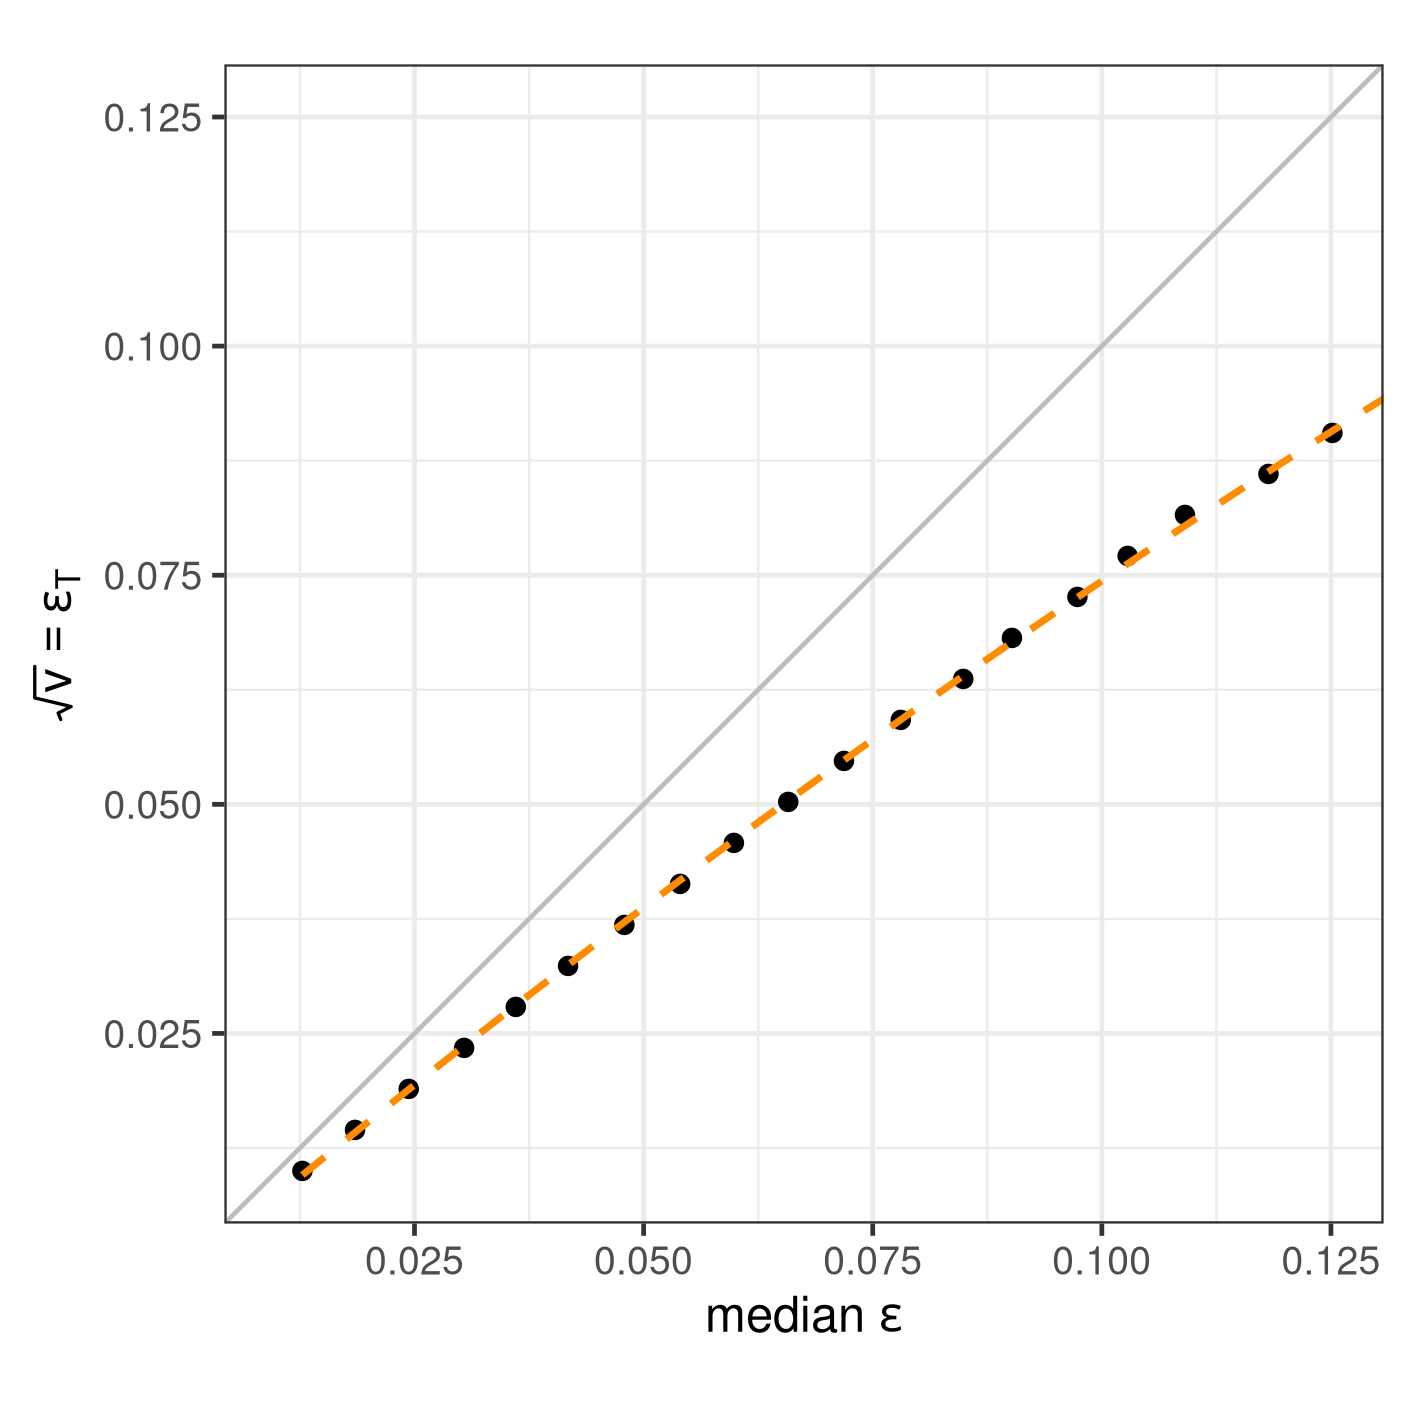
\includegraphics[width=0.8\linewidth]{img/wb-plot} 

}

\caption[The solid gray line indicates where the target RMSEA and median RMSEA values (from 50 samples) would be equal]{The solid gray line indicates where the target RMSEA and median RMSEA values (from 50 samples) would be equal. The dashed orange line indicates the predicted value of $\sqrt{v}$ that will produce a given RMSEA value.}\label{fig:wb-mod-plot}
\end{figure}

In summary, the design of the simulation study was as follows. The crossed combinations of number of factors, number of items per factor, factor correlation, and factor loading configurations correspond to 60 population major factor models. For each of those population models, I generated 500 error-perturbed correlation matrices using three variations of the TKL multiple-target method, the CB method, and the WB method at each of three target model fit conditions corresponding to very good, fair, and poor model fit. In total, this will result in 900 unique conditions and a total of \ensuremath{4.5\times 10^{5}} simulated error-perturbed correlation matrices. All of the independent variables in the study (and the levels of those variables) are summarized in Table \ref{tab:study1-variables}.

\begin{table}[tbp]

\begin{center}
\begin{threeparttable}

\caption{\label{tab:study1-variables}Simulation Study Design Variables and Levels.}

\begin{tabular}{ll}
\toprule
Variable & Levels\\
\midrule
Factors & 1, 3, 5\\
Items/Factor & 5, 15\\
Factor Correlation ($\phi$) & 0.0, 0.3, 0.6\\
Factor Loading & 0.4 , 0.6, 0.8\\
Target Model Fit & Very Good ($\varepsilon_T = 0.025$, $\textrm{CFI}_T = 0.99$),\\
 & Fair ($\varepsilon_T = 0.065$, $\textrm{CFI}_T = 0.95$),\\
 & Poor ($\varepsilon_T = 0.090$, $\textrm{CFI}_T = 0.90$)\\
Model-Error Method & $\textrm{TKL}_{\textrm{RMSEA}}$, $\textrm{TKL}_{\textrm{CFI}}$, $\textrm{TKL}_{\textrm{RMSEA/CFI}}$, CB, WB\\
\bottomrule
\addlinespace
\end{tabular}

\begin{tablenotes}[para]
\normalsize{\textit{Note.} $\varepsilon_T$ = Target RMSEA value; $\textrm{CFI}_T$ = Target CFI value. TKL subscripts indicate which model fit indices were used as targets.}
\end{tablenotes}

\end{threeparttable}
\end{center}

\end{table}

\hypertarget{simulation-procedure}{%
\section{Simulation Procedure}\label{simulation-procedure}}

In the previous section, I described the 60 population models (without model error) resulting from the crossed levels of number of factors, number of items per factor, factor loadings, and factor correlations. In the first stage of the simulation study, I computed the model-implied population correlation matrices for each of the population models using the \texttt{simFA()} function in the R \emph{fungible} library (\protect\hyperlink{ref-waller2021}{Waller, 2021}). The \texttt{simFA()} function computes population correlation matrices for common factor models by taking the model parameters (e.g., factor loadings, number of items per factor, factor correlations) as arguments and then using the equation for the common factor model (i.e., Equation \eqref{eq:cfm}) to produce the population correlation matrix corresponding to the specified model.

After computing model-implied population correlation matrices for each of the 60 population models, the next step in the simulation procedure was to generate population correlation matrices with model error using each of the model-error methods described in the previous section. For each of the \(60 \times 3 = 180\) crossed combinations of population model and target model fit, I generated population correlation matrices with model error

\begin{enumerate}
\def\labelenumi{\arabic{enumi}.}
\tightlist
\item
  TKL
\end{enumerate}

Three variations of the multiple-target TKL method were used to generate population correlation matrices with model error: (\(\textrm{TKL}_\textrm{RMSEA}\), \(\textrm{TKL}_\textrm{CFI}\), and \(\textrm{TKL}_\textrm{RMSEA/CFI}\). For each of these methods, 500 population correlation matrices with model error were generated using random starting values \(\nu_{\textrm{e}0} \sim \mathcal{U}(.2, .9)\) and \(\epsilon_0 \sim \mathcal{U}(0, .8)\), where \(\nu_{\textrm{e}0}\) and \(\epsilon_0\) denote the starting values of \(\nu_{\textrm{e}}\) and \(\epsilon\) and \(\mathcal{U}(a, b)\) denotes a uniform distribution on the interval \([a, b]\). These distributions were chosen because initial testing indicated that the multiple-target TKL method was more likely to result in a converged solution if the range of the starting values were somewhat restricted.

In addition to randomly initializing the starting values of \(\nu_{\textrm{e}}\) and \(\epsilon\), the values of the \(\mathbf{W}^*\) matrix were also randomly initialized at each repetition. In the multiple-target TKL method, the \(p \times q\) provisional matrix \(\mathbf{W}^*\) was initialized such that each column consisted of \(p\) samples from a standard normal distribution. Let \(\epsilon_j\) and \(\nu_{\textrm{e}j}\) denote the proposed values of \(\epsilon\) and \(\nu_{\textrm{e}}\) at iteration \(j\) of the multiple-target TKL optimization procedure. At each \(j\)th iteration, the columns of the \(\mathbf{W}^*\) were scaled using \(\mathbf{W}^*_j = \mathbf{W}^* \mathbf{V}\), where \(\mathbf{V}\) denotes a \(q \times q\) diagonal matrix with diagonal elements \((1-\epsilon_j)^0, (1-\epsilon_j)^1, \dots, (1-\epsilon_j)^q\). Then, \(\mathbf{W}^*_j\) was scaled as described in Section \ref{tkl-method} to form a \(\mathbf{W}_j\) matrix to ensure that the proportion of variance accounted for by the \(q\) minor common factors was equal to \(\nu_{\mathrm{e}j}\).

Repeating each of the TKL method variations 500 times with random starting values was important because the multiple-target TKL method is not guaranteed to find the global optimum for a particular problem. Moreover, the results of the multiple-target TKL method are affected by the particular value of \(\mathbf{W}^*\). Therefore, looking at the results of the multiple-target TKL method with a single set of starting values and a single \(\mathbf{W}^*\) matrix might have led to results that were somewhat idiosyncratic and not representative of the method's general performance.

It might reasonably be asked why \(\mathbf{W}^*\) was not held fixed over the 500 repetitions with random starting values to find the global optimum parameter values \emph{for that particular} \(\mathbf{W}^*\) \emph{matrix}. However, the purpose of the multiple-target TKL method is to produce solutions with fit index values that are ``close enough'' to the target values to be reasonable over the entire space of \(\mathbf{W}^*\) matrices, not to find the best solution for one particular \(\mathbf{W}^*\) matrix.

As with the multiple-target TKL methods, the WB method was also repeated 500 times for each condition of the simulation design. Each repetition of the WB method represented an independent sample from the inverse Wishart distribution associated with each condition. Unlike the multiple-target TKL methods and the WB method, the implementation of the CB method that was used was deterministic. That is, given the same population model, the CB method always returned the same correlation matrix with model error. Therefore, it did not make sense to conduct 500 repetitions of the CB method for each condition because every repetition would have given the exact same result {[}NEED TO MAKE SURE PREVIOUS METHODS SECTION REFLECTS THIS{]}.

Moreover, R code for the simulation study (including implementations of each of the model-error methods) can be found in Appendix A {[}hyperlink this{]}.

\hypertarget{results}{%
\chapter{Results}\label{results}}

In the previous section, I described the simulation study I conducted to learn more about the behavior of different methods for generating error-perturbed population covariance (correlation) matrices. The simulation study included three model-error methods---the (single- and multiple-target) TKL method, the CB method, and the WB method---and was designed to answer two primary questions.

First, I wanted to know whether different model-error methods led to different values of the CFI, TLI, and CRMR fit indices when used with the same error-free models and target RMSEA values. If the model-error methods led to systematically different values on the alternative fit indices when matched on RMSEA and all other characteristics, it would suggest that they are not exchangeable. In that case, researchers conducting simulation studies would have to consider which of the model-error methods most closely approximates the model error process they are trying to simulate. Moreover, such results would highlight the importance of reporting fit indices other than RMSEA when simulating imperfect models. If there were no meaningful differences among the methods, it would indicate that the choice of one particular model-error method over another (among the methods considered here) is not an important variable in the design of simulation studies.

A second purpose of the study was to evaluate the effectiveness of the proposed multiple-target method for generating correlation matrices with model error that had RMSEA and CFI values that were close to the specified target values. It was not expected that the algorithm would be able to produce correlation matrices with RMSEA and CFI values that were very close to the target values for all of the major-factor population models because of the relationship between RMSEA, CFI, and population model characteristics (\protect\hyperlink{ref-lai2016}{Lai \& Green, 2016}). Therefore, I used the absolute deviation between the observed and target RMSEA and CFI values to compare the results from the multiple-target TKL method to the results from the CB and WB methods used in Study 1.

The remainder of the section is structured as follows. First, I report how many of the simulated matrices had properties that would make them unsuitable for use in a simulation study. XXX\ldots{}

\hypertarget{indefinite-matrices-cb}{%
\section{Indefinite Matrices (CB)}\label{indefinite-matrices-cb}}

One drawback of the CB model-error method is that the resulting correlation matrix with model error can be indefinite (i.e.~having one or more negative eigenvalues) when the specified target RMSEA value is large (\protect\hyperlink{ref-cudeck1992}{Cudeck \& Browne, 1992}). These matrices are undesirable because correlation and covariance matrices are, by definition, at least positive semi definite (i.e., having strictly non-negative eigenvalues). Of the 90000 correlation matrices with model error that were generated using the CB method, 14291 (15.9\%) were indefinite. However, indefinite solutions were much more common for some conditions of the simulation design than other. Figure \ref{fig:fig-percent-indefinite-matrices} shows the percent of indefinite CB solutions for each level of model fit, number of items per factor, number of factors, and factor loading strength are shown in Figure \ref{fig:fig-percent-indefinite-matrices}. (Exact percentages are reported in Table \ref{tab:tab-percent-indefinite-matrices}). The figure shows at least three notable trends. First, the percent of indefinite solutions increased as model fit degraded. Second, the percent of indefinite solutions increased as the total number of items increased (i.e., as the number of factors and items per factor increased). Finally, Figure \ref{fig:fig-percent-indefinite-matrices} shows that the percent of indefinite solutions increased as factor loadings increased.

In the best-case scenarios, conditions corresponding to models with 25 items or fewer led to indefinite solutions very infrequently (in less than 1\% of cases). On the other hand, conditions with Poor model fit and 45 items or more led to indefinite correlation matrices in more than 90\% of cases. These results show that the CB method would be an inefficient way to simulate positive semi definite population correlation or covariance matrices with model error when input matrices are large and the target RMSEA value is relatively large.

Although inefficient, a potential strategy for dealing with indefinite solutions when using the CB method is to simply generate solutions using the CB method until a sufficient number of positive semi definite solutions have been obtained. However, the amount of time taken by the CB method increases quickly as the number of items increase, making the oversampling strategy impractical for problems with many items. In fact, using the CB method to generate even a small number of solution matrices becomes impractical for large input matrices. This is demonstrated in Figure \ref{fig:cb-completion-time}, which shows the completion time for the CB method when applied to a one-factor model with salient loadings fixed at .6 and the number of items varying between 5 and 120. Using a computer with an Intel Core i5-4570 3.20GHz CPU and 16GB of RAM, the CB method took just over 30 seconds to complete (on average) for an input correlation matrix with 65 items. For an input matrix with 115 items, the CB method took approximately four and a half minutes to complete. Long completion times are often impractical for large simulation studies, particularly if indefinite solutions are discarded. In fact, I had to skip using the CB method in simulation conditions with 10 factors and 15 items per factor (150 items) because those conditions would have taken an impractical amount of time to complete. Timing a single example, the CB method took 15 minutes and 48 seconds to complete with a 150-item input correlation matrix. At that rate, it would have taken almost 11 days to complete one (out of 36) conditions of the simulation design with 150 items.



\begin{verbatim}
`summarise()` has grouped output by 'factors', 'items_per_factor',
'loading_numeric'. You can override using the `.groups` argument.
\end{verbatim}

\begin{table}[tbp]

\begin{center}
\begin{threeparttable}

\caption{\label{tab:tab-percent-indefinite-matrices}The percent of Cudeck and Browne (CB) model-error method solutions that were indefinite.}

\begin{tabular}{rrlrrrr}
\toprule
 &  &  & \multicolumn{4}{c}{Factors} \\
\cmidrule(r){4-7}
Items/Factor & Loading & Model Fit & 1 & 3 & 5 & 10\\
\midrule
5 & 0.4 & Very Good & 0.0 & 0.0 & 0.0 & 0.0\\
5 & 0.4 & Fair & 0.0 & 0.3 & 0.1 & 0.0\\
5 & 0.4 & Poor & 0.0 & 0.1 & 1.1 & 0.3\\
5 & 0.6 & Very Good & 0.0 & 0.0 & 0.0 & 0.0\\
5 & 0.6 & Fair & 0.0 & 0.0 & 0.7 & 0.0\\
5 & 0.6 & Poor & 0.2 & 0.4 & 0.9 & 0.5\\
5 & 0.8 & Very Good & 0.0 & 0.0 & 0.0 & 0.0\\
5 & 0.8 & Fair & 0.0 & 0.1 & 0.1 & 0.0\\
5 & 0.8 & Poor & 0.0 & 0.7 & 1.3 & 0.7\\
15 & 0.4 & Very Good & 0.0 & 0.0 & 0.3 & ---\\
15 & 0.4 & Fair & 0.2 & 1.7 & 68.7 & ---\\
15 & 0.4 & Poor & 0.4 & 91.7 & 99.1 & ---\\
15 & 0.6 & Very Good & 0.0 & 0.0 & 0.0 & ---\\
15 & 0.6 & Fair & 0.2 & 2.2 & 75.1 & ---\\
15 & 0.6 & Poor & 1.4 & 91.2 & 98.9 & ---\\
15 & 0.8 & Very Good & 0.0 & 0.0 & 0.1 & ---\\
15 & 0.8 & Fair & 0.2 & 1.7 & 76.5 & ---\\
15 & 0.8 & Poor & 0.4 & 93.4 & 99.0 & ---\\
\bottomrule
\addlinespace
\end{tabular}

\begin{tablenotes}[para]
\normalsize{\textit{Note.} The Cudeck-Browne method was not used for conditions with 10 major factors and 15 items per factor because it was prohibitively slow for those conditions.}
\end{tablenotes}

\end{threeparttable}
\end{center}

\end{table}

\begin{figure}

{\centering 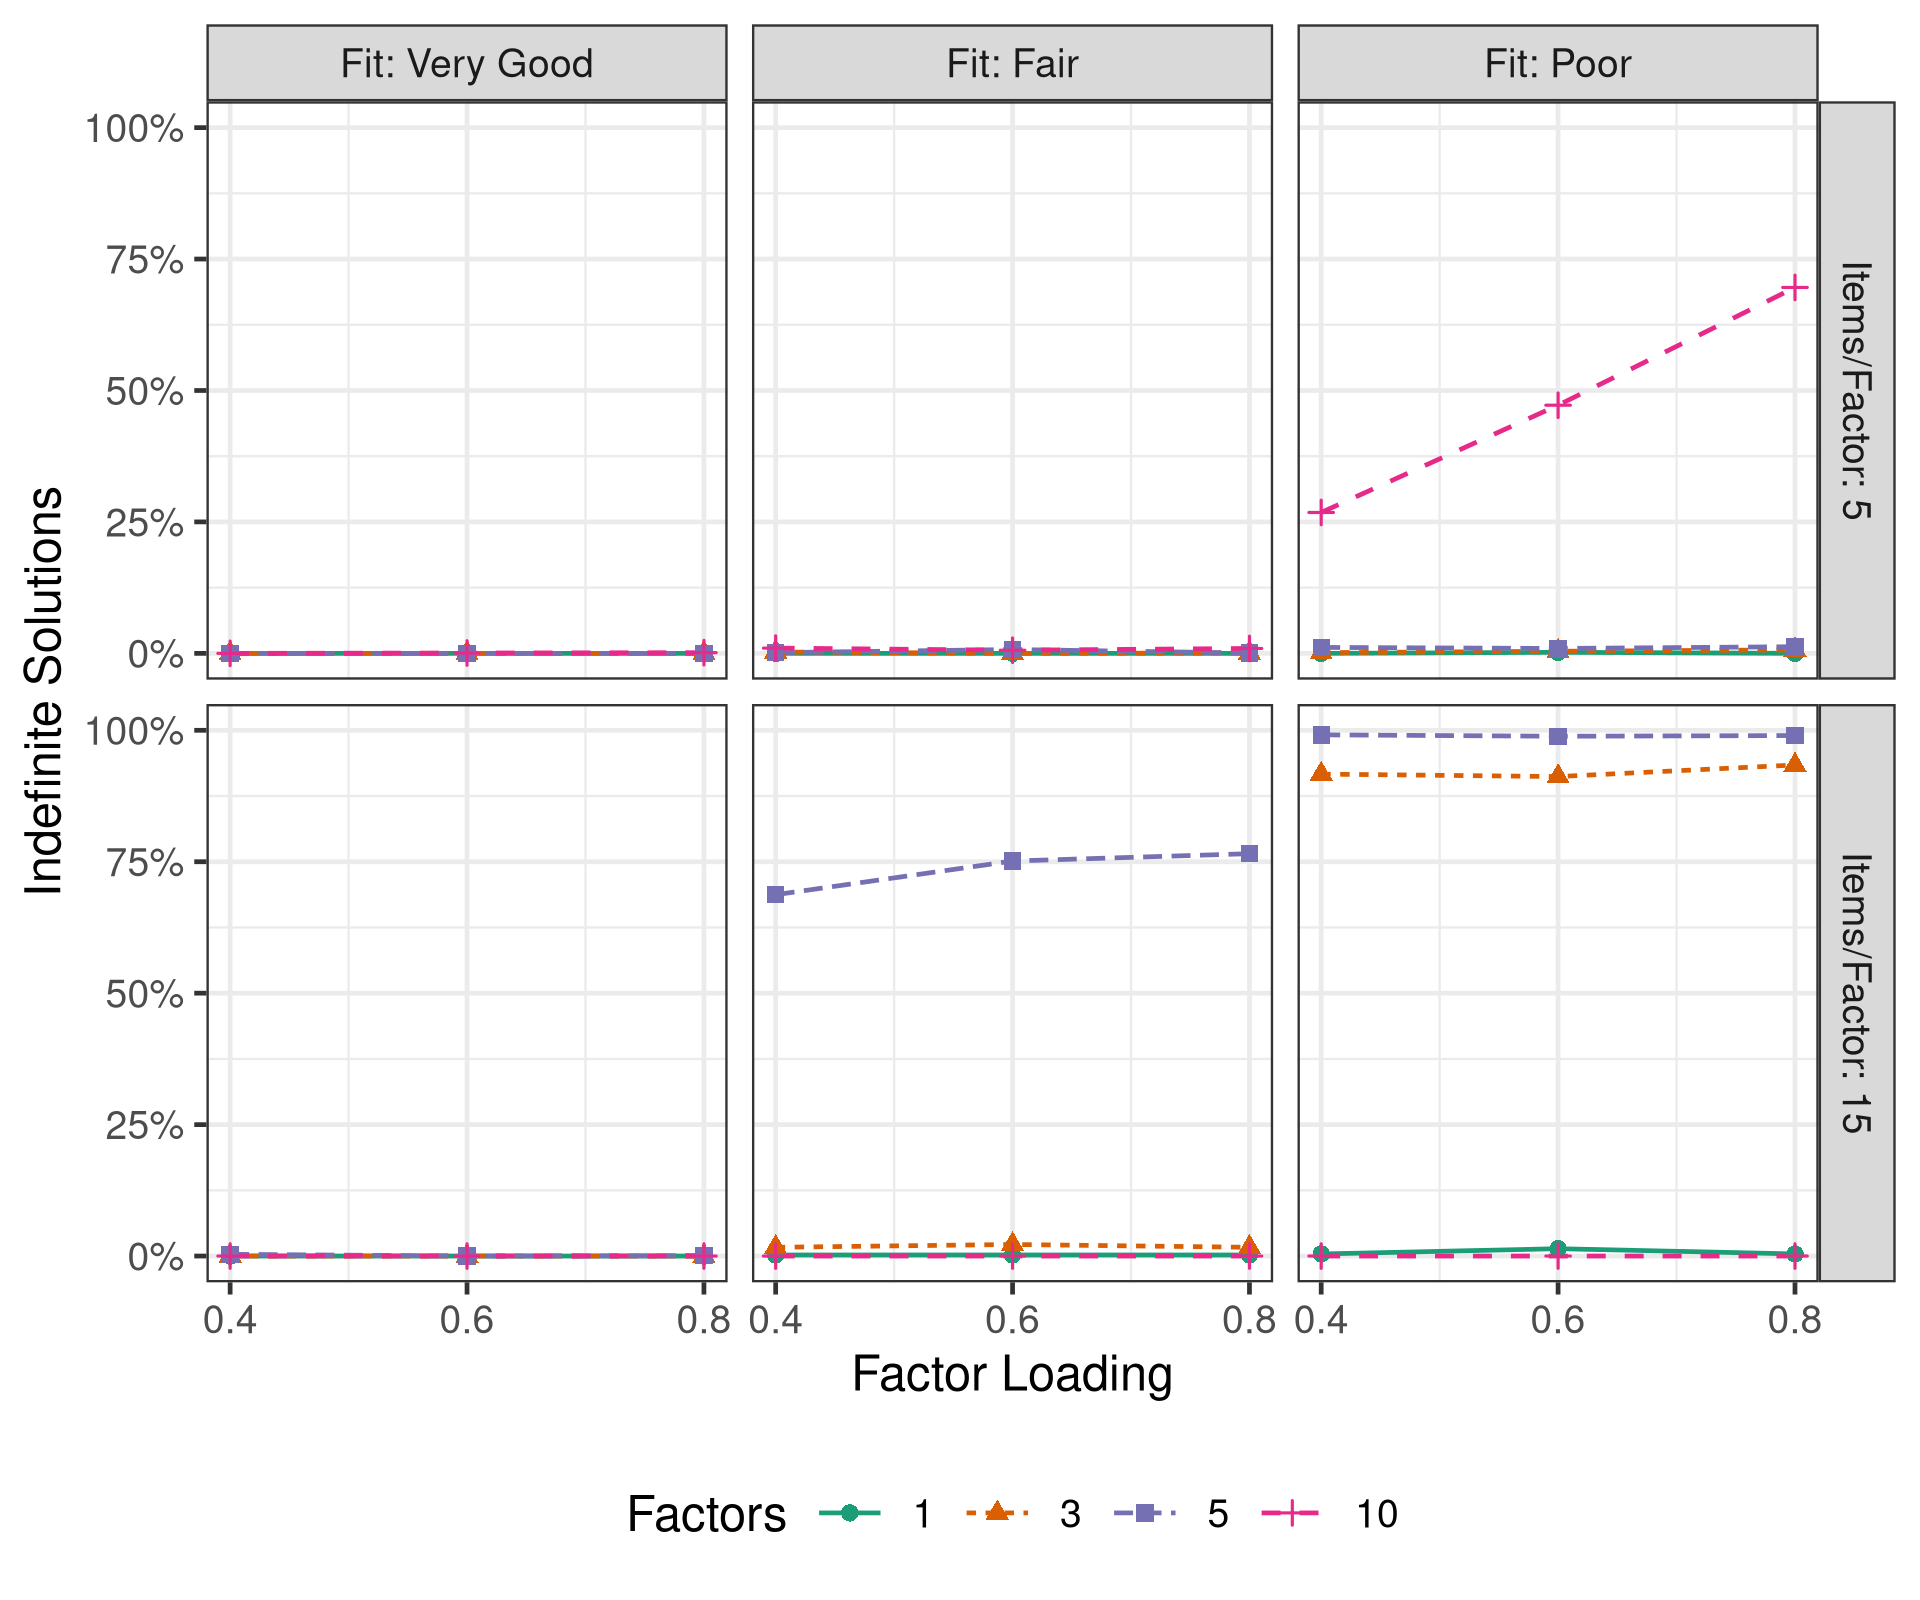
\includegraphics[width=0.8\linewidth]{img/cb_percent_indefinite} 

}

\caption[The percent of Cudeck-Browne (CB) method solutions that were indefinite, conditioned on number of factors, factor loading, number of items per factor, and model fit]{The percent of Cudeck-Browne (CB) method solutions that were indefinite, conditioned on number of factors, factor loading, number of items per factor, and model fit.}\label{fig:fig-percent-indefinite-matrices}
\end{figure}

\begin{figure}

{\centering 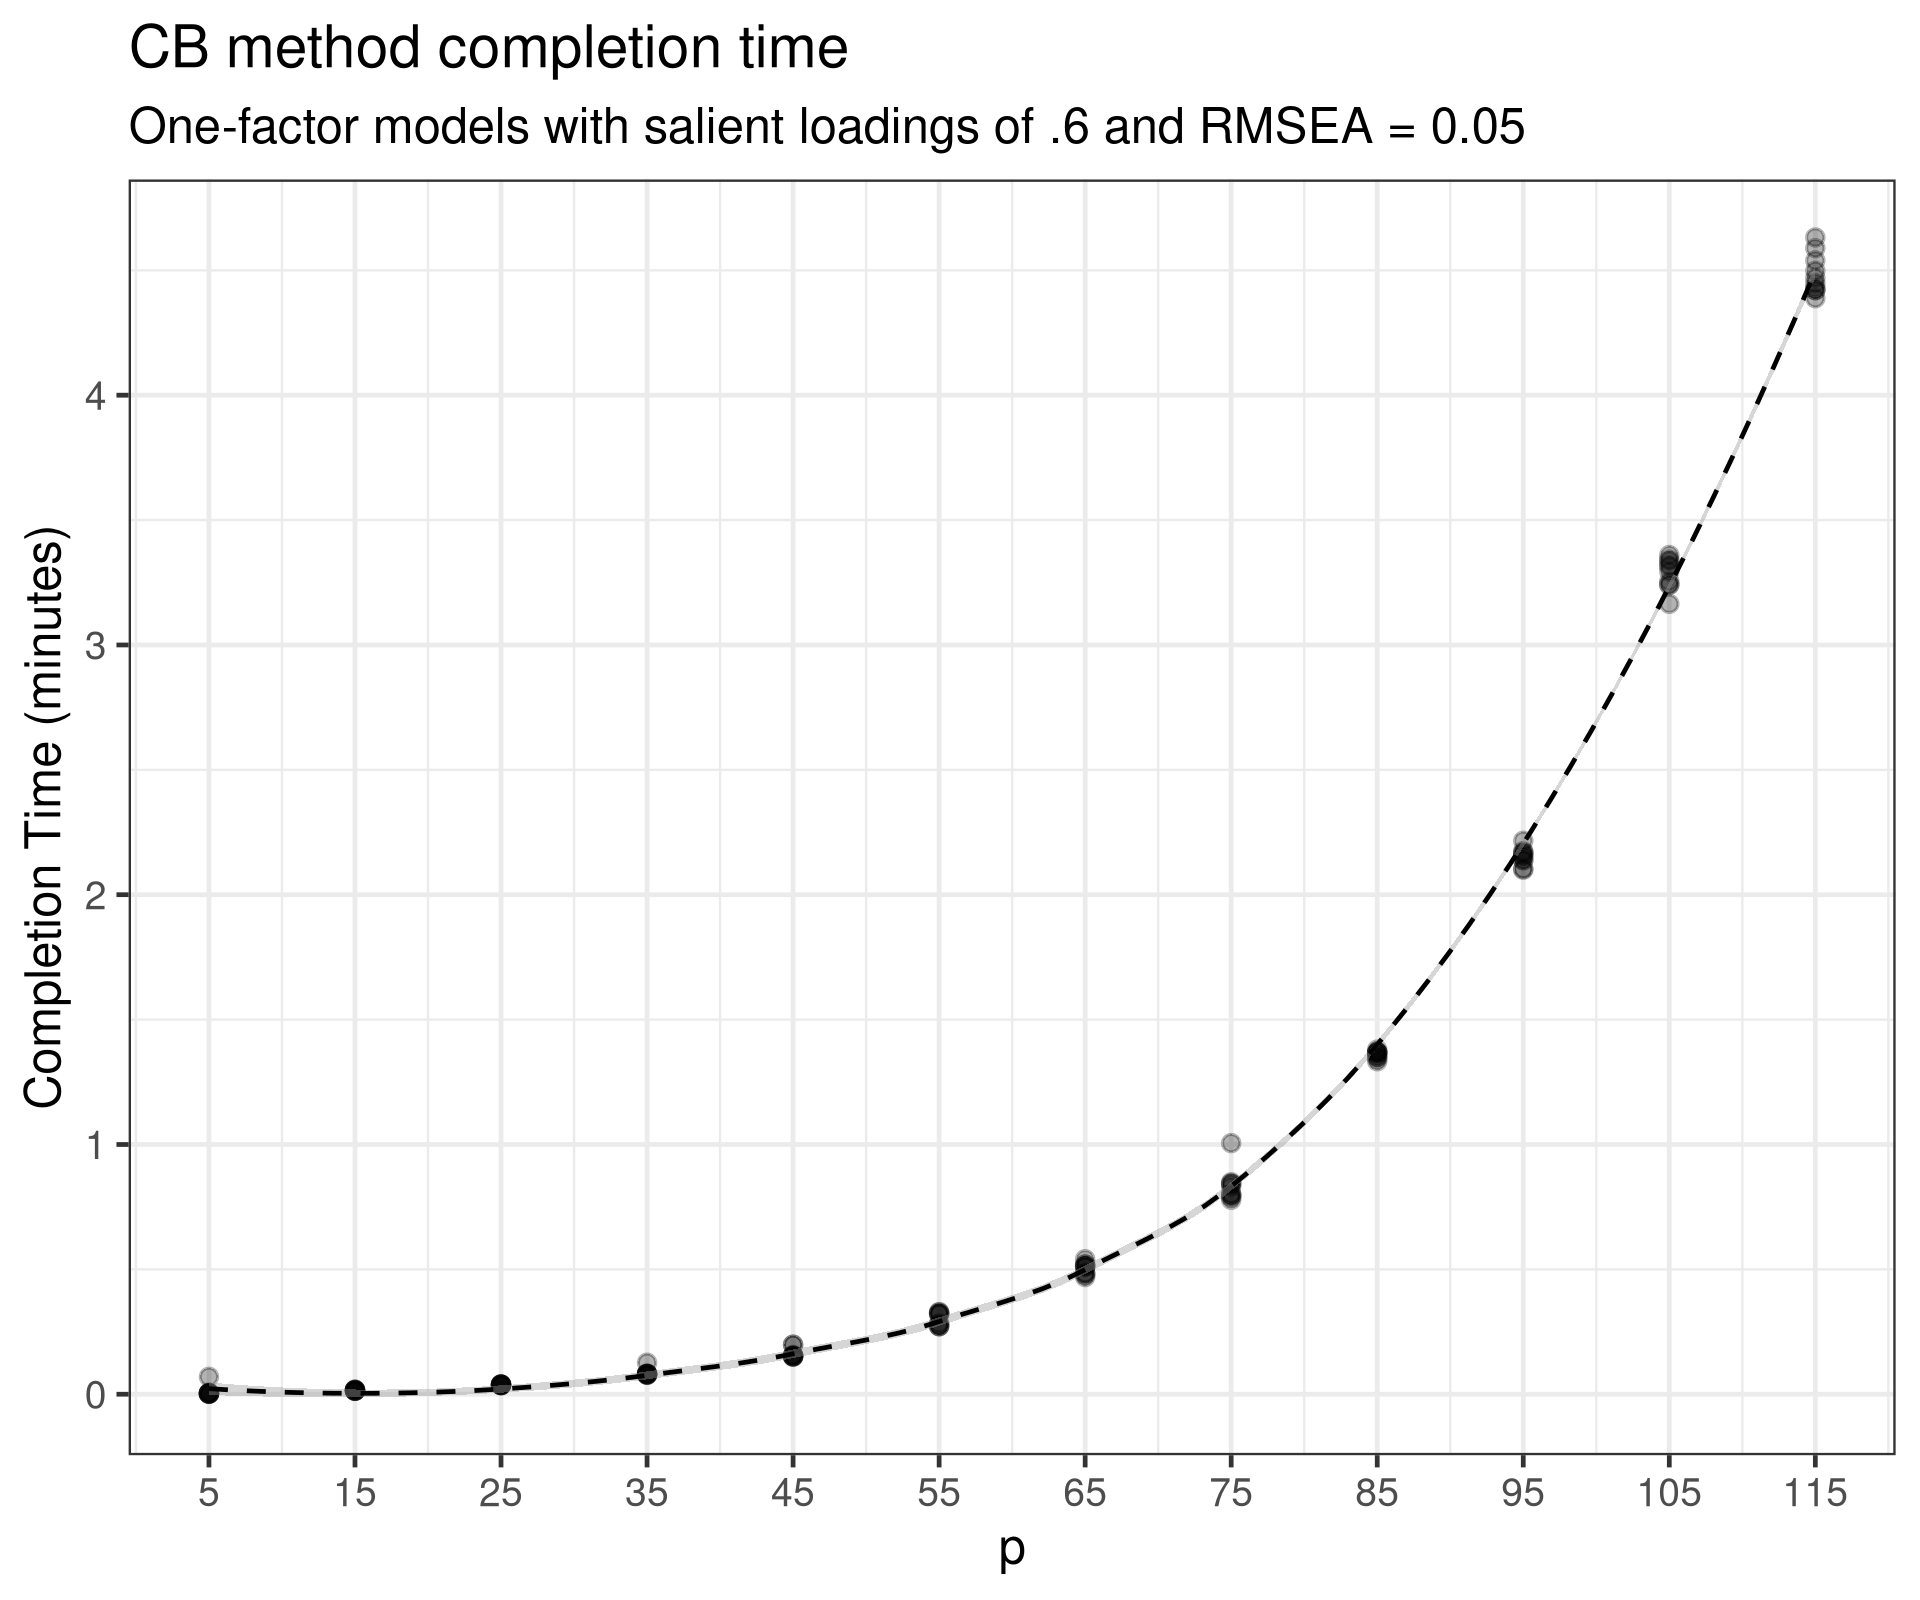
\includegraphics[width=0.8\linewidth]{/home/justin/Documents/dissertation/img/cb_time_plot} 

}

\caption[The amount of time (in minutes) taken to generate a single correlation matrix with model error using the CB method]{The amount of time (in minutes) taken to generate a single correlation matrix with model error using the CB method. Completion times were recorded 10 times for single-factor models with salient factor loadings fixed at .6 and number of items (*p*) varying between 5 and 115. The dashed black line is the loess regression line.}\label{fig:cb-completion-time}
\end{figure}

\hypertarget{l-bfgs-b-non-convergence-genetic-algorithm}{%
\section{L-BFGS-B Non-convergence (Genetic Algorithm)}\label{l-bfgs-b-non-convergence-genetic-algorithm}}

The default optimization method for the multiple-target TKL method was L-BFGS-B. In most cases, this method worked well and converged relatively quickly to a solution. However, there were a small number of cases where the L-BGFS-B method failed to converge. Specifically, the L-BFGS-B method failed to converge 14 times (\(<1\)\%) when the target CFI and RMSEA values were both used and when model fit was poor. The L-BFGS-B non-convergence rates for the \(\textrm{TKL}_{\textrm{RMSEA/CFI}}\) method by number of factors, number of items per factor, and model fit are shown in Table \ref{tab:tab-l-bfgs-b-convergence}. Non-convergence was also somewhat more likely for conditions with few factors compared to conditions with many factors.

Although non-convergence of the L-BFGS-B algorithm was rare, a question that arose was whether the genetic algorithm that was used as a fallback option led to similar results compared to cases where the L-BFGS-B algorithm converged. This question was difficult to answer statistically because non-convergence occurred so infrequently. To get a general sense of whether results for cases where the L-BFGS-B algorithm converged or did not converge were similar, I plotted the CFI and RMSEA values for all converged and non-converged cases in conditions where the multiple-target TKL method was used with target CFI and RMSEA values and model fit was Poor. Figure \ref{fig:comparison-of-converged-vs-non-converged} shows that cases where the L-BFGS-B algorithm did not converge (shown in black) led to similar RMSEA and CFI values compared to cases where the algorithm converged (shown in gray). Thus, using a genetic algorithm seemed to provide reasonable results in the few cases where the L-BFGS-B algorithm failed to converge (albeit much more slowly than the L-BFGS-B algorithm).

\begin{figure}

{\centering 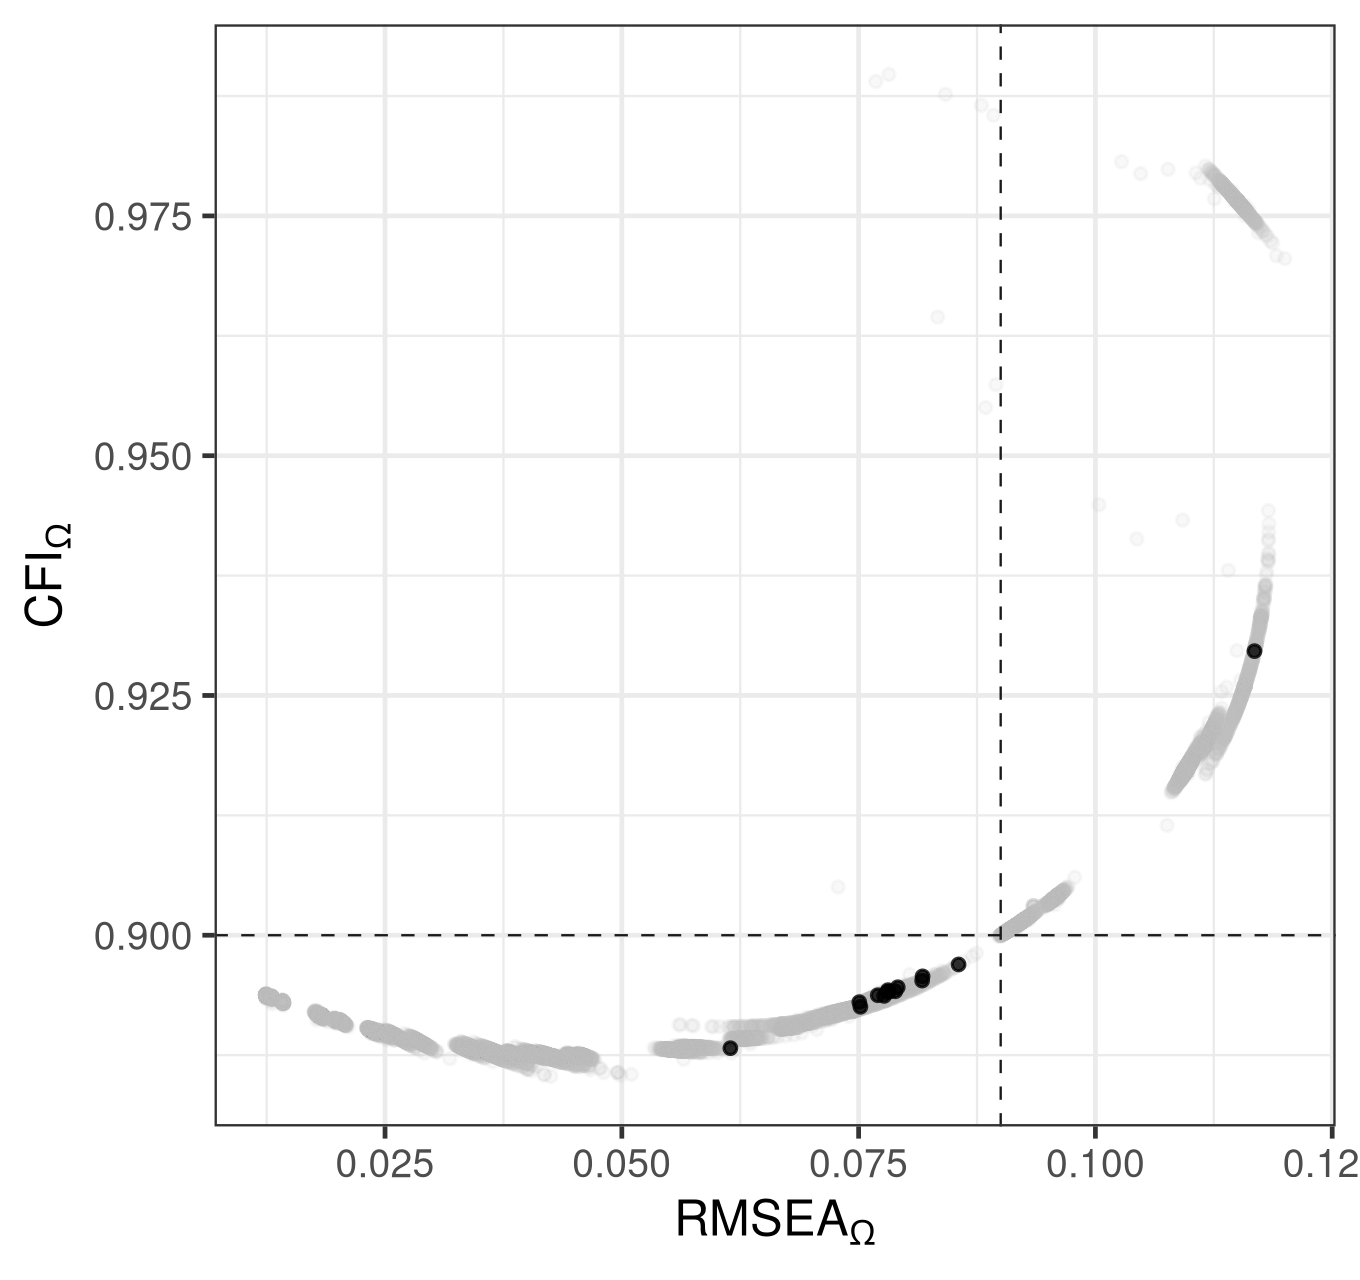
\includegraphics[width=0.8\linewidth]{/home/justin/Documents/dissertation/img/nonconverged_rmsea_cfi} 

}

\caption[RMSEA and CFI values for cases where the model-error method was $\textrm{TKL}_{\textrm{RMSEA/CFI}}$ and model fit was Poor]{RMSEA and CFI values for cases where the model-error method was $\textrm{TKL}_{\textrm{RMSEA/CFI}}$ and model fit was Poor. Grey dots indicate cases where the L-BFGS-G algorithm converged; black dots indicate cases that did not converge and where a genetic algorithm was used instead.}\label{fig:comparison-of-converged-vs-non-converged}
\end{figure}



\begin{verbatim}
`summarise()` has grouped output by 'factors', 'model_fit'. You can override
using the `.groups` argument.
\end{verbatim}

\begin{table}[tbp]

\begin{center}
\begin{threeparttable}

\caption{\label{tab:tab-l-bfgs-b-convergence}The percent of cases in each combination of conditions where the L-BFGS-B algorithm did not converge after 100 random starts and genetic optimization was used instead.}

\small{

\begin{tabular}{rlrrr}
\toprule
 &  & \multicolumn{3}{c}{Model Fit} \\
\cmidrule(r){3-5}
Factors & Items/Factor & Very Good & Fair & Poor\\
\midrule
1 & 5 & 0.0 & 0.0 & 0.1\\
1 & 15 & 0.0 & 0.0 & 0.4\\
3 & 5 & 0.0 & 0.0 & 0.1\\
3 & 15 & 0.0 & 0.0 & 0.0\\
5 & 5 & 0.0 & 0.0 & 0.0\\
5 & 15 & 0.0 & 0.0 & 0.0\\
10 & 5 & 0.0 & 0.0 & 0.0\\
10 & 15 & 0.0 & 0.0 & 0.0\\
\bottomrule
\end{tabular}

}

\end{threeparttable}
\end{center}

\end{table}

\hypertarget{major-minor-factors-w-matrices}{%
\section{Major Minor Factors (W Matrices)}\label{major-minor-factors-w-matrices}}

Recall that the multiple-objective TKL method included an optional penalty that heavily penalized cases that had strong minor factors. Specifically, the penalty was applied if any minor factor had two or more absolute factor loadings greater than or equal to a specified value. The purpose of the penalty was to avoid introducing minor factors that might be more accurately characterized as major factors. To determine whether the penalty was effective at helping avoid major minor factors, I checked each of the minor factor loading (\(\mathbf{W}\)) matrices to determine whether any minor factor had two or more loadings greater than .3 (in absolute value).

The percent of cases where the constraints on \(\mathbf{W}\) were violated for each level of number of factors, number of items per factor, factor loading strength, and model fit are shown in Figure \ref{fig:w-major-factors-plot} and reported in Table \ref{tab:tab-major-minor-factors}. Only results for the \(\textrm{TKL}_{\textrm{RMSEA}}\) were included because the \(\textrm{TKL}_{\textrm{RMSEA/CFI}}\) and \(\textrm{TKL}_{\textrm{CFI}}\) error methods seldom led to solutions that violated the constraints on \(\mathbf{W}\). (Only 24 out of 90,000 cases had violated \(\mathbf{W}\) constraints for the \(\textrm{TKL}_{\textrm{RMSEA/CFI}}\) and \(\textrm{TKL}_{\textrm{CFI}}\) methods combined). Figure \ref{fig:w-major-factors-plot} shows that the \(\mathbf{W}\) constraints were violated most often when model fit was Fair or Poor, factor loadings were relatively low, and there were many total items (i.e., many factors and items per factor).

To understand why certain conditions led to more \(\mathbf{W}\) constraint violations than others, it is helpful to understand the relationship between those conditions and the TKL parameters (\(\epsilon\) and \(\nu_{\textrm{e}}\)). Figure \ref{fig:eps-and-v-values-by-W-violations} shows the \(\epsilon\) and \(\nu_{\textrm{e}}\) values for each of the TKL model-error methods, conditioned on factor loading strength, number of factors, and number of items per factor. To conserve space, only conditions with Poor model fit and 1, 5, or 10 major factors were included in the figure. Overall, the figure shows that there was a trade-off between \(\epsilon\) and \(\nu_{\textrm{e}}\) such that higher values of \(\nu_{\textrm{e}}\) were related to lower values of \(\epsilon\) (and \emph{vice versa}). Moreover, Figure \ref{fig:eps-and-v-values-by-W-violations} shows that the distributions of \(\epsilon\) and \(\nu_{\textrm{e}}\) differed depending on which TKL variant was used. The differences between the error-method variants were largest when the there were many items (i.e., many items and many items per factor) and when factor loadings were relatively weak. Under those circumstances, the \(\textrm{TKL}_\textrm{RMSEA}\) method led to higher values of \(\nu_{\textrm{e}}\) than the \(\textrm{TKL}_\textrm{RMSEA/CFI}\) or \(\textrm{TKL}_\textrm{CFI}\) methods. This effect suggests that higher values of \(\nu_{\textrm{e}}\) were required to produce solutions with RMSEA values close to .09 when there are many items. On the other hand, the results for the \(\textrm{TKL}_\textrm{RMSEA/CFI}\) and \(\textrm{TKL}_\textrm{CFI}\) methods indicated that much lower \(\nu_{\textrm{e}}\) values were required to obtain CFI values close to .90 when there were many items.

The apparent trade-off between \(\epsilon\) and \(\nu_{\textrm{e}}\) values makes sense when you consider their roles in the TKL method. A high \(\nu_{\textrm{e}}\) value indicated that much of the unique variance would be assigned to the minor common factors. If the value of \(\epsilon\) was also high, it indicated that the first few minor factors would account for most of the minor factor variance. Therefore, the \(\mathbf{W}\) constraints were more likely to be violated when both \(\epsilon\) and \(\nu_{\textrm{e}}\) were high and less likely to be violated if either parameter was low. in Figure \ref{fig:eps-and-v-values-by-W-violations}, which shows the values of \(\epsilon\) and \(\nu_{\textrm{e}}\) produced by the three TKL variants for conditions with Poor model fit, 10 factors, 15 items per factor, and factor loadings of .8. Each point (corresponding to a single case) was colored according to whether or not the \(\mathbf{W}\) constraints were violated. The figure shows that the \(\mathbf{W}\) constraints were violated when the values of \(\epsilon\) and \(\nu_{\textrm{e}}\) were both above some threshold, which only happened when the \(\textrm{TKL}_\textrm{RMSEA}\) was used.



\begin{verbatim}
`summarise()` has grouped output by 'factors', 'items_per_factor',
'loading_numeric'. You can override using the `.groups` argument.
\end{verbatim}

\begin{table}[tbp]

\begin{center}
\begin{threeparttable}

\caption{\label{tab:tab-major-minor-factors}The percent of cases that violated the minor common factor loading constraints for each level of number of factors, items per factor, factor loading, and model fit when the \(\textrm{TKL}_{\textrm{RMSEA}}\) method was used.}

\small{

\begin{tabular}{rrlrrr}
\toprule
 &  &  & \multicolumn{3}{c}{Model Fit} \\
\cmidrule(r){4-6}
Factors & Items per Factor & Loading & Very Good & Fair & Poor\\
\midrule
1 & 5 & 0.4 & 0.0 & 0.0 & 0.0\\
1 & 5 & 0.6 & 0.0 & 0.0 & 0.0\\
1 & 5 & 0.8 & 0.0 & 0.0 & 0.0\\
1 & 15 & 0.4 & 0.0 & 3.2 & 39.4\\
1 & 15 & 0.6 & 0.0 & 0.0 & 15.0\\
1 & 15 & 0.8 & 0.0 & 0.0 & 0.0\\
3 & 5 & 0.4 & 0.0 & 0.1 & 22.9\\
3 & 5 & 0.6 & 0.0 & 0.0 & 4.7\\
3 & 5 & 0.8 & 0.0 & 0.0 & 0.0\\
3 & 15 & 0.4 & 0.0 & 57.3 & 79.3\\
3 & 15 & 0.6 & 0.0 & 33.3 & 74.9\\
3 & 15 & 0.8 & 0.0 & 0.0 & 7.4\\
5 & 5 & 0.4 & 0.0 & 4.8 & 52.3\\
5 & 5 & 0.6 & 0.0 & 0.0 & 34.5\\
5 & 5 & 0.8 & 0.0 & 0.0 & 0.0\\
5 & 15 & 0.4 & 0.0 & 79.0 & 92.6\\
5 & 15 & 0.6 & 0.0 & 73.3 & 89.7\\
5 & 15 & 0.8 & 0.0 & 0.0 & 81.2\\
10 & 5 & 0.4 & 0.0 & 44.7 & 75.9\\
10 & 5 & 0.6 & 0.0 & 12.1 & 68.9\\
10 & 5 & 0.8 & 0.0 & 0.0 & 1.6\\
10 & 15 & 0.4 & 0.0 & 94.5 & 99.9\\
10 & 15 & 0.6 & 0.0 & 94.8 & 98.3\\
10 & 15 & 0.8 & 0.0 & 82.3 & 96.8\\
\bottomrule
\end{tabular}

}

\end{threeparttable}
\end{center}

\end{table}

\begin{figure}

{\centering 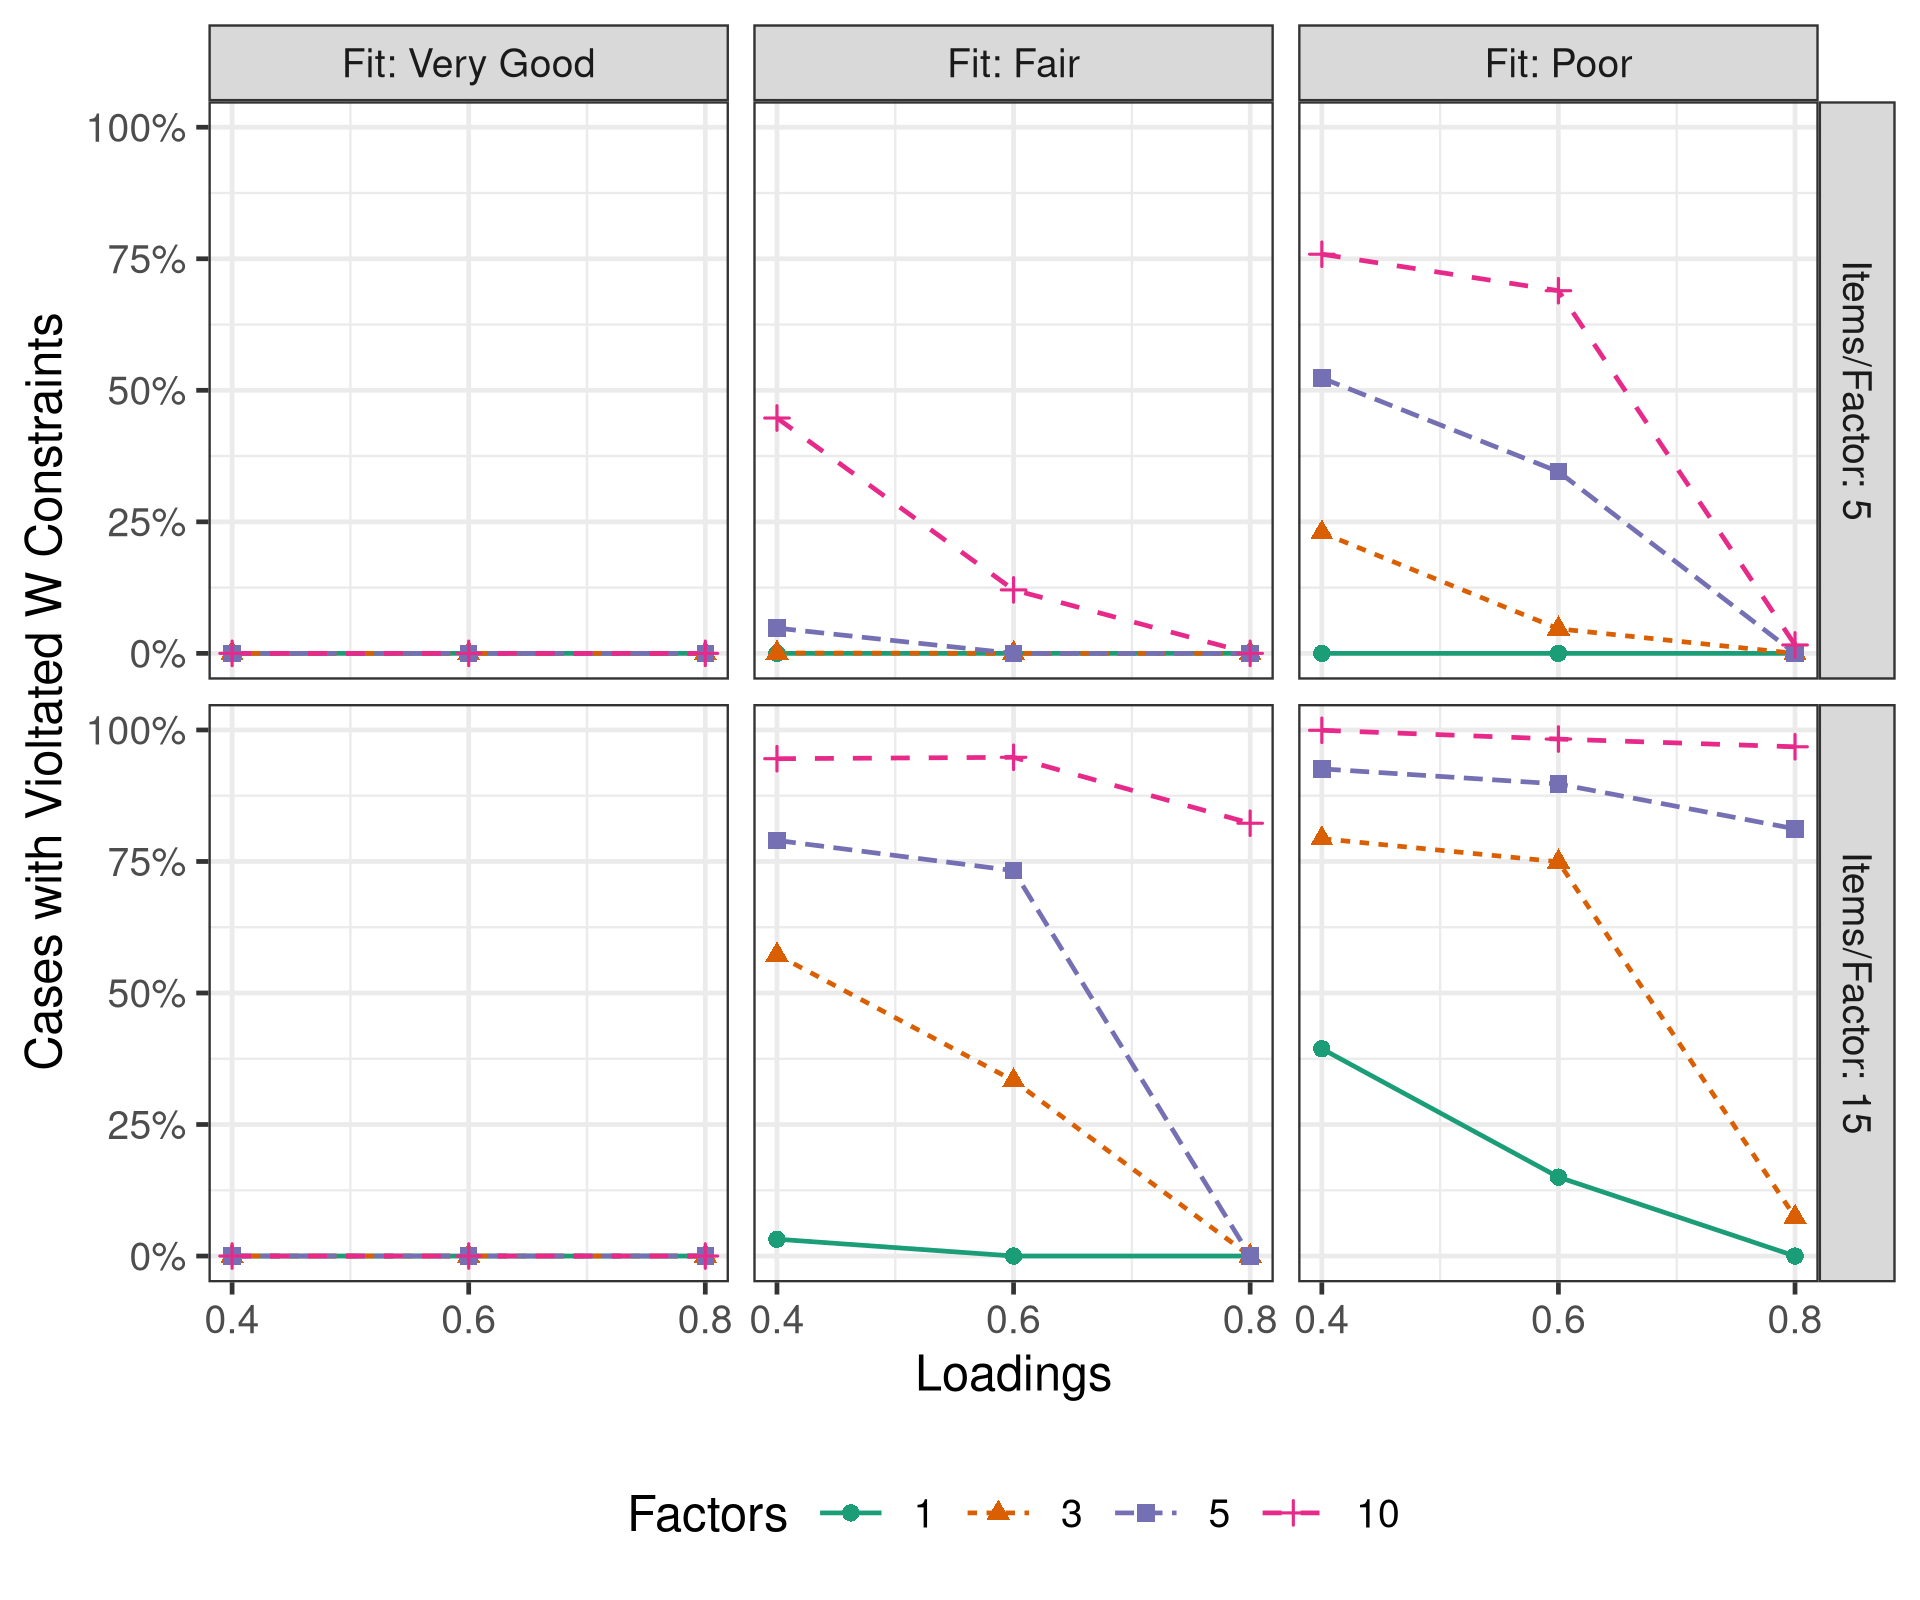
\includegraphics[width=0.8\linewidth]{/home/justin/Documents/dissertation/img/major_minor_factors} 

}

\caption[The percent of cases where the constraints on $\mathbf{W}$ were violated when the $\textrm{TKL}_{\textrm{RMSEA}}$ model-error method was used for each level of number of factors, number of items per factor, factor loading, and model fit]{The percent of cases where the constraints on $\mathbf{W}$ were violated when the $\textrm{TKL}_{\textrm{RMSEA}}$ model-error method was used for each level of number of factors, number of items per factor, factor loading, and model fit.}\label{fig:w-major-factors-plot}
\end{figure}

\begin{figure}

{\centering 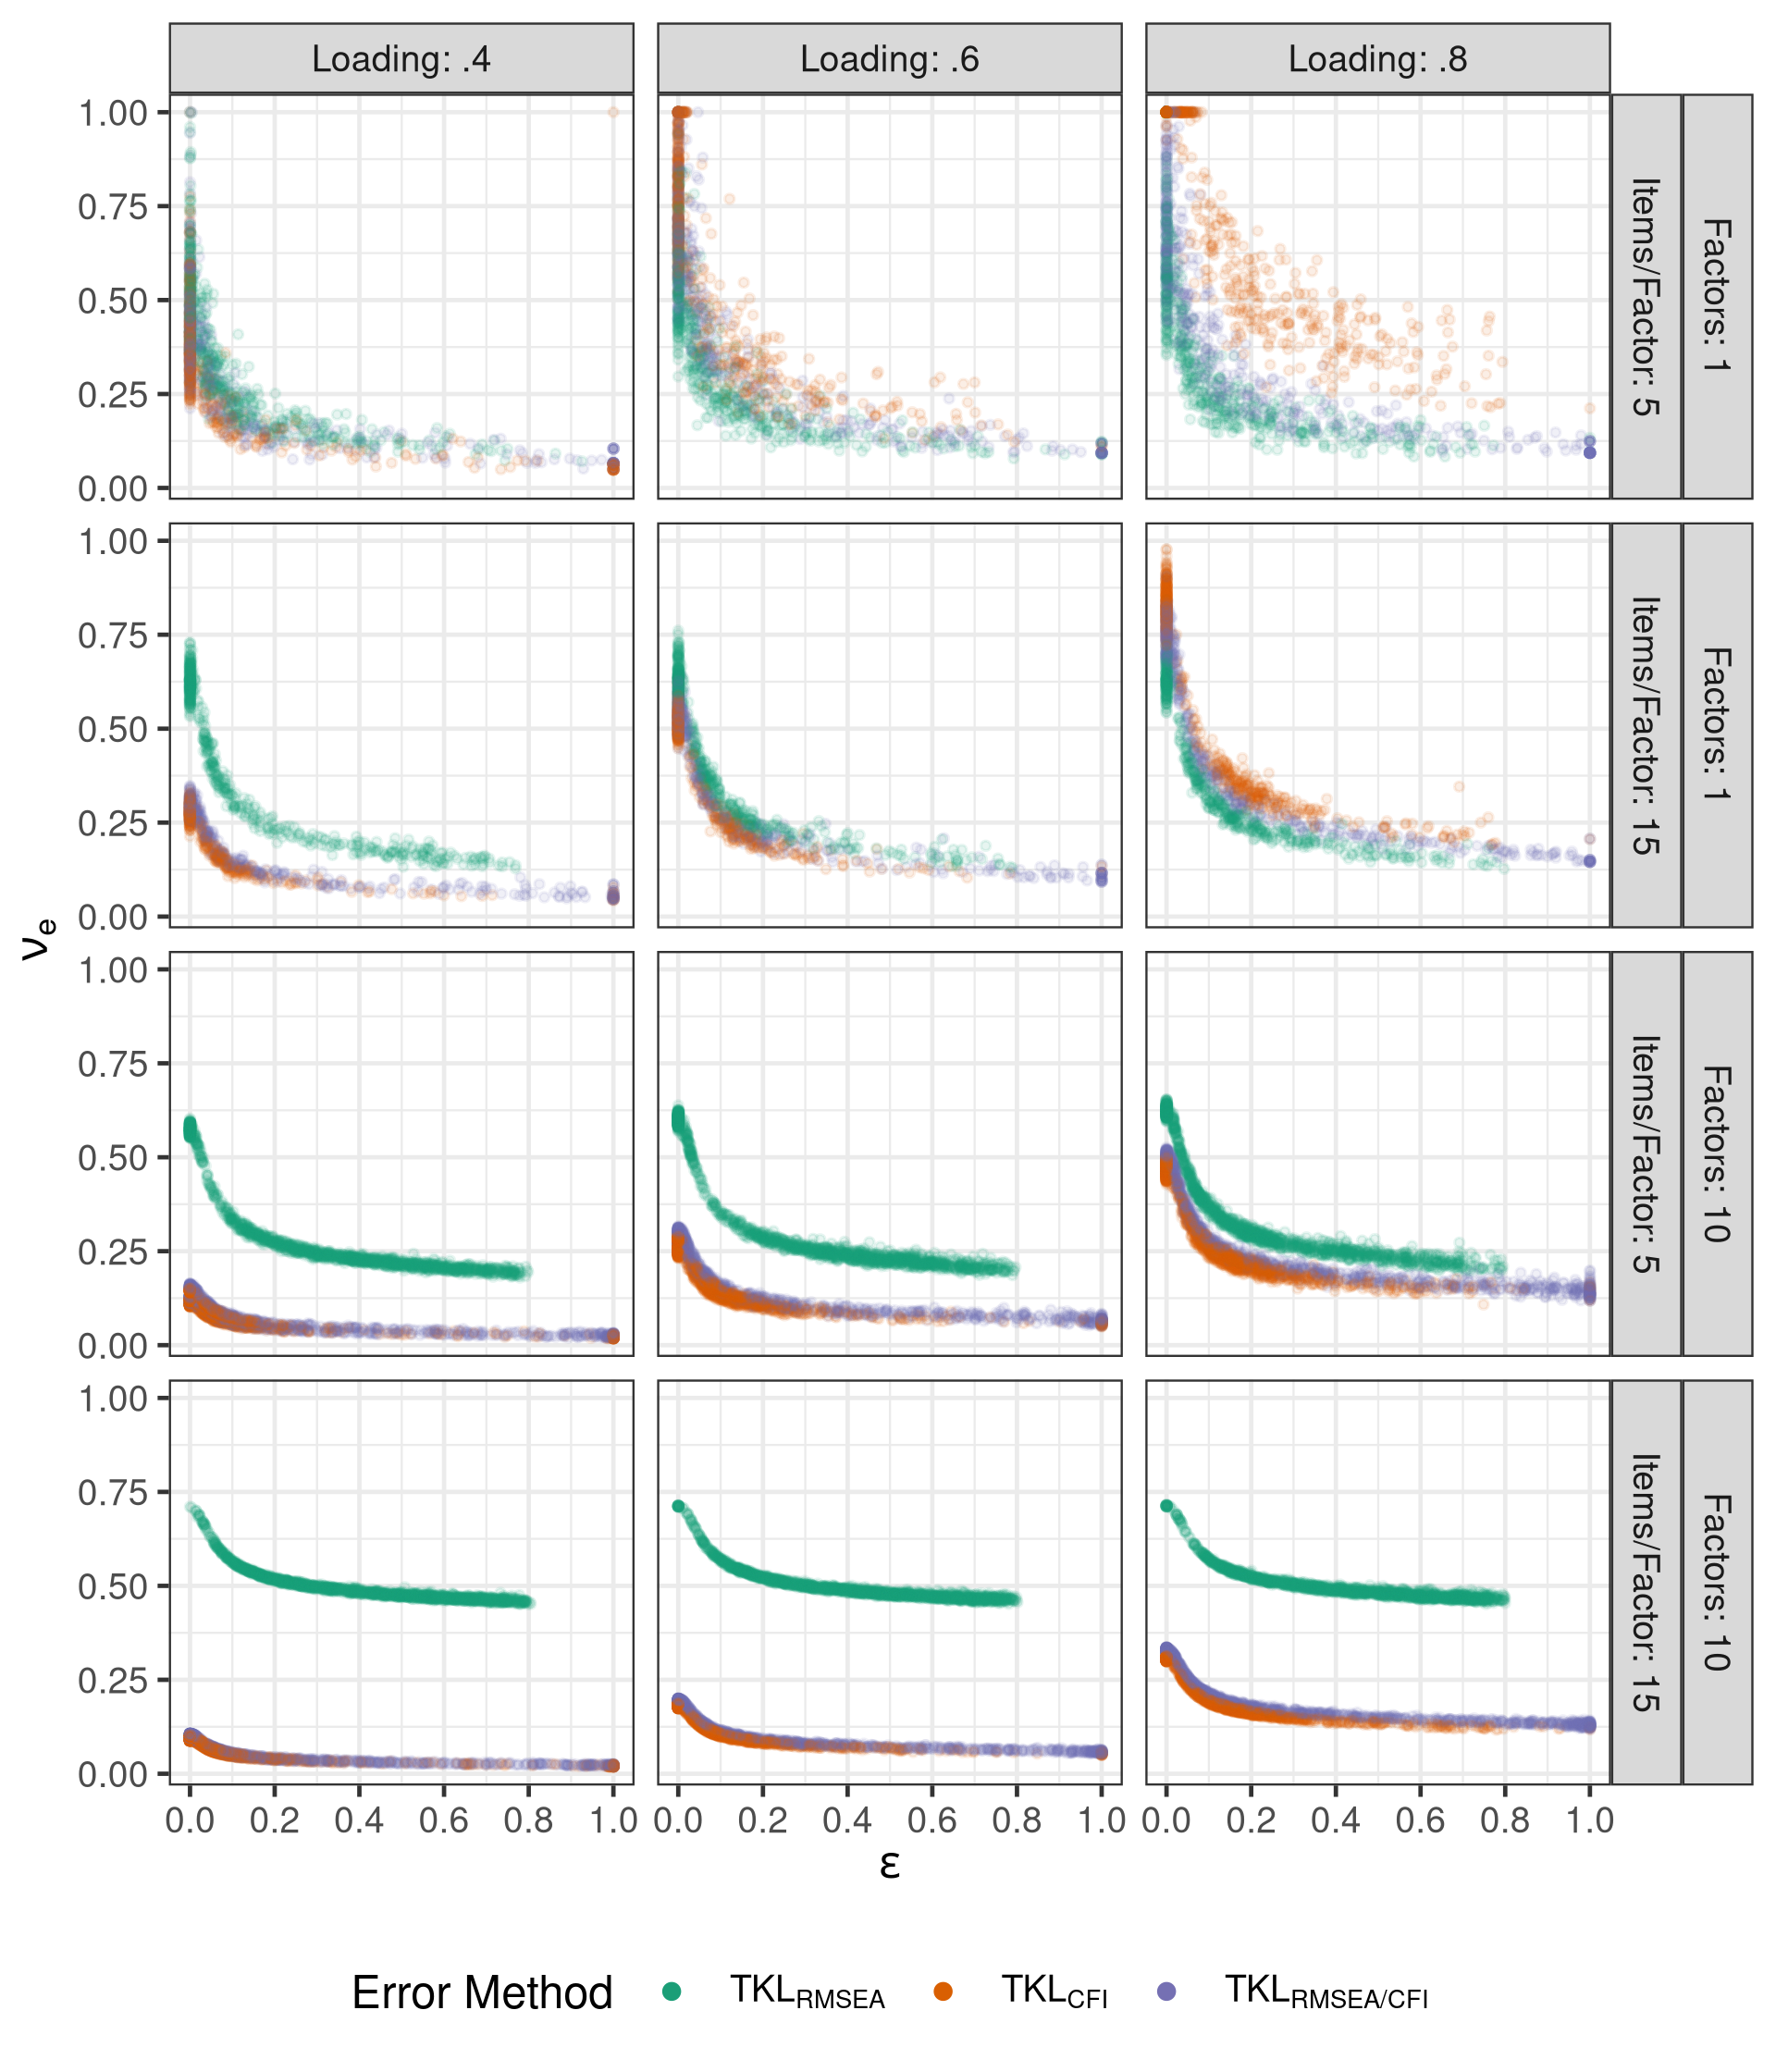
\includegraphics[width=0.8\linewidth]{img/eps_and_nu_w_violations} 

}

\caption[Values of the TKL parameters ($\epsilon$ and $\nu_{\textrm{e}}$) by model-error method, number of factors, number of items per factor, and factor loading strength when model fit was Poor]{Values of the TKL parameters ($\epsilon$ and $\nu_{\textrm{e}}$) by model-error method, number of factors, number of items per factor, and factor loading strength when model fit was Poor. Results for conditions with three or five major factors were omitted to conserve space. TKL = Tucker, Koopman, and Linn.}\label{fig:eps-and-v-values-by-W-violations}
\end{figure}

\begin{figure}

{\centering 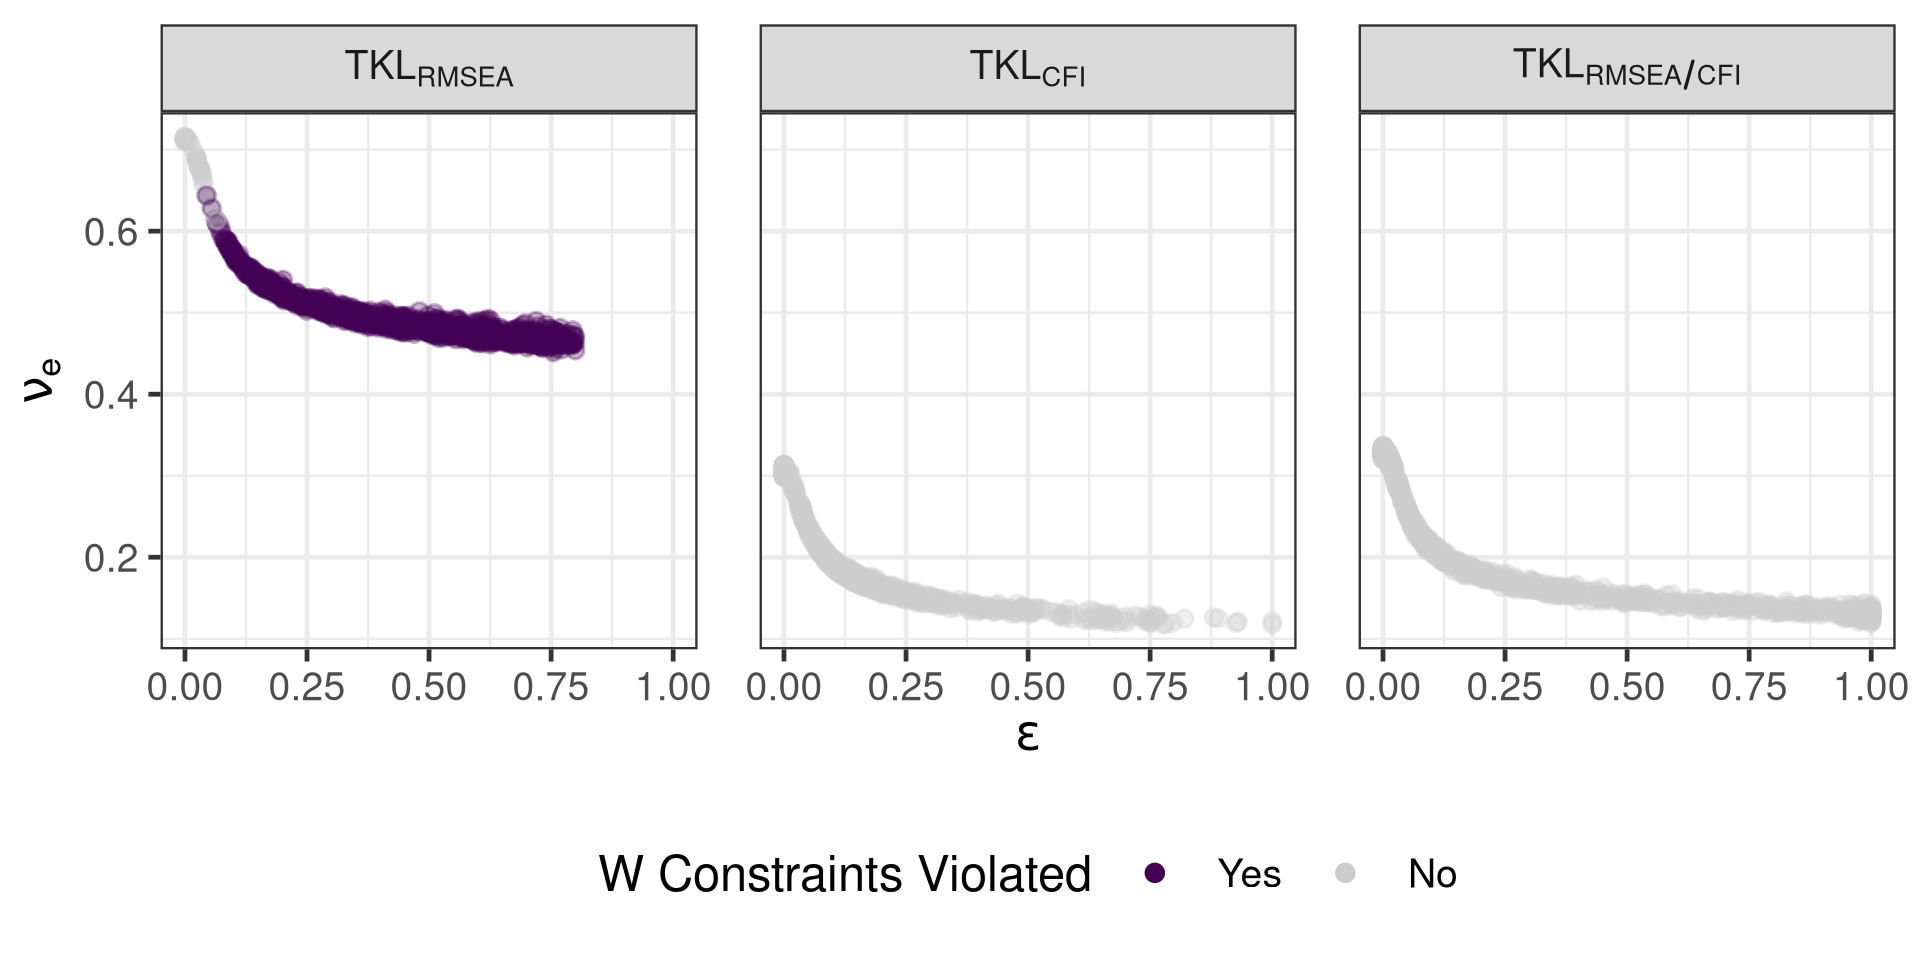
\includegraphics[width=0.8\linewidth]{img/eps_and_nu_violation_example} 

}

\caption[The distribution of $\epsilon$ and $\nu_{\textrm{e}}$ (and whether or not $\mathbf{W}$ constraints were violated) for conditions with Poor model fit, 10 factors, 15 items per factor, and factor loadings of .8]{The distribution of $\epsilon$ and $\nu_{\textrm{e}}$ (and whether or not $\mathbf{W}$ constraints were violated) for conditions with Poor model fit, 10 factors, 15 items per factor, and factor loadings of .8. TKL = Tucker, Koopman, and Linn}\label{fig:w-violation-example}
\end{figure}

\hypertarget{distributions-of-fit-statistics}{%
\section{Distributions of Fit Statistics}\label{distributions-of-fit-statistics}}

One of the primary questions the simulation study was intended to answer was whether the five model-error methods produced solutions with different fit index values when used with the same error-free models and target RMSEA and CFI values. In this section, I report the distributions of the RMSEA, CFI, TLI and CRMR model-fit indices for solutions produced by each of the five model-error methods (\(\textrm{TKL}_{\textrm{RMSEA}}\), \(\textrm{TKL}_{\textrm{CFI}}\), \(\textrm{TKL}_{\textrm{RMSEA/CFI}}\), CB, and WB).

\hypertarget{rmsea}{%
\subsection{RMSEA}\label{rmsea}}

Of the fit indices investigated in this study, the RMSEA value has been most often used as a measure of model fit when generating covariance or correlation matrices with model error. Figure \ref{fig:rmsea-distributions} shows box-plots summarizing the distributions of RMSEA values for each of the model-error methods, conditioned on number of factors, model fit, and factor loading strength. Notice that the \(\textrm{TKL}_{\textrm{RMSEA}}\) and CB methods almost always produced solutions with RMSEA values that were very close to the target RMSEA values. This result makes sense because both methods use optimization to produce solutions with RMSEA values close to a specified target. However, a somewhat unexpected result was that the CB method occasionally produced solutions with RMSEA values that were much higher or lower than the target value, particularly in conditions with ten major factors.

After the \(\textrm{TKL}_{\textrm{RMSEA}}\) and CB methods, Figure \ref{fig:rmsea-distributions} shows that the WB method was the next best model-error method in terms of producing solutions with RMSEA values close to the target values. In fact, the WB method produced solutions with median RMSEA values that were as close to the target values as those from \(\textrm{TKL}_{\textrm{RMSEA}}\) and CB solutions. However, the WB method also led to more variable RMSEA values, particularly in conditions with poor model fit and many factors.

The two methods that performed worst in terms of producing solutions with RMSEA values close to the targets were the \(\textrm{TKL}_{\textrm{RMSEA/CB}}\) and \(\textrm{TKL}_{\textrm{CB}}\) methods. Figure \ref{fig:rmsea-distributions} shows that these methods often led to RMSEA values that were lower than the target values, except when there were relatively few factors and strong factor loadings. The largest differences between the observed and target RMSEA values for the \(\textrm{TKL}_{\textrm{RMSEA/CB}}\) and \(\textrm{TKL}_{\textrm{CB}}\) methods occurred in conditions with poor model fit and relatively weak factor loadings (.3). In those conditions, both methods led to RMSEA values that were considerably lower than the target values.

\begin{figure}

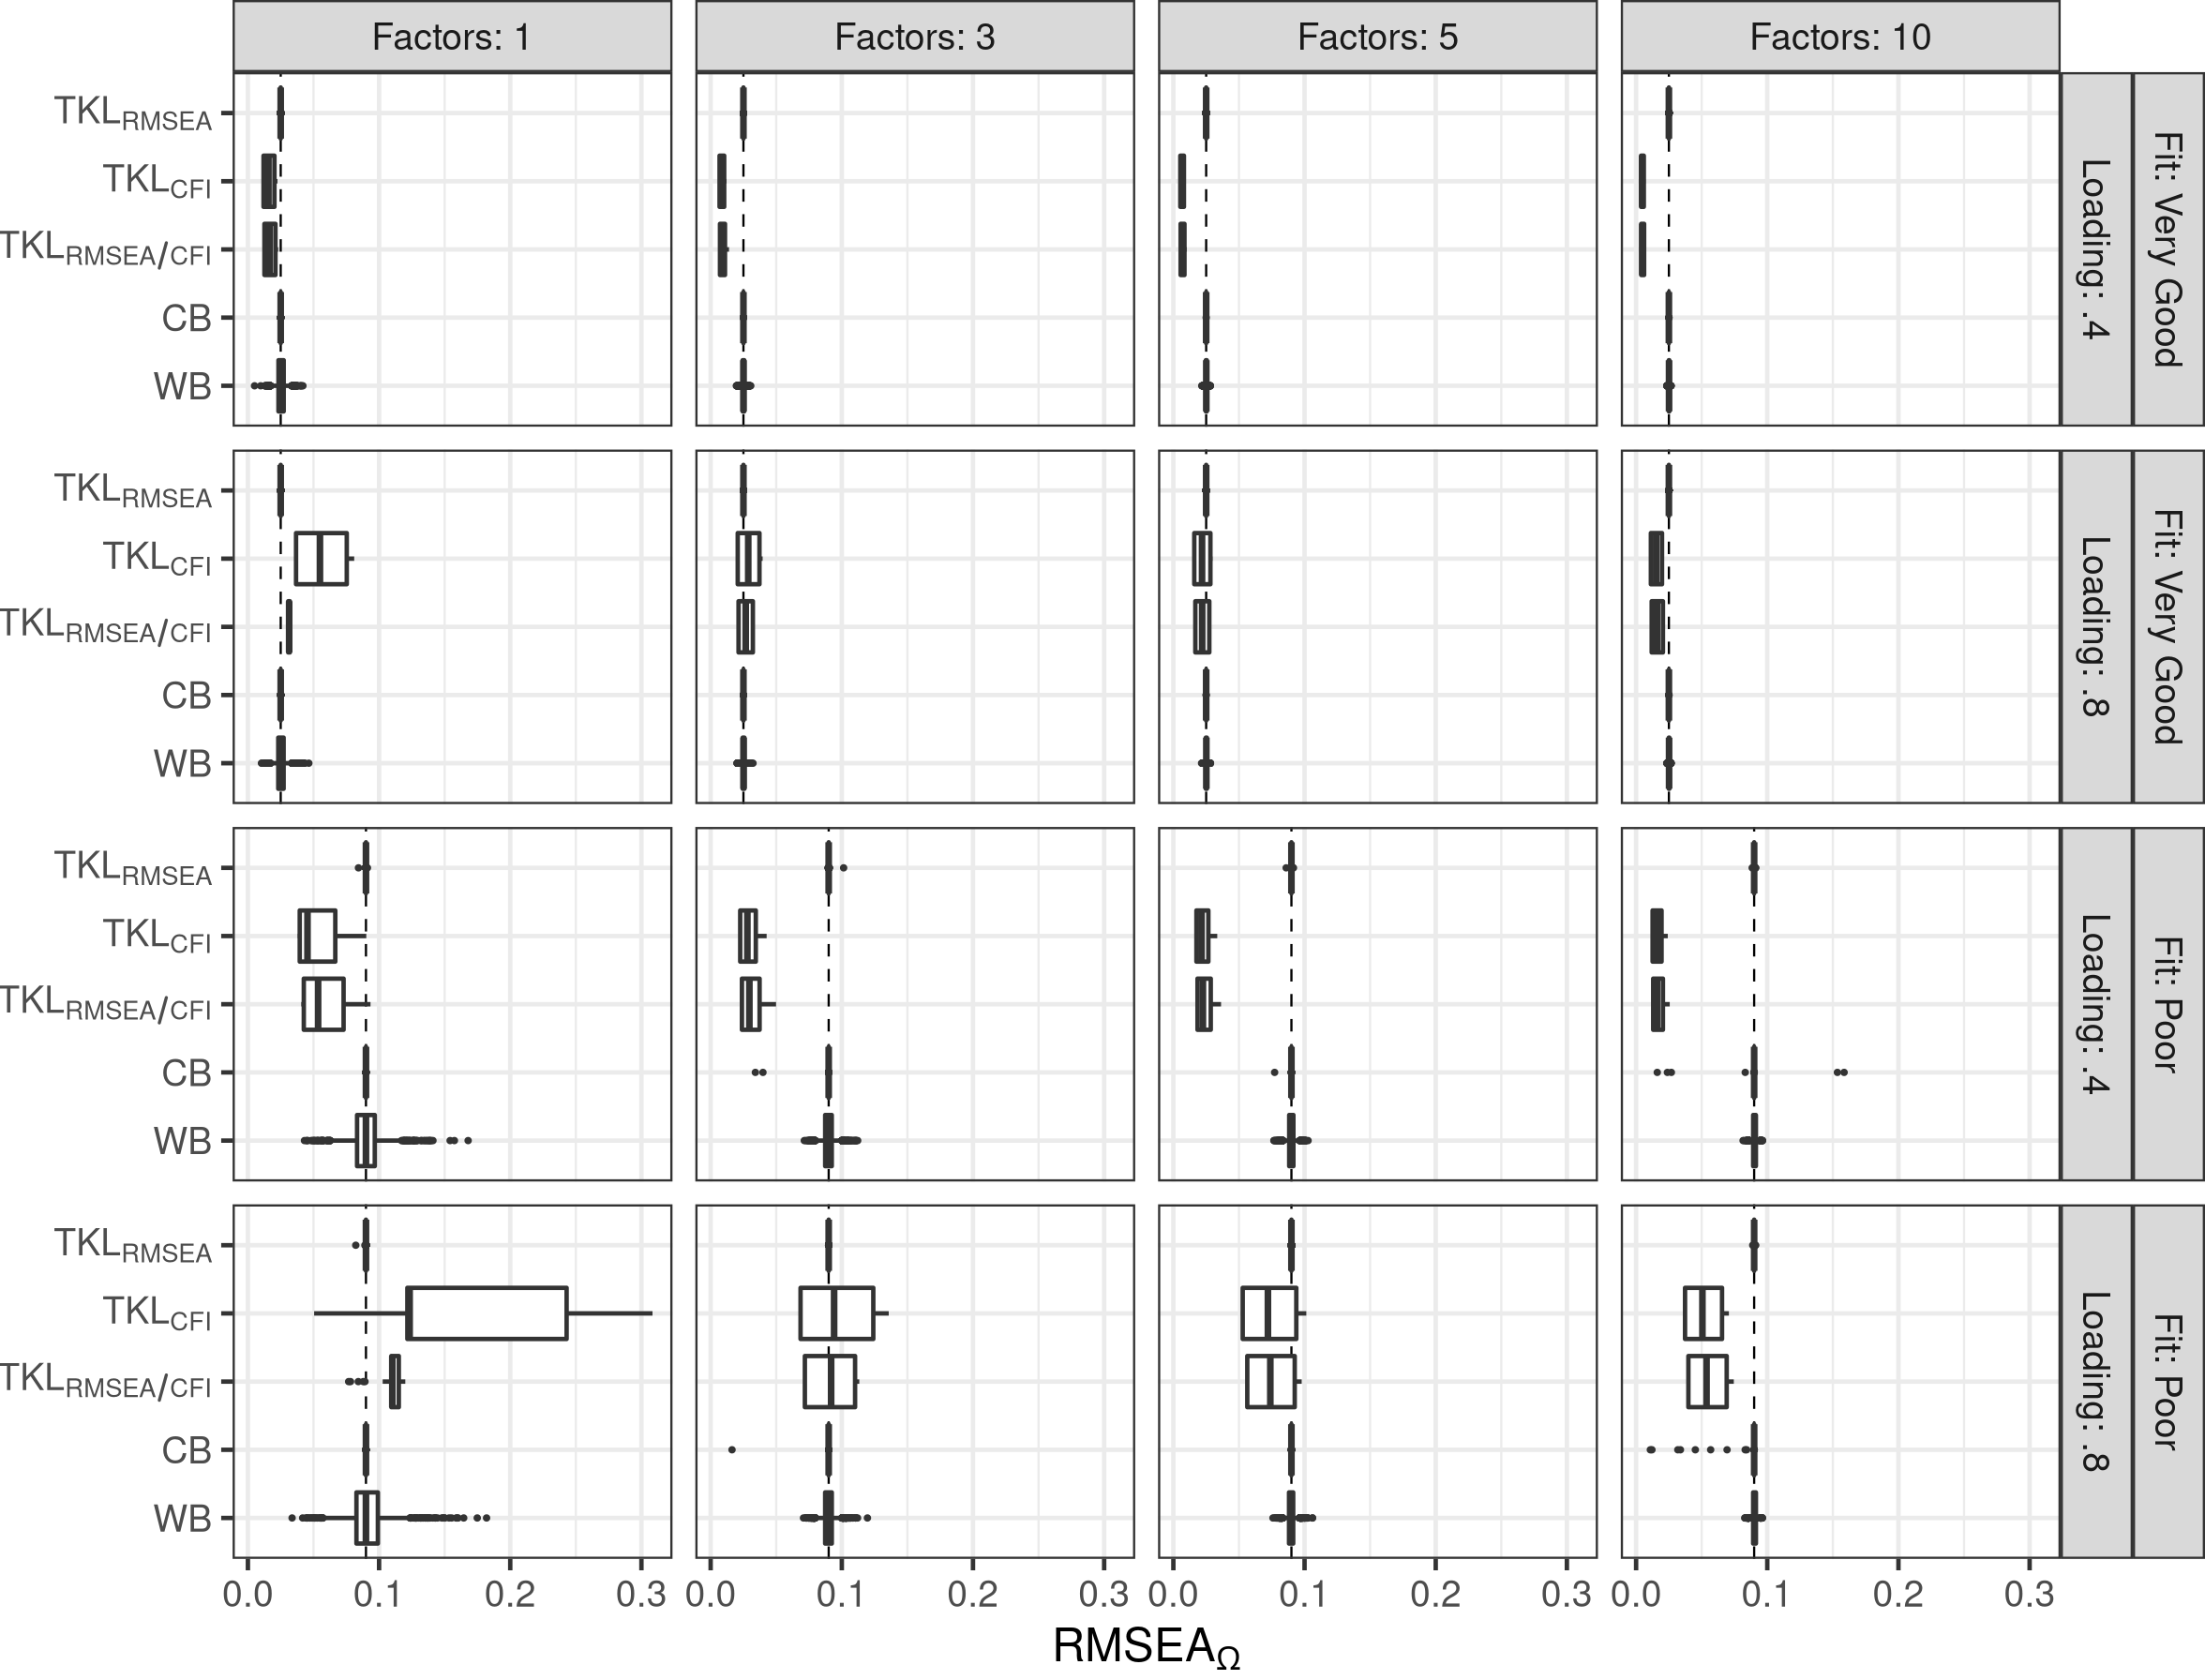
\includegraphics[width=425px]{/home/justin/Documents/dissertation/img/rmsea_distributions} \hfill{}

\caption[Distributions of the RMSEA values for solutions produced by each of the model-error methods, conditioned on number of factors, model fit, and factor loading strength]{Distributions of the RMSEA values for solutions produced by each of the model-error methods, conditioned on number of factors, model fit, and factor loading strength. The dashed lines indicate the target RMSEA value for each condition. Note that some levels of model fit and factor loading strength were omitted to conserve space. TKL = Tucker, Koopman, and Linn; CB = Cudeck and Browne; WB = Wu and Browne.}\label{fig:rmsea-distributions}
\end{figure}

\hypertarget{cfi}{%
\subsection{CFI}\label{cfi}}

{[}What are we doing for a transition here?{]} The distributions of CFI values for the solutions produced using the five model-error methods are shown in Figure \ref{fig:cfi-distributions}, conditioned on number of factors, model fit, and factor loading strength. As with \ref{fig:rmsea-distributions}, the middle levels of model fit and factor loading strength were omitted to converse space. Figure \ref{fig:cfi-distributions} shows that the results for CFI were nearly opposite to the results for RMSEA. Specifically, whereas the \(\textrm{TKL}_{\textrm{RMSEA}}\), CB, and WB methods produced solutions with RMSEA values much closer to the target values than those produced by the \(\textrm{TKL}_{\textrm{RMSEA/CFI}}\) or \(\textrm{TKL}_{\textrm{CFI}}\) methods, the \(\textrm{TKL}_{\textrm{RMSEA/CFI}}\) and \(\textrm{TKL}_{\textrm{CFI}}\) produced solutions with CFI values that were closer to the target CFI values compared to the other model-error methods in most conditions. The differences between the methods that optimized for CFI (\(\textrm{TKL}_{\textrm{RMSEA/CFI}}\) and \(\textrm{TKL}_{\textrm{CFI}}\)) and the other model-error methods were largest for conditions with poor model fit, poor factor loadings, and many factors (see the third row of Figure \ref{fig:cfi-distributions}). On the other hand, Figure \ref{fig:cfi-distributions} shows that all of the model-error methods produced similar CFI values (that were close to the target CFI value) for conditions with very good model fit and strong factor loadings.

A result in Figure \ref{fig:cfi-distributions} that is worth highlighting is that the \(\textrm{TKL}_{\textrm{RMSEA/CFI}}\) and \(\textrm{TKL}_{\textrm{CFI}}\) produced solutions with very similar CFI values in most conditions. These two methods also produced solutions with very similar RMSEA values in many conditions, as shown in Figure \ref{fig:rmsea-distributions}. Indeed, the \(\textrm{TKL}_{\textrm{RMSEA/CFI}}\) and \(\textrm{TKL}_{\textrm{CFI}}\) methods led to much more similar results in terms of both RMSEA and CFI than the \(\textrm{TKL}_{\textrm{RMSEA/CFI}}\) and \(\textrm{TKL}_{\textrm{RMSEA}}\) methods. Put another way, optimizing for CFI alone generally led to similar results compared to optimizing for both CFI and RMSEA, whereas optimizing for RMSEA alone generally led to solutions with much different RMSEA and CFI values compared to optimizing for both CFI and RMSEA. This suggests that CFI was more sensitive to small changes in parameter values than RMSEA.

The distributions of CFI values shown in Figure \ref{fig:cfi-distributions} also emphasize the importance of reporting multiple fit indices when simulating correlation or covariance matrices with model error. For instance, the \(\textrm{TKL}_{\textrm{RMSEA}}\) and CB methods produced solutions with RMSEA values close to the target RMSEA value of .09 in conditions with poor model fit and weak factor loadings. However, Figure \ref{fig:cfi-distributions} shows that those two model-error methods led to solutions with unacceptably low CFI values in the same conditions.

\begin{figure}

{\centering 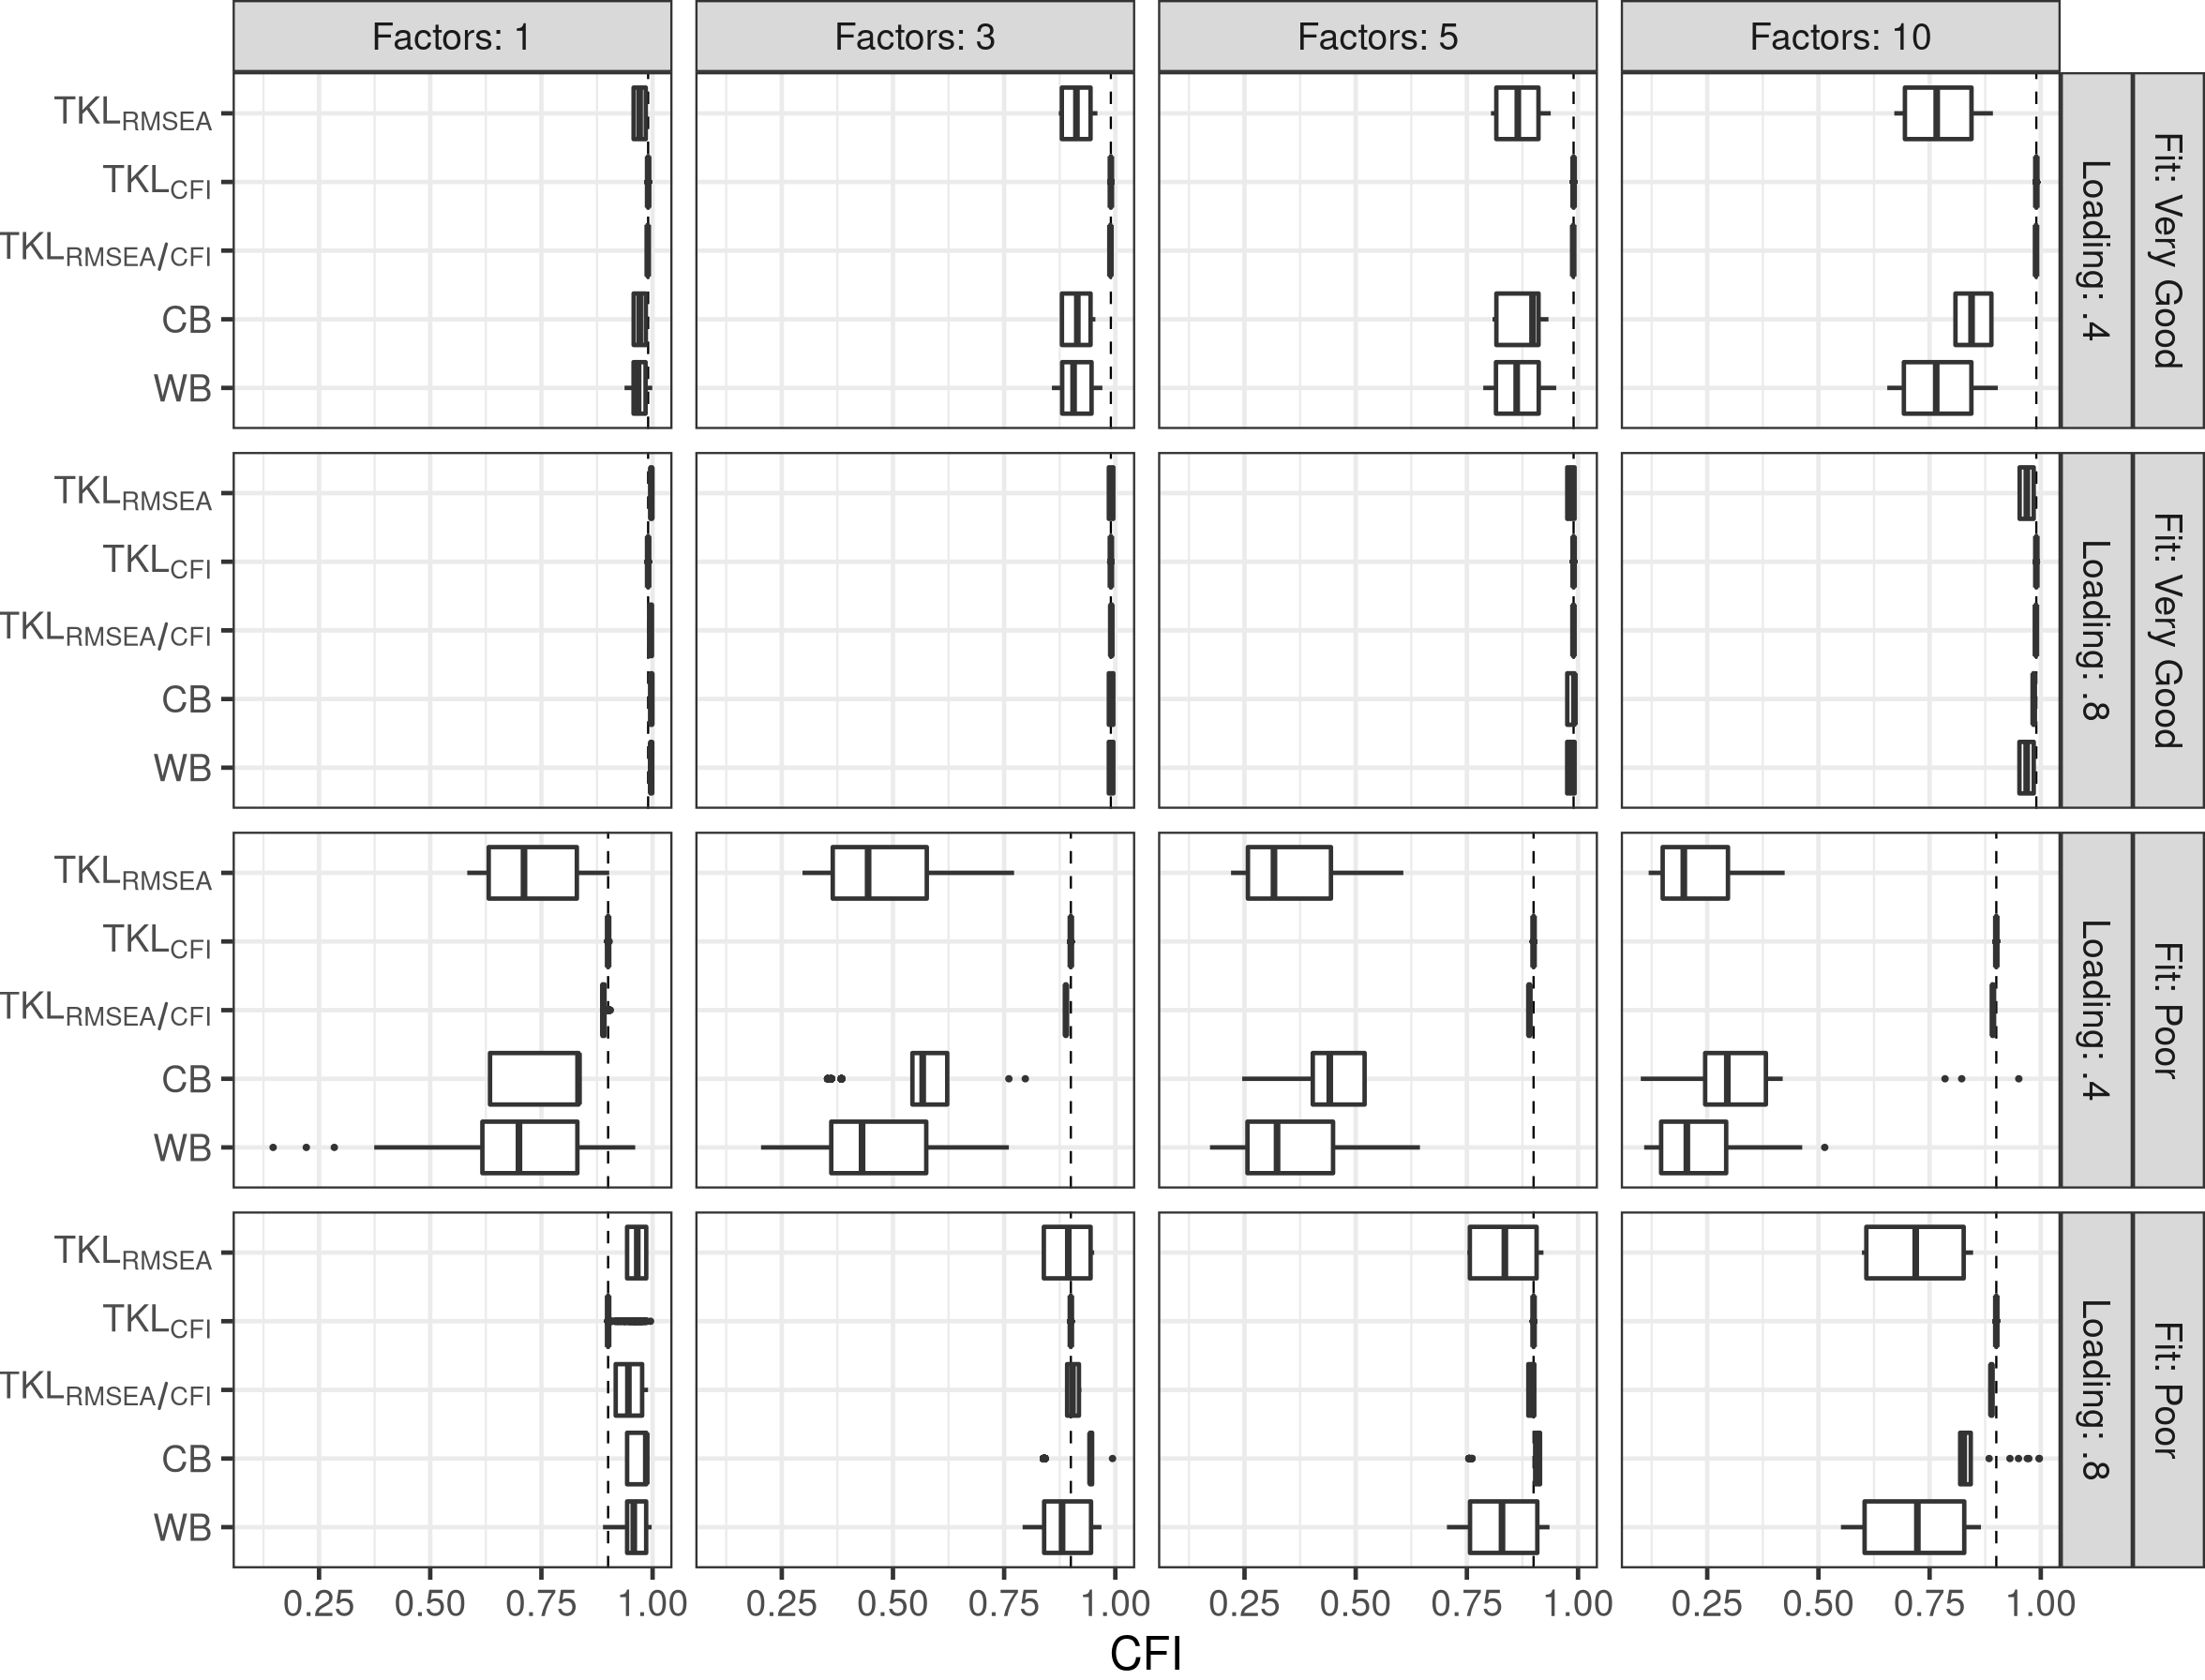
\includegraphics[width=425px]{/home/justin/Documents/dissertation/img/cfi_distributions} 

}

\caption[Distributions of the CFI values for solutions produced by each of the model-error methods, conditioned on number of factors, model fit, and factor loading strength]{Distributions of the CFI values for solutions produced by each of the model-error methods, conditioned on number of factors, model fit, and factor loading strength. The dashed lines indicate the target CFI value for each condition. Note that some levels of model fit and factor loading strength were omitted to conserve space. TKL = Tucker, Koopman, and Linn; CB = Cudeck and Browne; WB = Wu and Browne.}\label{fig:cfi-distributions}
\end{figure}

\hypertarget{tli}{%
\subsection{TLI}\label{tli}}

The distributions of TLI values for the solutions produced using the five model-error methods are shown in Figure \ref{fig:tli-distributions}, conditioned on number of factors, model fit, and factor loading strength. Overall, the distributions of TLI values were quite similar to the distributions of CFI values shown in Figure \ref{fig:cfi-distributions}. In particular, the \(\textrm{TKL}_{\textrm{CFI}}\) and \(\textrm{TKL}_{\textrm{RMSEA/CFI}}\) methods tended to produce solutions with higher TLI values than the other model-error methods, except for conditions with a single factor, Poor model fit, and strong factor loadings.

\begin{figure}

{\centering 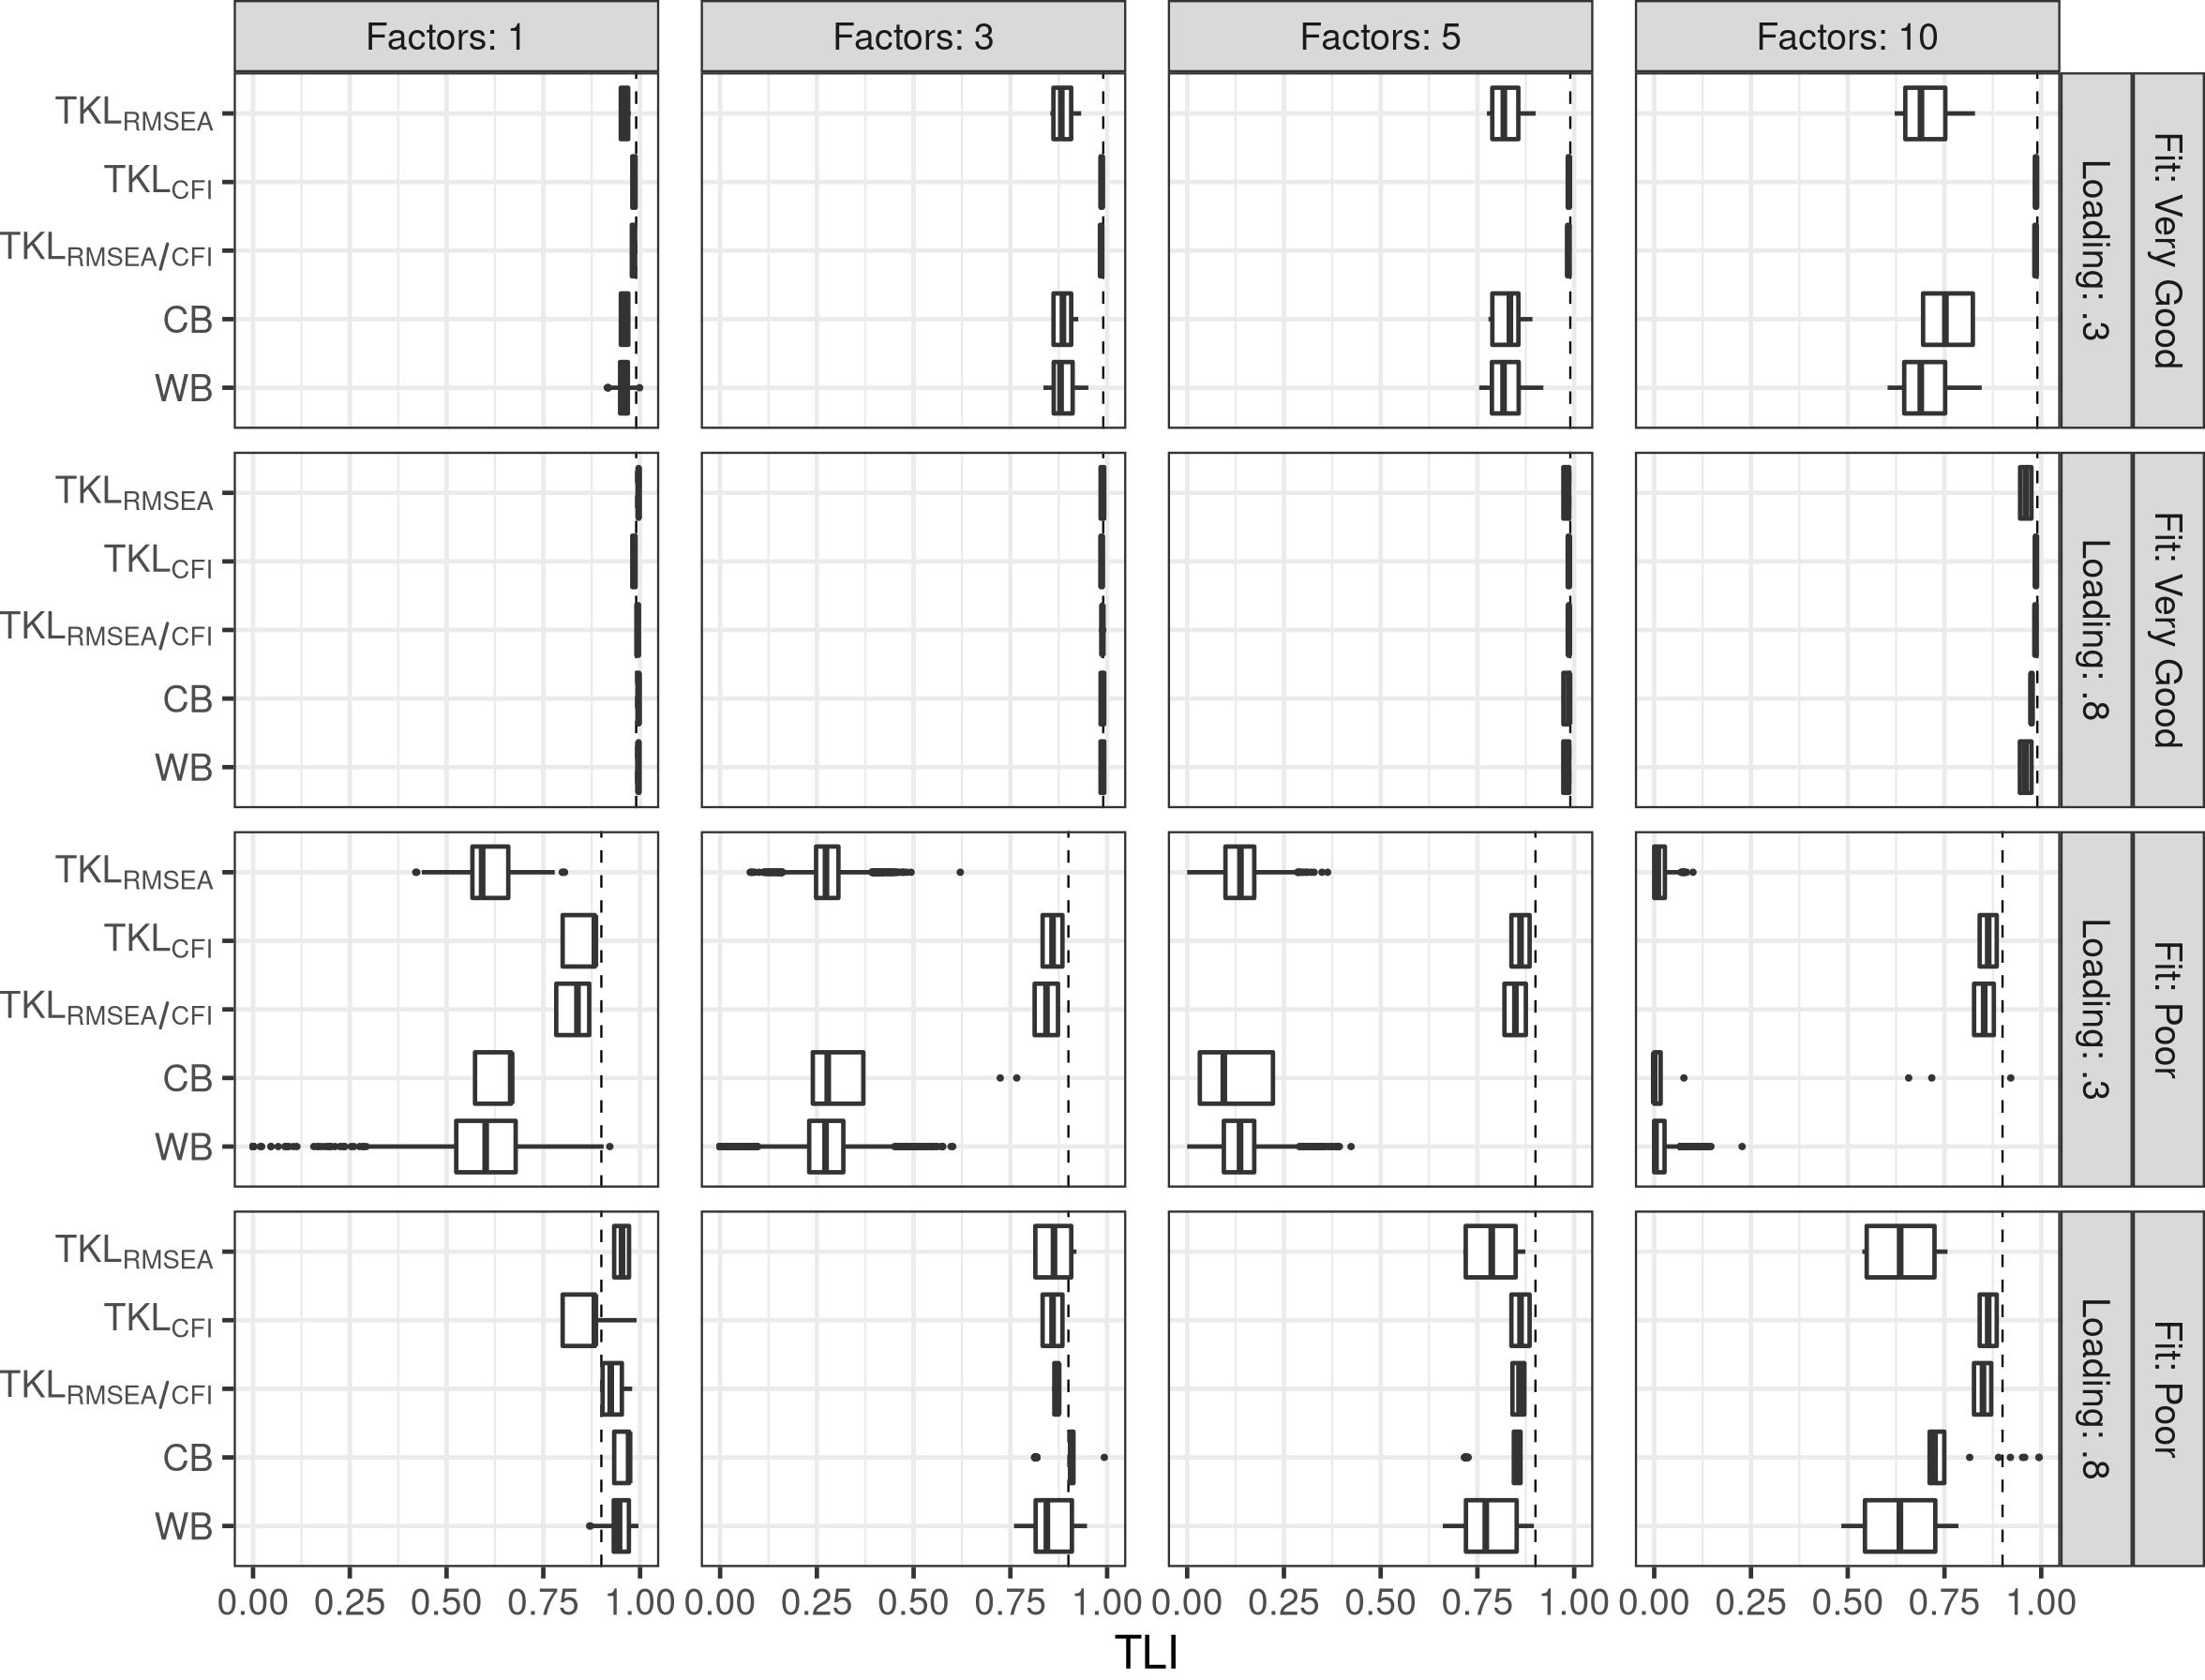
\includegraphics[width=1\linewidth]{/home/justin/Documents/dissertation/img/tli_distributions} 

}

\caption[Distributions of the TLI values for solutions produced by each of the model-error methods, conditioned on number of factors, model fit, and factor loading strength]{Distributions of the TLI values for solutions produced by each of the model-error methods, conditioned on number of factors, model fit, and factor loading strength. The dashed lines indicate the threshold values of TLI that correspond to the targeted levels of model fit, according to Hu and Bentler (1999). Note that some levels of model fit and factor loading strength were omitted to conserve space. TKL = Tucker, Koopman, and Linn; CB = Cudeck and Browne; WB = Wu and Browne.}\label{fig:tli-distributions}
\end{figure}

Similar to CFI, the differences in TLI values resulting from the \(\textrm{TKL}_{\textrm{CFI}}\) and \(\textrm{TKL}_{\textrm{RMSEA/CFI}}\) methods compared to the other model-error methods were most pronounced for conditions with many factors, weak factor loadings, and Poor model fit. This result (and the similar result for CFI) can be understood by thinking about how the relative and absolute fit indices differ in how they describe model fit. As an example, consider the an orthogonal model with ten major factors, five items per factor, and major common factor loadings fixed at .4. The population correlation matrix without model error for this condition (\(\bm{\Omega}\)) was \(50 \times 50\) block-diagonal correlation matrix, with correlations of \(0.16\) between items that load on the same factor and zero otherwise. To obtain a population correlation matrix (\(\bm{\Sigma}\)) with sufficient model error to indicate poor model fit (based on an RMSEA value of 0.09), the elements of the \(\mathbf{W}\) matrix had to be large enough to ensure that the square average squared difference between the off-diagonal elements of \(\bm{\Omega}\) and \(\bm{\Sigma}\) was 0.0081. Because the ``noise'' correlations from the minor common factors were relatively large compared to the non-zero elements of \(\bm{\Omega}\), the \(\bm{\Sigma}\) matrix did not have a clear factor structure. Thus, the major-factor model did not fit the \(\bm{\Sigma}\) very well because the model was unable to account for the correlations between the items represented in the off-block-diagonal elements of \(\bm{\Sigma}\) that were introduced by the \(\mathbf{WW}^\prime\) matrix. Moreover, because the \(\mathbf{WW}^\prime\) matrix increased the correlations between nearly all of the items that were uncorrelated in \(\bm{\Omega}\), the independence model used as a baseline for computing CFI fit \(\bm{\Sigma}\) relatively well.

\begin{figure}

{\centering 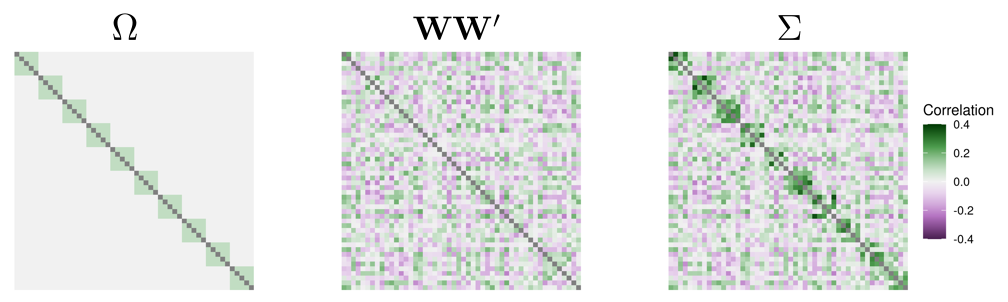
\includegraphics[width=1\linewidth]{/home/justin/Documents/dissertation/img/omega_plus_WtW_with_annotations} 

}

\caption[The population correlation matrix without model error ($\bm{\Sigma}$), the matrix of item correlations due to the minor common factors ($\mathbf{WW}^\prime$), and the population matrix with model error ($\bm{\Sigma}$) for an orthogonal model with ten major factors, five items per factor, and major common factor loadings fixed at .4]{The population correlation matrix without model error ($\bm{\Sigma}$), the matrix of item correlations due to the minor common factors ($\mathbf{WW}^\prime$), and the population matrix with model error ($\bm{\Sigma}$) for an orthogonal model with ten major factors, five items per factor, and major common factor loadings fixed at .4. The RMSEA and CFI values for this example were 0.09 and 0.25.}\label{fig:omega-wtw-sigma-example}
\end{figure}

The effects of the model error introduced by the minor common factors can be seen in Figure \ref{fig:omega-wtw-sigma-example}, which contains visual representations of \(\bm{\Omega}\), \(\textrm{WW}^\prime\), and \(\bm{\Sigma}\) matrices. The \(\mathbf{W}\) and \(\bm{\Sigma}\) matrices shown in the figure were obtained using the \(\textrm{TKL}_{\textrm{RMSEA}}\) method with a target RMSEA value of 0.09. The observed RMSEA and CFI values for \(\bm{\Sigma}\) were 0.09 and 0.25. Notice in Figure \ref{fig:omega-wtw-sigma-example} how large the elements of the \(\mathbf{WW}^\prime\) matrix were relative to the \(\bm{\Omega}\) matrix and how many off-block-diagonal elements there were relative to the block diagonal elements. This helps explain the incompatibility between RMSEA and CFI for models with many factors, weak major common factor loadings, and target RMSEA and CFI values reflecting poor model fit. To get an RMSEA value in line with the target value, all of the elements of \(\bm{\Omega}\) were perturbed. The perturbations to the off-block-diagonal elements of \(\bm{\Omega}\) were important in terms of the resulting CFI value because they were incompatible with the major common factor model (i.e., they should have been zero under that model) and therefore degraded the fit of the major factor model for \(\bm{\Sigma}\) while improving the fit of the independence model. The effect of perturbing these off-block-diagonal elements became more pronounced as the number of factors increased because the number of off-block-diagonal elements increased faster than the number of block-diagonal elements as the total number of items increased. This can be clearly seen in Figure \ref{fig:off-diag-elements}, which shows the number of block diagonal elements and off-block-diagonal elements in the lower triangle of \(\bm{\Sigma}\) as the number of factors increased for an orthogonal model with five items per factor.

\begin{figure}

{\centering 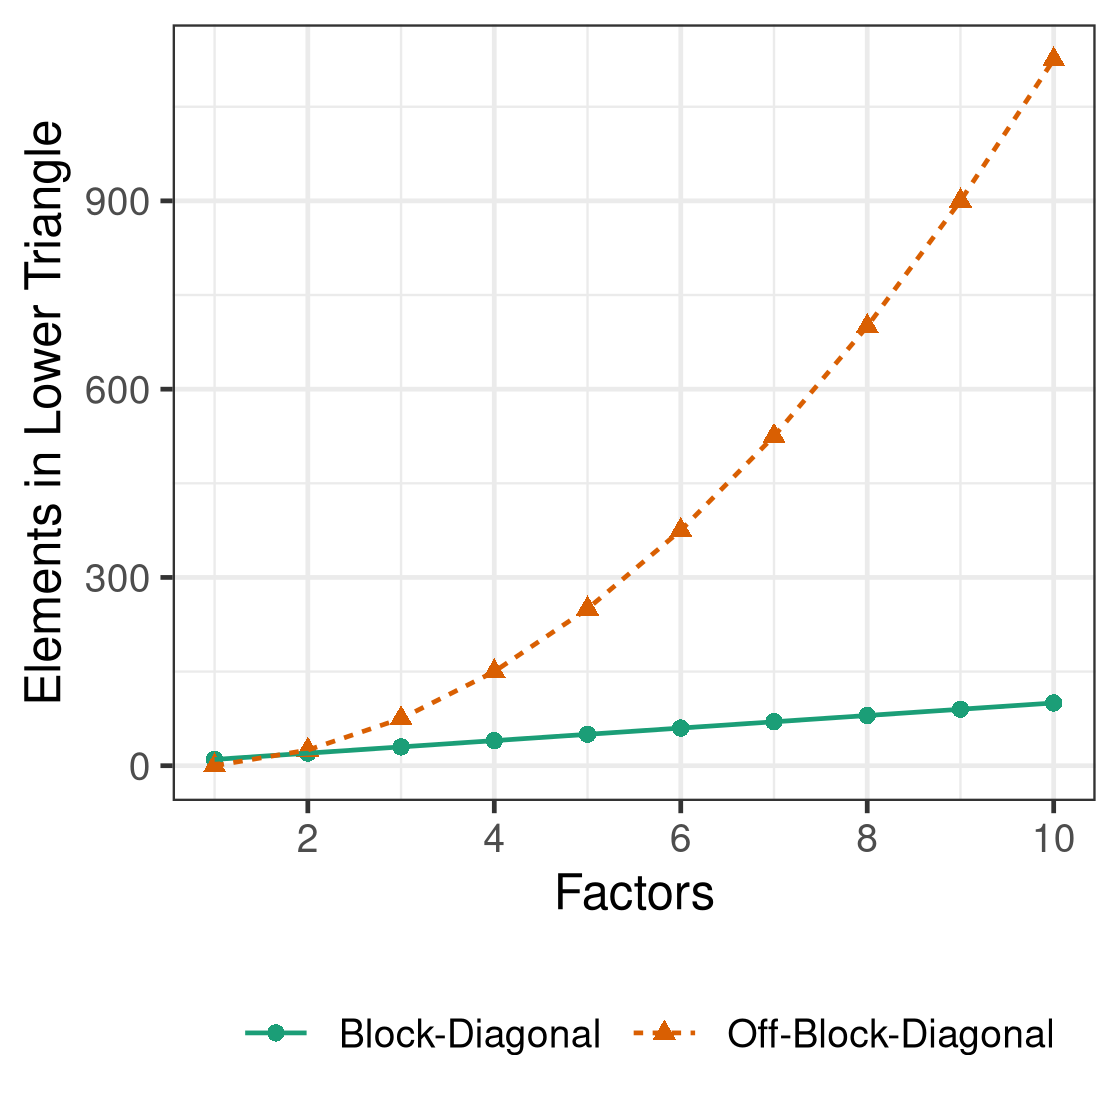
\includegraphics[width=0.8\linewidth]{/home/justin/Documents/dissertation/img/off-diagonal-elements} 

}

\caption[The number of block-diagonal elements in the lower-triangle of $\bm{\Sigma}$ compared to the number of off-block-diagonal elements for an orthogonal model with five items per factor]{The number of block-diagonal elements in the lower-triangle of $\bm{\Sigma}$ compared to the number of off-block-diagonal elements for an orthogonal model with five items per factor.}\label{fig:off-diag-elements}
\end{figure}

\hypertarget{crmr}{%
\subsection{CRMR}\label{crmr}}

Just as the TLI results were similar to the CFI results, the CRMR results were similar in many ways to the RMSEA results. In particular,

\begin{figure}

{\centering 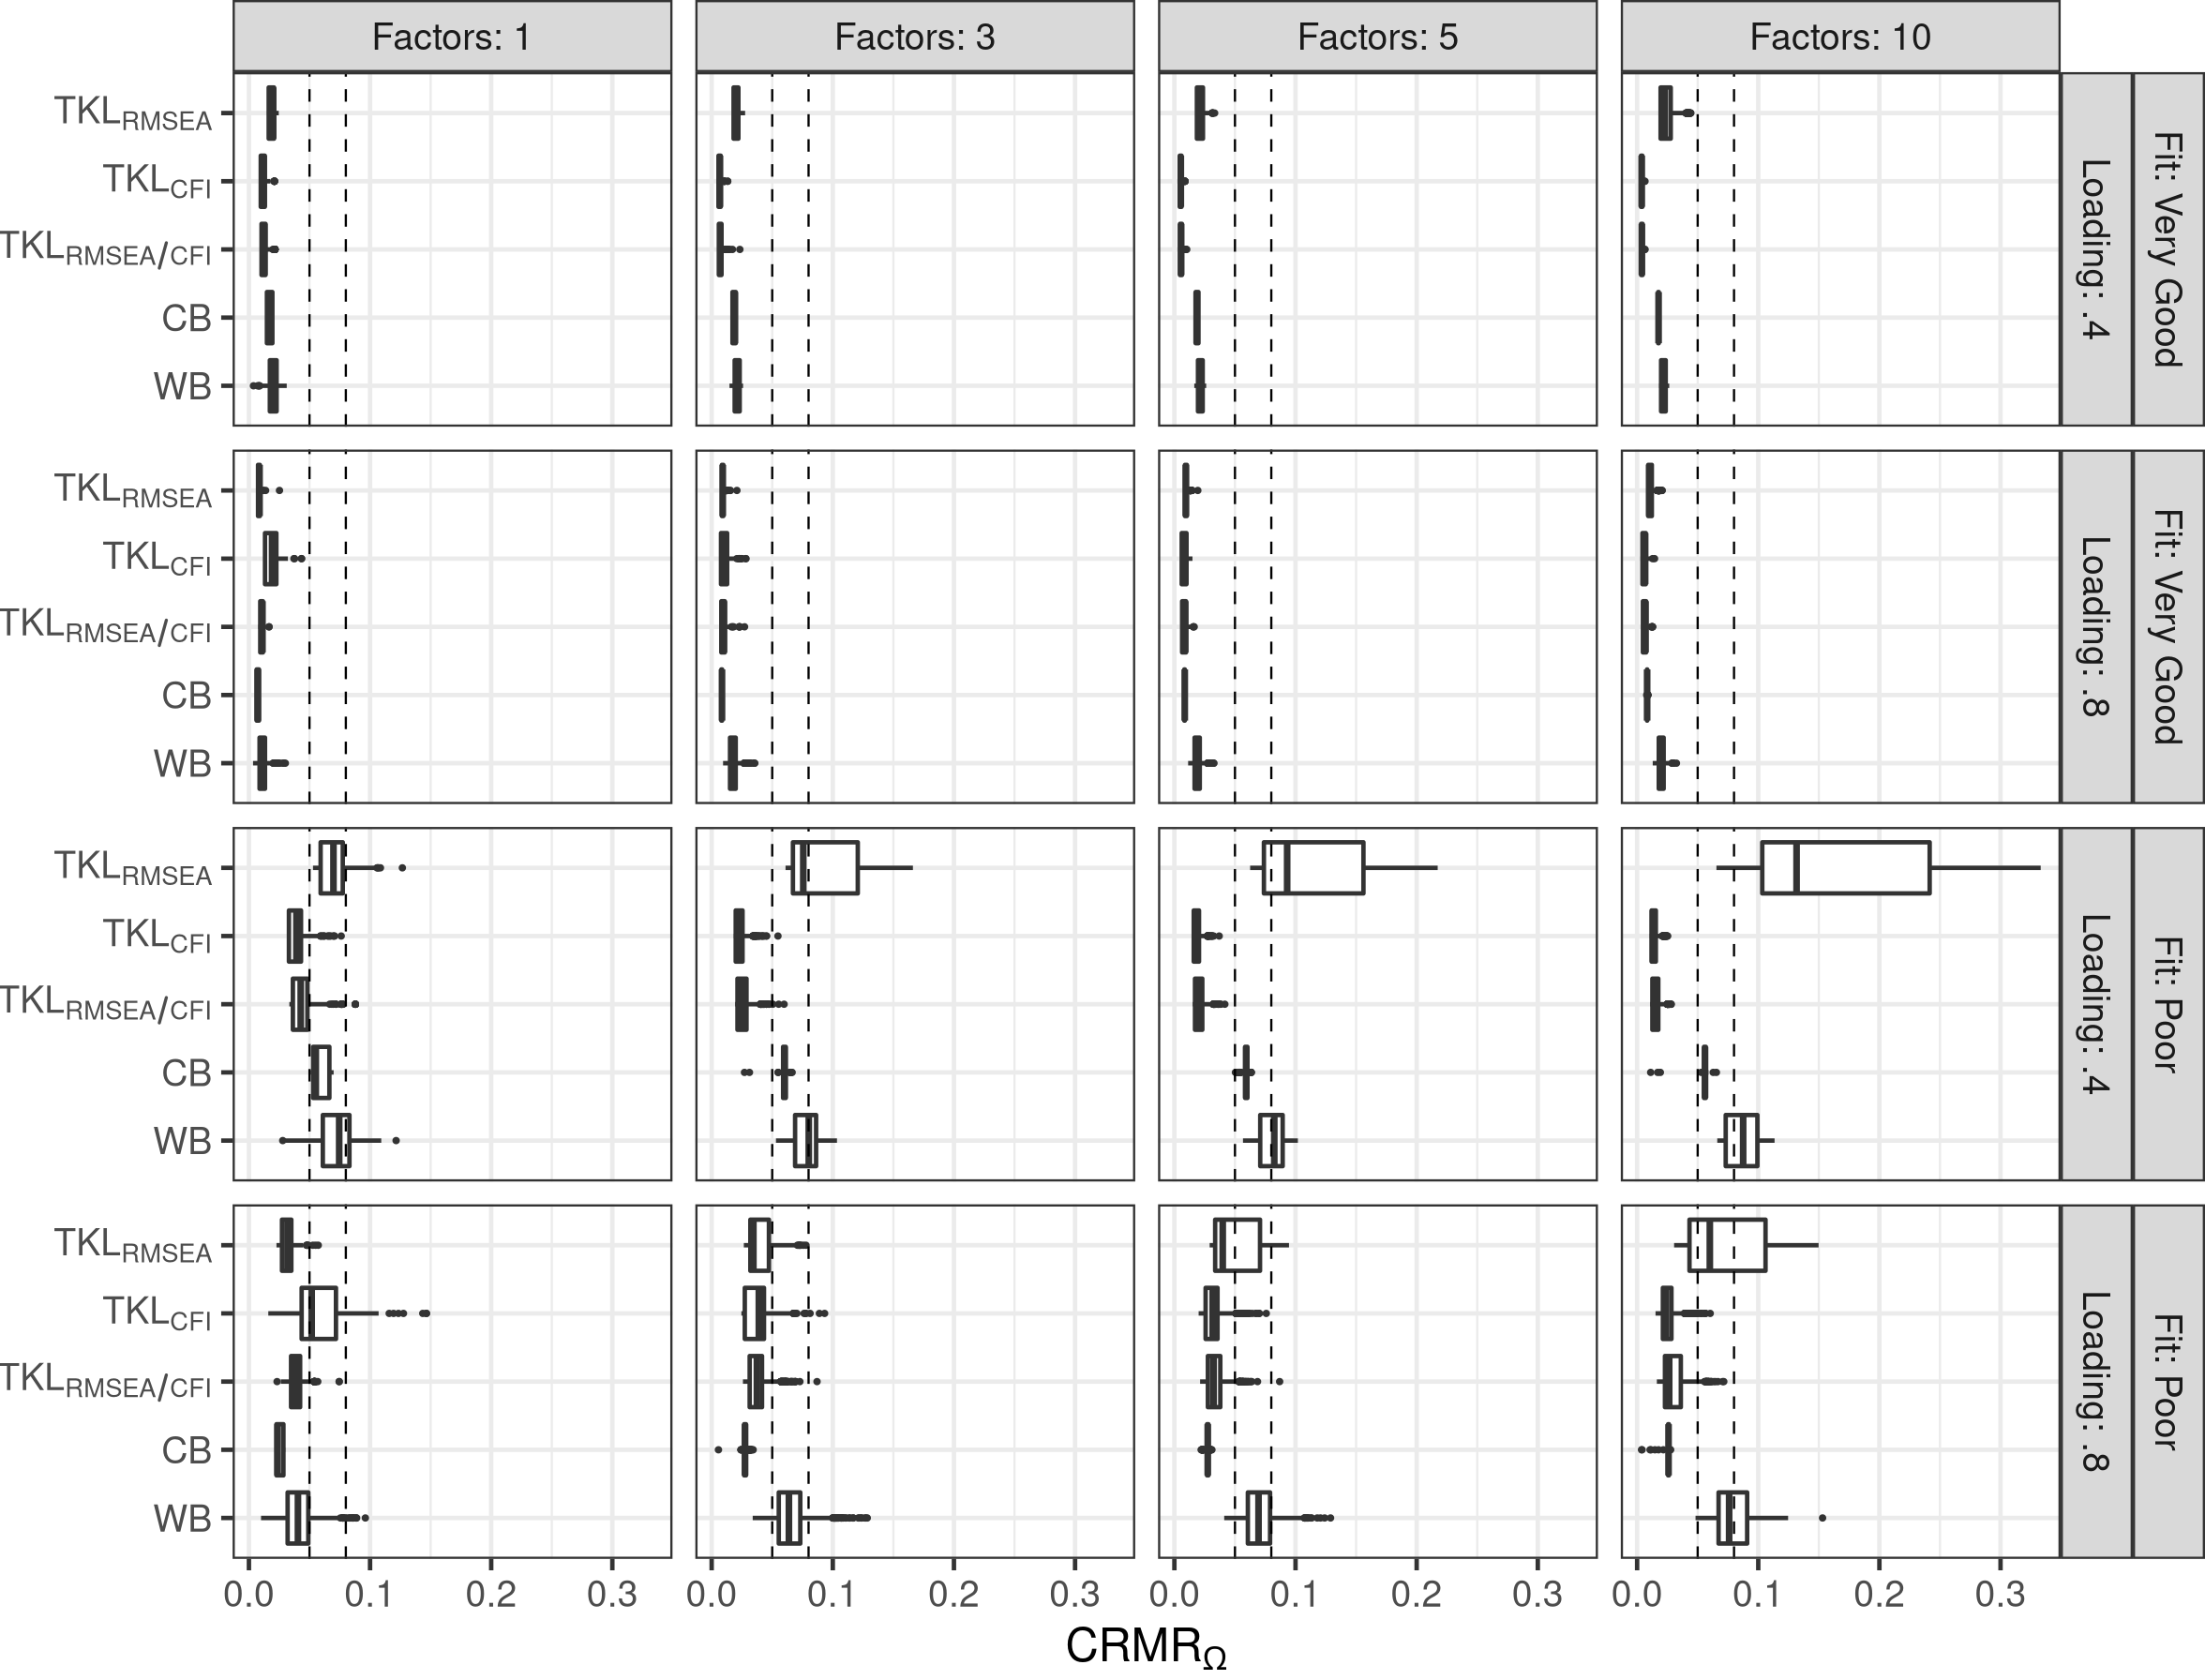
\includegraphics[width=1\linewidth]{/home/justin/Documents/dissertation/img/crmr_distributions} 

}

\caption[Distributions of the CRMR values for solutions produced by each of the model-error methods, conditioned on number of factors, model fit, and factor loading strength]{Distributions of the CRMR values for solutions produced by each of the model-error methods, conditioned on number of factors, model fit, and factor loading strength. The dashed lines indicate the threshold values of SRMR/CRMR that correspond to the targeted levels of model fit, according to Hu and Bentler (1999). Note that some levels of model fit and factor loading strength were omitted to conserve space. TKL = Tucker, Koopman, and Linn; CB = Cudeck and Browne; WB = Wu and Browne.}\label{fig:crmr-distributions}
\end{figure}

\hypertarget{discussion}{%
\chapter{Discussion}\label{discussion}}

Lorem ipsum dolor sit amet, consectetur adipiscing elit. Maecenas vel eros sed mauris porttitor semper nec a orci. Nullam vestibulum mi nec condimentum posuere. Pellentesque eget diam id sapien aliquet ullamcorper. Pellentesque blandit nec lectus ut mollis. Praesent in facilisis justo. Vestibulum ante ipsum primis in faucibus orci luctus et ultrices posuere cubilia Curae; Sed eget congue leo, sed consequat libero. In rutrum malesuada nisi. Vestibulum ante ipsum primis in faucibus orci luctus et ultrices posuere cubilia Curae; Morbi sollicitudin tortor ut sem facilisis mollis.

\hypertarget{references}{%
\chapter*{References}\label{references}}
\addcontentsline{toc}{chapter}{References}

\noindent

\setlength{\parindent}{-0.20in}
\setlength{\leftskip}{0.20in}
\setlength{\parskip}{8pt}

\hypertarget{refs}{}
\begin{CSLReferences}{1}{0}
\leavevmode\vadjust pre{\hypertarget{ref-beauducel2016}{}}%
Beauducel, A., \& Hilger, N. (2016). On the correlation of common factors with variance not accounted for by the factor model. \emph{Communications in Statistics - Simulation and Computation}, \emph{45}(6), 2145--2157. \url{https://doi.org/gh64s7}

\leavevmode\vadjust pre{\hypertarget{ref-bentler1990}{}}%
Bentler, P. M. (1990). Comparative fit indexes in structural models. \emph{Psychological Bulletin}, \emph{107}(2), 238--246. \url{https://doi.org/dbj}

\leavevmode\vadjust pre{\hypertarget{ref-bentler1980}{}}%
Bentler, P. M., \& Bonett, D. G. (1980). Significance tests and goodness of fit in the analysis of covariance structures. \emph{Psychological Bulletin}, \emph{88}(3), 588--606. \url{https://doi.org/dbm}

\leavevmode\vadjust pre{\hypertarget{ref-bezanson2017julia}{}}%
Bezanson, J., Edelman, A., Karpinski, S., \& Shah, V. B. (2017). Julia: {A} fresh approach to numerical computing. \emph{SIAM Review}, \emph{59}(1), 65--98. \url{https://doi.org/f9wkpj}

\leavevmode\vadjust pre{\hypertarget{ref-bollen1989}{}}%
Bollen, K. A. (1989). A new incremental fit index for general structural equation models. \emph{Sociological Methods \& Research}, \emph{17}(3), 303--316. \url{https://doi.org/cfgdt5}

\leavevmode\vadjust pre{\hypertarget{ref-bollen1989a}{}}%
Bollen, Kenneth A. (1989). \emph{Structural {Equations} with {Latent Variables}}. {John Wiley \& Sons, Inc.} \url{https://doi.org/10.1002/9781118619179}

\leavevmode\vadjust pre{\hypertarget{ref-borges1998}{}}%
Borges, J. L. (1998). On exactitude in science. In A. Hurley (Ed.), \emph{Collected fictions}. {New York:Viking}.

\leavevmode\vadjust pre{\hypertarget{ref-box1987}{}}%
Box, G. E. P., \& Draper, N. R. (1987). \emph{Empirical model-building and response surfaces.} (pp. xiv, 669). {John Wiley \& Sons}.

\leavevmode\vadjust pre{\hypertarget{ref-briggs2003}{}}%
Briggs, N. E., \& MacCallum, R. C. (2003). Recovery of weak common factors by maximum likelihood and ordinary least squares estimation. \emph{Multivariate Behavioral Research}, \emph{38}(1), 25--56. \url{https://doi.org/bgnz9w}

\leavevmode\vadjust pre{\hypertarget{ref-browne1984}{}}%
Browne, M. W. (1984). Asymptotically distribution-free methods for the analysis of covariance structures. \emph{British Journal of Mathematical and Statistical Psychology}, \emph{37}(1), 62--83. \url{https://doi.org/cd4vn7}

\leavevmode\vadjust pre{\hypertarget{ref-browne1992}{}}%
Browne, M. W., \& Cudeck, R. (1992). Alternative ways of assessing model fit. \emph{Sociological Methods \& Research}, \emph{21}(2), 230--258. \url{https://doi.org/dbn}

\leavevmode\vadjust pre{\hypertarget{ref-browne2002}{}}%
Browne, M. W., MacCallum, R. C., Kim, C. T., Andersen, B. L., \& Glaser, R. (2002). When fit indices and residuals are incompatible. \emph{Psychological Methods}, \emph{7}(4), 403--421. \url{https://doi.org/fhq5t3}

\leavevmode\vadjust pre{\hypertarget{ref-browne1988}{}}%
Browne, M. W., \& Shapiro, A. (1988). Robustness of normal theory methods in the analysis of linear latent variate models. \emph{British Journal of Mathematical and Statistical Psychology}, \emph{41}(2), 193--208. \url{https://doi.org/bdk8xk}

\leavevmode\vadjust pre{\hypertarget{ref-byrd1995}{}}%
Byrd, R. H., Lu, P., Nocedal, J., \& Zhu, C. (1995). A limited memory algorithm for bound constrained optimization. \emph{SIAM Journal on Scientific Computing}, \emph{16}(5), 1190--1208. \url{https://doi.org/bpjm24}

\leavevmode\vadjust pre{\hypertarget{ref-carroll1894}{}}%
Carroll, L. (1894). \emph{Sylvie and {Bruno}, {Volume II}, by {Lewis Carroll}, illustrated by {Harry Furniss}}. https://www.gutenberg.org/files/48795/48795-h/48795-h.htm.

\leavevmode\vadjust pre{\hypertarget{ref-chung2019}{}}%
Chung, S., \& Cai, L. (2019). Alternative multiple imputation inference for categorical structural equation modeling. \emph{Multivariate Behavioral Research}, \emph{54}(3), 323--337. \url{https://doi.org/gh64rk}

\leavevmode\vadjust pre{\hypertarget{ref-cudeck1989}{}}%
Cudeck, R. (1989). Analysis of correlation matrices using covariance structure models. \emph{Psychological Bulletin}, \emph{105}(2), 317--327. \url{https://doi.org/fqks6n}

\leavevmode\vadjust pre{\hypertarget{ref-cudeck1992}{}}%
Cudeck, R., \& Browne, M. W. (1992). Constructing a covariance matrix that yields a specified minimizer and a specified minimum discrepancy function value. \emph{Psychometrika}, \emph{57}(3), 357--369. \url{https://doi.org/cq6ckd}

\leavevmode\vadjust pre{\hypertarget{ref-cudeck1991}{}}%
Cudeck, R., \& Henly, S. J. (1991). Model selection in covariance structures analysis and the {``problem''} of sample size: {A} clarification. \emph{Psychological Bulletin}, \emph{109}(3), 512. \url{https://doi.org/bpqvdv}

\leavevmode\vadjust pre{\hypertarget{ref-dewinter2016}{}}%
de Winter, J. C. F., \& Dodou, D. (2016). Common factor analysis versus principal component analysis: {A} comparison of loadings by means of simulations. \emph{Communications in Statistics - Simulation and Computation}, \emph{45}(1), 299--321. \url{https://doi.org/gh64cn}

\leavevmode\vadjust pre{\hypertarget{ref-eco1994}{}}%
Eco, U. (1994). On the impossibility of drawing a map of the empire on a scale of 1 to 1. In W. Weaver \& U. Eco (Eds.), \emph{How to travel with a salmon \& other essays} (1st ed..). {New York:Harcourt, Brace}.

\leavevmode\vadjust pre{\hypertarget{ref-gelman2008}{}}%
Gelman, A. (2008). Some thoughts on the saying, {``{All} models are wrong, but some are useful.''} In \emph{Statistical Modeling, Causal Inference, and Social Science}. https://statmodeling.stat.columbia.edu/2008/06/12/all\_models\_are/.

\leavevmode\vadjust pre{\hypertarget{ref-gnambs2016}{}}%
Gnambs, T., \& Staufenbiel, T. (2016). Parameter accuracy in meta-analyses of factor structures. \emph{Research Synthesis Methods}, \emph{7}(2), 168--186. \url{https://doi.org/gcz6x6}

\leavevmode\vadjust pre{\hypertarget{ref-gupta2000}{}}%
Gupta, A. K., \& Nagar, D. K. (2000). \emph{Matrix variate distributions}. {Chapman \& Hall}.

\leavevmode\vadjust pre{\hypertarget{ref-hair2018}{}}%
Hair, J. F., Black, W. C., Babin, B. J., \& Anderson, R. E. (2018). \emph{Multivariate {Data Analysis}}. {Cengage}.

\leavevmode\vadjust pre{\hypertarget{ref-holland1975}{}}%
Holland, J. H. (1975). \emph{Adaptation in natural and artificial systems: {An} introductory analysis with applications to biology, control, and artificial intelligence}. {University of Michigan Press}.

\leavevmode\vadjust pre{\hypertarget{ref-hong1999}{}}%
Hong, S. (1999). Generating correlation matrices with model error for simulation studies in factor analysis: {A} combination of the {Tucker-Koopman-Linn} model and {Wijsman}'s algorithm. \emph{Behavior Research Methods, Instruments, \& Computers}, \emph{31}(4), 727--730. \url{https://doi.org/dsjcnm}

\leavevmode\vadjust pre{\hypertarget{ref-howe1955}{}}%
Howe, W. G. (1955). \emph{Some contributions to factor analysis} (Technical \{\{Report\}\} ONRL-1919).

\leavevmode\vadjust pre{\hypertarget{ref-hsu2015}{}}%
Hsu, H.-Y., Kwok, O., Lin, J. H., \& Acosta, S. (2015). Detecting misspecified multilevel structural equation models with common fit indices: {A Monte Carlo} study. \emph{Multivariate Behavioral Research}, \emph{50}(2), 197--215. \url{https://doi.org/gg5fk7}

\leavevmode\vadjust pre{\hypertarget{ref-hu1999}{}}%
Hu, L., \& Bentler, P. M. (1999). Cutoff criteria for fit indexes in covariance structure analysis: {Conventional} criteria versus new alternatives. \emph{Structural Equation Modeling: A Multidisciplinary Journal}, \emph{6}(1), 1--55. \url{https://doi.org/dbt}

\leavevmode\vadjust pre{\hypertarget{ref-jackson2009}{}}%
Jackson, D. L. (2009). Reporting practices in confirmatory factor analysis: {An} overview and some recommendations. \emph{Psychological Methods}, \emph{14}(1), 6. \url{https://doi.org/cbd6zd}

\leavevmode\vadjust pre{\hypertarget{ref-joreskog1969}{}}%
Jöreskog, K. G. (1969). A general approach to confirmatory maximum likelihood factor analysis. \emph{Psychometrika}, \emph{34}(2, Pt.1), 183--202. \url{https://doi.org/cs6df7}

\leavevmode\vadjust pre{\hypertarget{ref-kline2011}{}}%
Kline, R. B. (2011). \emph{Principles and practice of structural equation modeling} (3rd ed). {Guilford Press}.

\leavevmode\vadjust pre{\hypertarget{ref-kracht2020}{}}%
Kracht, J. D., \& Waller, N. G. (2020). Assessing dimensionality in non-positive definite tetrachoric correlation matrices: {Does} matrix smoothing help? \emph{Multivariate Behavioral Research}. \url{https://doi.org/ghq7p7}

\leavevmode\vadjust pre{\hypertarget{ref-lai2020}{}}%
Lai, K. (2020a). Better confidence intervals for {RMSEA} in growth models given nonnormal data. \emph{Structural Equation Modeling: A Multidisciplinary Journal}, \emph{27}(2), 255--274. \url{https://doi.org/gh7r8k}

\leavevmode\vadjust pre{\hypertarget{ref-lai2018}{}}%
Lai, K. (2018). Estimating standardized {SEM} parameters given nonnormal data and incorrect model: {Methods} and comparison. \emph{Structural Equation Modeling: A Multidisciplinary Journal}, \emph{25}(4), 600--620. \url{https://doi.org/gc4pjh}

\leavevmode\vadjust pre{\hypertarget{ref-lai2020b}{}}%
Lai, K. (2020b). Correct estimation methods for {RMSEA} under missing data. \emph{Structural Equation Modeling: A Multidisciplinary Journal}, \emph{0}(0), 1--12. \url{https://doi.org/gh7r9d}

\leavevmode\vadjust pre{\hypertarget{ref-lai2020c}{}}%
Lai, K. (2020c). Fit difference between nonnested models given categorical data: {Measures} and estimation. \emph{Structural Equation Modeling: A Multidisciplinary Journal}, \emph{0}(0), 1--22. \url{https://doi.org/gh7r9f}

\leavevmode\vadjust pre{\hypertarget{ref-lai2019a}{}}%
Lai, K. (2019). A simple analytic confidence interval for {CFI} given nonnormal data. \emph{Structural Equation Modeling: A Multidisciplinary Journal}, \emph{26}(5), 757--777. \url{https://doi.org/gh7r8d}

\leavevmode\vadjust pre{\hypertarget{ref-lai2020a}{}}%
Lai, K. (2020d). Correct point estimator and confidence interval for {RMSEA} given categorical data. \emph{Structural Equation Modeling: A Multidisciplinary Journal}, \emph{27}(5), 678--695. \url{https://doi.org/gh7r82}

\leavevmode\vadjust pre{\hypertarget{ref-lai2016}{}}%
Lai, K., \& Green, S. B. (2016). The problem with having two watches: {Assessment} of fit when {RMSEA} and {CFI} disagree. \emph{Multivariate Behavioral Research}, \emph{51}(2-3), 220--239. \url{https://doi.org/10.1080/00273171.2015.1134306}

\leavevmode\vadjust pre{\hypertarget{ref-lai2017}{}}%
Lai, K., \& Zhang, X. (2017). Standardized parameters in misspecified structural equation models: {Empirical} performance in point estimates, standard errors, and confidence intervals. \emph{Structural Equation Modeling: A Multidisciplinary Journal}, \emph{24}(4), 571--584. \url{https://doi.org/gcph63}

\leavevmode\vadjust pre{\hypertarget{ref-lorenzo-seva2020}{}}%
Lorenzo-Seva, U., \& Ferrando, P. J. (2020). Unrestricted factor analysis of multidimensional test items based on an objectively refined target matrix. \emph{Behavior Research Methods}, \emph{52}(1), 116--130. \url{https://doi.org/gh64j4}

\leavevmode\vadjust pre{\hypertarget{ref-lorenzo-seva2016}{}}%
Lorenzo-Seva, U., \& Ginkel, J. R. V. (2016). Multiple imputation of missing values in exploratory factor analysis of multidimensional scales: Estimating latent trait scores. \emph{Anales de Psicología / Annals of Psychology}, \emph{32}(2), 596--608. \url{https://doi.org/dvrt}

\leavevmode\vadjust pre{\hypertarget{ref-maccallum1991}{}}%
MacCallum, R. C., \& Tucker, L. R. (1991). Representing sources of error in the common-factor model: {Implications} for theory and practice. \emph{Psychological Bulletin}, \emph{109}(3), 502--511. \url{https://doi.org/cgsqhv}

\leavevmode\vadjust pre{\hypertarget{ref-maccallum2001}{}}%
MacCallum, R. C., Widaman, K. F., Preacher, K. J., \& Hong, S. (2001). Sample size in factor analysis: {The} role of model error. \emph{Multivariate Behavioral Research}, \emph{36}(4), 611--637. \url{https://doi.org/b3v4p6}

\leavevmode\vadjust pre{\hypertarget{ref-marsh2005}{}}%
Marsh, H. W., Hau, K.-T., \& Grayson, D. (2005). Goodness of fit in structural equation models. In \emph{Contemporary psychometrics: {A} festschrift for {Roderick P}. {McDonald}.} (pp. 275--340). {Lawrence Erlbaum Associates Publishers}.

\leavevmode\vadjust pre{\hypertarget{ref-maydeu-olivares2017}{}}%
Maydeu-Olivares, A. (2017). Assessing the size of model misfit in structural equation models. \emph{Psychometrika}, \emph{82}(3), 533--558. \url{https://doi.org/gbthc8}

\leavevmode\vadjust pre{\hypertarget{ref-meehl2002}{}}%
Meehl, P. E., \& Waller, N. G. (2002). The path analysis controversy: {A} new statistical approach to strong appraisal of verisimilitude. \emph{Psychological Methods}, \emph{7}(3), 283--300. \url{https://doi.org/dbzsmd}

\leavevmode\vadjust pre{\hypertarget{ref-miles2007}{}}%
Miles, J., \& Shevlin, M. (2007). A time and a place for incremental fit indices. \emph{Personality and Individual Differences}, \emph{42}(5), 869--874. \url{https://doi.org/fhdt3m}

\leavevmode\vadjust pre{\hypertarget{ref-mitchell1996}{}}%
Mitchell, M. (1996). \emph{An introduction to genetic algorithms} (I. NetLibrary, Ed.). {MIT Press}.

\leavevmode\vadjust pre{\hypertarget{ref-montoya2020}{}}%
Montoya, A. K., \& Edwards, M. C. (2020). The poor fit of model fit for selecting number of factors in exploratory factor analysis for scale evaluation. \emph{Educational and Psychological Measurement}, 0013164420942899. \url{https://doi.org/gh7r86}

\leavevmode\vadjust pre{\hypertarget{ref-mulaik2009foundations}{}}%
Mulaik, S. A. (2009). \emph{Foundations of factor analysis}. {Chapman and Hall/CRC}. \url{https://doi.org/10.1201/b15851}

\leavevmode\vadjust pre{\hypertarget{ref-myers2015a}{}}%
Myers, N. D., Jin, Y., Ahn, S., Celimli, S., \& Zopluoglu, C. (2015). Rotation to a partially specified target matrix in exploratory factor analysis in practice. \emph{Behavior Research Methods}, \emph{47}(2), 494--505. \url{https://doi.org/f7jmdz}

\leavevmode\vadjust pre{\hypertarget{ref-nester1996}{}}%
Nester, M. R. (1996). An applied statistician's creed. \emph{Journal of the Royal Statistical Society. Series C (Applied Statistics)}, \emph{45}(4), 401--410. \url{https://doi.org/bk59hb}

\leavevmode\vadjust pre{\hypertarget{ref-neuman2000}{}}%
Neuman, G. A., Bolin, A. U., \& Briggs, T. E. (2000). Identifying {General Factors} of {Intelligence}: {A Confirmatory Factor Analysis} of the {Ball Aptitude Battery}. \emph{Educational and Psychological Measurement}, \emph{60}(5), 697--712. \url{https://doi.org/dxx8x4}

\leavevmode\vadjust pre{\hypertarget{ref-ogasawara2001}{}}%
Ogasawara, H. (2001). Approximations to the distributions of fit indexes for misspecified structural equation models. \emph{Structural Equation Modeling: A Multidisciplinary Journal}, \emph{8}(4), 556--574. \url{https://doi.org/bv4mwk}

\leavevmode\vadjust pre{\hypertarget{ref-olsson2004}{}}%
Olsson, U. H., Foss, T., \& Breivik, E. (2004). Two equivalent discrepancy functions for maximum likelihood estimation: {Do} their test statistics follow a non-central chi-square distribution under model misspecification? \emph{Sociological Methods \& Research}, \emph{32}(4), 453--500. \url{https://doi.org/ft43gk}

\leavevmode\vadjust pre{\hypertarget{ref-pavlov2021}{}}%
Pavlov, G., Maydeu-Olivares, A., \& Shi, D. (2021). Using the {Standardized Root Mean Squared Residual} ({SRMR}) to {Assess Exact Fit} in {Structural Equation Models}. \emph{Educational and Psychological Measurement}, \emph{81}(1), 110--130. \url{https://doi.org/gmchg6}

\leavevmode\vadjust pre{\hypertarget{ref-pek2012}{}}%
Pek, J. (2012). \emph{Fungible parameter contours and confidence regions in structural equation models} {[}PhD thesis, University of North Carolina{]}. \url{https://doi.org/10.17615/S9V9-5M31}

\leavevmode\vadjust pre{\hypertarget{ref-porritt2015}{}}%
Porritt, M. (2015). \emph{Performance of number of factors procedures in small sample sizes} {[}PhD thesis{]}. Loma Linda University.

\leavevmode\vadjust pre{\hypertarget{ref-preacher2002}{}}%
Preacher, K. J., \& MacCallum, R. C. (2002). Exploratory factor analysis in behavior genetics research: {Factor} recovery with small sample sizes. \emph{Behavior Genetics}, \emph{32}(2), 153--161. \url{https://doi.org/cghpnv}

\leavevmode\vadjust pre{\hypertarget{ref-preacher2013}{}}%
Preacher, K. J., Zhang, G., Kim, C., \& Mels, G. (2013). Choosing the optimal number of factors in exploratory factor analysis: {A} model selection perspective. \emph{Multivariate Behavioral Research}, \emph{48}(1), 28--56. \url{https://doi.org/gckf6t}

\leavevmode\vadjust pre{\hypertarget{ref-R-base}{}}%
R Core Team. (2021). \emph{R: {A} language and environment for statistical computing} {[}Manual{]}. {R Foundation for Statistical Computing}.

\leavevmode\vadjust pre{\hypertarget{ref-satorra2015}{}}%
Satorra, A. (2015). A {Comment} on a paper by {H}. {Wu} and {M}. {W}. {Browne} (2014). \emph{Psychometrika}, \emph{80}(3), 613--618. \url{https://doi.org/gjrkc3}

\leavevmode\vadjust pre{\hypertarget{ref-scrucca2013}{}}%
Scrucca, L. (2013). {GA}: {A} package for genetic algorithms in {R}. \emph{Journal of Statistical Software}, \emph{53}(1), 1--37. \url{https://doi.org/gft29t}

\leavevmode\vadjust pre{\hypertarget{ref-shapiro1983}{}}%
Shapiro, A. (1983). Asymptotic distribution theory in the analysis of covariance structures. \emph{South African Statistical Journal}, \emph{17}(1), 33--81. \url{https://doi.org/10.10520/AJA0038271X_800}

\leavevmode\vadjust pre{\hypertarget{ref-shapiro2007}{}}%
Shapiro, A. (2007). Statistical inference of moment structures. In \emph{Handbook of latent variable and related models} (1st ed.., pp. 229--260). {Amsterdam}.

\leavevmode\vadjust pre{\hypertarget{ref-steele2008}{}}%
Steele, J. M. (2008). \emph{Models: {Masterpieces} and lame excuses}. http://www-stat.wharton.upenn.edu/\textasciitilde steele/Rants/ModelsMandLE.html.

\leavevmode\vadjust pre{\hypertarget{ref-steiger1990}{}}%
Steiger, J. H. (1990). Structural model evaluation and modification: {An} interval estimation approach. \emph{Multivariate Behavioral Research}, \emph{25}(2), 173--180. \url{https://doi.org/db5}

\leavevmode\vadjust pre{\hypertarget{ref-steiger2007}{}}%
Steiger, J. H. (2007). Understanding the limitations of global fit assessment in structural equation modeling. \emph{Personality and Individual Differences}, \emph{42}(5), 893--898. \url{https://doi.org/dsxstk}

\leavevmode\vadjust pre{\hypertarget{ref-steiger1989ezpath}{}}%
Steiger, J. H. (1989). \emph{{EzPATH}: Causal modeling: A supplementary module for {SYSTAT} and {SYGRAPH}: {PC-MS-DOS}, version 1.0}. {Systat}.

\leavevmode\vadjust pre{\hypertarget{ref-matlab}{}}%
The Mathworks, Inc. (2019). \emph{{MATLAB} and statistics toolbox R2019a}.

\leavevmode\vadjust pre{\hypertarget{ref-tomarken2003}{}}%
Tomarken, A. J., \& Waller, N. G. (2003). Potential problems with {``well fitting''} models. \emph{Journal of Abnormal Psychology}, \emph{112}(4), 578. \url{https://doi.org/fpmxjq}

\leavevmode\vadjust pre{\hypertarget{ref-trichtinger2020}{}}%
Trichtinger, L. A., \& Zhang, G. (2020). Quantifying model error in {P-technique} factor analysis. \emph{Multivariate Behavioral Research}, \emph{0}(0), 1--16. \url{https://doi.org/gh64s8}

\leavevmode\vadjust pre{\hypertarget{ref-tucker1967evaluation}{}}%
Tucker, L. R., Koopman, R. F., \& Linn, R. L. (1967). \emph{Evaluation of factor analytic research procedures by means of simulated correlation matrices}. {Department of Psychology, University of Illinois, Urbana}.

\leavevmode\vadjust pre{\hypertarget{ref-tucker1969}{}}%
Tucker, L. R., Koopman, R. F., \& Linn, R. L. (1969). Evaluation of factor analytic research procedures by means of simulated correlation matrices. \emph{Psychometrika}, \emph{34}(4), 421--459. \url{https://doi.org/chcxvf}

\leavevmode\vadjust pre{\hypertarget{ref-tucker1973}{}}%
Tucker, L. R., \& Lewis, C. (1973). A reliability coefficient for maximum likelihood factor analysis. \emph{Psychometrika}, \emph{38}(1), 1--10. \url{https://doi.org/bcz7k9}

\leavevmode\vadjust pre{\hypertarget{ref-vaart1998}{}}%
Vaart, A. W. van der. (1998). \emph{Asymptotic {Statistics}} (First). {Cambridge University Press}. \url{https://doi.org/10.1017/CBO9780511802256}

\leavevmode\vadjust pre{\hypertarget{ref-waller2021}{}}%
Waller, N. G. (2021). \emph{Fungible: {Psychometric} functions from the {Waller} lab.} {[}Manual{]}.

\leavevmode\vadjust pre{\hypertarget{ref-wu2015}{}}%
Wu, H., \& Browne, M. W. (2015a). Quantifying adventitious error in a covariance structure as a random effect. \emph{Psychometrika}, \emph{80}(3), 571--600. \url{https://doi.org/gjrkc4}

\leavevmode\vadjust pre{\hypertarget{ref-wu2015a}{}}%
Wu, H., \& Browne, M. W. (2015b). Random model discrepancy: {Interpretations} and technicalities (a rejoinder). \emph{Psychometrika}, \emph{80}(3), 619--624. \url{https://doi.org/ggfngm}

\leavevmode\vadjust pre{\hypertarget{ref-xia2021}{}}%
Xia, Y. (2021). Determining the number of factors when population models can be closely approximated by parsimonious models. \emph{Educational and Psychological Measurement}, 0013164421992836. \url{https://doi.org/gh68s2}

\leavevmode\vadjust pre{\hypertarget{ref-xia2019}{}}%
Xia, Y., \& Yang, Y. (2019). {RMSEA}, {CFI}, and {TLI} in structural equation modeling with ordered categorical data: {The} story they tell depends on the estimation methods. \emph{Behavior Research Methods}, \emph{51}(1), 409--428. \url{https://doi.org/ggssdx}

\leavevmode\vadjust pre{\hypertarget{ref-xia2016a}{}}%
Xia, Y., Yung, Y.-F., \& Zhang, W. (2016). Evaluating the selection of normal-theory weight matrices in the {Satorra}\textendash{{Bentler}} correction of chi-square and standard errors. \emph{Structural Equation Modeling: A Multidisciplinary Journal}, \emph{23}(4), 585--594. \url{https://doi.org/gcz6zq}

\leavevmode\vadjust pre{\hypertarget{ref-yuan2004}{}}%
Yuan, K.-H., \& Marshall, L. L. (2004). A new measure of misfit for covariance structure models. \emph{Behaviormetrika}, \emph{31}(1), 67--90. \url{https://doi.org/cr2mb8}

\end{CSLReferences}

\setlength{\parindent}{0.20in}
\setlength{\leftskip}{0pt}

\hypertarget{appendix-appendix}{%
\appendix}


\hypertarget{appendix-a}{%
\chapter{R Code}\label{appendix-a}}

\setstretch{1}

\hypertarget{implementations-of-model-error-methods}{%
\section{Implementations of Model Error Methods}\label{implementations-of-model-error-methods}}

The implementations of the model error methods used are also available bundled as an R package, \emph{noisemaker}, which can be downloaded from \url{https://www.github.com/JustinKracht/noisemaker}.

\small

\begin{Shaded}
\begin{Highlighting}[]
\CommentTok{\#\textquotesingle{} Cudeck \& Browne (1992) model error method}
\CommentTok{\#\textquotesingle{}}
\CommentTok{\#\textquotesingle{} Generate a population correlation matrix using the model described in Cudeck}
\CommentTok{\#\textquotesingle{} and Browne (1992).}
\CommentTok{\#\textquotesingle{}}
\CommentTok{\#\textquotesingle{} @param mod A \textasciigrave{}fungible::simFA()\textasciigrave{} model object.}
\CommentTok{\#\textquotesingle{} @param target\_rmsea (scalar) Target RMSEA value.}
\CommentTok{\#\textquotesingle{} @export}
\CommentTok{\#\textquotesingle{} @references Cudeck, R., \& Browne, M. W. (1992). Constructing a covariance}
\CommentTok{\#\textquotesingle{}   matrix that yields a specified minimizer and a specified minimum}
\CommentTok{\#\textquotesingle{}   discrepancy function value. *Psychometrika*, *57*(3), 357–369.}
\CommentTok{\#\textquotesingle{}   \textless{}https://doi.org/10/cq6ckd\textgreater{}}

\NormalTok{cb }\OtherTok{\textless{}{-}} \ControlFlowTok{function}\NormalTok{(mod,}
\NormalTok{               target\_rmsea) \{}

  \ControlFlowTok{if}\NormalTok{ (target\_rmsea }\SpecialCharTok{\textless{}} \DecValTok{0} \SpecialCharTok{|}\NormalTok{ target\_rmsea }\SpecialCharTok{\textgreater{}} \DecValTok{1}\NormalTok{) \{}
    \FunctionTok{stop}\NormalTok{(}\StringTok{"The target RMSEA value must be a number between 0 and 1.}\SpecialCharTok{\textbackslash{}n}\StringTok{"}\NormalTok{,}
\NormalTok{         crayon}\SpecialCharTok{::}\FunctionTok{cyan}\NormalTok{(}\StringTok{"\textbackslash{}u2139"}\NormalTok{), }\StringTok{" You\textquotesingle{}ve specified a target RMSEA value of "}\NormalTok{,}
\NormalTok{         target\_rmsea, }\StringTok{"."}\NormalTok{, }\AttributeTok{call. =}\NormalTok{ F)}
\NormalTok{  \}}

  \ControlFlowTok{if}\NormalTok{ (}\SpecialCharTok{!}\NormalTok{(}\FunctionTok{is.list}\NormalTok{(mod)) }\SpecialCharTok{|}
      \FunctionTok{is.null}\NormalTok{(mod}\SpecialCharTok{$}\NormalTok{loadings) }\SpecialCharTok{|}
      \FunctionTok{is.null}\NormalTok{(mod}\SpecialCharTok{$}\NormalTok{Phi) }\SpecialCharTok{|}
      \FunctionTok{is.null}\NormalTok{(mod}\SpecialCharTok{$}\NormalTok{Rpop)) \{}
    \FunctionTok{stop}\NormalTok{(}\StringTok{"\textasciigrave{}mod\textasciigrave{} must be a valid \textasciigrave{}simFA()\textasciigrave{} model object."}\NormalTok{, }\AttributeTok{call. =}\NormalTok{ F)}
\NormalTok{  \}}

\NormalTok{  p }\OtherTok{\textless{}{-}} \FunctionTok{nrow}\NormalTok{(mod}\SpecialCharTok{$}\NormalTok{loadings)}
\NormalTok{  k }\OtherTok{\textless{}{-}} \FunctionTok{ncol}\NormalTok{(mod}\SpecialCharTok{$}\NormalTok{loadings)}
\NormalTok{  df }\OtherTok{\textless{}{-}}\NormalTok{ (p }\SpecialCharTok{*}\NormalTok{ (p }\SpecialCharTok{{-}} \DecValTok{1}\NormalTok{) }\SpecialCharTok{/} \DecValTok{2}\NormalTok{) }\SpecialCharTok{{-}}\NormalTok{ (p }\SpecialCharTok{*}\NormalTok{ k) }\SpecialCharTok{+}\NormalTok{ (k }\SpecialCharTok{*}\NormalTok{ (k }\SpecialCharTok{{-}} \DecValTok{1}\NormalTok{) }\SpecialCharTok{/} \DecValTok{2}\NormalTok{)}
\NormalTok{  discrep }\OtherTok{\textless{}{-}}\NormalTok{ target\_rmsea}\SpecialCharTok{\^{}}\DecValTok{2} \SpecialCharTok{*}\NormalTok{ df}
\NormalTok{  sem\_mod }\OtherTok{\textless{}{-}} \FunctionTok{semify}\NormalTok{(mod)}

\NormalTok{  Sigma }\OtherTok{\textless{}{-}}\NormalTok{ MBESS}\SpecialCharTok{::}\FunctionTok{Sigma.2.SigmaStar}\NormalTok{(}
    \AttributeTok{model =}\NormalTok{ sem\_mod}\SpecialCharTok{$}\NormalTok{model,}
    \AttributeTok{model.par =}\NormalTok{ sem\_mod}\SpecialCharTok{$}\NormalTok{theta,}
    \AttributeTok{latent.var =}\NormalTok{ sem\_mod}\SpecialCharTok{$}\NormalTok{latent\_var,}
    \AttributeTok{discrep =}\NormalTok{ discrep}
\NormalTok{  )}\SpecialCharTok{$}\NormalTok{Sigma.star}

  \CommentTok{\# Check positive definiteness}
\NormalTok{  lambda\_min }\OtherTok{\textless{}{-}} \FunctionTok{min}\NormalTok{(}\FunctionTok{eigen}\NormalTok{(Sigma, }\AttributeTok{symmetric =} \ConstantTok{TRUE}\NormalTok{, }\AttributeTok{only.values =} \ConstantTok{TRUE}\NormalTok{)}\SpecialCharTok{$}\NormalTok{values)}
  \ControlFlowTok{if}\NormalTok{ (lambda\_min }\SpecialCharTok{\textless{}} \DecValTok{0}\NormalTok{) \{}
    \FunctionTok{stop}\NormalTok{(}\StringTok{"Sigma is indefinite.}\SpecialCharTok{\textbackslash{}n}\StringTok{"}\NormalTok{,}
\NormalTok{         crayon}\SpecialCharTok{::}\FunctionTok{cyan}\NormalTok{(}\StringTok{"\textbackslash{}u2139"}\NormalTok{), }\StringTok{" The minimum eigenvalue is "}\NormalTok{,}
         \FunctionTok{round}\NormalTok{(lambda\_min, }\DecValTok{2}\NormalTok{), }\AttributeTok{call. =} \ConstantTok{FALSE}\NormalTok{)}
\NormalTok{  \}}

\NormalTok{  Sigma}
\NormalTok{\}}
\CommentTok{\#\textquotesingle{} Calculate CFI for two correlation matrices}
\CommentTok{\#\textquotesingle{}}
\CommentTok{\#\textquotesingle{} Given two correlation matrices of the same dimension, calculate the CFI value}
\CommentTok{\#\textquotesingle{} value using the independence model as the null model.}
\CommentTok{\#\textquotesingle{}}
\CommentTok{\#\textquotesingle{} @param Sigma (matrix) Population correlation or covariance matrix (with model}
\CommentTok{\#\textquotesingle{}   error).}
\CommentTok{\#\textquotesingle{} @param Omega (matrix) Model{-}implied population correlation or covariance}
\CommentTok{\#\textquotesingle{}   matrix.}
\CommentTok{\#\textquotesingle{}}
\CommentTok{\#\textquotesingle{} @export}
\CommentTok{\#\textquotesingle{}}
\CommentTok{\#\textquotesingle{} @examples}
\CommentTok{\#\textquotesingle{} library(fungible)}
\CommentTok{\#\textquotesingle{} library(noisemaker)}
\CommentTok{\#\textquotesingle{}}
\CommentTok{\#\textquotesingle{} mod \textless{}{-} fungible::simFA(Model = list(NFac = 3),}
\CommentTok{\#\textquotesingle{}                        Seed = 42)}
\CommentTok{\#\textquotesingle{} set.seed(42)}
\CommentTok{\#\textquotesingle{} Omega \textless{}{-} mod$Rpop}
\CommentTok{\#\textquotesingle{} Sigma \textless{}{-} noisemaker(}
\CommentTok{\#\textquotesingle{}   mod = mod,}
\CommentTok{\#\textquotesingle{}   method = "CB",}
\CommentTok{\#\textquotesingle{}   target\_rmsea = 0.05}
\CommentTok{\#\textquotesingle{} )$Sigma}
\CommentTok{\#\textquotesingle{} cfi(Sigma, Omega)}
\NormalTok{cfi }\OtherTok{\textless{}{-}} \ControlFlowTok{function}\NormalTok{(Sigma, Omega) \{}
  \ControlFlowTok{if}\NormalTok{ (}\SpecialCharTok{!}\FunctionTok{is.matrix}\NormalTok{(Sigma) }\SpecialCharTok{|} \SpecialCharTok{!}\FunctionTok{is.matrix}\NormalTok{(Omega)) \{}
    \FunctionTok{stop}\NormalTok{(}\StringTok{"Sigma and Omega must be matrices."}\NormalTok{, }\AttributeTok{call. =}\NormalTok{ F)}
\NormalTok{  \} }\ControlFlowTok{else} \ControlFlowTok{if}\NormalTok{ (}\FunctionTok{all.equal}\NormalTok{(Sigma, }\FunctionTok{t}\NormalTok{(Sigma)) }\SpecialCharTok{!=} \ConstantTok{TRUE}\NormalTok{) \{}
    \FunctionTok{stop}\NormalTok{(}\StringTok{"Sigma must be a symmetric matrix."}\NormalTok{, }\AttributeTok{call. =}\NormalTok{ F)}
\NormalTok{  \} }\ControlFlowTok{else} \ControlFlowTok{if}\NormalTok{ (}\FunctionTok{all.equal}\NormalTok{(Omega, }\FunctionTok{t}\NormalTok{(Omega)) }\SpecialCharTok{!=} \ConstantTok{TRUE}\NormalTok{) \{}
    \FunctionTok{stop}\NormalTok{(}\StringTok{"Omega must be a symmetric matrix."}\NormalTok{, }\AttributeTok{call. =}\NormalTok{ F)}
\NormalTok{  \} }\ControlFlowTok{else} \ControlFlowTok{if}\NormalTok{ (}\FunctionTok{all.equal}\NormalTok{(}\FunctionTok{dim}\NormalTok{(Omega), }\FunctionTok{dim}\NormalTok{(Sigma)) }\SpecialCharTok{!=} \ConstantTok{TRUE}\NormalTok{) \{}
    \FunctionTok{stop}\NormalTok{(}\StringTok{"Sigma and Omega must have the same dimensions."}\NormalTok{, }\AttributeTok{call. =}\NormalTok{ F)}
\NormalTok{  \}}

\NormalTok{  p }\OtherTok{\textless{}{-}} \FunctionTok{nrow}\NormalTok{(Sigma)}
\NormalTok{  Ft }\OtherTok{\textless{}{-}} \FunctionTok{log}\NormalTok{(}\FunctionTok{det}\NormalTok{(Omega)) }\SpecialCharTok{{-}} \FunctionTok{log}\NormalTok{(}\FunctionTok{det}\NormalTok{(Sigma)) }\SpecialCharTok{+}
    \FunctionTok{sum}\NormalTok{(}\FunctionTok{diag}\NormalTok{(Sigma }\SpecialCharTok{\%*\%} \FunctionTok{solve}\NormalTok{(Omega))) }\SpecialCharTok{{-}}\NormalTok{ p}
\NormalTok{  cfi }\OtherTok{\textless{}{-}} \DecValTok{1} \SpecialCharTok{{-}}\NormalTok{ (Ft }\SpecialCharTok{/} \SpecialCharTok{{-}}\FunctionTok{log}\NormalTok{(}\FunctionTok{det}\NormalTok{(Sigma)))}
\NormalTok{  cfi}
\NormalTok{\}}
\CommentTok{\#\textquotesingle{} Find an \textasciigrave{}lm\textasciigrave{} model to use with the Wu \& Browne (2015) model error method}
\CommentTok{\#\textquotesingle{}}
\CommentTok{\#\textquotesingle{} The Wu \& Browne (2015) model error method takes advantage of the relationship}
\CommentTok{\#\textquotesingle{} between v and RMSEA:}
\CommentTok{\#\textquotesingle{}}
\CommentTok{\#\textquotesingle{} \textbackslash{}deqn\{v = RMSEA\^{}2 + o(RMSEA\^{}2).\}}
\CommentTok{\#\textquotesingle{}}
\CommentTok{\#\textquotesingle{} As RMSEA increases, the approximation \textbackslash{}eqn\{v \textasciitilde{}= RMSEA\^{}2\} becomes worse. This}
\CommentTok{\#\textquotesingle{} function generates population correlation matrices with model error for}
\CommentTok{\#\textquotesingle{} multiple target RMSEA values and then regresses the target RMSEA values on}
\CommentTok{\#\textquotesingle{} the median observed RMSEA values for each target. The fitted model can then}
\CommentTok{\#\textquotesingle{} be used to predict a \textasciigrave{}target\_rmsea\textasciigrave{} value that will give solutions with RMSEA}
\CommentTok{\#\textquotesingle{} values that are close to the desired value.}
\CommentTok{\#\textquotesingle{}}
\CommentTok{\#\textquotesingle{} @param mod A \textasciigrave{}fungible::simFA()\textasciigrave{} model object.}
\CommentTok{\#\textquotesingle{} @param n The number of times to evaluate \textasciigrave{}wb()\textasciigrave{} at each point.}
\CommentTok{\#\textquotesingle{} @param values The number of target RMSEA values to evaluate between 0.02 and}
\CommentTok{\#\textquotesingle{}   0.1.}
\CommentTok{\#\textquotesingle{} @param lower (scalar) The smallest target RMSEA value to use.}
\CommentTok{\#\textquotesingle{} @param upper (scalar) The largest target RMSEA value to use.}
\CommentTok{\#\textquotesingle{}}
\CommentTok{\#\textquotesingle{} @return (\textasciigrave{}lm\textasciigrave{} object) An \textasciigrave{}lm\textasciigrave{} object to use with the \textbackslash{}code\{\textbackslash{}link\{wb\}\}}
\CommentTok{\#\textquotesingle{}   function to obtain population correlation matrices with model error that}
\CommentTok{\#\textquotesingle{}   have RMSEA values closer to the target RMSEA values. The \textasciigrave{}lm\textasciigrave{} object will}
\CommentTok{\#\textquotesingle{}   predict a \textasciigrave{}target\_rmsea\textasciigrave{} value that will give solutions with (median) RMSEA}
\CommentTok{\#\textquotesingle{}   values close to the desired RMSEA value.}
\CommentTok{\#\textquotesingle{} @export}
\CommentTok{\#\textquotesingle{}}
\CommentTok{\#\textquotesingle{} @examples}
\CommentTok{\#\textquotesingle{} mod \textless{}{-} fungible::simFA(Seed = 42)}
\CommentTok{\#\textquotesingle{} set.seed(42)}
\CommentTok{\#\textquotesingle{} wb\_mod \textless{}{-} get\_wb\_mod(mod)}
\CommentTok{\#\textquotesingle{} noisemaker(mod, method = "WB", target\_rmsea = 0.05, wb\_mod = wb\_mod)}

\NormalTok{get\_wb\_mod }\OtherTok{\textless{}{-}} \ControlFlowTok{function}\NormalTok{(mod, }\AttributeTok{n =} \DecValTok{50}\NormalTok{, }\AttributeTok{values =} \DecValTok{10}\NormalTok{, }\AttributeTok{lower =}\NormalTok{ .}\DecValTok{01}\NormalTok{, }\AttributeTok{upper =}\NormalTok{ .}\DecValTok{095}\NormalTok{) \{}
  \CommentTok{\# Check arguments}
  \ControlFlowTok{if}\NormalTok{ (}\SpecialCharTok{!}\NormalTok{(}\FunctionTok{is.list}\NormalTok{(mod))) \{}
    \FunctionTok{stop}\NormalTok{(}\StringTok{"\textasciigrave{}mod\textasciigrave{} must be a valid \textasciigrave{}simFA()\textasciigrave{} model object."}\NormalTok{, }\AttributeTok{call. =}\NormalTok{ F)}
\NormalTok{  \}}
  \ControlFlowTok{if}\NormalTok{ (}\FunctionTok{is.null}\NormalTok{(mod}\SpecialCharTok{$}\NormalTok{loadings) }\SpecialCharTok{|}
      \FunctionTok{is.null}\NormalTok{(mod}\SpecialCharTok{$}\NormalTok{Phi) }\SpecialCharTok{|}
      \FunctionTok{is.null}\NormalTok{(mod}\SpecialCharTok{$}\NormalTok{Rpop)) \{}
    \FunctionTok{stop}\NormalTok{(}\StringTok{"\textasciigrave{}mod\textasciigrave{} must be a valid \textasciigrave{}simFA()\textasciigrave{} model object."}\NormalTok{, }\AttributeTok{call. =}\NormalTok{ F)}
\NormalTok{  \}}
  \ControlFlowTok{if}\NormalTok{ (}\FunctionTok{length}\NormalTok{(n) }\SpecialCharTok{!=}\NormalTok{ 1L }\SpecialCharTok{|} \SpecialCharTok{!}\FunctionTok{is.numeric}\NormalTok{(n) }\SpecialCharTok{|}\NormalTok{ n }\SpecialCharTok{\textless{}=} \DecValTok{0}\NormalTok{) \{}
    \FunctionTok{stop}\NormalTok{(}\StringTok{"\textasciigrave{}n\textasciigrave{} must be a number greater than zero.}\SpecialCharTok{\textbackslash{}n}\StringTok{"}\NormalTok{,}
\NormalTok{         crayon}\SpecialCharTok{::}\FunctionTok{cyan}\NormalTok{(}\StringTok{"\textbackslash{}u2139"}\NormalTok{), }\StringTok{" You\textquotesingle{}ve specified an \textasciigrave{}n\textasciigrave{} value of "}\NormalTok{,}
\NormalTok{         n, }\StringTok{"."}\NormalTok{, }\AttributeTok{call. =}\NormalTok{ F)}
\NormalTok{  \}}
  \ControlFlowTok{if}\NormalTok{ (}\FunctionTok{length}\NormalTok{(values) }\SpecialCharTok{!=}\NormalTok{ 1L }\SpecialCharTok{|} \SpecialCharTok{!}\FunctionTok{is.numeric}\NormalTok{(values) }\SpecialCharTok{|}\NormalTok{ values }\SpecialCharTok{\textless{}} \DecValTok{2}\NormalTok{) \{}
    \FunctionTok{stop}\NormalTok{(}\StringTok{"\textasciigrave{}values\textasciigrave{} must be a number greater than two.}\SpecialCharTok{\textbackslash{}n}\StringTok{"}\NormalTok{,}
\NormalTok{         crayon}\SpecialCharTok{::}\FunctionTok{cyan}\NormalTok{(}\StringTok{"\textbackslash{}u2139"}\NormalTok{), }\StringTok{" You\textquotesingle{}ve specified a \textasciigrave{}values\textasciigrave{} value of "}\NormalTok{,}
\NormalTok{         values, }\StringTok{"."}\NormalTok{, }\AttributeTok{call. =}\NormalTok{ F)}
\NormalTok{  \}}
  \ControlFlowTok{if}\NormalTok{ (}\FunctionTok{length}\NormalTok{(lower) }\SpecialCharTok{!=}\NormalTok{ 1L }\SpecialCharTok{|} \SpecialCharTok{!}\FunctionTok{is.numeric}\NormalTok{(lower) }\SpecialCharTok{|}\NormalTok{ lower }\SpecialCharTok{\textless{}=} \DecValTok{0}\NormalTok{) \{}
    \FunctionTok{stop}\NormalTok{(}\StringTok{"\textasciigrave{}lower\textasciigrave{} must be a number greater than zero.}\SpecialCharTok{\textbackslash{}n}\StringTok{"}\NormalTok{,}
\NormalTok{         crayon}\SpecialCharTok{::}\FunctionTok{cyan}\NormalTok{(}\StringTok{"\textbackslash{}u2139"}\NormalTok{), }\StringTok{" You\textquotesingle{}ve specified a \textasciigrave{}lower\textasciigrave{} value of "}\NormalTok{,}
\NormalTok{         lower, }\StringTok{"."}\NormalTok{, }\AttributeTok{call. =}\NormalTok{ F)}
\NormalTok{  \}}
  \ControlFlowTok{if}\NormalTok{ (}\FunctionTok{length}\NormalTok{(upper) }\SpecialCharTok{!=}\NormalTok{ 1L }\SpecialCharTok{|} \SpecialCharTok{!}\FunctionTok{is.numeric}\NormalTok{(upper)) \{}
    \FunctionTok{stop}\NormalTok{(}\StringTok{"\textasciigrave{}upper\textasciigrave{} must be a number.}\SpecialCharTok{\textbackslash{}n}\StringTok{"}\NormalTok{,}
\NormalTok{         crayon}\SpecialCharTok{::}\FunctionTok{cyan}\NormalTok{(}\StringTok{"\textbackslash{}u2139"}\NormalTok{), }\StringTok{" You\textquotesingle{}ve specified an \textasciigrave{}upper\textasciigrave{} value of "}\NormalTok{,}
\NormalTok{         upper, }\StringTok{"."}\NormalTok{, }\AttributeTok{call. =}\NormalTok{ F)}
\NormalTok{  \}}

\NormalTok{  k }\OtherTok{\textless{}{-}} \FunctionTok{ncol}\NormalTok{(mod}\SpecialCharTok{$}\NormalTok{loadings)}
\NormalTok{  Omega }\OtherTok{\textless{}{-}}\NormalTok{ mod}\SpecialCharTok{$}\NormalTok{Rpop}
\NormalTok{  p }\OtherTok{\textless{}{-}} \FunctionTok{nrow}\NormalTok{(Omega)}

  \CommentTok{\# WB requires m \textless{} p; calculate upper bound}
  \CommentTok{\# (1 / target\_rmsea\^{}2) \textgreater{} p means that target\_rmsea \textless{} 1 / sqrt(p)}
\NormalTok{  max\_target\_rmsea }\OtherTok{\textless{}{-}} \DecValTok{1} \SpecialCharTok{/} \FunctionTok{sqrt}\NormalTok{(p)}
  \ControlFlowTok{if}\NormalTok{ (upper }\SpecialCharTok{\textgreater{}=}\NormalTok{ max\_target\_rmsea) \{}
    \FunctionTok{warning}\NormalTok{(}\StringTok{"Specified upper bound was too large and was reduced."}\NormalTok{)}
    \CommentTok{\# Set new upper bound to the maximum target RMSEA, minus 5\% to avoid hitting}
    \CommentTok{\# a boundary}
\NormalTok{    upper }\OtherTok{\textless{}{-}}\NormalTok{ max\_target\_rmsea }\SpecialCharTok{{-}} \FloatTok{0.05} \SpecialCharTok{*}\NormalTok{ max\_target\_rmsea}
\NormalTok{  \}}

\NormalTok{  rmsea\_values }\OtherTok{\textless{}{-}} \FunctionTok{seq}\NormalTok{(lower, upper, }\AttributeTok{length.out =}\NormalTok{ values)}

\NormalTok{  rmsea\_medians }\OtherTok{\textless{}{-}} \FunctionTok{sapply}\NormalTok{(}
    \AttributeTok{X =}\NormalTok{ rmsea\_values,}
    \AttributeTok{FUN =} \ControlFlowTok{function}\NormalTok{(target\_rmsea,}
\NormalTok{                   mod,}
\NormalTok{                   Omega,}
\NormalTok{                   k) \{}
\NormalTok{      obs\_rmsea }\OtherTok{\textless{}{-}} \FunctionTok{replicate}\NormalTok{(}\AttributeTok{n =}\NormalTok{ n, }\AttributeTok{expr =}\NormalTok{ \{}
        \FunctionTok{rmsea}\NormalTok{(}\FunctionTok{wb}\NormalTok{(mod, target\_rmsea, }\AttributeTok{adjust\_target =} \ConstantTok{FALSE}\NormalTok{)}\SpecialCharTok{$}\NormalTok{Sigma, Omega, k)}
\NormalTok{      \})}
\NormalTok{      stats}\SpecialCharTok{::}\FunctionTok{median}\NormalTok{(obs\_rmsea)}
\NormalTok{    \},}
    \AttributeTok{mod =}\NormalTok{ mod,}
    \AttributeTok{Omega =}\NormalTok{ Omega,}
    \AttributeTok{k =}\NormalTok{ k}
\NormalTok{  )}

\NormalTok{  m1 }\OtherTok{\textless{}{-}}\NormalTok{ stats}\SpecialCharTok{::}\FunctionTok{lm}\NormalTok{(rmsea\_values }\SpecialCharTok{\textasciitilde{}} \FunctionTok{poly}\NormalTok{(rmsea\_medians, }\DecValTok{2}\NormalTok{))}
\NormalTok{  m1}
\NormalTok{\}}
\CommentTok{\#\textquotesingle{} Simulate a population correlation matrix with model error}
\CommentTok{\#\textquotesingle{}}
\CommentTok{\#\textquotesingle{} This tool lets the user generate a population correlation matrix with model}
\CommentTok{\#\textquotesingle{} error using one of three methods: (1) the Tucker, Koopman, and Linn (TKL;}
\CommentTok{\#\textquotesingle{} 1969) method, (2) the Cudeck and Browne (CB; 1992) method, or (3) the Wu and}
\CommentTok{\#\textquotesingle{} Browne (WB; 2015) method. If the CB or WB methods are used, the user can}
\CommentTok{\#\textquotesingle{} specify the desired RMSEA value. If the TKL method is used, an optimization}
\CommentTok{\#\textquotesingle{} procedure finds a solution that produces RMSEA and/or CFI values that are}
\CommentTok{\#\textquotesingle{} close to the user{-}specified values.}
\CommentTok{\#\textquotesingle{}}
\CommentTok{\#\textquotesingle{} @param mod A \textasciigrave{}fungible::simFA()\textasciigrave{} model object.}
\CommentTok{\#\textquotesingle{} @param method (character) Model error method to use ("TKL", "CB", or "WB").}
\CommentTok{\#\textquotesingle{} @param target\_rmsea (scalar) Target RMSEA value.}
\CommentTok{\#\textquotesingle{} @param target\_cfi (scalar) Target CFI value.}
\CommentTok{\#\textquotesingle{} @param tkl\_ctrl (list) A control list containing the following TKL{-}specific}
\CommentTok{\#\textquotesingle{}   arguments. See the \textasciigrave{}tkl()\textasciigrave{} help file for more details.}
\CommentTok{\#\textquotesingle{} @param wb\_mod (\textasciigrave{}lm\textasciigrave{} object) An optional \textasciigrave{}lm\textasciigrave{} object used to find a target}
\CommentTok{\#\textquotesingle{}   RMSEA value that results in solutions with RMSEA values close to the}
\CommentTok{\#\textquotesingle{}   desired value. Note that if no \textasciigrave{}wb\_mod\textasciigrave{} is provided, a model will be}
\CommentTok{\#\textquotesingle{}   estimated at run time. If many population correlation matrices are going to}
\CommentTok{\#\textquotesingle{}   be simulated using the same model, it will be considerably faster to}
\CommentTok{\#\textquotesingle{}   estimate \textasciigrave{}wb\_mod\textasciigrave{} ahead of time. See also \textasciigrave{}get\_wb\_mod()\textasciigrave{}.}
\CommentTok{\#\textquotesingle{}}
\CommentTok{\#\textquotesingle{} @return A list containing \textbackslash{}eqn\{\textbackslash{}Sigma\}, RMSEA and CFI values, and the TKL}
\CommentTok{\#\textquotesingle{}   parameters (if applicable).}
\CommentTok{\#\textquotesingle{} @export}
\CommentTok{\#\textquotesingle{}}
\CommentTok{\#\textquotesingle{} @examples}
\CommentTok{\#\textquotesingle{} mod \textless{}{-} fungible::simFA(Seed = 42)}
\CommentTok{\#\textquotesingle{}}
\CommentTok{\#\textquotesingle{} set.seed(42)}
\CommentTok{\#\textquotesingle{} \# Simulate a population correlation matrix using the TKL method with target}
\CommentTok{\#\textquotesingle{} \# RMSEA and CFI values specified.}
\CommentTok{\#\textquotesingle{} noisemaker(mod, method = "TKL",}
\CommentTok{\#\textquotesingle{}            target\_rmsea = 0.05,}
\CommentTok{\#\textquotesingle{}            target\_cfi = 0.95,}
\CommentTok{\#\textquotesingle{}            tkl\_ctrl = list(optim\_type = "optim"))}
\CommentTok{\#\textquotesingle{}}
\CommentTok{\#\textquotesingle{} \# Simulate a population correlation matrix using the CB method with target}
\CommentTok{\#\textquotesingle{} \# RMSEA value specified.}
\CommentTok{\#\textquotesingle{} noisemaker(mod, method = "CB",}
\CommentTok{\#\textquotesingle{}            target\_rmsea = 0.05)}
\CommentTok{\#\textquotesingle{}}
\CommentTok{\#\textquotesingle{} \# Simulation a population correlation matrix using the WB method with target}
\CommentTok{\#\textquotesingle{} \# RMSEA value specified.}
\CommentTok{\#\textquotesingle{} noisemaker(mod,}
\CommentTok{\#\textquotesingle{}            method = "WB",}
\CommentTok{\#\textquotesingle{}            target\_rmsea = 0.05)}
\NormalTok{noisemaker }\OtherTok{\textless{}{-}} \ControlFlowTok{function}\NormalTok{(mod,}
                       \AttributeTok{method =} \FunctionTok{c}\NormalTok{(}\StringTok{"TKL"}\NormalTok{, }\StringTok{"CB"}\NormalTok{, }\StringTok{"WB"}\NormalTok{),}
                       \AttributeTok{target\_rmsea =} \FloatTok{0.05}\NormalTok{,}
                       \AttributeTok{target\_cfi =} \ConstantTok{NULL}\NormalTok{,}
                       \AttributeTok{tkl\_ctrl =} \FunctionTok{list}\NormalTok{(),}
                       \AttributeTok{wb\_mod =} \ConstantTok{NULL}\NormalTok{) \{}

  \ControlFlowTok{if}\NormalTok{ (}\FunctionTok{is.null}\NormalTok{(target\_rmsea) }\SpecialCharTok{\&} \FunctionTok{is.null}\NormalTok{(target\_cfi)) \{}
    \FunctionTok{stop}\NormalTok{(}\StringTok{"Either target RMSEA or target CFI must be specified."}\NormalTok{,}
         \AttributeTok{call. =}\NormalTok{ F)}
\NormalTok{  \}}
  \ControlFlowTok{if}\NormalTok{ (}\SpecialCharTok{!}\FunctionTok{is.numeric}\NormalTok{(target\_rmsea) }\SpecialCharTok{\&} \SpecialCharTok{!}\FunctionTok{is.null}\NormalTok{(target\_rmsea)) \{}
    \FunctionTok{stop}\NormalTok{(}\StringTok{"Target RMSEA value must be a number or NULL.}\SpecialCharTok{\textbackslash{}n}\StringTok{"}\NormalTok{,}
\NormalTok{         crayon}\SpecialCharTok{::}\FunctionTok{cyan}\NormalTok{(}\StringTok{"\textbackslash{}u2139"}\NormalTok{), }\StringTok{" You\textquotesingle{}ve specified a target RMSEA value of "}\NormalTok{,}
\NormalTok{         target\_rmsea, }\StringTok{"."}\NormalTok{, }\AttributeTok{call. =}\NormalTok{ F)}
\NormalTok{  \}}
  \ControlFlowTok{if}\NormalTok{ (}\SpecialCharTok{!}\FunctionTok{is.numeric}\NormalTok{(target\_cfi) }\SpecialCharTok{\&} \SpecialCharTok{!}\FunctionTok{is.null}\NormalTok{(target\_cfi)) \{}
    \FunctionTok{stop}\NormalTok{(}\StringTok{"Target CFI value must be either a number or NULL.}\SpecialCharTok{\textbackslash{}n}\StringTok{"}\NormalTok{,}
\NormalTok{         crayon}\SpecialCharTok{::}\FunctionTok{cyan}\NormalTok{(}\StringTok{"\textbackslash{}u2139"}\NormalTok{), }\StringTok{" You\textquotesingle{}ve specified a target CFI value of "}\NormalTok{,}
\NormalTok{         target\_cfi, }\StringTok{"."}\NormalTok{, }\AttributeTok{call. =}\NormalTok{ F)}
\NormalTok{  \}}
  \ControlFlowTok{if}\NormalTok{ (}\SpecialCharTok{!}\FunctionTok{is.null}\NormalTok{(target\_rmsea)) \{}
    \ControlFlowTok{if}\NormalTok{ (target\_rmsea }\SpecialCharTok{\textless{}} \DecValTok{0} \SpecialCharTok{|}\NormalTok{ target\_rmsea }\SpecialCharTok{\textgreater{}} \DecValTok{1}\NormalTok{) \{}
      \FunctionTok{stop}\NormalTok{(}\StringTok{"The target RMSEA value must be a number between 0 and 1.}\SpecialCharTok{\textbackslash{}n}\StringTok{"}\NormalTok{,}
\NormalTok{           crayon}\SpecialCharTok{::}\FunctionTok{cyan}\NormalTok{(}\StringTok{"\textbackslash{}u2139"}\NormalTok{), }\StringTok{" You\textquotesingle{}ve specified a target RMSEA value of "}\NormalTok{,}
\NormalTok{           target\_rmsea, }\StringTok{"."}\NormalTok{, }\AttributeTok{call. =}\NormalTok{ F)}
\NormalTok{    \}}
\NormalTok{  \}}
  \ControlFlowTok{if}\NormalTok{ (}\SpecialCharTok{!}\FunctionTok{is.null}\NormalTok{(target\_cfi) }\SpecialCharTok{\&}\NormalTok{ (method }\SpecialCharTok{!=} \StringTok{"TKL"}\NormalTok{)) \{}
    \FunctionTok{stop}\NormalTok{(}
      \StringTok{"The TKL method must be used when a CFI value is specified.}\SpecialCharTok{\textbackslash{}n}\StringTok{"}\NormalTok{,}
\NormalTok{      crayon}\SpecialCharTok{::}\FunctionTok{cyan}\NormalTok{(}\StringTok{"\textbackslash{}u2139"}\NormalTok{),}\StringTok{" You\textquotesingle{}ve selected the "}\NormalTok{, method,}\StringTok{" method.}\SpecialCharTok{\textbackslash{}n}\StringTok{"}\NormalTok{,}
\NormalTok{      crayon}\SpecialCharTok{::}\FunctionTok{cyan}\NormalTok{(}\StringTok{"\textbackslash{}u2139"}\NormalTok{),}\StringTok{" You\textquotesingle{}ve specified a target CFI value of "}\NormalTok{,}
\NormalTok{      target\_cfi, }\StringTok{"."}
\NormalTok{    )}
\NormalTok{  \}}
  \ControlFlowTok{if}\NormalTok{ (}\SpecialCharTok{!}\NormalTok{(method }\SpecialCharTok{\%in\%} \FunctionTok{c}\NormalTok{(}\StringTok{"TKL"}\NormalTok{, }\StringTok{"WB"}\NormalTok{, }\StringTok{"CB"}\NormalTok{))) \{}
    \FunctionTok{stop}\NormalTok{(}\StringTok{"\textasciigrave{}method\textasciigrave{} must be \textasciigrave{}TKL\textasciigrave{}, \textasciigrave{}CB\textasciigrave{}, or \textasciigrave{}WB\textasciigrave{}.}\SpecialCharTok{\textbackslash{}n}\StringTok{"}\NormalTok{,}
\NormalTok{         crayon}\SpecialCharTok{::}\FunctionTok{cyan}\NormalTok{(}\StringTok{"\textbackslash{}u2139"}\NormalTok{), }\StringTok{" You\textquotesingle{}ve specified "}\NormalTok{,}
\NormalTok{         method, }\StringTok{" as \textasciigrave{}method\textasciigrave{}."}\NormalTok{, }\AttributeTok{call. =}\NormalTok{ F)}
\NormalTok{  \}}
  \ControlFlowTok{if}\NormalTok{ (}\SpecialCharTok{!}\NormalTok{(}\FunctionTok{is.list}\NormalTok{(mod)) }\SpecialCharTok{|}
      \FunctionTok{is.null}\NormalTok{(mod}\SpecialCharTok{$}\NormalTok{loadings) }\SpecialCharTok{|}
      \FunctionTok{is.null}\NormalTok{(mod}\SpecialCharTok{$}\NormalTok{Phi) }\SpecialCharTok{|}
      \FunctionTok{is.null}\NormalTok{(mod}\SpecialCharTok{$}\NormalTok{Rpop)) \{}
    \FunctionTok{stop}\NormalTok{(}\StringTok{"\textasciigrave{}mod\textasciigrave{} must be a valid \textasciigrave{}simFA()\textasciigrave{} model object."}\NormalTok{, }\AttributeTok{call. =}\NormalTok{ F)}
\NormalTok{  \}}
  \ControlFlowTok{if}\NormalTok{ (mod}\SpecialCharTok{$}\NormalTok{cn}\SpecialCharTok{$}\NormalTok{ModelError}\SpecialCharTok{$}\NormalTok{ModelError }\SpecialCharTok{==} \ConstantTok{TRUE}\NormalTok{) \{}
    \FunctionTok{warning}\NormalTok{(}\FunctionTok{paste0}\NormalTok{(}\StringTok{"The \textasciigrave{}simFA()\textasciigrave{} object you provided includes model error"}\NormalTok{,}
                   \StringTok{" parameters that will be ignored by this function."}\NormalTok{))}
\NormalTok{  \}}

\NormalTok{  out\_list }\OtherTok{\textless{}{-}} \FunctionTok{list}\NormalTok{(}\AttributeTok{Sigma =} \ConstantTok{NA}\NormalTok{,}
                   \AttributeTok{rmsea =} \ConstantTok{NA}\NormalTok{,}
                   \AttributeTok{cfi =} \ConstantTok{NA}\NormalTok{,}
                   \AttributeTok{fn\_value =} \ConstantTok{NA}\NormalTok{,}
                   \AttributeTok{m =} \ConstantTok{NA}\NormalTok{,}
                   \AttributeTok{v =} \ConstantTok{NA}\NormalTok{,}
                   \AttributeTok{eps =} \ConstantTok{NA}\NormalTok{,}
                   \AttributeTok{W =} \ConstantTok{NA}\NormalTok{)}

\NormalTok{  k }\OtherTok{\textless{}{-}} \FunctionTok{ncol}\NormalTok{(mod}\SpecialCharTok{$}\NormalTok{loadings) }\CommentTok{\# number of major factors}

  \ControlFlowTok{if}\NormalTok{ (method }\SpecialCharTok{==} \StringTok{"WB"}\NormalTok{) \{}
\NormalTok{    wb\_out }\OtherTok{\textless{}{-}} \FunctionTok{wb}\NormalTok{(}\AttributeTok{mod =}\NormalTok{ mod,}
              \AttributeTok{target\_rmsea =}\NormalTok{ target\_rmsea,}
              \AttributeTok{wb\_mod =}\NormalTok{ wb\_mod)}
\NormalTok{    out\_list}\SpecialCharTok{$}\NormalTok{Sigma }\OtherTok{\textless{}{-}}\NormalTok{ wb\_out}\SpecialCharTok{$}\NormalTok{Sigma}
\NormalTok{    out\_list}\SpecialCharTok{$}\NormalTok{rmsea }\OtherTok{\textless{}{-}} \FunctionTok{rmsea}\NormalTok{(out\_list}\SpecialCharTok{$}\NormalTok{Sigma, mod}\SpecialCharTok{$}\NormalTok{Rpop, k)}
\NormalTok{    out\_list}\SpecialCharTok{$}\NormalTok{cfi }\OtherTok{\textless{}{-}} \FunctionTok{cfi}\NormalTok{(out\_list}\SpecialCharTok{$}\NormalTok{Sigma, mod}\SpecialCharTok{$}\NormalTok{Rpop)}
\NormalTok{    out\_list}\SpecialCharTok{$}\NormalTok{m }\OtherTok{\textless{}{-}}\NormalTok{ wb\_out}\SpecialCharTok{$}\NormalTok{m}
\NormalTok{  \} }\ControlFlowTok{else} \ControlFlowTok{if}\NormalTok{ (method }\SpecialCharTok{==} \StringTok{"CB"}\NormalTok{) \{}
\NormalTok{    out\_list}\SpecialCharTok{$}\NormalTok{Sigma }\OtherTok{\textless{}{-}} \FunctionTok{cb}\NormalTok{(}\AttributeTok{mod =}\NormalTok{ mod,}
                         \AttributeTok{target\_rmsea =}\NormalTok{ target\_rmsea)}
\NormalTok{    out\_list}\SpecialCharTok{$}\NormalTok{rmsea }\OtherTok{\textless{}{-}} \FunctionTok{rmsea}\NormalTok{(out\_list}\SpecialCharTok{$}\NormalTok{Sigma, mod}\SpecialCharTok{$}\NormalTok{Rpop, k)}
\NormalTok{    out\_list}\SpecialCharTok{$}\NormalTok{cfi }\OtherTok{\textless{}{-}} \FunctionTok{cfi}\NormalTok{(out\_list}\SpecialCharTok{$}\NormalTok{Sigma, mod}\SpecialCharTok{$}\NormalTok{Rpop)}
\NormalTok{  \} }\ControlFlowTok{else} \ControlFlowTok{if}\NormalTok{ (method }\SpecialCharTok{==} \StringTok{"TKL"}\NormalTok{) \{}
\NormalTok{    tkl\_out }\OtherTok{\textless{}{-}} \FunctionTok{tkl}\NormalTok{(}\AttributeTok{mod =}\NormalTok{ mod,}
                   \AttributeTok{target\_rmsea =}\NormalTok{ target\_rmsea,}
                   \AttributeTok{target\_cfi =}\NormalTok{ target\_cfi,}
                   \AttributeTok{tkl\_ctrl =}\NormalTok{ tkl\_ctrl)}

\NormalTok{    out\_list}\SpecialCharTok{$}\NormalTok{Sigma }\OtherTok{\textless{}{-}}\NormalTok{ tkl\_out}\SpecialCharTok{$}\NormalTok{RpopME}
\NormalTok{    out\_list}\SpecialCharTok{$}\NormalTok{rmsea }\OtherTok{\textless{}{-}}\NormalTok{ tkl\_out}\SpecialCharTok{$}\NormalTok{rmsea}
\NormalTok{    out\_list}\SpecialCharTok{$}\NormalTok{cfi }\OtherTok{\textless{}{-}}\NormalTok{ tkl\_out}\SpecialCharTok{$}\NormalTok{cfi}
\NormalTok{    out\_list}\SpecialCharTok{$}\NormalTok{v }\OtherTok{\textless{}{-}}\NormalTok{ tkl\_out}\SpecialCharTok{$}\NormalTok{v}
\NormalTok{    out\_list}\SpecialCharTok{$}\NormalTok{eps }\OtherTok{\textless{}{-}}\NormalTok{ tkl\_out}\SpecialCharTok{$}\NormalTok{eps}
\NormalTok{    out\_list}\SpecialCharTok{$}\NormalTok{W }\OtherTok{\textless{}{-}}\NormalTok{ tkl\_out}\SpecialCharTok{$}\NormalTok{W}
\NormalTok{    out\_list}\SpecialCharTok{$}\NormalTok{fn\_value }\OtherTok{\textless{}{-}}\NormalTok{ tkl\_out}\SpecialCharTok{$}\NormalTok{fn\_value}
\NormalTok{  \}}

\NormalTok{  out\_list}
\NormalTok{\}}
\CommentTok{\#\textquotesingle{} Objective function for optimizing RMSEA and CFI}
\CommentTok{\#\textquotesingle{}}
\CommentTok{\#\textquotesingle{} This is the objective function that is minimized by the \textasciigrave{}tkl()\textasciigrave{} function.}
\CommentTok{\#\textquotesingle{}}
\CommentTok{\#\textquotesingle{} @param par (vector) Values of model error variance (\textbackslash{}eqn\{\textbackslash{}upsilon\}) and}
\CommentTok{\#\textquotesingle{}   epsilon (\textbackslash{}eqn\{\textbackslash{}epsilon\}).}
\CommentTok{\#\textquotesingle{} @param Rpop (matrix) The model{-}implied correlation matrix.}
\CommentTok{\#\textquotesingle{} @param W (matrix) Matrix of provisional minor common factor loadings with}
\CommentTok{\#\textquotesingle{}   unit column variances.}
\CommentTok{\#\textquotesingle{} @param p (scalar) Number of variables.}
\CommentTok{\#\textquotesingle{} @param u (vector) Major common factor variances.}
\CommentTok{\#\textquotesingle{} @param df (scalar) Model degrees of freedom.}
\CommentTok{\#\textquotesingle{} @param target\_rmsea (scalar) Target RMSEA value.}
\CommentTok{\#\textquotesingle{} @param target\_cfi (scalar) Target CFI value.}
\CommentTok{\#\textquotesingle{} @param weights (vector) Vector of length two indicating how much weight to}
\CommentTok{\#\textquotesingle{}   give RMSEA and CFI, e.g., \textasciigrave{}c(1,1)\textasciigrave{} (default) gives equal weight to both}
\CommentTok{\#\textquotesingle{}   indices; \textasciigrave{}c(1,0)\textasciigrave{} ignores the CFI value.}
\CommentTok{\#\textquotesingle{} @param WmaxLoading (scalar) Threshold value for \textasciigrave{}NWmaxLoading\textasciigrave{}.}
\CommentTok{\#\textquotesingle{} @param NWmaxLoading (scalar) Maximum number of absolute loadings \textbackslash{}eqn\{\textbackslash{}ge\}}
\CommentTok{\#\textquotesingle{}   \textasciigrave{}WmaxLoading\textasciigrave{} in any column of \textasciigrave{}W\textasciigrave{}.}
\CommentTok{\#\textquotesingle{} @param penalty (scalar) Large (positive) penalty value to apply if the}
\CommentTok{\#\textquotesingle{}   NWmaxLoading condition is violated.}
\CommentTok{\#\textquotesingle{} @param return\_values (boolean) If \textasciigrave{}TRUE\textasciigrave{}, return the objective function value}
\CommentTok{\#\textquotesingle{}   along with \textasciigrave{}Rpop\textasciigrave{}, \textasciigrave{}RpopME\textasciigrave{}, \textasciigrave{}W\textasciigrave{}, \textasciigrave{}RMSEA\textasciigrave{}, \textasciigrave{}CFI\textasciigrave{}, \textasciigrave{}v\textasciigrave{}, and \textasciigrave{}eps\textasciigrave{} values. If}
\CommentTok{\#\textquotesingle{}   \textasciigrave{}FALSE\textasciigrave{}, return only the objective function value.}
\CommentTok{\#\textquotesingle{}}
\CommentTok{\#\textquotesingle{} @export}

\NormalTok{obj\_func }\OtherTok{\textless{}{-}} \ControlFlowTok{function}\NormalTok{(}\AttributeTok{par =} \FunctionTok{c}\NormalTok{(v, eps),}
\NormalTok{                     Rpop, W, p, u, df,}
\NormalTok{                     target\_rmsea, target\_cfi,}
                     \AttributeTok{weights =} \FunctionTok{c}\NormalTok{(}\DecValTok{1}\NormalTok{, }\DecValTok{1}\NormalTok{),}
                     \AttributeTok{WmaxLoading =} \ConstantTok{NULL}\NormalTok{,}
                     \AttributeTok{NWmaxLoading =} \DecValTok{2}\NormalTok{,}
                     \AttributeTok{penalty =} \DecValTok{0}\NormalTok{,}
                     \AttributeTok{return\_values =} \ConstantTok{FALSE}\NormalTok{) \{}
\NormalTok{  v }\OtherTok{\textless{}{-}}\NormalTok{ par[}\DecValTok{1}\NormalTok{] }\CommentTok{\# error variance}
\NormalTok{  eps }\OtherTok{\textless{}{-}}\NormalTok{ par[}\DecValTok{2}\NormalTok{] }\CommentTok{\# epsTKL}

  \CommentTok{\# Rescale W using eps}
\NormalTok{  scaling\_matrix }\OtherTok{\textless{}{-}} \FunctionTok{diag}\NormalTok{((}\DecValTok{1} \SpecialCharTok{{-}}\NormalTok{ eps)}\SpecialCharTok{\^{}}\NormalTok{(}\DecValTok{0}\SpecialCharTok{:}\NormalTok{(}\FunctionTok{ncol}\NormalTok{(W) }\SpecialCharTok{{-}} \DecValTok{1}\NormalTok{)))}
\NormalTok{  W }\OtherTok{\textless{}{-}}\NormalTok{ W }\SpecialCharTok{\%*\%}\NormalTok{ scaling\_matrix}

  \CommentTok{\# Create W matrix such that the proportion of unique variance accounted for by}
  \CommentTok{\# the minor common factors is v.}
  \CommentTok{\# Adapted from simFA() (lines 691{-}{-}698)}
\NormalTok{  wsq }\OtherTok{\textless{}{-}} \FunctionTok{diag}\NormalTok{(}\FunctionTok{tcrossprod}\NormalTok{(W))}
\NormalTok{  ModelErrorVar }\OtherTok{\textless{}{-}}\NormalTok{ v }\SpecialCharTok{*}\NormalTok{ u}
\NormalTok{  W }\OtherTok{\textless{}{-}} \FunctionTok{diag}\NormalTok{(}\FunctionTok{sqrt}\NormalTok{(ModelErrorVar }\SpecialCharTok{/}\NormalTok{ wsq)) }\SpecialCharTok{\%*\%}\NormalTok{ W}
\NormalTok{  RpopME }\OtherTok{\textless{}{-}}\NormalTok{ Rpop }\SpecialCharTok{+} \FunctionTok{tcrossprod}\NormalTok{(W)}
  \FunctionTok{diag}\NormalTok{(RpopME) }\OtherTok{\textless{}{-}} \DecValTok{1}

  \CommentTok{\# ML objective function value for the full model}
  \CommentTok{\# Adapted from simFA() (lines 651{-}{-}660)}
\NormalTok{  Ft }\OtherTok{\textless{}{-}} \FunctionTok{log}\NormalTok{(}\FunctionTok{det}\NormalTok{(Rpop)) }\SpecialCharTok{{-}} \FunctionTok{log}\NormalTok{(}\FunctionTok{det}\NormalTok{(RpopME)) }\SpecialCharTok{+}
    \FunctionTok{sum}\NormalTok{(}\FunctionTok{diag}\NormalTok{(RpopME }\SpecialCharTok{\%*\%} \FunctionTok{solve}\NormalTok{(Rpop))) }\SpecialCharTok{{-}}\NormalTok{ p}

  \CommentTok{\# ML objective function value for the baseline (independence) model}
\NormalTok{  Fb }\OtherTok{\textless{}{-}} \SpecialCharTok{{-}}\FunctionTok{log}\NormalTok{(}\FunctionTok{det}\NormalTok{(RpopME))}

  \CommentTok{\# Compute RMSEA and CFI values}
  \CommentTok{\# Adapted from simFA() (lines 651{-}{-}660)}
\NormalTok{  rmsea }\OtherTok{\textless{}{-}} \FunctionTok{sqrt}\NormalTok{(Ft }\SpecialCharTok{/}\NormalTok{ df)}
\NormalTok{  cfi }\OtherTok{\textless{}{-}} \DecValTok{1} \SpecialCharTok{{-}}\NormalTok{ (Ft }\SpecialCharTok{/} \SpecialCharTok{{-}}\FunctionTok{log}\NormalTok{(}\FunctionTok{det}\NormalTok{(RpopME)))}

  \CommentTok{\# Define penalty if WmaxLoading and NWmaxLoading are defined}
  \ControlFlowTok{if}\NormalTok{ (}\SpecialCharTok{!}\FunctionTok{is.null}\NormalTok{(WmaxLoading)) \{}
    \CommentTok{\# Takes the value 1 if any column of W has more than NWmaxLoading}
    \CommentTok{\# abs(loadings) \textgreater{}= WmaxLoading}
\NormalTok{    max\_loading\_indicator }\OtherTok{\textless{}{-}} \FunctionTok{any}\NormalTok{(}
      \FunctionTok{max}\NormalTok{(}\FunctionTok{apply}\NormalTok{(}\FunctionTok{abs}\NormalTok{(W) }\SpecialCharTok{\textgreater{}=}\NormalTok{ WmaxLoading, }\DecValTok{2}\NormalTok{, sum)) }\SpecialCharTok{\textgreater{}}\NormalTok{ NWmaxLoading}
\NormalTok{    )}
\NormalTok{  \} }\ControlFlowTok{else}\NormalTok{ \{}
\NormalTok{    max\_loading\_indicator }\OtherTok{\textless{}{-}} \DecValTok{0}
\NormalTok{  \}}

\NormalTok{  weights }\OtherTok{\textless{}{-}}\NormalTok{ weights }\SpecialCharTok{/} \FunctionTok{sum}\NormalTok{(weights) }\CommentTok{\# scale weights to sum to one}

  \CommentTok{\# Compute objective function value}
  \CommentTok{\# fn\_value \textless{}{-} weights[1] * (rmsea {-} target\_rmsea)\^{}2 +}
  \CommentTok{\#   weights[2] * (cfi {-} target\_cfi)\^{}2 +}
  \CommentTok{\#   penalty * max\_loading\_indicator}
\NormalTok{  fn\_value }\OtherTok{\textless{}{-}}\NormalTok{ weights[}\DecValTok{1}\NormalTok{] }\SpecialCharTok{*}\NormalTok{ ((rmsea }\SpecialCharTok{{-}}\NormalTok{ target\_rmsea)}\SpecialCharTok{\^{}}\DecValTok{2} \SpecialCharTok{/}\NormalTok{ target\_rmsea}\SpecialCharTok{\^{}}\DecValTok{2}\NormalTok{) }\SpecialCharTok{+}
\NormalTok{    weights[}\DecValTok{2}\NormalTok{] }\SpecialCharTok{*}\NormalTok{ (((}\DecValTok{1} \SpecialCharTok{{-}}\NormalTok{ cfi) }\SpecialCharTok{{-}}\NormalTok{ (}\DecValTok{1} \SpecialCharTok{{-}}\NormalTok{ target\_cfi))}\SpecialCharTok{\^{}}\DecValTok{2} \SpecialCharTok{/}\NormalTok{ (}\DecValTok{1} \SpecialCharTok{{-}}\NormalTok{ target\_cfi)}\SpecialCharTok{\^{}}\DecValTok{2}\NormalTok{) }\SpecialCharTok{+}
\NormalTok{    penalty }\SpecialCharTok{*}\NormalTok{ max\_loading\_indicator}

  \CommentTok{\# Objective function value weights RMSEA and CFI differences equally; could be}
  \CommentTok{\# changed, if necessary}
  \ControlFlowTok{if}\NormalTok{ (return\_values }\SpecialCharTok{==} \ConstantTok{FALSE}\NormalTok{) \{}
\NormalTok{    fn\_value}
\NormalTok{  \} }\ControlFlowTok{else}\NormalTok{ \{}
    \FunctionTok{names}\NormalTok{(fn\_value) }\OtherTok{\textless{}{-}} \FunctionTok{names}\NormalTok{(v) }\OtherTok{\textless{}{-}} \FunctionTok{names}\NormalTok{(eps) }\OtherTok{\textless{}{-}} \ConstantTok{NULL}
    \FunctionTok{list}\NormalTok{(}
      \AttributeTok{fn\_value =}\NormalTok{ fn\_value,}
      \AttributeTok{Rpop =}\NormalTok{ Rpop,}
      \AttributeTok{RpopME =}\NormalTok{ RpopME,}
      \AttributeTok{W =}\NormalTok{ W,}
      \AttributeTok{rmsea =}\NormalTok{ rmsea,}
      \AttributeTok{cfi =}\NormalTok{ cfi,}
      \AttributeTok{v =}\NormalTok{ v,}
      \AttributeTok{eps =}\NormalTok{ eps}
\NormalTok{    )}
\NormalTok{  \}}
\NormalTok{\}}
\CommentTok{\#\textquotesingle{} Calculate RMSEA between two correlation matrices}
\CommentTok{\#\textquotesingle{}}
\CommentTok{\#\textquotesingle{} Given two correlation matrices of the same dimension, calculate the RMSEA}
\CommentTok{\#\textquotesingle{} value using the degrees of freedom for the exploratory factor analysis model}
\CommentTok{\#\textquotesingle{} (see details).}
\CommentTok{\#\textquotesingle{}}
\CommentTok{\#\textquotesingle{} @param Sigma (matrix) Population correlation or covariance matrix (with model}
\CommentTok{\#\textquotesingle{}   error).}
\CommentTok{\#\textquotesingle{} @param Omega (matrix) Model{-}implied population correlation or covariance}
\CommentTok{\#\textquotesingle{}   matrix.}
\CommentTok{\#\textquotesingle{} @param k (scalar) Number of major common factors.}
\CommentTok{\#\textquotesingle{}}
\CommentTok{\#\textquotesingle{} @details Note that this function uses the degrees of freedom for an}
\CommentTok{\#\textquotesingle{}   exploratory factor analysis model: \textbackslash{}deqn\{df = p(p{-}1)/2{-}(pk)+k(k{-}1)/2,\}}
\CommentTok{\#\textquotesingle{}   where \textbackslash{}eqn\{p\} is the number of items and \textbackslash{}eqn\{k\} is the number of major}
\CommentTok{\#\textquotesingle{}   factors.}
\CommentTok{\#\textquotesingle{}}
\CommentTok{\#\textquotesingle{} @md}
\CommentTok{\#\textquotesingle{} @export}
\CommentTok{\#\textquotesingle{}}
\CommentTok{\#\textquotesingle{} @examples}
\CommentTok{\#\textquotesingle{} mod \textless{}{-} fungible::simFA(Model = list(NFac = 3),}
\CommentTok{\#\textquotesingle{}                        Seed = 42)}
\CommentTok{\#\textquotesingle{} set.seed(42)}
\CommentTok{\#\textquotesingle{} Omega \textless{}{-} mod$Rpop}
\CommentTok{\#\textquotesingle{} Sigma \textless{}{-} noisemaker(}
\CommentTok{\#\textquotesingle{}   mod = mod,}
\CommentTok{\#\textquotesingle{}   method = "CB",}
\CommentTok{\#\textquotesingle{}   target\_rmsea = 0.05}
\CommentTok{\#\textquotesingle{} )$Sigma}
\CommentTok{\#\textquotesingle{} rmsea(Sigma, Omega, k = 3)}

\NormalTok{rmsea }\OtherTok{\textless{}{-}} \ControlFlowTok{function}\NormalTok{(Sigma, Omega, k) \{}
  \ControlFlowTok{if}\NormalTok{ (}\SpecialCharTok{!}\FunctionTok{is.matrix}\NormalTok{(Sigma) }\SpecialCharTok{|} \SpecialCharTok{!}\FunctionTok{is.matrix}\NormalTok{(Omega)) \{}
    \FunctionTok{stop}\NormalTok{(}\StringTok{"Sigma and Omega must be matrices."}\NormalTok{, }\AttributeTok{call. =}\NormalTok{ F)}
\NormalTok{  \} }\ControlFlowTok{else} \ControlFlowTok{if}\NormalTok{ (}\FunctionTok{all.equal}\NormalTok{(Sigma, }\FunctionTok{t}\NormalTok{(Sigma)) }\SpecialCharTok{!=} \ConstantTok{TRUE}\NormalTok{) \{}
    \FunctionTok{stop}\NormalTok{(}\StringTok{"Sigma must be a symmetric matrix."}\NormalTok{, }\AttributeTok{call. =}\NormalTok{ F)}
\NormalTok{  \} }\ControlFlowTok{else} \ControlFlowTok{if}\NormalTok{ (}\FunctionTok{all.equal}\NormalTok{(Omega, }\FunctionTok{t}\NormalTok{(Omega)) }\SpecialCharTok{!=} \ConstantTok{TRUE}\NormalTok{) \{}
    \FunctionTok{stop}\NormalTok{(}\StringTok{"Omega must be a symmetric matrix."}\NormalTok{, }\AttributeTok{call. =}\NormalTok{ F)}
\NormalTok{  \} }\ControlFlowTok{else} \ControlFlowTok{if}\NormalTok{ (}\FunctionTok{all.equal}\NormalTok{(}\FunctionTok{dim}\NormalTok{(Omega), }\FunctionTok{dim}\NormalTok{(Sigma)) }\SpecialCharTok{!=} \ConstantTok{TRUE}\NormalTok{) \{}
    \FunctionTok{stop}\NormalTok{(}\StringTok{"Sigma and Omega must have the same dimensions."}\NormalTok{, }\AttributeTok{call. =}\NormalTok{ F)}
\NormalTok{  \} }\ControlFlowTok{else} \ControlFlowTok{if}\NormalTok{ (}\SpecialCharTok{!}\FunctionTok{is.numeric}\NormalTok{(k) }\SpecialCharTok{|}\NormalTok{ ((k }\SpecialCharTok{\%\%} \DecValTok{1}\NormalTok{) }\SpecialCharTok{!=} \DecValTok{0}\NormalTok{) }\SpecialCharTok{|}\NormalTok{ k }\SpecialCharTok{\textless{}} \DecValTok{0}\NormalTok{) \{}
    \FunctionTok{stop}\NormalTok{(}\StringTok{"\textasciigrave{}k\textasciigrave{} must be a non{-}negative integer.}\SpecialCharTok{\textbackslash{}n}\StringTok{"}\NormalTok{,}
\NormalTok{         crayon}\SpecialCharTok{::}\FunctionTok{cyan}\NormalTok{(}\StringTok{"\textbackslash{}u2139"}\NormalTok{), }\StringTok{" You\textquotesingle{}ve specified "}\NormalTok{, k, }\StringTok{" as \textasciigrave{}k\textasciigrave{}."}\NormalTok{, }\AttributeTok{call. =}\NormalTok{ F)}
\NormalTok{  \}}

\NormalTok{  p }\OtherTok{\textless{}{-}} \FunctionTok{nrow}\NormalTok{(Sigma)}
\NormalTok{  df }\OtherTok{\textless{}{-}}\NormalTok{ (p }\SpecialCharTok{*}\NormalTok{ (p }\SpecialCharTok{{-}} \DecValTok{1}\NormalTok{) }\SpecialCharTok{/} \DecValTok{2}\NormalTok{) }\SpecialCharTok{{-}}\NormalTok{ (p }\SpecialCharTok{*}\NormalTok{ k) }\SpecialCharTok{+}\NormalTok{ (k }\SpecialCharTok{*}\NormalTok{ (k }\SpecialCharTok{{-}} \DecValTok{1}\NormalTok{) }\SpecialCharTok{/} \DecValTok{2}\NormalTok{)}
\NormalTok{  Fm }\OtherTok{\textless{}{-}} \FunctionTok{log}\NormalTok{(}\FunctionTok{det}\NormalTok{(Omega)) }\SpecialCharTok{{-}} \FunctionTok{log}\NormalTok{(}\FunctionTok{det}\NormalTok{(Sigma)) }\SpecialCharTok{+} \FunctionTok{sum}\NormalTok{(}\FunctionTok{diag}\NormalTok{(Sigma }\SpecialCharTok{\%*\%} \FunctionTok{solve}\NormalTok{(Omega))) }\SpecialCharTok{{-}}\NormalTok{ p}
  \FunctionTok{sqrt}\NormalTok{(Fm }\SpecialCharTok{/}\NormalTok{ df)}
\NormalTok{\}}
\CommentTok{\#\textquotesingle{} Generate an sem model from a simFA model object}
\CommentTok{\#\textquotesingle{}}
\CommentTok{\#\textquotesingle{} @param mod A \textasciigrave{}fungible::simFA()\textasciigrave{} model object.}
\CommentTok{\#\textquotesingle{}}
\CommentTok{\#\textquotesingle{} @export}
\CommentTok{\#\textquotesingle{}}
\CommentTok{\#\textquotesingle{} @examples}
\CommentTok{\#\textquotesingle{} ex\_mod \textless{}{-} fungible::simFA(Seed = 42)}
\CommentTok{\#\textquotesingle{} semify(mod = ex\_mod)}
\NormalTok{semify }\OtherTok{\textless{}{-}} \ControlFlowTok{function}\NormalTok{(mod) \{}
\NormalTok{  L }\OtherTok{\textless{}{-}}\NormalTok{ mod}\SpecialCharTok{$}\NormalTok{loadings}
\NormalTok{  Phi }\OtherTok{\textless{}{-}}\NormalTok{ mod}\SpecialCharTok{$}\NormalTok{Phi}
\NormalTok{  u }\OtherTok{\textless{}{-}} \DecValTok{1} \SpecialCharTok{{-}}\NormalTok{ mod}\SpecialCharTok{$}\NormalTok{h2}

  \CommentTok{\# Specify factor loadings}
\NormalTok{  loading\_spec }\OtherTok{\textless{}{-}} \StringTok{""}
\NormalTok{  loadings }\OtherTok{\textless{}{-}} \FunctionTok{numeric}\NormalTok{(}\AttributeTok{length =} \FunctionTok{sum}\NormalTok{(L }\SpecialCharTok{!=} \DecValTok{0}\NormalTok{))}
\NormalTok{  loading\_names }\OtherTok{\textless{}{-}} \FunctionTok{character}\NormalTok{(}\AttributeTok{length =} \FunctionTok{sum}\NormalTok{(L }\SpecialCharTok{!=} \DecValTok{0}\NormalTok{))}
\NormalTok{  i }\OtherTok{\textless{}{-}} \DecValTok{1}
  \ControlFlowTok{for}\NormalTok{ (item }\ControlFlowTok{in} \FunctionTok{seq\_len}\NormalTok{(}\FunctionTok{nrow}\NormalTok{(L))) \{}
    \ControlFlowTok{for}\NormalTok{ (factor }\ControlFlowTok{in} \FunctionTok{seq\_len}\NormalTok{(}\FunctionTok{ncol}\NormalTok{(L))) \{}
      \ControlFlowTok{if}\NormalTok{ (L[item, factor] }\SpecialCharTok{==} \DecValTok{0}\NormalTok{) }\ControlFlowTok{next}
\NormalTok{      loading\_spec }\OtherTok{\textless{}{-}} \FunctionTok{paste0}\NormalTok{(}
\NormalTok{        loading\_spec, }\StringTok{"F"}\NormalTok{, factor, }\StringTok{" {-}\textgreater{} "}\NormalTok{, }\StringTok{"V"}\NormalTok{, item,}
        \StringTok{", lambda"}\NormalTok{, i, }\StringTok{", "}\NormalTok{, L[item, factor], }\StringTok{"}\SpecialCharTok{\textbackslash{}n}\StringTok{"}
\NormalTok{      )}
\NormalTok{      loadings[i] }\OtherTok{\textless{}{-}}\NormalTok{ L[item, factor]}
\NormalTok{      loading\_names[i] }\OtherTok{\textless{}{-}} \FunctionTok{paste0}\NormalTok{(}\StringTok{"lambda"}\NormalTok{, i)}
\NormalTok{      i }\OtherTok{\textless{}{-}}\NormalTok{ i }\SpecialCharTok{+} \DecValTok{1}
\NormalTok{    \}}
\NormalTok{  \}}

  \CommentTok{\# Specify latent variable variances (fixed at 1)}
\NormalTok{  latent\_var\_spec }\OtherTok{\textless{}{-}} \StringTok{""}
\NormalTok{  latent\_var\_names }\OtherTok{\textless{}{-}} \FunctionTok{colnames}\NormalTok{(L)}
  \ControlFlowTok{for}\NormalTok{ (factor }\ControlFlowTok{in} \FunctionTok{seq\_len}\NormalTok{(}\FunctionTok{ncol}\NormalTok{(L))) \{}
\NormalTok{    latent\_var\_spec }\OtherTok{\textless{}{-}} \FunctionTok{paste0}\NormalTok{(}
\NormalTok{      latent\_var\_spec, }\StringTok{"F"}\NormalTok{, factor,}
      \StringTok{" \textless{}{-}\textgreater{} "}\NormalTok{, }\StringTok{"F"}\NormalTok{, factor, }\StringTok{", NA, 1}\SpecialCharTok{\textbackslash{}n}\StringTok{"}
\NormalTok{    )}
\NormalTok{  \}}

  \CommentTok{\# Specify latent variable correlations}
\NormalTok{  latent\_cor\_spec }\OtherTok{\textless{}{-}} \StringTok{""}
\NormalTok{  latent\_cor }\OtherTok{\textless{}{-}} \ConstantTok{NULL}
\NormalTok{  latent\_cor\_names }\OtherTok{\textless{}{-}} \ConstantTok{NULL}
  \ControlFlowTok{if}\NormalTok{ (}\FunctionTok{ncol}\NormalTok{(L) }\SpecialCharTok{\textgreater{}} \DecValTok{1}\NormalTok{) \{}
\NormalTok{    var\_pairs }\OtherTok{\textless{}{-}}\NormalTok{ utils}\SpecialCharTok{::}\FunctionTok{combn}\NormalTok{(}\FunctionTok{nrow}\NormalTok{(Phi), }\DecValTok{2}\NormalTok{)}
\NormalTok{    latent\_cor }\OtherTok{\textless{}{-}} \FunctionTok{numeric}\NormalTok{(}\AttributeTok{length =} \FunctionTok{ncol}\NormalTok{(var\_pairs))}
\NormalTok{    latent\_cor\_names }\OtherTok{\textless{}{-}} \FunctionTok{character}\NormalTok{(}\AttributeTok{length =} \FunctionTok{ncol}\NormalTok{(var\_pairs))}
    \ControlFlowTok{for}\NormalTok{ (pair }\ControlFlowTok{in} \FunctionTok{seq\_len}\NormalTok{(}\FunctionTok{ncol}\NormalTok{(var\_pairs))) \{}
\NormalTok{      fi }\OtherTok{\textless{}{-}}\NormalTok{ var\_pairs[}\DecValTok{1}\NormalTok{, pair]}
\NormalTok{      fj }\OtherTok{\textless{}{-}}\NormalTok{ var\_pairs[}\DecValTok{2}\NormalTok{, pair]}
\NormalTok{      latent\_cor\_spec }\OtherTok{\textless{}{-}} \FunctionTok{paste0}\NormalTok{(}
\NormalTok{        latent\_cor\_spec, }\StringTok{"F"}\NormalTok{, fi, }\StringTok{" \textless{}{-}\textgreater{} "}\NormalTok{, }\StringTok{"F"}\NormalTok{, fj,}
        \StringTok{", phi"}\NormalTok{, fi, fj, }\StringTok{", "}\NormalTok{, Phi[fi, fj], }\StringTok{"}\SpecialCharTok{\textbackslash{}n}\StringTok{"}
\NormalTok{      )}
\NormalTok{      latent\_cor[pair] }\OtherTok{\textless{}{-}}\NormalTok{ Phi[fi, fj]}
\NormalTok{      latent\_cor\_names[pair] }\OtherTok{\textless{}{-}} \FunctionTok{paste0}\NormalTok{(}\StringTok{"phi"}\NormalTok{, fi, fj)}
\NormalTok{    \}}
\NormalTok{  \}}

  \CommentTok{\# Specify observed variable variances}
\NormalTok{  obs\_var\_spec }\OtherTok{\textless{}{-}} \StringTok{""}
\NormalTok{  obs\_var }\OtherTok{\textless{}{-}} \FunctionTok{numeric}\NormalTok{(}\AttributeTok{length =} \FunctionTok{nrow}\NormalTok{(L))}
\NormalTok{  obs\_var\_names }\OtherTok{\textless{}{-}} \FunctionTok{paste0}\NormalTok{(}\StringTok{"psi"}\NormalTok{, }\FunctionTok{seq\_len}\NormalTok{(}\FunctionTok{nrow}\NormalTok{(L)))}
  \ControlFlowTok{for}\NormalTok{ (item }\ControlFlowTok{in} \FunctionTok{seq\_len}\NormalTok{(}\FunctionTok{nrow}\NormalTok{(L))) \{}
\NormalTok{    obs\_var\_spec }\OtherTok{\textless{}{-}} \FunctionTok{paste0}\NormalTok{(}
\NormalTok{      obs\_var\_spec, }\StringTok{"V"}\NormalTok{, item, }\StringTok{" \textless{}{-}\textgreater{} "}\NormalTok{, }\StringTok{"V"}\NormalTok{, item, }\StringTok{", psi"}\NormalTok{, item, }\StringTok{", "}\NormalTok{,}
\NormalTok{      u[item], }\StringTok{"}\SpecialCharTok{\textbackslash{}n}\StringTok{"}
\NormalTok{    )}
\NormalTok{    obs\_var[item] }\OtherTok{\textless{}{-}}\NormalTok{ u[item]}
\NormalTok{  \}}

  \CommentTok{\# Combine the loading, factor variance, and factor correlation specifications}
  \CommentTok{\# to form the complete model specification}
\NormalTok{  model }\OtherTok{\textless{}{-}} \FunctionTok{paste}\NormalTok{(}
\NormalTok{    loading\_spec,}
\NormalTok{    latent\_var\_spec,}
\NormalTok{    latent\_cor\_spec,}
\NormalTok{    obs\_var\_spec, }\StringTok{"}\SpecialCharTok{\textbackslash{}n}\StringTok{"}
\NormalTok{  )}

  \CommentTok{\# Vector of model parameters}
\NormalTok{  theta }\OtherTok{\textless{}{-}} \FunctionTok{c}\NormalTok{(loadings, latent\_cor, obs\_var)}
  \FunctionTok{names}\NormalTok{(theta) }\OtherTok{\textless{}{-}} \FunctionTok{c}\NormalTok{(loading\_names, latent\_cor\_names, obs\_var\_names)}

  \CommentTok{\# Return sem model, vector of (named) model parameters, and factor names}
  \FunctionTok{list}\NormalTok{(}
    \AttributeTok{model =}\NormalTok{ sem}\SpecialCharTok{::}\FunctionTok{specifyModel}\NormalTok{(}\AttributeTok{text =}\NormalTok{ model, }\AttributeTok{quiet =} \ConstantTok{TRUE}\NormalTok{),}
    \AttributeTok{theta =}\NormalTok{ theta,}
    \AttributeTok{latent\_var =}\NormalTok{ latent\_var\_names}
\NormalTok{  )}
\NormalTok{\}}
\CommentTok{\#\textquotesingle{} Optimize TKL parameters to find a solution with target RMSEA and CFI values}
\CommentTok{\#\textquotesingle{}}
\CommentTok{\#\textquotesingle{} Find the optimal W matrix such that the RMSEA and CFI values are as close as}
\CommentTok{\#\textquotesingle{} possible to the user{-}specified target values.}
\CommentTok{\#\textquotesingle{}}
\CommentTok{\#\textquotesingle{} @param mod A \textasciigrave{}fungible::simFA()\textasciigrave{} model object.}
\CommentTok{\#\textquotesingle{} @param target\_rmsea (scalar) Target RMSEA value.}
\CommentTok{\#\textquotesingle{} @param target\_cfi (scalar) Target CFI value.}
\CommentTok{\#\textquotesingle{} @param tkl\_ctrl (list) A control list containing the following TKL{-}specific}
\CommentTok{\#\textquotesingle{}   arguments:}
\CommentTok{\#\textquotesingle{}   * weights (vector) Vector of length two indicating how much weight to give}
\CommentTok{\#\textquotesingle{}   RMSEA and CFI, e.g., \textasciigrave{}c(1,1)\textasciigrave{} (default) gives equal weight}
\CommentTok{\#\textquotesingle{}   to both indices; \textasciigrave{}c(1,0)\textasciigrave{} ignores the CFI value.}
\CommentTok{\#\textquotesingle{}   * v\_start (scalar) Starting value to use for \textbackslash{}eqn\{\textbackslash{}upsilon\}, the proportion}
\CommentTok{\#\textquotesingle{}   of uniqueness variance reallocated to the minor common factors. Note that}
\CommentTok{\#\textquotesingle{}   only \textasciigrave{}v\textasciigrave{} as a proportion of the unique (not total) variance is supported}
\CommentTok{\#\textquotesingle{}   in this function.}
\CommentTok{\#\textquotesingle{}   * eps\_start (scalar) Starting value to use for \textbackslash{}eqn\{\textbackslash{}epsilon\}, which}
\CommentTok{\#\textquotesingle{}   controls how common variance is distributed among the minor common factors.}
\CommentTok{\#\textquotesingle{}   * NminorFac (scalar) Number of minor common factors.}
\CommentTok{\#\textquotesingle{}   * WmaxLoading (scalar) Threshold value for \textasciigrave{}NWmaxLoading\textasciigrave{}.}
\CommentTok{\#\textquotesingle{}   * NWmaxLoading (scalar) Maximum number of absolute loadings \textbackslash{}eqn\{\textbackslash{}ge\}}
\CommentTok{\#\textquotesingle{}   \textasciigrave{}WmaxLoading\textasciigrave{} in any column of \textbackslash{}eqn\{W\}.}
\CommentTok{\#\textquotesingle{}   * penalty (scalar) Penalty applied to objective function if the}
\CommentTok{\#\textquotesingle{}   \textasciigrave{}NmaxLoading\textasciigrave{} condition isn\textquotesingle{}t satisfied.}
\CommentTok{\#\textquotesingle{}   * optim\_type (character)  Which optimization function to use, \textasciigrave{}optim\textasciigrave{} or}
\CommentTok{\#\textquotesingle{}   \textasciigrave{}ga\textasciigrave{}? \textasciigrave{}optim()\textasciigrave{} is faster, but might not converge in some cases. If \textasciigrave{}optim\textasciigrave{}}
\CommentTok{\#\textquotesingle{}    doesn\textquotesingle{}t converge, \textasciigrave{}ga\textasciigrave{} will be used as a fallback option.}
\CommentTok{\#\textquotesingle{}   * max\_tries (numeric) How many times to restart optimization with new start}
\CommentTok{\#\textquotesingle{}   parameter values if optimization doesn\textquotesingle{}t converge?}
\CommentTok{\#\textquotesingle{}   * factr (numeric) controls the convergence of the "L{-}BFGS{-}B" method.}
\CommentTok{\#\textquotesingle{}   Convergence occurs when the reduction in the objective is within this}
\CommentTok{\#\textquotesingle{}   factor of the machine tolerance. Default is 1e7, that is a tolerance of}
\CommentTok{\#\textquotesingle{}   about 1e{-}8. (when using \textasciigrave{}optim\textasciigrave{}).}
\CommentTok{\#\textquotesingle{}   * maxit (number) Maximum number of iterations to use (when using \textasciigrave{}optim\textasciigrave{}).}
\CommentTok{\#\textquotesingle{}   * ncores (boolean/scalar) Controls whether \textasciigrave{}ga()\textasciigrave{} optimization is done in}
\CommentTok{\#\textquotesingle{}   parallel. If \textasciigrave{}TRUE\textasciigrave{}, uses the maximum available number of processor cores.}
\CommentTok{\#\textquotesingle{}   If \textasciigrave{}FALSE\textasciigrave{}, does not use parallel processing. If an integer is provided,}
\CommentTok{\#\textquotesingle{}   that\textquotesingle{}s how many processor cores will be used (if available).}
\CommentTok{\#\textquotesingle{} @md}
\CommentTok{\#\textquotesingle{}}
\CommentTok{\#\textquotesingle{} @details This function attempts to find optimal values of the TKL parameters}
\CommentTok{\#\textquotesingle{}   \textbackslash{}eqn\{\textbackslash{}upsilon\} and \textbackslash{}eqn\{\textbackslash{}epsilon\} such that the resulting correlation}
\CommentTok{\#\textquotesingle{}   matrix with model error (\textbackslash{}eqn\{\textbackslash{}Sigma\}) has population RMSEA and/or CFI}
\CommentTok{\#\textquotesingle{}   values that are close to the user{-}specified values. It is important to note}
\CommentTok{\#\textquotesingle{}   that solutions are not guaranteed to produce RMSEA and CFI values that are}
\CommentTok{\#\textquotesingle{}   reasonably close to the target values; in fact, some combinations of RMSEA}
\CommentTok{\#\textquotesingle{}   and CFI will be difficult or impossible to obtain for certain models (see}
\CommentTok{\#\textquotesingle{}   Lai \& Green, 2016). It can be particularly difficult to find good solutions}
\CommentTok{\#\textquotesingle{}   when additional restrictions are placed on the minor factor loadings (i.e.,}
\CommentTok{\#\textquotesingle{}   using the \textasciigrave{}WmaxLoading\textasciigrave{} and \textasciigrave{}NWmaxLoading\textasciigrave{} arguments).}
\CommentTok{\#\textquotesingle{}}
\CommentTok{\#\textquotesingle{}   Optimization is fastest when the \textasciigrave{}optim\_type = optim\textasciigrave{} optimization method}
\CommentTok{\#\textquotesingle{}   is chosen. This indicates that optimization should be done using the}
\CommentTok{\#\textquotesingle{}   \textasciigrave{}L{-}BFGS{-}B\textasciigrave{} algorithm implemented in the \textasciigrave{}optim()\textasciigrave{} function. However, this}
\CommentTok{\#\textquotesingle{}   method can sometimes fail to find a solution. In that case, I recommend}
\CommentTok{\#\textquotesingle{}   setting \textasciigrave{}optim\_type = ga\textasciigrave{}, which indicates that a genetic algorithm}
\CommentTok{\#\textquotesingle{}   (implemented in \textasciigrave{}GA::ga()\textasciigrave{}) will be used. This method takes longer than}
\CommentTok{\#\textquotesingle{}   \textasciigrave{}optim()\textasciigrave{} but is more likely to find a solution.}
\CommentTok{\#\textquotesingle{}}
\CommentTok{\#\textquotesingle{} @export}
\CommentTok{\#\textquotesingle{} @references Tucker, L. R., Koopman, R. F., \& Linn, R. L. (1969). Evaluation}
\CommentTok{\#\textquotesingle{}   of factor analytic research procedures by means of simulated correlation}
\CommentTok{\#\textquotesingle{}   matrices. *Psychometrika*, *34*(4), 421–459.}
\CommentTok{\#\textquotesingle{}   \textless{}https://doi.org/10/chcxvf\textgreater{}}

\NormalTok{tkl }\OtherTok{\textless{}{-}} \ControlFlowTok{function}\NormalTok{(mod,}
                \AttributeTok{target\_rmsea =} \ConstantTok{NULL}\NormalTok{,}
                \AttributeTok{target\_cfi =} \ConstantTok{NULL}\NormalTok{,}
                \AttributeTok{tkl\_ctrl =} \FunctionTok{list}\NormalTok{()) \{}

  \CommentTok{\# Create default tkl\_ctrl list; modify elements if changed by the user}
\NormalTok{  tkl\_ctrl\_default }\OtherTok{\textless{}{-}} \FunctionTok{list}\NormalTok{(}\AttributeTok{weights =} \FunctionTok{c}\NormalTok{(}\AttributeTok{rmsea =} \DecValTok{1}\NormalTok{, }\AttributeTok{cfi =} \DecValTok{1}\NormalTok{),}
                           \AttributeTok{v\_start =}\NormalTok{ stats}\SpecialCharTok{::}\FunctionTok{runif}\NormalTok{(}\DecValTok{1}\NormalTok{, }\FloatTok{0.02}\NormalTok{, }\FloatTok{0.9}\NormalTok{),}
                           \AttributeTok{eps\_start =}\NormalTok{ stats}\SpecialCharTok{::}\FunctionTok{runif}\NormalTok{(}\DecValTok{1}\NormalTok{, }\DecValTok{0}\NormalTok{, }\FloatTok{0.8}\NormalTok{),}
                           \AttributeTok{NMinorFac =} \DecValTok{50}\NormalTok{,}
                           \AttributeTok{WmaxLoading =} \ConstantTok{NULL}\NormalTok{,}
                           \AttributeTok{NWmaxLoading =} \DecValTok{2}\NormalTok{,}
                           \AttributeTok{debug =} \ConstantTok{FALSE}\NormalTok{,}
                           \AttributeTok{penalty =} \FloatTok{1e6}\NormalTok{,}
                           \AttributeTok{optim\_type =} \StringTok{"optim"}\NormalTok{,}
                           \AttributeTok{max\_tries =} \DecValTok{100}\NormalTok{,}
                           \AttributeTok{factr =} \FloatTok{1e6}\NormalTok{,}
                           \AttributeTok{maxit =} \DecValTok{5000}\NormalTok{,}
                           \AttributeTok{ncores =} \ConstantTok{FALSE}\NormalTok{)}

  \CommentTok{\# Update the elements of the default tkl\_ctrl list that have been changed by}
  \CommentTok{\# the user}
\NormalTok{  tkl\_ctrl\_default }\OtherTok{\textless{}{-}}\NormalTok{ tkl\_ctrl\_default[}\FunctionTok{sort}\NormalTok{(}\FunctionTok{names}\NormalTok{(tkl\_ctrl\_default))]}
\NormalTok{  tkl\_ctrl\_default[}\FunctionTok{names}\NormalTok{(tkl\_ctrl)] }\OtherTok{\textless{}{-}}\NormalTok{ tkl\_ctrl}

  \CommentTok{\# Create objects for each of the elements in tkl\_ctrl}
\NormalTok{  weights }\OtherTok{\textless{}{-}}\NormalTok{ tkl\_ctrl\_default}\SpecialCharTok{$}\NormalTok{weights}
\NormalTok{  v\_start }\OtherTok{\textless{}{-}}\NormalTok{ tkl\_ctrl\_default}\SpecialCharTok{$}\NormalTok{v\_start}
\NormalTok{  eps\_start }\OtherTok{\textless{}{-}}\NormalTok{ tkl\_ctrl\_default}\SpecialCharTok{$}\NormalTok{eps\_start}
\NormalTok{  NMinorFac }\OtherTok{\textless{}{-}}\NormalTok{ tkl\_ctrl\_default}\SpecialCharTok{$}\NormalTok{NMinorFac}
\NormalTok{  WmaxLoading }\OtherTok{\textless{}{-}}\NormalTok{ tkl\_ctrl\_default}\SpecialCharTok{$}\NormalTok{WmaxLoading}
\NormalTok{  NWmaxLoading }\OtherTok{\textless{}{-}}\NormalTok{ tkl\_ctrl\_default}\SpecialCharTok{$}\NormalTok{NWmaxLoading}
\NormalTok{  debug }\OtherTok{\textless{}{-}}\NormalTok{ tkl\_ctrl\_default}\SpecialCharTok{$}\NormalTok{debug}
\NormalTok{  penalty }\OtherTok{\textless{}{-}}\NormalTok{ tkl\_ctrl\_default}\SpecialCharTok{$}\NormalTok{penalty}
\NormalTok{  optim\_type }\OtherTok{\textless{}{-}}\NormalTok{ tkl\_ctrl\_default}\SpecialCharTok{$}\NormalTok{optim\_type}
\NormalTok{  ncores }\OtherTok{\textless{}{-}}\NormalTok{ tkl\_ctrl\_default}\SpecialCharTok{$}\NormalTok{ncores}
\NormalTok{  max\_tries }\OtherTok{\textless{}{-}}\NormalTok{ tkl\_ctrl\_default}\SpecialCharTok{$}\NormalTok{max\_tries}
\NormalTok{  factr }\OtherTok{\textless{}{-}}\NormalTok{ tkl\_ctrl\_default}\SpecialCharTok{$}\NormalTok{factr}

  \CommentTok{\# Check arguments}
  \ControlFlowTok{if}\NormalTok{ (}\SpecialCharTok{!}\FunctionTok{is.null}\NormalTok{(target\_rmsea)) \{}
    \ControlFlowTok{if}\NormalTok{ (target\_rmsea }\SpecialCharTok{\textless{}} \DecValTok{0} \SpecialCharTok{|}\NormalTok{ target\_rmsea }\SpecialCharTok{\textgreater{}} \DecValTok{1}\NormalTok{) \{}
      \FunctionTok{stop}\NormalTok{(}\StringTok{"The target RMSEA value must be a number between 0 and 1.}\SpecialCharTok{\textbackslash{}n}\StringTok{"}\NormalTok{,}
\NormalTok{           crayon}\SpecialCharTok{::}\FunctionTok{cyan}\NormalTok{(}\StringTok{"\textbackslash{}u2139"}\NormalTok{), }\StringTok{" You\textquotesingle{}ve specified a target RMSEA value of "}\NormalTok{,}
\NormalTok{           target\_rmsea, }\StringTok{"."}\NormalTok{, }\AttributeTok{call. =}\NormalTok{ F)}
\NormalTok{    \}}
\NormalTok{  \}}
  \ControlFlowTok{if}\NormalTok{ (}\SpecialCharTok{!}\FunctionTok{is.null}\NormalTok{(target\_cfi)) \{}
    \ControlFlowTok{if}\NormalTok{ (target\_cfi }\SpecialCharTok{\textgreater{}} \DecValTok{1} \SpecialCharTok{|}\NormalTok{ target\_cfi }\SpecialCharTok{\textless{}} \DecValTok{0}\NormalTok{) \{}
      \FunctionTok{stop}\NormalTok{(}\StringTok{"Target CFI value must be between 0 and 1}\SpecialCharTok{\textbackslash{}n}\StringTok{"}\NormalTok{,}
\NormalTok{           crayon}\SpecialCharTok{::}\FunctionTok{cyan}\NormalTok{(}\StringTok{"\textbackslash{}u2139"}\NormalTok{), }\StringTok{" You\textquotesingle{}ve specified a target CFI value of "}\NormalTok{,}
\NormalTok{           target\_cfi, }\StringTok{"."}\NormalTok{, }\AttributeTok{call. =}\NormalTok{ F)}
\NormalTok{    \}}
\NormalTok{  \}}
  \ControlFlowTok{if}\NormalTok{ (}\FunctionTok{is.null}\NormalTok{(target\_cfi) }\SpecialCharTok{\&} \FunctionTok{is.null}\NormalTok{(target\_rmsea)) \{}
    \FunctionTok{stop}\NormalTok{(}\StringTok{"Either target RMSEA or target CFI (or both) must be specified."}\NormalTok{)}
\NormalTok{  \}}
  \ControlFlowTok{if}\NormalTok{ (eps\_start }\SpecialCharTok{\textless{}} \DecValTok{0} \SpecialCharTok{|}\NormalTok{ eps\_start }\SpecialCharTok{\textgreater{}} \DecValTok{1}\NormalTok{) \{}
    \FunctionTok{stop}\NormalTok{(}\StringTok{"The value of eps\_start must be between 0 and 1."}\NormalTok{, }\AttributeTok{call. =}\NormalTok{ F)}
\NormalTok{  \}}
  \ControlFlowTok{if}\NormalTok{ (v\_start }\SpecialCharTok{\textless{}} \DecValTok{0} \SpecialCharTok{|}\NormalTok{ v\_start }\SpecialCharTok{\textgreater{}} \DecValTok{1}\NormalTok{) \{}
    \FunctionTok{stop}\NormalTok{(}\StringTok{"The value of v\_start must be between 0 and 1."}\NormalTok{, }\AttributeTok{call. =}\NormalTok{ F)}
\NormalTok{  \}}
  \ControlFlowTok{if}\NormalTok{ (}\SpecialCharTok{!}\NormalTok{(}\FunctionTok{is.list}\NormalTok{(mod)) }\SpecialCharTok{|}
      \FunctionTok{is.null}\NormalTok{(mod}\SpecialCharTok{$}\NormalTok{loadings) }\SpecialCharTok{|}
      \FunctionTok{is.null}\NormalTok{(mod}\SpecialCharTok{$}\NormalTok{Phi) }\SpecialCharTok{|}
      \FunctionTok{is.null}\NormalTok{(mod}\SpecialCharTok{$}\NormalTok{Rpop)) \{}
    \FunctionTok{stop}\NormalTok{(}\StringTok{"\textasciigrave{}mod\textasciigrave{} must be a valid \textasciigrave{}simFA()\textasciigrave{} model object."}\NormalTok{, }\AttributeTok{call. =}\NormalTok{ F)}
\NormalTok{  \}}
  \ControlFlowTok{if}\NormalTok{ (}\SpecialCharTok{!}\FunctionTok{is.numeric}\NormalTok{(weights) }\SpecialCharTok{|} \FunctionTok{length}\NormalTok{(weights) }\SpecialCharTok{!=} \DecValTok{2}\NormalTok{) \{}
    \FunctionTok{stop}\NormalTok{(}\StringTok{"\textasciigrave{}weights\textasciigrave{} must be a numeric vector of length two."}\NormalTok{, }\AttributeTok{call. =}\NormalTok{ F)}
\NormalTok{  \}}
  \ControlFlowTok{if}\NormalTok{ (NMinorFac }\SpecialCharTok{\textless{}} \DecValTok{0}\NormalTok{) \{}
    \FunctionTok{stop}\NormalTok{(}\StringTok{"The number of minor factors must be non{-}negative.}\SpecialCharTok{\textbackslash{}n}\StringTok{"}\NormalTok{,}
\NormalTok{         crayon}\SpecialCharTok{::}\FunctionTok{cyan}\NormalTok{(}\StringTok{"\textbackslash{}u2139"}\NormalTok{), }\StringTok{" You\textquotesingle{}ve asked for "}\NormalTok{, NMinorFac,}
         \StringTok{" minor factors."}\NormalTok{, }\AttributeTok{call. =}\NormalTok{ F)}
\NormalTok{  \}}
  \ControlFlowTok{if}\NormalTok{ (}\SpecialCharTok{!}\NormalTok{(optim\_type }\SpecialCharTok{\%in\%} \FunctionTok{c}\NormalTok{(}\StringTok{"optim"}\NormalTok{, }\StringTok{"ga"}\NormalTok{))) \{}
    \FunctionTok{stop}\NormalTok{(}\StringTok{"\textasciigrave{}optim\_type\textasciigrave{} must be either \textasciigrave{}optim\textasciigrave{} or \textasciigrave{}ga\textasciigrave{}.}\SpecialCharTok{\textbackslash{}n}\StringTok{"}\NormalTok{,}
\NormalTok{         crayon}\SpecialCharTok{::}\FunctionTok{cyan}\NormalTok{(}\StringTok{"\textbackslash{}u2139"}\NormalTok{), }\StringTok{" You\textquotesingle{}ve supplied "}\NormalTok{, optim\_type,}
         \StringTok{" as \textasciigrave{}optim\_type\textasciigrave{}."}\NormalTok{, }\AttributeTok{call. =}\NormalTok{ F)}
\NormalTok{  \}}
  \ControlFlowTok{if}\NormalTok{ (}\SpecialCharTok{!}\FunctionTok{is.numeric}\NormalTok{(penalty) }\SpecialCharTok{|}\NormalTok{ penalty }\SpecialCharTok{\textless{}} \DecValTok{0}\NormalTok{) \{}
    \FunctionTok{stop}\NormalTok{(}\StringTok{"\textasciigrave{}penalty\textasciigrave{} must be a postive number.}\SpecialCharTok{\textbackslash{}n}\StringTok{"}\NormalTok{,}
\NormalTok{         crayon}\SpecialCharTok{::}\FunctionTok{cyan}\NormalTok{(}\StringTok{"\textbackslash{}u2139"}\NormalTok{), }\StringTok{" You\textquotesingle{}ve supplied "}\NormalTok{, penalty,}
         \StringTok{" as \textasciigrave{}penalty\textasciigrave{}."}\NormalTok{, }\AttributeTok{call. =}\NormalTok{ F)}
\NormalTok{  \}}
  \ControlFlowTok{if}\NormalTok{ (}\SpecialCharTok{!}\FunctionTok{is.null}\NormalTok{(WmaxLoading)) \{}
    \ControlFlowTok{if}\NormalTok{ (}\SpecialCharTok{!}\FunctionTok{is.numeric}\NormalTok{(WmaxLoading) }\SpecialCharTok{|}\NormalTok{ WmaxLoading }\SpecialCharTok{\textless{}=} \DecValTok{0}\NormalTok{) \{}
      \FunctionTok{stop}\NormalTok{(}\StringTok{"\textasciigrave{}WmaxLoading\textasciigrave{} must be a positive number.}\SpecialCharTok{\textbackslash{}n}\StringTok{"}\NormalTok{,}
\NormalTok{           crayon}\SpecialCharTok{::}\FunctionTok{cyan}\NormalTok{(}\StringTok{"\textbackslash{}u2139"}\NormalTok{), }\StringTok{" You\textquotesingle{}ve supplied "}\NormalTok{, WmaxLoading,}
           \StringTok{" as \textasciigrave{}WmaxLoading\textasciigrave{}."}\NormalTok{, }\AttributeTok{call. =}\NormalTok{ F)}
\NormalTok{    \}}
\NormalTok{  \}}
  \ControlFlowTok{if}\NormalTok{ (((NWmaxLoading }\SpecialCharTok{\%\%} \DecValTok{1}\NormalTok{) }\SpecialCharTok{!=} \DecValTok{0}\NormalTok{) }\SpecialCharTok{|}\NormalTok{ NWmaxLoading }\SpecialCharTok{\textless{}} \DecValTok{0}\NormalTok{) \{}
    \FunctionTok{stop}\NormalTok{(}\StringTok{"\textasciigrave{}NWmaxLoading\textasciigrave{} must be a non{-}negative integer.}\SpecialCharTok{\textbackslash{}n}\StringTok{"}\NormalTok{,}
\NormalTok{         crayon}\SpecialCharTok{::}\FunctionTok{cyan}\NormalTok{(}\StringTok{"\textbackslash{}u2139"}\NormalTok{), }\StringTok{" You\textquotesingle{}ve supplied "}\NormalTok{, NWmaxLoading,}
         \StringTok{" as \textasciigrave{}NWmaxLoading\textasciigrave{}."}\NormalTok{, }\AttributeTok{call. =}\NormalTok{ F)}
\NormalTok{  \}}

  \CommentTok{\# If no CFI value is given, set the weight to zero and set target\_cfi to a}
  \CommentTok{\# no{-}null value (it will be ignored in the optimization)}
  \ControlFlowTok{if}\NormalTok{ (}\FunctionTok{is.null}\NormalTok{(target\_cfi)) \{}
\NormalTok{    weights[}\DecValTok{2}\NormalTok{] }\OtherTok{\textless{}{-}} \DecValTok{0}
\NormalTok{    target\_cfi }\OtherTok{\textless{}{-}} \DecValTok{999}
\NormalTok{  \}}

  \CommentTok{\# Same for RMSEA}
  \ControlFlowTok{if}\NormalTok{ (}\FunctionTok{is.null}\NormalTok{(target\_rmsea)) \{}
\NormalTok{    weights[}\DecValTok{1}\NormalTok{] }\OtherTok{\textless{}{-}} \DecValTok{0}
\NormalTok{    target\_rmsea }\OtherTok{\textless{}{-}} \DecValTok{999}
\NormalTok{  \}}

\NormalTok{  L }\OtherTok{\textless{}{-}}\NormalTok{ mod}\SpecialCharTok{$}\NormalTok{loadings}
\NormalTok{  Phi }\OtherTok{\textless{}{-}}\NormalTok{ mod}\SpecialCharTok{$}\NormalTok{Phi}

  \CommentTok{\# Create W with eps = 0}
\NormalTok{  W }\OtherTok{\textless{}{-}}\NormalTok{ MASS}\SpecialCharTok{::}\FunctionTok{mvrnorm}\NormalTok{(}
    \AttributeTok{n =} \FunctionTok{nrow}\NormalTok{(L),}
    \AttributeTok{mu =} \FunctionTok{rep}\NormalTok{(}\DecValTok{0}\NormalTok{, NMinorFac),}
    \AttributeTok{Sigma =} \FunctionTok{diag}\NormalTok{(NMinorFac)}
\NormalTok{  )}

\NormalTok{  p }\OtherTok{\textless{}{-}} \FunctionTok{nrow}\NormalTok{(L) }\CommentTok{\# number of items}
\NormalTok{  k }\OtherTok{\textless{}{-}} \FunctionTok{ncol}\NormalTok{(L) }\CommentTok{\# number of major factors}

\NormalTok{  CovMajor }\OtherTok{\textless{}{-}}\NormalTok{ L }\SpecialCharTok{\%*\%}\NormalTok{ Phi }\SpecialCharTok{\%*\%} \FunctionTok{t}\NormalTok{(L)}
\NormalTok{  u }\OtherTok{\textless{}{-}} \DecValTok{1} \SpecialCharTok{{-}} \FunctionTok{diag}\NormalTok{(CovMajor)}
\NormalTok{  Rpop }\OtherTok{\textless{}{-}}\NormalTok{ CovMajor}
  \FunctionTok{diag}\NormalTok{(Rpop) }\OtherTok{\textless{}{-}} \DecValTok{1} \CommentTok{\# ensure unit diagonal}

\NormalTok{  df }\OtherTok{\textless{}{-}}\NormalTok{ (p }\SpecialCharTok{*}\NormalTok{ (p }\SpecialCharTok{{-}} \DecValTok{1}\NormalTok{) }\SpecialCharTok{/} \DecValTok{2}\NormalTok{) }\SpecialCharTok{{-}}\NormalTok{ (p }\SpecialCharTok{*}\NormalTok{ k) }\SpecialCharTok{+}\NormalTok{ (k }\SpecialCharTok{*}\NormalTok{ (k }\SpecialCharTok{{-}} \DecValTok{1}\NormalTok{) }\SpecialCharTok{/} \DecValTok{2}\NormalTok{) }\CommentTok{\# model df}

\NormalTok{  start\_vals }\OtherTok{\textless{}{-}} \FunctionTok{c}\NormalTok{(v\_start, eps\_start)}

  \ControlFlowTok{if}\NormalTok{ (optim\_type }\SpecialCharTok{==} \StringTok{"optim"}\NormalTok{) \{}
\NormalTok{    ctrl }\OtherTok{\textless{}{-}} \FunctionTok{list}\NormalTok{(}\AttributeTok{factr =}\NormalTok{ factr)}
    \ControlFlowTok{if}\NormalTok{ (debug }\SpecialCharTok{==} \ConstantTok{TRUE}\NormalTok{) \{}
\NormalTok{      ctrl}\SpecialCharTok{$}\NormalTok{trace }\OtherTok{\textless{}{-}} \DecValTok{5}
\NormalTok{      ctrl}\SpecialCharTok{$}\NormalTok{REPORT }\OtherTok{\textless{}{-}} \DecValTok{1}
\NormalTok{    \}}
    \CommentTok{\# Try optim(); if it fails, then use GA instead}
\NormalTok{    opt }\OtherTok{\textless{}{-}} \ConstantTok{NULL}
\NormalTok{    tries }\OtherTok{\textless{}{-}} \DecValTok{0}
\NormalTok{    converged }\OtherTok{\textless{}{-}} \ConstantTok{FALSE}
    \ControlFlowTok{while}\NormalTok{ (converged }\SpecialCharTok{==} \ConstantTok{FALSE} \SpecialCharTok{\&}\NormalTok{ (tries }\SpecialCharTok{\textless{}=}\NormalTok{ max\_tries)) \{}
      \ControlFlowTok{if}\NormalTok{ (tries }\SpecialCharTok{\textgreater{}} \DecValTok{1}\NormalTok{) start\_vals }\OtherTok{\textless{}{-}} \FunctionTok{c}\NormalTok{(}\AttributeTok{v\_start =}\NormalTok{ stats}\SpecialCharTok{::}\FunctionTok{runif}\NormalTok{(}\DecValTok{1}\NormalTok{, }\FloatTok{0.02}\NormalTok{, }\FloatTok{0.9}\NormalTok{),}
                                     \AttributeTok{eps\_start =}\NormalTok{ stats}\SpecialCharTok{::}\FunctionTok{runif}\NormalTok{(}\DecValTok{1}\NormalTok{, }\DecValTok{0}\NormalTok{, }\FloatTok{0.8}\NormalTok{))}
      \FunctionTok{tryCatch}\NormalTok{(}
\NormalTok{        \{}
\NormalTok{          opt }\OtherTok{\textless{}{-}}\NormalTok{ stats}\SpecialCharTok{::}\FunctionTok{optim}\NormalTok{(}
            \AttributeTok{par =}\NormalTok{ start\_vals,}
            \AttributeTok{fn =}\NormalTok{ obj\_func,}
            \AttributeTok{method =} \StringTok{"L{-}BFGS{-}B"}\NormalTok{,}
            \AttributeTok{lower =} \FunctionTok{c}\NormalTok{(}\FloatTok{0.001}\NormalTok{, }\DecValTok{0}\NormalTok{), }\CommentTok{\# can\textquotesingle{}t go lower than zero}
            \AttributeTok{upper =} \FunctionTok{c}\NormalTok{(}\DecValTok{1}\NormalTok{, }\DecValTok{1}\NormalTok{), }\CommentTok{\# can\textquotesingle{}t go higher than one}
            \AttributeTok{Rpop =}\NormalTok{ Rpop,}
            \AttributeTok{W =}\NormalTok{ W,}
            \AttributeTok{p =}\NormalTok{ p,}
            \AttributeTok{u =}\NormalTok{ u,}
            \AttributeTok{df =}\NormalTok{ df,}
            \AttributeTok{target\_rmsea =}\NormalTok{ target\_rmsea,}
            \AttributeTok{target\_cfi =}\NormalTok{ target\_cfi,}
            \AttributeTok{weights =}\NormalTok{ weights,}
            \AttributeTok{WmaxLoading =}\NormalTok{ WmaxLoading,}
            \AttributeTok{NWmaxLoading =}\NormalTok{ NWmaxLoading,}
            \AttributeTok{control =}\NormalTok{ ctrl,}
            \AttributeTok{penalty =}\NormalTok{ penalty}
\NormalTok{          )}
\NormalTok{          par }\OtherTok{\textless{}{-}}\NormalTok{ opt}\SpecialCharTok{$}\NormalTok{par}
\NormalTok{        \},}
        \AttributeTok{error =} \ControlFlowTok{function}\NormalTok{(e) }\ConstantTok{NULL}
\NormalTok{      )}

\NormalTok{      tries }\OtherTok{\textless{}{-}}\NormalTok{ tries }\SpecialCharTok{+} \DecValTok{1}
      \ControlFlowTok{if}\NormalTok{ (}\FunctionTok{is.null}\NormalTok{(opt)) \{}
\NormalTok{        converged }\OtherTok{\textless{}{-}} \ConstantTok{FALSE}
        \ControlFlowTok{next}
\NormalTok{      \}}

\NormalTok{      converged }\OtherTok{\textless{}{-}}\NormalTok{ opt}\SpecialCharTok{$}\NormalTok{convergence }\SpecialCharTok{==} \DecValTok{0}
\NormalTok{    \}}

    \CommentTok{\# If the algorithm fails to converge or produces NULL output, try GA instead}
    \ControlFlowTok{if}\NormalTok{ (}\FunctionTok{is.null}\NormalTok{(opt)) \{}
\NormalTok{      opt }\OtherTok{\textless{}{-}} \FunctionTok{list}\NormalTok{(}\AttributeTok{convergence =} \ConstantTok{FALSE}\NormalTok{)}
\NormalTok{    \}}

    \ControlFlowTok{if}\NormalTok{ (opt}\SpecialCharTok{$}\NormalTok{convergence }\SpecialCharTok{!=} \DecValTok{0}\NormalTok{) \{}
\NormalTok{      optim\_type }\OtherTok{\textless{}{-}} \StringTok{"ga"}
      \FunctionTok{warning}\NormalTok{(}\StringTok{"\textasciigrave{}optim()\textasciigrave{} failed to converge, using \textasciigrave{}ga()\textasciigrave{} instead."}\NormalTok{,}
              \AttributeTok{call. =} \ConstantTok{FALSE}\NormalTok{)}
\NormalTok{    \}}
\NormalTok{  \}}

  \ControlFlowTok{if}\NormalTok{ (optim\_type }\SpecialCharTok{==} \StringTok{"ga"}\NormalTok{) \{}
\NormalTok{    opt }\OtherTok{\textless{}{-}}\NormalTok{ GA}\SpecialCharTok{::}\FunctionTok{ga}\NormalTok{(}
      \AttributeTok{type =} \StringTok{"real{-}valued"}\NormalTok{,}
      \AttributeTok{fitness =} \ControlFlowTok{function}\NormalTok{(x) \{}
        \SpecialCharTok{{-}}\FunctionTok{obj\_func}\NormalTok{(x,}
          \AttributeTok{Rpop =}\NormalTok{ Rpop,}
          \AttributeTok{W =}\NormalTok{ W,}
          \AttributeTok{p =}\NormalTok{ p,}
          \AttributeTok{u =}\NormalTok{ u,}
          \AttributeTok{df =}\NormalTok{ df,}
          \AttributeTok{target\_rmsea =}\NormalTok{ target\_rmsea,}
          \AttributeTok{target\_cfi =}\NormalTok{ target\_cfi,}
          \AttributeTok{weights =}\NormalTok{ weights,}
          \AttributeTok{WmaxLoading =}\NormalTok{ WmaxLoading,}
          \AttributeTok{NWmaxLoading =}\NormalTok{ NWmaxLoading,}
          \AttributeTok{penalty =}\NormalTok{ penalty}
\NormalTok{        )}
\NormalTok{      \},}
      \AttributeTok{lower =} \FunctionTok{c}\NormalTok{(}\DecValTok{0}\NormalTok{, }\DecValTok{0}\NormalTok{),}
      \AttributeTok{upper =} \FunctionTok{c}\NormalTok{(}\DecValTok{1}\NormalTok{, }\DecValTok{1}\NormalTok{),}
      \AttributeTok{popSize =} \DecValTok{50}\NormalTok{,}
      \AttributeTok{maxiter =} \DecValTok{1000}\NormalTok{,}
      \AttributeTok{run =} \DecValTok{100}\NormalTok{,}
      \AttributeTok{parallel =}\NormalTok{ ncores,}
      \AttributeTok{monitor =} \ConstantTok{FALSE}
\NormalTok{    )}
\NormalTok{    par }\OtherTok{\textless{}{-}}\NormalTok{ opt}\SpecialCharTok{@}\NormalTok{solution[}\DecValTok{1}\NormalTok{, ]}
\NormalTok{  \}}

  \FunctionTok{obj\_func}\NormalTok{(}
    \AttributeTok{par =}\NormalTok{ par,}
    \AttributeTok{Rpop =}\NormalTok{ Rpop,}
    \AttributeTok{W =}\NormalTok{ W,}
    \AttributeTok{p =}\NormalTok{ p,}
    \AttributeTok{u =}\NormalTok{ u,}
    \AttributeTok{df =}\NormalTok{ df,}
    \AttributeTok{target\_rmsea =}\NormalTok{ target\_rmsea,}
    \AttributeTok{target\_cfi =}\NormalTok{ target\_cfi,}
    \AttributeTok{weights =}\NormalTok{ weights,}
    \AttributeTok{WmaxLoading =}\NormalTok{ WmaxLoading,}
    \AttributeTok{NWmaxLoading =}\NormalTok{ NWmaxLoading,}
    \AttributeTok{return\_values =} \ConstantTok{TRUE}\NormalTok{,}
    \AttributeTok{penalty =}\NormalTok{ penalty}
\NormalTok{  )}
\NormalTok{\}}
\CommentTok{\#\textquotesingle{} Wu \& Browne model error method}
\CommentTok{\#\textquotesingle{}}
\CommentTok{\#\textquotesingle{} Generate a population correlation matrix using the model described in Wu and}
\CommentTok{\#\textquotesingle{} Browne (2015).}
\CommentTok{\#\textquotesingle{}}
\CommentTok{\#\textquotesingle{} @param mod A \textasciigrave{}fungible::simFA()\textasciigrave{} model object.}
\CommentTok{\#\textquotesingle{} @param target\_rmsea (scalar) Target RMSEA value.}
\CommentTok{\#\textquotesingle{} @param wb\_mod (\textasciigrave{}lm\textasciigrave{} object) An optional \textasciigrave{}lm\textasciigrave{} object used to find a target}
\CommentTok{\#\textquotesingle{}   RMSEA value that results in solutions with RMSEA values close to the}
\CommentTok{\#\textquotesingle{}   desired value. Note that if no \textasciigrave{}wb\_mod\textasciigrave{} is provided, a model will be}
\CommentTok{\#\textquotesingle{}   estimated at run time. If many population correlation matrices are going to}
\CommentTok{\#\textquotesingle{}   be simulated using the same model, it will be considerably faster to}
\CommentTok{\#\textquotesingle{}   estimate \textasciigrave{}wb\_mod\textasciigrave{} ahead of time. See also \textasciigrave{}get\_wb\_mod()\textasciigrave{}.}
\CommentTok{\#\textquotesingle{} @param adjust\_target (TRUE; logical) Should the target\_rmsea value be}
\CommentTok{\#\textquotesingle{}   adjusted to ensure that solutions have RMSEA values that are close to the}
\CommentTok{\#\textquotesingle{}   provided target RMSEA value? Defaults to TRUE and should stay there unless}
\CommentTok{\#\textquotesingle{}   you have a compelling reason to change it.}
\CommentTok{\#\textquotesingle{}}
\CommentTok{\#\textquotesingle{} @author Justin Kracht \textless{}krach018@umn.edu\textgreater{}}
\CommentTok{\#\textquotesingle{} @references Wu, H., \& Browne, M. W. (2015). Quantifying adventitious error in}
\CommentTok{\#\textquotesingle{}   a covariance structure as a random effect. *Psychometrika*, *80*(3),}
\CommentTok{\#\textquotesingle{}   571–600. \textless{}https://doi.org/10/gjrkc4\textgreater{}}
\CommentTok{\#\textquotesingle{}}
\CommentTok{\#\textquotesingle{} @export}
\CommentTok{\#\textquotesingle{} @details The Wu and Browne method generates a correlation matrix with model}
\CommentTok{\#\textquotesingle{}   error (\textbackslash{}eqn\{\textbackslash{}Sigma\}) using}
\CommentTok{\#\textquotesingle{}}
\CommentTok{\#\textquotesingle{}   \textbackslash{}deqn\{(\textbackslash{}Sigma | \textbackslash{}Omega) \textasciitilde{} IW(m, m \textbackslash{}Omega),\}}
\CommentTok{\#\textquotesingle{}}
\CommentTok{\#\textquotesingle{}   where \textbackslash{}eqn\{m \textasciitilde{}= 1/\textbackslash{}epsilon\^{}2\} is a precision parameter related to RMSEA}
\CommentTok{\#\textquotesingle{}   (\textbackslash{}eqn\{\textbackslash{}epsilon\}) and \textbackslash{}eqn\{IW(m, m \textbackslash{}Omega)\} denotes an inverse Wishart}
\CommentTok{\#\textquotesingle{}   distribution. Note that *there is no guarantee that the RMSEA will be very}
\CommentTok{\#\textquotesingle{}   close to the target RMSEA*, particularly when the target RMSEA value is}
\CommentTok{\#\textquotesingle{}   large. Based on experience, the method tends to give solutions with RMSEA}
\CommentTok{\#\textquotesingle{}   values that are larger than the target RMSEA values. Therefore, it might be}
\CommentTok{\#\textquotesingle{}   worth using a target RMSEA value that is somewhat lower than what is}
\CommentTok{\#\textquotesingle{}   actually needed. Alternatively, the \textbackslash{}code\{\textbackslash{}link\{get\_wb\_mod\}\} function can}
\CommentTok{\#\textquotesingle{}   be used to estimate a coefficient to shrink the target RMSEA value by an}
\CommentTok{\#\textquotesingle{}   appropriate amount so that the solution RMSEA values are close to the}
\CommentTok{\#\textquotesingle{}   (nominal) target values.}
\CommentTok{\#\textquotesingle{}}
\CommentTok{\#\textquotesingle{} @examples}
\CommentTok{\#\textquotesingle{} \# Specify a default model using simFA()}
\CommentTok{\#\textquotesingle{} mod \textless{}{-} fungible::simFA(Seed = 42)}
\CommentTok{\#\textquotesingle{}}
\CommentTok{\#\textquotesingle{} set.seed(42)}
\CommentTok{\#\textquotesingle{} wb(mod, target\_rmsea = 0.05)}

\NormalTok{wb }\OtherTok{\textless{}{-}} \ControlFlowTok{function}\NormalTok{(mod,}
\NormalTok{               target\_rmsea,}
               \AttributeTok{wb\_mod =} \ConstantTok{NULL}\NormalTok{,}
               \AttributeTok{adjust\_target =} \ConstantTok{TRUE}\NormalTok{) \{}

  \ControlFlowTok{if}\NormalTok{ (}\SpecialCharTok{!}\NormalTok{(}\FunctionTok{is.list}\NormalTok{(mod)) }\SpecialCharTok{|}
      \FunctionTok{is.null}\NormalTok{(mod}\SpecialCharTok{$}\NormalTok{loadings) }\SpecialCharTok{|}
      \FunctionTok{is.null}\NormalTok{(mod}\SpecialCharTok{$}\NormalTok{Phi) }\SpecialCharTok{|}
      \FunctionTok{is.null}\NormalTok{(mod}\SpecialCharTok{$}\NormalTok{Rpop)) \{}
    \FunctionTok{stop}\NormalTok{(}\StringTok{"\textasciigrave{}mod\textasciigrave{} must be a valid \textasciigrave{}simFA()\textasciigrave{} model object."}\NormalTok{, }\AttributeTok{call. =}\NormalTok{ F)}
\NormalTok{  \}}
  \ControlFlowTok{if}\NormalTok{ (target\_rmsea }\SpecialCharTok{\textless{}} \DecValTok{0} \SpecialCharTok{|}\NormalTok{ target\_rmsea }\SpecialCharTok{\textgreater{}} \DecValTok{1}\NormalTok{) \{}
    \FunctionTok{stop}\NormalTok{(}\StringTok{"The target RMSEA value must be a number between 0 and 1.}\SpecialCharTok{\textbackslash{}n}\StringTok{"}\NormalTok{,}
\NormalTok{         crayon}\SpecialCharTok{::}\FunctionTok{cyan}\NormalTok{(}\StringTok{"\textbackslash{}u2139"}\NormalTok{), }\StringTok{" You\textquotesingle{}ve specified a target RMSEA value of "}\NormalTok{,}
\NormalTok{         target\_rmsea, }\StringTok{"."}\NormalTok{, }\AttributeTok{call. =}\NormalTok{ F)}
\NormalTok{  \}}
  \ControlFlowTok{if}\NormalTok{ (}\SpecialCharTok{!}\FunctionTok{is.null}\NormalTok{(wb\_mod)) \{}
    \ControlFlowTok{if}\NormalTok{ (}\FunctionTok{class}\NormalTok{(wb\_mod) }\SpecialCharTok{!=} \StringTok{"lm"}\NormalTok{) \{}
      \FunctionTok{stop}\NormalTok{(}\StringTok{"\textasciigrave{}wb\_mod\textasciigrave{} must be an object of class \textasciigrave{}lm\textasciigrave{}."}\NormalTok{, }\AttributeTok{call. =}\NormalTok{ F)}
\NormalTok{    \}}
\NormalTok{  \}}

  \ControlFlowTok{if}\NormalTok{ (}\FunctionTok{is.null}\NormalTok{(wb\_mod) }\SpecialCharTok{\&}\NormalTok{ (adjust\_target }\SpecialCharTok{==} \ConstantTok{TRUE}\NormalTok{)) \{}
    \ControlFlowTok{if}\NormalTok{ (target\_rmsea }\SpecialCharTok{\textgreater{}=} \FloatTok{0.095}\NormalTok{) \{}
\NormalTok{      upper }\OtherTok{\textless{}{-}}\NormalTok{ target\_rmsea }\SpecialCharTok{+} \FloatTok{0.01}
\NormalTok{    \} }\ControlFlowTok{else}\NormalTok{ \{}
\NormalTok{      upper }\OtherTok{\textless{}{-}} \FloatTok{0.095}
\NormalTok{    \}}
\NormalTok{    wb\_mod }\OtherTok{\textless{}{-}} \FunctionTok{get\_wb\_mod}\NormalTok{(mod, }\AttributeTok{upper =}\NormalTok{ upper)}
\NormalTok{  \}}

  \CommentTok{\# Use wb\_mod to find the correct target\_rmsea value to use}
  \ControlFlowTok{if}\NormalTok{ (}\SpecialCharTok{!}\FunctionTok{is.null}\NormalTok{(wb\_mod) }\SpecialCharTok{\&}\NormalTok{ (adjust\_target }\SpecialCharTok{==} \ConstantTok{TRUE}\NormalTok{)) \{}
\NormalTok{    target\_rmsea }\OtherTok{\textless{}{-}}\NormalTok{ stats}\SpecialCharTok{::}\FunctionTok{predict}\NormalTok{(}
\NormalTok{      wb\_mod,}
      \AttributeTok{newdata =} \FunctionTok{data.frame}\NormalTok{(}\AttributeTok{rmsea\_medians =}\NormalTok{ target\_rmsea)}
\NormalTok{    )}
\NormalTok{  \}}

\NormalTok{  v }\OtherTok{\textless{}{-}}\NormalTok{ target\_rmsea}\SpecialCharTok{\^{}}\DecValTok{2}
\NormalTok{  m }\OtherTok{\textless{}{-}}\NormalTok{ v}\SpecialCharTok{\^{}{-}}\DecValTok{1} \CommentTok{\# m is the precision parameter, Wu and Browne (2015), p. 576}

\NormalTok{  Omega }\OtherTok{\textless{}{-}}\NormalTok{ mod}\SpecialCharTok{$}\NormalTok{Rpop}
\NormalTok{  p }\OtherTok{\textless{}{-}} \FunctionTok{nrow}\NormalTok{(Omega)}
  \ControlFlowTok{if}\NormalTok{ (m }\SpecialCharTok{\textless{}}\NormalTok{ p) \{}
    \FunctionTok{stop}\NormalTok{(}\StringTok{"Target RMSEA value is too large, try a smaller value."}\NormalTok{, }\AttributeTok{call. =} \ConstantTok{FALSE}\NormalTok{)}
\NormalTok{  \}}

\NormalTok{  Sigma }\OtherTok{\textless{}{-}}\NormalTok{ MCMCpack}\SpecialCharTok{::}\FunctionTok{riwish}\NormalTok{(m, m }\SpecialCharTok{*}\NormalTok{ Omega)}
  \FunctionTok{list}\NormalTok{(}\AttributeTok{Sigma =}\NormalTok{ stats}\SpecialCharTok{::}\FunctionTok{cov2cor}\NormalTok{(Sigma),}
       \AttributeTok{m =}\NormalTok{ m)}
\NormalTok{\}}
\end{Highlighting}
\end{Shaded}

\hypertarget{simulation-code}{%
\section{Simulation Code}\label{simulation-code}}

\hypertarget{data-generation}{%
\subsection{Data Generation}\label{data-generation}}

\small

\begin{Shaded}
\begin{Highlighting}[]
\ControlFlowTok{if}\NormalTok{ (}\SpecialCharTok{!}\FunctionTok{require}\NormalTok{(noisemaker)) \{}
\NormalTok{  devtools}\SpecialCharTok{::}\FunctionTok{install\_github}\NormalTok{(}\StringTok{"JustinKracht/noisemaker"}\NormalTok{,}
                           \AttributeTok{dependencies =} \ConstantTok{TRUE}\NormalTok{)}
\NormalTok{\}}

\FunctionTok{library}\NormalTok{(noisemaker)}
\FunctionTok{library}\NormalTok{(here)}
\FunctionTok{library}\NormalTok{(fungible)}
\FunctionTok{library}\NormalTok{(tidyverse)}
\FunctionTok{library}\NormalTok{(pbmcapply)}

\CommentTok{\# Set variable values {-}{-}{-}{-}{-}{-}{-}{-}{-}{-}{-}{-}{-}{-}{-}{-}{-}{-}{-}{-}{-}{-}{-}{-}{-}{-}{-}{-}{-}{-}{-}{-}{-}{-}{-}{-}{-}{-}{-}{-}{-}{-}{-}{-}{-}{-}{-}{-}{-}{-}{-}{-}{-}}

\NormalTok{DATA\_DIR }\OtherTok{\textless{}{-}} \FunctionTok{here}\NormalTok{(}\StringTok{"data"}\NormalTok{)}

\CommentTok{\# Number of simulation reps}
\NormalTok{reps }\OtherTok{\textless{}{-}} \DecValTok{500}

\CommentTok{\# Create a matrix of all of the simulation conditions}
\NormalTok{condition\_matrix }\OtherTok{\textless{}{-}}\NormalTok{ tidyr}\SpecialCharTok{::}\FunctionTok{expand\_grid}\NormalTok{(}
  \AttributeTok{factors =} \FunctionTok{c}\NormalTok{(}\DecValTok{1}\NormalTok{, }\DecValTok{3}\NormalTok{, }\DecValTok{5}\NormalTok{, }\DecValTok{10}\NormalTok{),}
  \AttributeTok{items\_per\_factor =} \FunctionTok{c}\NormalTok{(}\DecValTok{5}\NormalTok{, }\DecValTok{15}\NormalTok{),}
  \AttributeTok{factor\_cor =} \FunctionTok{c}\NormalTok{(}\DecValTok{0}\NormalTok{, .}\DecValTok{3}\NormalTok{, .}\DecValTok{6}\NormalTok{),}
  \AttributeTok{loading =} \FunctionTok{c}\NormalTok{(}\StringTok{"weak"}\NormalTok{, }\StringTok{"moderate"}\NormalTok{, }\StringTok{"strong"}\NormalTok{),}
  \AttributeTok{target\_rmsea =} \FunctionTok{c}\NormalTok{(}\FloatTok{0.025}\NormalTok{, }\FloatTok{0.065}\NormalTok{, }\FloatTok{0.090}\NormalTok{)}
\NormalTok{) }\SpecialCharTok{\%\textgreater{}\%} \FunctionTok{filter}\NormalTok{(}
  \SpecialCharTok{!}\NormalTok{(factors }\SpecialCharTok{==} \DecValTok{1} \SpecialCharTok{\&}\NormalTok{ factor\_cor }\SpecialCharTok{!=} \DecValTok{0}\NormalTok{)}
\NormalTok{) }\SpecialCharTok{\%\textgreater{}\%} \FunctionTok{mutate}\NormalTok{(}
  \AttributeTok{condition\_num =} \DecValTok{1}\SpecialCharTok{:}\FunctionTok{n}\NormalTok{()}
\NormalTok{) }\SpecialCharTok{\%\textgreater{}\%}\NormalTok{ dplyr}\SpecialCharTok{::}\FunctionTok{relocate}\NormalTok{(condition\_num)}

\CommentTok{\# Add target CFI values}
\NormalTok{condition\_matrix }\OtherTok{\textless{}{-}}\NormalTok{ condition\_matrix }\SpecialCharTok{\%\textgreater{}\%} \FunctionTok{mutate}\NormalTok{(}
  \AttributeTok{target\_cfi =} \FunctionTok{case\_when}\NormalTok{(target\_rmsea }\SpecialCharTok{==} \FloatTok{0.025} \SpecialCharTok{\textasciitilde{}} \FloatTok{0.99}\NormalTok{,}
\NormalTok{                         target\_rmsea }\SpecialCharTok{==} \FloatTok{0.065} \SpecialCharTok{\textasciitilde{}} \FloatTok{0.95}\NormalTok{,}
\NormalTok{                         target\_rmsea }\SpecialCharTok{==} \FloatTok{0.090} \SpecialCharTok{\textasciitilde{}} \FloatTok{0.90}\NormalTok{)}
\NormalTok{)}

\FunctionTok{saveRDS}\NormalTok{(condition\_matrix, }\FunctionTok{here}\NormalTok{(}\StringTok{"data"}\NormalTok{, }\StringTok{"condition\_matrix.RDS"}\NormalTok{))}

\CommentTok{\# Make matrix of optimization method choices for TKL}
\NormalTok{method\_matrix }\OtherTok{\textless{}{-}}\NormalTok{ tidyr}\SpecialCharTok{::}\FunctionTok{expand\_grid}\NormalTok{(}
  \AttributeTok{rmsea\_weight =} \FunctionTok{c}\NormalTok{(}\DecValTok{0}\NormalTok{,}\DecValTok{1}\NormalTok{),}
  \AttributeTok{cfi\_weight =} \FunctionTok{c}\NormalTok{(}\DecValTok{0}\NormalTok{,}\DecValTok{1}\NormalTok{)}
\NormalTok{) }\SpecialCharTok{\%\textgreater{}\%} \FunctionTok{filter}\NormalTok{(rmsea\_weight }\SpecialCharTok{!=} \DecValTok{0} \SpecialCharTok{|}\NormalTok{ cfi\_weight }\SpecialCharTok{!=} \DecValTok{0}\NormalTok{)}

\CommentTok{\# tryCatch function to wrap noisemaker so that warnings and errors are captured}
\NormalTok{myTryCatch }\OtherTok{\textless{}{-}} \ControlFlowTok{function}\NormalTok{(expr) \{}
\NormalTok{  warn }\OtherTok{\textless{}{-}}\NormalTok{ err }\OtherTok{\textless{}{-}} \ConstantTok{NULL}
\NormalTok{  value }\OtherTok{\textless{}{-}} \FunctionTok{withCallingHandlers}\NormalTok{(}
    \FunctionTok{tryCatch}\NormalTok{(expr, }\AttributeTok{error=}\ControlFlowTok{function}\NormalTok{(e) \{}
\NormalTok{      err }\OtherTok{\textless{}\textless{}{-}}\NormalTok{ e}
      \ConstantTok{NULL}
\NormalTok{    \}), }\AttributeTok{warning=}\ControlFlowTok{function}\NormalTok{(w) \{}
\NormalTok{      warn }\OtherTok{\textless{}\textless{}{-}}\NormalTok{ w}
      \FunctionTok{invokeRestart}\NormalTok{(}\StringTok{"muffleWarning"}\NormalTok{)}
\NormalTok{    \})}
  \FunctionTok{list}\NormalTok{(}\AttributeTok{value=}\NormalTok{value, }\AttributeTok{warning=}\NormalTok{warn, }\AttributeTok{error=}\NormalTok{err)}
\NormalTok{\}}

\CommentTok{\# Simulation loop {-}{-}{-}{-}{-}{-}{-}{-}{-}{-}{-}{-}{-}{-}{-}{-}{-}{-}{-}{-}{-}{-}{-}{-}{-}{-}{-}{-}{-}{-}{-}{-}{-}{-}{-}{-}{-}{-}{-}{-}{-}{-}{-}{-}{-}{-}{-}{-}{-}{-}{-}{-}{-}{-}{-}{-}{-}}

\FunctionTok{RNGkind}\NormalTok{(}\StringTok{"L\textquotesingle{}Ecuyer{-}CMRG"}\NormalTok{)}
\FunctionTok{set.seed}\NormalTok{(}\DecValTok{666}\NormalTok{)}
\NormalTok{seed\_list }\OtherTok{\textless{}{-}} \FunctionTok{sample}\NormalTok{(}\FloatTok{1e7}\NormalTok{, }\AttributeTok{size =} \FunctionTok{nrow}\NormalTok{(condition\_matrix), }\AttributeTok{replace =} \ConstantTok{FALSE}\NormalTok{)}

\NormalTok{results\_list }\OtherTok{\textless{}{-}} \FunctionTok{pbmclapply}\NormalTok{(}
  \AttributeTok{X =} \FunctionTok{seq\_along}\NormalTok{(condition\_matrix}\SpecialCharTok{$}\NormalTok{condition\_num),}
  \CommentTok{\# X = 154:nrow(condition\_matrix),}
  \AttributeTok{FUN =} \ControlFlowTok{function}\NormalTok{(condition) \{}
    
    \FunctionTok{set.seed}\NormalTok{(seed\_list[condition])}
    
\NormalTok{    factors }\OtherTok{\textless{}{-}}\NormalTok{ condition\_matrix}\SpecialCharTok{$}\NormalTok{factors[condition]}
\NormalTok{    items\_per\_factor }\OtherTok{\textless{}{-}}\NormalTok{ condition\_matrix}\SpecialCharTok{$}\NormalTok{items\_per\_factor[condition]}
\NormalTok{    factor\_cor }\OtherTok{\textless{}{-}}\NormalTok{ condition\_matrix}\SpecialCharTok{$}\NormalTok{factor\_cor[condition]}
\NormalTok{    loading }\OtherTok{\textless{}{-}}\NormalTok{ condition\_matrix}\SpecialCharTok{$}\NormalTok{loading[condition]}
\NormalTok{    target\_rmsea }\OtherTok{\textless{}{-}}\NormalTok{ condition\_matrix}\SpecialCharTok{$}\NormalTok{target\_rmsea[condition]}
\NormalTok{    target\_cfi }\OtherTok{\textless{}{-}}\NormalTok{ condition\_matrix}\SpecialCharTok{$}\NormalTok{target\_cfi[condition]}
    
\NormalTok{    FacLoadRange }\OtherTok{\textless{}{-}} \ControlFlowTok{switch}\NormalTok{(loading,}
                           \StringTok{"weak"} \OtherTok{=} \FloatTok{0.4}\NormalTok{,}
                           \StringTok{"moderate"} \OtherTok{=} \FloatTok{0.6}\NormalTok{,}
                           \StringTok{"strong"} \OtherTok{=} \FloatTok{0.8}\NormalTok{)}
    
    \CommentTok{\# Generate factor model}
\NormalTok{    mod }\OtherTok{\textless{}{-}} \FunctionTok{simFA}\NormalTok{(}\AttributeTok{Model =} \FunctionTok{list}\NormalTok{(}\AttributeTok{NFac =}\NormalTok{ factors,}
                              \AttributeTok{NItemPerFac =}\NormalTok{ items\_per\_factor,}
                              \AttributeTok{Model =} \StringTok{"oblique"}\NormalTok{),}
                 \AttributeTok{Loadings =} \FunctionTok{list}\NormalTok{(}\AttributeTok{FacLoadDist =} \StringTok{"fixed"}\NormalTok{,}
                                 \AttributeTok{FacLoadRange =}\NormalTok{ FacLoadRange),}
                 \AttributeTok{Phi =} \FunctionTok{list}\NormalTok{(}\AttributeTok{PhiType =} \StringTok{"fixed"}\NormalTok{,}
                            \AttributeTok{MaxAbsPhi =}\NormalTok{ factor\_cor))}
    
\NormalTok{    wb\_mod }\OtherTok{\textless{}{-}} \FunctionTok{get\_wb\_mod}\NormalTok{(mod, }\AttributeTok{n =} \DecValTok{100}\NormalTok{, }\AttributeTok{values =} \DecValTok{15}\NormalTok{)}
    
\NormalTok{    sigma\_list }\OtherTok{\textless{}{-}}\NormalTok{ purrr}\SpecialCharTok{::}\FunctionTok{map}\NormalTok{(}
      \AttributeTok{.x =} \FunctionTok{seq\_len}\NormalTok{(reps), }
      \AttributeTok{.f =} \ControlFlowTok{function}\NormalTok{(i, mod, target\_rmsea) \{}
        
        \CommentTok{\# TKL method variations}
\NormalTok{        sigma\_tkl\_rmsea }\OtherTok{\textless{}{-}} \FunctionTok{myTryCatch}\NormalTok{(}
          \FunctionTok{noisemaker}\NormalTok{(}
\NormalTok{            mod,}
            \AttributeTok{method =} \StringTok{"TKL"}\NormalTok{,}
            \AttributeTok{target\_rmsea =}\NormalTok{ target\_rmsea,}
            \AttributeTok{target\_cfi =} \ConstantTok{NULL}\NormalTok{,}
            \AttributeTok{tkl\_ctrl =} \FunctionTok{list}\NormalTok{(}\AttributeTok{WmaxLoading =}\NormalTok{ .}\DecValTok{3}\NormalTok{,}
                            \AttributeTok{NWmaxLoading =} \DecValTok{2}\NormalTok{,}
                            \AttributeTok{max\_tries =} \DecValTok{100}\NormalTok{,}
                            \AttributeTok{maxit =} \DecValTok{1000}\NormalTok{)}
\NormalTok{          )}
\NormalTok{        )}
        
\NormalTok{        sigma\_tkl\_cfi }\OtherTok{\textless{}{-}} \FunctionTok{myTryCatch}\NormalTok{(}
          \FunctionTok{noisemaker}\NormalTok{(}
\NormalTok{            mod,}
            \AttributeTok{method =} \StringTok{"TKL"}\NormalTok{,}
            \AttributeTok{target\_rmsea =} \ConstantTok{NULL}\NormalTok{,}
            \AttributeTok{target\_cfi =}\NormalTok{ target\_cfi,}
            \AttributeTok{tkl\_ctrl =} \FunctionTok{list}\NormalTok{(}\AttributeTok{WmaxLoading =}\NormalTok{ .}\DecValTok{3}\NormalTok{,}
                            \AttributeTok{NWmaxLoading =} \DecValTok{2}\NormalTok{,}
                            \AttributeTok{max\_tries =} \DecValTok{100}\NormalTok{,}
                            \AttributeTok{maxit =} \DecValTok{1000}\NormalTok{)}
\NormalTok{          )}
\NormalTok{        )}
        
\NormalTok{        sigma\_tkl\_rmsea\_cfi }\OtherTok{\textless{}{-}} \FunctionTok{myTryCatch}\NormalTok{(}
          \FunctionTok{noisemaker}\NormalTok{(}
\NormalTok{            mod,}
            \AttributeTok{method =} \StringTok{"TKL"}\NormalTok{,}
            \AttributeTok{target\_rmsea =}\NormalTok{ target\_rmsea,}
            \AttributeTok{target\_cfi =}\NormalTok{ target\_cfi,}
            \AttributeTok{tkl\_ctrl =} \FunctionTok{list}\NormalTok{(}\AttributeTok{WmaxLoading =}\NormalTok{ .}\DecValTok{3}\NormalTok{,}
                            \AttributeTok{NWmaxLoading =} \DecValTok{2}\NormalTok{,}
                            \AttributeTok{max\_tries =} \DecValTok{100}\NormalTok{,}
                            \AttributeTok{maxit =} \DecValTok{1000}\NormalTok{)}
\NormalTok{          )}
\NormalTok{        )}
        
        \CommentTok{\# Other methods}
        \CommentTok{\# Skip CB for the largest conditions; takes way too long.}
        \ControlFlowTok{if}\NormalTok{ (condition }\SpecialCharTok{\%in\%} \DecValTok{154}\SpecialCharTok{:}\FunctionTok{nrow}\NormalTok{(condition\_matrix)) \{}
\NormalTok{          sigma\_cb }\OtherTok{\textless{}{-}} \FunctionTok{list}\NormalTok{(}\StringTok{"value"} \OtherTok{=} \ConstantTok{NA}\NormalTok{,}
                           \StringTok{"warning"} \OtherTok{=} \ConstantTok{NULL}\NormalTok{,}
                           \StringTok{"error"} \OtherTok{=} \ConstantTok{NULL}\NormalTok{)}
\NormalTok{        \} }\ControlFlowTok{else}\NormalTok{ \{}
\NormalTok{          sigma\_cb  }\OtherTok{\textless{}{-}} \FunctionTok{myTryCatch}\NormalTok{(}\FunctionTok{noisemaker}\NormalTok{(mod, }\AttributeTok{method =} \StringTok{"CB"}\NormalTok{,}
                                             \AttributeTok{target\_rmsea =}\NormalTok{ target\_rmsea))}
\NormalTok{        \}}
\NormalTok{        sigma\_wb  }\OtherTok{\textless{}{-}} \FunctionTok{myTryCatch}\NormalTok{(}\FunctionTok{noisemaker}\NormalTok{(mod, }\AttributeTok{method =} \StringTok{"WB"}\NormalTok{, }
                                           \AttributeTok{target\_rmsea =}\NormalTok{ target\_rmsea, }
                                           \AttributeTok{wb\_mod =}\NormalTok{ wb\_mod))}
        
        \FunctionTok{list}\NormalTok{(}\AttributeTok{sigma\_tkl\_rmsea =}\NormalTok{ sigma\_tkl\_rmsea,}
             \AttributeTok{sigma\_tkl\_cfi =}\NormalTok{ sigma\_tkl\_cfi,}
             \AttributeTok{sigma\_tkl\_rmsea\_cfi =}\NormalTok{ sigma\_tkl\_rmsea\_cfi,}
             \AttributeTok{sigma\_cb  =}\NormalTok{ sigma\_cb,}
             \AttributeTok{sigma\_wb  =}\NormalTok{ sigma\_wb)}
\NormalTok{      \}, }
      \AttributeTok{mod =}\NormalTok{ mod,}
      \AttributeTok{target\_rmsea =}\NormalTok{ target\_rmsea}
\NormalTok{    )}
    
    \CommentTok{\# Save condition results}
    \FunctionTok{saveRDS}\NormalTok{(}
\NormalTok{      sigma\_list, }
      \AttributeTok{file =} \FunctionTok{here}\NormalTok{(}
        \StringTok{"data"}\NormalTok{,}
        \FunctionTok{paste0}\NormalTok{(}\StringTok{"results\_"}\NormalTok{, }
               \FunctionTok{formatC}\NormalTok{(condition, }\AttributeTok{width =} \DecValTok{3}\NormalTok{, }\AttributeTok{flag =} \DecValTok{0}\NormalTok{),}
               \StringTok{".RDS"}
\NormalTok{        )}
\NormalTok{      )}
\NormalTok{    )}
    
\NormalTok{  \}, }
  \AttributeTok{mc.preschedule =} \ConstantTok{FALSE}\NormalTok{, }
  \AttributeTok{mc.cores =} \DecValTok{18}
\NormalTok{)}
\CommentTok{\# Extract simulation data from lists and calculate alternative fit statistics}

\FunctionTok{library}\NormalTok{(dplyr)}
\FunctionTok{library}\NormalTok{(tidyr)}
\FunctionTok{library}\NormalTok{(purrr)}
\FunctionTok{library}\NormalTok{(parallel)}
\FunctionTok{library}\NormalTok{(stringr)}
\FunctionTok{library}\NormalTok{(fungible)}
\FunctionTok{library}\NormalTok{(here)}
\FunctionTok{library}\NormalTok{(purrrgress)}

\NormalTok{condition\_matrix }\OtherTok{\textless{}{-}} \FunctionTok{readRDS}\NormalTok{(}\FunctionTok{here}\NormalTok{(}\StringTok{"data"}\NormalTok{, }\StringTok{"condition\_matrix.RDS"}\NormalTok{))}

\CommentTok{\# Create results matrix {-}{-}{-}{-}{-}{-}{-}{-}{-}{-}{-}{-}{-}{-}{-}{-}{-}{-}{-}{-}{-}{-}{-}{-}{-}{-}{-}{-}{-}{-}{-}{-}{-}{-}{-}{-}{-}{-}{-}{-}{-}{-}{-}{-}{-}{-}{-}{-}{-}{-}{-}}

\NormalTok{reps }\OtherTok{\textless{}{-}} \DecValTok{500}

\CommentTok{\# Create a matrix to hold results}
\NormalTok{results }\OtherTok{\textless{}{-}}\NormalTok{ condition\_matrix[}\FunctionTok{rep}\NormalTok{(}\DecValTok{1}\SpecialCharTok{:}\FunctionTok{nrow}\NormalTok{(condition\_matrix), }\AttributeTok{each =}\NormalTok{ reps),]}

\CommentTok{\# For each rep in each condition, record the rep number}
\NormalTok{results}\SpecialCharTok{$}\NormalTok{rep\_num }\OtherTok{\textless{}{-}} \FunctionTok{rep}\NormalTok{(}\DecValTok{1}\SpecialCharTok{:}\NormalTok{reps, }\AttributeTok{times =} \FunctionTok{nrow}\NormalTok{(condition\_matrix))}

\CommentTok{\# Create model error method variable}
\NormalTok{results }\OtherTok{\textless{}{-}} \FunctionTok{expand\_grid}\NormalTok{(}
\NormalTok{  results,}
  \AttributeTok{error\_method =} \FunctionTok{c}\NormalTok{(}\StringTok{"TKL\_rmsea"}\NormalTok{, }\StringTok{"TKL\_cfi"}\NormalTok{, }\StringTok{"TKL\_rmsea\_cfi"}\NormalTok{, }\StringTok{"CB"}\NormalTok{, }\StringTok{"WB"}\NormalTok{)}
\NormalTok{)}

\CommentTok{\# Function definitions {-}{-}{-}{-}{-}{-}{-}{-}{-}{-}{-}{-}{-}{-}{-}{-}{-}{-}{-}{-}{-}{-}{-}{-}{-}{-}{-}{-}{-}{-}{-}{-}{-}{-}{-}{-}{-}{-}{-}{-}{-}{-}{-}{-}{-}{-}{-}{-}{-}{-}{-}{-}}

\CommentTok{\# Compute the fit statistics that were not computed in the main simulation}
\CommentTok{\# loop}

\NormalTok{compute\_fit\_stats }\OtherTok{\textless{}{-}} \ControlFlowTok{function}\NormalTok{(error\_method\_results, Rpop, k) \{}
  
  \CommentTok{\# Check if value is NULL; if so, return empty list}
  \ControlFlowTok{if}\NormalTok{ (}\FunctionTok{is.null}\NormalTok{(error\_method\_results}\SpecialCharTok{$}\NormalTok{value)) \{}
\NormalTok{    out }\OtherTok{=} \FunctionTok{data.frame}\NormalTok{(}\AttributeTok{RMSEA\_thetahat =} \ConstantTok{NA}\NormalTok{,}
                     \AttributeTok{CFI\_thetahat =} \ConstantTok{NA}\NormalTok{,}
                     \AttributeTok{CRMR\_theta =} \ConstantTok{NA}\NormalTok{,}
                     \AttributeTok{CRMR\_thetahat =} \ConstantTok{NA}\NormalTok{,}
                     \AttributeTok{TLI\_theta =} \ConstantTok{NA}\NormalTok{,}
                     \AttributeTok{TLI\_thetahat =} \ConstantTok{NA}\NormalTok{)}
    \FunctionTok{return}\NormalTok{(out)}
\NormalTok{  \}}
  
\NormalTok{  RpopME }\OtherTok{\textless{}{-}} \FunctionTok{pluck}\NormalTok{(error\_method\_results, }\StringTok{"value"}\NormalTok{, }\StringTok{"Sigma"}\NormalTok{)}
  
\NormalTok{  p }\OtherTok{\textless{}{-}} \FunctionTok{ncol}\NormalTok{(RpopME)}
\NormalTok{  tp }\OtherTok{\textless{}{-}}\NormalTok{ p }\SpecialCharTok{*}\NormalTok{ (p }\SpecialCharTok{+} \DecValTok{1}\NormalTok{)}\SpecialCharTok{/}\DecValTok{2}
  
\NormalTok{  fout }\OtherTok{\textless{}{-}} \FunctionTok{factanal}\NormalTok{(}\AttributeTok{covmat =}\NormalTok{ RpopME, }\AttributeTok{factors =}\NormalTok{ k, }
                   \AttributeTok{rotation =} \StringTok{"none"}\NormalTok{, }\AttributeTok{n.obs =} \DecValTok{1000}\NormalTok{, }
                   \AttributeTok{control =} \FunctionTok{list}\NormalTok{(}\AttributeTok{nstart =} \DecValTok{100}\NormalTok{))}
  
\NormalTok{  Fhat }\OtherTok{\textless{}{-}}\NormalTok{ fout}\SpecialCharTok{$}\NormalTok{loadings}
\NormalTok{  Sigma\_k }\OtherTok{\textless{}{-}}\NormalTok{ Fhat }\SpecialCharTok{\%*\%} \FunctionTok{t}\NormalTok{(Fhat)}
  \FunctionTok{diag}\NormalTok{(Sigma\_k) }\OtherTok{\textless{}{-}} \DecValTok{1}
  
\NormalTok{  Tr }\OtherTok{\textless{}{-}} \ControlFlowTok{function}\NormalTok{(X) }\FunctionTok{sum}\NormalTok{(}\FunctionTok{diag}\NormalTok{(X))}
  
\NormalTok{  num\_thetahat }\OtherTok{\textless{}{-}} \FunctionTok{log}\NormalTok{(}\FunctionTok{det}\NormalTok{(Sigma\_k)) }\SpecialCharTok{{-}} \FunctionTok{log}\NormalTok{(}\FunctionTok{det}\NormalTok{(RpopME)) }\SpecialCharTok{+} 
    \FunctionTok{Tr}\NormalTok{(RpopME }\SpecialCharTok{\%*\%} \FunctionTok{solve}\NormalTok{(Sigma\_k)) }\SpecialCharTok{{-}}\NormalTok{ p}
  
\NormalTok{  k }\OtherTok{\textless{}{-}} \FunctionTok{ncol}\NormalTok{(Fhat)}
\NormalTok{  DF }\OtherTok{\textless{}{-}}\NormalTok{ (p }\SpecialCharTok{*}\NormalTok{ (p }\SpecialCharTok{{-}} \DecValTok{1}\NormalTok{)}\SpecialCharTok{/}\DecValTok{2}\NormalTok{) }\SpecialCharTok{{-}}\NormalTok{ (p }\SpecialCharTok{*}\NormalTok{ k) }\SpecialCharTok{+}\NormalTok{ (k }\SpecialCharTok{*}\NormalTok{ (k }\SpecialCharTok{{-}} \DecValTok{1}\NormalTok{)}\SpecialCharTok{/}\DecValTok{2}\NormalTok{)}
\NormalTok{  DF\_B }\OtherTok{\textless{}{-}}\NormalTok{ (p }\SpecialCharTok{*}\NormalTok{ (p }\SpecialCharTok{{-}} \DecValTok{1}\NormalTok{)}\SpecialCharTok{/}\DecValTok{2}\NormalTok{) }\SpecialCharTok{{-}}\NormalTok{ (p }\SpecialCharTok{*}\NormalTok{ p) }\SpecialCharTok{+}\NormalTok{ (p }\SpecialCharTok{*}\NormalTok{ (p }\SpecialCharTok{{-}} \DecValTok{1}\NormalTok{)}\SpecialCharTok{/}\DecValTok{2}\NormalTok{)}
  
\NormalTok{  F\_T\_thetahat }\OtherTok{\textless{}{-}} \FunctionTok{log}\NormalTok{(}\FunctionTok{det}\NormalTok{(Sigma\_k)) }\SpecialCharTok{{-}} \FunctionTok{log}\NormalTok{(}\FunctionTok{det}\NormalTok{(RpopME)) }\SpecialCharTok{+} 
    \FunctionTok{Tr}\NormalTok{(RpopME }\SpecialCharTok{\%*\%} \FunctionTok{solve}\NormalTok{(Sigma\_k)) }\SpecialCharTok{{-}}\NormalTok{ p}
\NormalTok{  F\_B\_thetahat }\OtherTok{\textless{}{-}} \SpecialCharTok{{-}}\FunctionTok{log}\NormalTok{(}\FunctionTok{det}\NormalTok{(RpopME))}
  
\NormalTok{  F\_T\_theta }\OtherTok{\textless{}{-}} \FunctionTok{log}\NormalTok{(}\FunctionTok{det}\NormalTok{(Rpop)) }\SpecialCharTok{{-}} \FunctionTok{log}\NormalTok{(}\FunctionTok{det}\NormalTok{(RpopME)) }\SpecialCharTok{+} 
    \FunctionTok{Tr}\NormalTok{(RpopME }\SpecialCharTok{\%*\%} \FunctionTok{solve}\NormalTok{(Rpop)) }\SpecialCharTok{{-}}\NormalTok{ p}
\NormalTok{  F\_B\_theta }\OtherTok{\textless{}{-}} \SpecialCharTok{{-}}\FunctionTok{log}\NormalTok{(}\FunctionTok{det}\NormalTok{(RpopME))}
  
  \CommentTok{\# Calculate RMSEA thetahat}
\NormalTok{  RMSEA\_thetahat }\OtherTok{\textless{}{-}} \FunctionTok{sqrt}\NormalTok{(num\_thetahat}\SpecialCharTok{/}\NormalTok{DF)}
  
  \CommentTok{\# Calculate CFI thetahat}
\NormalTok{  CFI\_thetahat }\OtherTok{\textless{}{-}} \DecValTok{1} \SpecialCharTok{{-}}\NormalTok{ F\_T\_thetahat}\SpecialCharTok{/}\NormalTok{F\_B\_thetahat}
  
  \CommentTok{\# Calculate CRMR values}
\NormalTok{  CRMR\_theta }\OtherTok{\textless{}{-}} \FunctionTok{sqrt}\NormalTok{(}
    \FunctionTok{sum}\NormalTok{(((RpopME }\SpecialCharTok{{-}}\NormalTok{ Rpop)[}\FunctionTok{upper.tri}\NormalTok{(Rpop, }\AttributeTok{diag =} \ConstantTok{FALSE}\NormalTok{)]}\SpecialCharTok{\^{}}\DecValTok{2}\NormalTok{)) }\SpecialCharTok{/}\NormalTok{ (tp }\SpecialCharTok{{-}}\NormalTok{ p)}
\NormalTok{  )}
  
\NormalTok{  CRMR\_thetahat }\OtherTok{\textless{}{-}} \FunctionTok{sqrt}\NormalTok{(}
    \FunctionTok{sum}\NormalTok{(((RpopME }\SpecialCharTok{{-}}\NormalTok{ Sigma\_k)[}\FunctionTok{upper.tri}\NormalTok{(Rpop, }\AttributeTok{diag =} \ConstantTok{FALSE}\NormalTok{)]}\SpecialCharTok{\^{}}\DecValTok{2}\NormalTok{)) }\SpecialCharTok{/}\NormalTok{ (tp }\SpecialCharTok{{-}}\NormalTok{ p)}
\NormalTok{  )}
  
  \CommentTok{\# Calculate TLI values (from Xia \& Yang, 2019, p. 412)}
\NormalTok{  TLI\_theta }\OtherTok{\textless{}{-}} \DecValTok{1} \SpecialCharTok{{-}}\NormalTok{ ( (F\_T\_theta }\SpecialCharTok{/}\NormalTok{ DF) }\SpecialCharTok{/}\NormalTok{ (F\_B\_theta }\SpecialCharTok{/}\NormalTok{ DF\_B) )}
\NormalTok{  TLI\_thetahat }\OtherTok{\textless{}{-}} \DecValTok{1} \SpecialCharTok{{-}}\NormalTok{ ( (F\_T\_thetahat }\SpecialCharTok{/}\NormalTok{ DF) }\SpecialCharTok{/}\NormalTok{ (F\_B\_thetahat }\SpecialCharTok{/}\NormalTok{ DF\_B) )}
  
  \FunctionTok{data.frame}\NormalTok{(}\AttributeTok{RMSEA\_thetahat =}\NormalTok{ RMSEA\_thetahat,}
             \AttributeTok{CFI\_thetahat =}\NormalTok{ CFI\_thetahat,}
             \AttributeTok{CRMR\_theta =}\NormalTok{ CRMR\_theta,}
             \AttributeTok{CRMR\_thetahat =}\NormalTok{ CRMR\_thetahat,}
             \AttributeTok{TLI\_theta =}\NormalTok{ TLI\_theta,}
             \AttributeTok{TLI\_thetahat =}\NormalTok{ TLI\_thetahat)}
\NormalTok{\}}

\CommentTok{\# Compute d values}
\NormalTok{compute\_d\_values }\OtherTok{\textless{}{-}} \ControlFlowTok{function}\NormalTok{(error\_method\_data, target\_rmsea, target\_cfi) \{}
  
  \ControlFlowTok{if}\NormalTok{ (}\FunctionTok{is.null}\NormalTok{(error\_method\_data}\SpecialCharTok{$}\NormalTok{value)) \{}
\NormalTok{    out }\OtherTok{=} \FunctionTok{data.frame}\NormalTok{(}\AttributeTok{d1 =} \ConstantTok{NA}\NormalTok{,}
                     \AttributeTok{d2 =} \ConstantTok{NA}\NormalTok{,}
                     \AttributeTok{d3 =} \ConstantTok{NA}\NormalTok{)}
    \FunctionTok{return}\NormalTok{(out)}
\NormalTok{  \}}
  
\NormalTok{  rmsea }\OtherTok{\textless{}{-}} \FunctionTok{pluck}\NormalTok{(error\_method\_data, }\StringTok{"value"}\NormalTok{, }\StringTok{"rmsea"}\NormalTok{)}
\NormalTok{  cfi }\OtherTok{\textless{}{-}} \FunctionTok{pluck}\NormalTok{(error\_method\_data, }\StringTok{"value"}\NormalTok{, }\StringTok{"cfi"}\NormalTok{)}
  
\NormalTok{  d1 }\OtherTok{\textless{}{-}} \FunctionTok{abs}\NormalTok{(rmsea }\SpecialCharTok{{-}}\NormalTok{ target\_rmsea)}
\NormalTok{  d2 }\OtherTok{\textless{}{-}} \FunctionTok{abs}\NormalTok{(cfi }\SpecialCharTok{{-}}\NormalTok{ target\_cfi)}
\NormalTok{  d3 }\OtherTok{\textless{}{-}}\NormalTok{ d1 }\SpecialCharTok{+}\NormalTok{ d2 }
  
  \FunctionTok{data.frame}\NormalTok{(}
    \AttributeTok{d1 =}\NormalTok{ d1,}
    \AttributeTok{d2 =}\NormalTok{ d2,}
    \AttributeTok{d3 =}\NormalTok{ d3}
\NormalTok{  )}
\NormalTok{\}}

\CommentTok{\# Check if there are any major factors in W}
\NormalTok{check\_w\_major\_factors }\OtherTok{\textless{}{-}} \ControlFlowTok{function}\NormalTok{(W) \{}
  \ControlFlowTok{if}\NormalTok{ (}\SpecialCharTok{!}\FunctionTok{is.matrix}\NormalTok{(W)) \{}
    \ConstantTok{NA}
\NormalTok{  \} }\ControlFlowTok{else}\NormalTok{ \{}
    \FunctionTok{sum}\NormalTok{(W[,}\DecValTok{1}\NormalTok{] }\SpecialCharTok{\textgreater{}=}\NormalTok{ .}\DecValTok{3}\NormalTok{) }\SpecialCharTok{\textgreater{}} \DecValTok{2}
\NormalTok{  \}}
\NormalTok{\}}

\CommentTok{\# Create a vector of result file paths {-}{-}{-}{-}{-}{-}{-}{-}{-}{-}{-}{-}{-}{-}{-}{-}{-}{-}{-}{-}{-}{-}{-}{-}{-}{-}{-}{-}{-}{-}{-}{-}{-}{-}{-}{-}}

\NormalTok{results\_files }\OtherTok{\textless{}{-}} \FunctionTok{list.files}\NormalTok{(}
  \AttributeTok{path =} \StringTok{"data"}\NormalTok{,}
  \AttributeTok{pattern =} \StringTok{".*[0{-}9]+}\SpecialCharTok{\textbackslash{}\textbackslash{}}\StringTok{.RDS"}\NormalTok{,}
  \AttributeTok{full.names =} \ConstantTok{TRUE}
\NormalTok{)}

\CommentTok{\# Read data from each condition and calculate statistics {-}{-}{-}{-}{-}{-}{-}{-}{-}{-}{-}{-}{-}{-}{-}{-}{-}{-}}

\CommentTok{\# Calculate alternative fit statistics}

\NormalTok{pbmcapply}\SpecialCharTok{::}\FunctionTok{pbmclapply}\NormalTok{(}
  \AttributeTok{X =} \FunctionTok{seq\_along}\NormalTok{(results\_files), }
  \AttributeTok{FUN =} \ControlFlowTok{function}\NormalTok{(i, results\_files, condition\_matrix) \{}
    
    \FunctionTok{cat}\NormalTok{(}\StringTok{"/nWorking on condition:"}\NormalTok{, i)}
    
    \CommentTok{\# Read in loading matrix}
\NormalTok{    condition\_results }\OtherTok{\textless{}{-}} \FunctionTok{readRDS}\NormalTok{(results\_files[i])}
    
    \CommentTok{\# Extract the condition number from the results file name}
\NormalTok{    condition\_num }\OtherTok{\textless{}{-}} \FunctionTok{as.numeric}\NormalTok{(}
      \FunctionTok{str\_extract}\NormalTok{(results\_files[i], }\AttributeTok{pattern =} \StringTok{"[0{-}9]+"}\NormalTok{)}
\NormalTok{    )}
    
    \CommentTok{\# Extract condition information (loading strength, num. factors, num. items)}
\NormalTok{    j }\OtherTok{\textless{}{-}} \FunctionTok{which}\NormalTok{(condition\_matrix}\SpecialCharTok{$}\NormalTok{condition\_num }\SpecialCharTok{==}\NormalTok{ condition\_num)}
\NormalTok{    loading\_condition }\OtherTok{\textless{}{-}}\NormalTok{ condition\_matrix}\SpecialCharTok{$}\NormalTok{loading[j]}
\NormalTok{    k }\OtherTok{\textless{}{-}}\NormalTok{ condition\_matrix}\SpecialCharTok{$}\NormalTok{factors[j]}
\NormalTok{    p }\OtherTok{\textless{}{-}}\NormalTok{ condition\_matrix}\SpecialCharTok{$}\NormalTok{items\_per\_factor[j] }\SpecialCharTok{*}\NormalTok{ k}
    
    \CommentTok{\# Extract target RMSEA and CFI values}
\NormalTok{    target\_rmsea }\OtherTok{\textless{}{-}}\NormalTok{ condition\_matrix}\SpecialCharTok{$}\NormalTok{target\_rmsea[j]}
\NormalTok{    target\_cfi }\OtherTok{\textless{}{-}}\NormalTok{ condition\_matrix}\SpecialCharTok{$}\NormalTok{target\_cfi[j]}
    
    \CommentTok{\# Create factor loading matrix}
\NormalTok{    loadings }\OtherTok{\textless{}{-}} \ControlFlowTok{switch}\NormalTok{(loading\_condition,}
                       \StringTok{"weak"} \OtherTok{=}\NormalTok{ .}\DecValTok{4}\NormalTok{,}
                       \StringTok{"moderate"} \OtherTok{=}\NormalTok{ .}\DecValTok{6}\NormalTok{,}
                       \StringTok{"strong"} \OtherTok{=}\NormalTok{ .}\DecValTok{8}\NormalTok{)}
    
    \CommentTok{\# Extract Rpop}
\NormalTok{    mod }\OtherTok{\textless{}{-}}\NormalTok{ fungible}\SpecialCharTok{::}\FunctionTok{simFA}\NormalTok{(}\AttributeTok{Model =} \FunctionTok{list}\NormalTok{(}\AttributeTok{NFac =}\NormalTok{ condition\_matrix}\SpecialCharTok{$}\NormalTok{factors[j],}
                                        \AttributeTok{NItemPerFac =}\NormalTok{ condition\_matrix}\SpecialCharTok{$}\NormalTok{items\_per\_factor[j],}
                                        \AttributeTok{Model =} \StringTok{"oblique"}\NormalTok{),}
                           \AttributeTok{Loadings =} \FunctionTok{list}\NormalTok{(}\AttributeTok{FacLoadDist =} \StringTok{"fixed"}\NormalTok{,}
                                           \AttributeTok{FacLoadRange =}\NormalTok{ loadings),}
                           \AttributeTok{Phi =} \FunctionTok{list}\NormalTok{(}\AttributeTok{PhiType =} \StringTok{"fixed"}\NormalTok{,}
                                      \AttributeTok{MaxAbsPhi =}\NormalTok{ condition\_matrix}\SpecialCharTok{$}\NormalTok{factor\_cor[j]))}
\NormalTok{    Rpop }\OtherTok{\textless{}{-}}\NormalTok{ mod}\SpecialCharTok{$}\NormalTok{Rpop}
    
\NormalTok{    condition\_results\_matrix }\OtherTok{\textless{}{-}}\NormalTok{ purrr}\SpecialCharTok{::}\FunctionTok{map\_dfr}\NormalTok{(}
      \AttributeTok{.x =} \FunctionTok{seq\_along}\NormalTok{(condition\_results),}
      \AttributeTok{.f =} \ControlFlowTok{function}\NormalTok{(z, Rpop, p, k, target\_rmsea, target\_cfi,}
\NormalTok{                    condition\_num) \{}
        
\NormalTok{        rep\_results }\OtherTok{\textless{}{-}}\NormalTok{ condition\_results[[z]]}
\NormalTok{        other\_fit\_stats }\OtherTok{\textless{}{-}} \FunctionTok{map\_dfr}\NormalTok{(}\AttributeTok{.x =}\NormalTok{ rep\_results,}
                                   \SpecialCharTok{\textasciitilde{}} \FunctionTok{compute\_fit\_stats}\NormalTok{(., }\AttributeTok{Rpop =}\NormalTok{ Rpop, }\AttributeTok{k =}\NormalTok{ k))}
\NormalTok{        d\_values }\OtherTok{\textless{}{-}} \FunctionTok{map\_dfr}\NormalTok{(}\AttributeTok{.x =}\NormalTok{ rep\_results,}
                            \SpecialCharTok{\textasciitilde{}} \FunctionTok{compute\_d\_values}\NormalTok{(., }
                                               \AttributeTok{target\_rmsea =}\NormalTok{ target\_rmsea, }
                                               \AttributeTok{target\_cfi =}\NormalTok{ target\_cfi))}
        
\NormalTok{        out }\OtherTok{\textless{}{-}} \FunctionTok{data.frame}\NormalTok{(}
          \AttributeTok{condition\_num =} \FunctionTok{rep}\NormalTok{(condition\_num, }\DecValTok{5}\NormalTok{),}
          \AttributeTok{rep\_num =} \FunctionTok{rep}\NormalTok{(z, }\DecValTok{5}\NormalTok{),}
          \AttributeTok{cfi =} \FunctionTok{map\_dbl}\NormalTok{(rep\_results, }\SpecialCharTok{\textasciitilde{}} \FunctionTok{pluck}\NormalTok{(., }\StringTok{"value"}\NormalTok{, }\StringTok{"cfi"}\NormalTok{, }\AttributeTok{.default =} \ConstantTok{NA}\NormalTok{)),}
          \AttributeTok{cfi\_thetahat =}\NormalTok{ other\_fit\_stats}\SpecialCharTok{$}\NormalTok{CFI\_thetahat,}
          \AttributeTok{rmsea =} \FunctionTok{map\_dbl}\NormalTok{(rep\_results, }\SpecialCharTok{\textasciitilde{}} \FunctionTok{pluck}\NormalTok{(., }\StringTok{"value"}\NormalTok{, }\StringTok{"rmsea"}\NormalTok{, }\AttributeTok{.default =} \ConstantTok{NA}\NormalTok{)),}
          \AttributeTok{rmsea\_thetahat =}\NormalTok{ other\_fit\_stats}\SpecialCharTok{$}\NormalTok{RMSEA\_thetahat,}
          \AttributeTok{crmr =}\NormalTok{ other\_fit\_stats}\SpecialCharTok{$}\NormalTok{CRMR\_theta,}
          \AttributeTok{crmr\_thetahat =}\NormalTok{ other\_fit\_stats}\SpecialCharTok{$}\NormalTok{CRMR\_thetahat,}
          \AttributeTok{tli =}\NormalTok{ other\_fit\_stats}\SpecialCharTok{$}\NormalTok{TLI\_theta,}
          \AttributeTok{tli\_thetahat =}\NormalTok{ other\_fit\_stats}\SpecialCharTok{$}\NormalTok{TLI\_thetahat,}
          \AttributeTok{m =} \FunctionTok{map\_dbl}\NormalTok{(rep\_results, }\SpecialCharTok{\textasciitilde{}} \FunctionTok{pluck}\NormalTok{(., }\StringTok{"value"}\NormalTok{, }\StringTok{"m"}\NormalTok{, }\AttributeTok{.default =} \ConstantTok{NA}\NormalTok{)),}
          \AttributeTok{v =} \FunctionTok{map\_dbl}\NormalTok{(rep\_results, }\SpecialCharTok{\textasciitilde{}} \FunctionTok{pluck}\NormalTok{(., }\StringTok{"value"}\NormalTok{, }\StringTok{"v"}\NormalTok{, }\AttributeTok{.default =} \ConstantTok{NA}\NormalTok{)),}
          \AttributeTok{eps =} \FunctionTok{map\_dbl}\NormalTok{(rep\_results, }\SpecialCharTok{\textasciitilde{}} \FunctionTok{pluck}\NormalTok{(., }\StringTok{"value"}\NormalTok{, }\StringTok{"eps"}\NormalTok{, }\AttributeTok{.default =} \ConstantTok{NA}\NormalTok{)),}
          \AttributeTok{fn\_value =} \FunctionTok{map\_dbl}\NormalTok{(rep\_results, }\SpecialCharTok{\textasciitilde{}} \FunctionTok{pluck}\NormalTok{(., }\StringTok{"value"}\NormalTok{, }\StringTok{"fn\_value"}\NormalTok{, }\AttributeTok{.default =} \ConstantTok{NA}\NormalTok{)),}
          \AttributeTok{error\_method =} \FunctionTok{c}\NormalTok{(}\StringTok{"tkl\_rmsea"}\NormalTok{, }\StringTok{"tkl\_cfi"}\NormalTok{, }\StringTok{"tkl\_rmsea\_cfi"}\NormalTok{, }\StringTok{"cb"}\NormalTok{, }\StringTok{"wb"}\NormalTok{),}
          \AttributeTok{w\_has\_major\_factors =} \FunctionTok{map\_lgl}\NormalTok{(rep\_results, }
                                        \SpecialCharTok{\textasciitilde{}} \FunctionTok{check\_w\_major\_factors}\NormalTok{(}
                                          \FunctionTok{pluck}\NormalTok{(., }\StringTok{"value"}\NormalTok{, }\StringTok{"W"}\NormalTok{, }\AttributeTok{.default =} \ConstantTok{NA}\NormalTok{)}
\NormalTok{                                        )),}
          \AttributeTok{d1 =}\NormalTok{ d\_values}\SpecialCharTok{$}\NormalTok{d1,}
          \AttributeTok{d2 =}\NormalTok{ d\_values}\SpecialCharTok{$}\NormalTok{d2,}
          \AttributeTok{d3 =}\NormalTok{ d\_values}\SpecialCharTok{$}\NormalTok{d3,}
          \AttributeTok{warning =} \FunctionTok{map\_chr}\NormalTok{(rep\_results, }\AttributeTok{.f =} \ControlFlowTok{function}\NormalTok{(x) \{}
\NormalTok{            warning }\OtherTok{\textless{}{-}} \FunctionTok{pluck}\NormalTok{(x, }\StringTok{"warning"}\NormalTok{)}
            \ControlFlowTok{if}\NormalTok{ (}\FunctionTok{is.null}\NormalTok{(warning)) \{ }
\NormalTok{              warning }\OtherTok{\textless{}{-}} \ConstantTok{NA} 
\NormalTok{            \} }\ControlFlowTok{else}\NormalTok{ \{}
\NormalTok{              warning }\OtherTok{\textless{}{-}} \FunctionTok{as.character}\NormalTok{(warning)}
\NormalTok{            \}}
\NormalTok{            warning}
\NormalTok{          \}),}
          \AttributeTok{error =} \FunctionTok{map\_chr}\NormalTok{(rep\_results, }\AttributeTok{.f =} \ControlFlowTok{function}\NormalTok{(x) \{}
\NormalTok{            error }\OtherTok{\textless{}{-}} \FunctionTok{pluck}\NormalTok{(x, }\StringTok{"error"}\NormalTok{)}
            \ControlFlowTok{if}\NormalTok{ (}\FunctionTok{is.null}\NormalTok{(error)) \{}
\NormalTok{              error }\OtherTok{\textless{}{-}} \ConstantTok{NA}
\NormalTok{            \} }\ControlFlowTok{else}\NormalTok{ \{}
\NormalTok{              error }\OtherTok{\textless{}{-}} \FunctionTok{as.character}\NormalTok{(error)}
\NormalTok{            \}}
\NormalTok{            error}
\NormalTok{          \})}
\NormalTok{        )}
        
        \FunctionTok{rownames}\NormalTok{(out) }\OtherTok{\textless{}{-}} \ConstantTok{NULL}
\NormalTok{        out}
\NormalTok{      \},}
      \AttributeTok{Rpop =}\NormalTok{ Rpop, }\AttributeTok{p =}\NormalTok{ p, }\AttributeTok{k =}\NormalTok{ k, }\AttributeTok{target\_rmsea =}\NormalTok{ target\_rmsea, }
      \AttributeTok{target\_cfi =}\NormalTok{ target\_cfi, condition\_num}
\NormalTok{    )}
    
    \FunctionTok{saveRDS}\NormalTok{(condition\_results\_matrix, }
            \AttributeTok{file =} \FunctionTok{paste0}\NormalTok{(}\StringTok{"data/results\_matrix\_"}\NormalTok{, }
                          \FunctionTok{formatC}\NormalTok{(i, }\AttributeTok{width =} \DecValTok{3}\NormalTok{, }\AttributeTok{flag =} \DecValTok{0}\NormalTok{), }
                          \StringTok{".RDS"}\NormalTok{))}
    
\NormalTok{  \}, }\AttributeTok{results\_files =}\NormalTok{ results\_files, }\AttributeTok{condition\_matrix =}\NormalTok{ condition\_matrix, }
  \AttributeTok{mc.cores =} \DecValTok{8}
\NormalTok{)}
\end{Highlighting}
\end{Shaded}

\hypertarget{appendix-b}{%
\chapter{Supplemental Tables and Figures}\label{appendix-b}}

Here is where we can put extra material that is useful, but perhaps not critical to the overall paper. This could include instruments, consent forms, additional syntax, proofs, supplemental graphics, etc.


\end{document}
